\chapter{Πειραματική αξιολόγηση}
\label{chap4}
\noindent Στο κεφάλαιο αυτό παρουσιάζεται αρχικά η δομή των πειραμάτων που διεξήχθησαν με χρήση της εφαρμογής που υλοποιήθηκε και περιγράψαμε στο προηγούμενο κεφάλαιο και στη συνέχεια τα αποτελέσματα που προέκυψαν από αυτά.
Όλα τα πειράματα διεξήχθησαν σε σύστημα με επεξεργαστή AMD Ryzen 5 3600 6-Core Processor 3.59 GHz και μνήμη RAM χωρητικότητας 16gb .
\section{Σύνολα δεδομένων}
\begin{table}[H]
	\caption {Στατιστικά στοιχεία των συνόλων δεδομένων (1\slash2)} \label{tab:data_stats} 
	\centering
	\begin{tabular} {| l | l | l | l | l |}
		
		\hline
		\textbf{Σύνολο δεδομένων} & \textbf{Χρήστες} & \textbf{Αντικείμενα} & \textbf{Αξιολογήσεις} & \textbf{Αραιότητα} \\
		\hline
		Movielens1M  & 6.049  & 3.705 & 1.000.209 & 0,958 \\
		\hline
		Elec\_retailer{10,20,30}  & \{ 826, 414, 276 \}  & 3.078 & 8.263 & \{ 0,996 0,993 0,990 \} \\
		\hline
		Amazon (Auto)  & 2.928  & 1.835 & 20.473 & 0,996 \\
		\hline
		Movielens100k  & 943  & 1.682 & 100.000 & 0,937 \\
		\hline
	\end{tabular}
\end{table}
\begin{table}[H]
	\caption {Στατιστικά στοιχεία των συνόλων δεδομένων (2\slash2)} \label{tab:data_stats2} 
	\centering
	\begin{tabular} {| l | l | l | l | l |}
		
		\hline
		\textbf{Σύνολο δεδομένων} & \textbf{Rating Space} & \textbf{UIR} & \textbf{RPU} & \textbf{RPI} \\
		\hline
		Movielens1M  & 22.384.240  & 1,63 & 165,598 & 269,889 \\
		\hline
		Elec\_retailer10  & 2.542.428  & 0,27& 9,99 & 2,68 \\
		\hline
		Elec\_retailer20  & 1.274.292  & 0,13 & 19,96 & 2,68 \\
		\hline
		Elec\_retailer30  & 849.528  & 0,09 & 29,94 & 2,68 \\
		\hline
		Amazon (Auto)  & 5.372.880  & 1,596 & 6,992 & 11,157 \\
		\hline
		Movielens100k  & 1.586.126 & 0,561 & 106,045 & 59,453 \\
		\hline
	\end{tabular}
\end{table}
\noindent  Για την διεξαγωγή των πειραμάτων χρησιμοποιήθηκαν συνολικά τέσσερα σύνολα δεδομένων. Τα δύο προέρχονται από το χώρο του ηλεκτρονικού εμπορίου και τα άλλα δύο από τον χώρο της ψυχαγωγίας.\\ Αναλυτικότερα, δύο σύνολα δεδομένων που χρησιμοποιήθηκαν για το πείραμα είναι το Movielens 1 Million (ML1M) και το Movielens 100K (ML100K). Το Movielens \cite{harperMovieLensDatasetsHistory2015} είναι μια μη εμπορική υπηρεσία η οποία προσφέρει εξατομικευμένες προτάσεις ταινιών και αναπτύχθηκε από την ερευνητική ομάδα “Grouplens” στο Πανεπιστήμιο της Μινεσότα στις Η.Π.Α.. Από αυτό το σύστημα οι ερευνητές έχουν αντλήσει στοιχεία ώστε να δημιουργηθούν σύνολα δεδομένων διαφορετικών μεγεθών, εκ των οποίων επιλέχθηκαν δύο. Το πρώτο είναι το Movielens 1M το οποίο περιέχει 1.000.209 κριτικές (1 έως 5 αστέρια – ακέραιοι αριθμοί), 3952 ταινίες (εκ των οποίων έχουν λάβει αξιολογήσεις οι 3705), 18 διαφορετικών ειδών, από 6.049 διαφορετικούς χρήστες που ήταν εγγεγραμμένοι στο Movielens. Το δεύτερο είναι το Movielens 100K, το οποίο περιέχει 100.000 αξιολογήσεις (1 έως 5 αστέρια – ακέραιοι αριθμοί), 3952 ταινίες (εκ των οποίων έχουν λάβει αξιολογήσεις οι 3705), 18 διαφορετικών ειδών, από 6.049 διαφορετικούς χρήστες που ήταν εγγεγραμμένοι στο Movielens. Τόσο το Movielens 1 Million, όσο και το Movielens100K αποτελούνται από τρία αρχεία το καθένα. Το πρώτο είναι το αρχείο “movies.dat” και περιέχει πληροφορίες σχετικές με τις ταινίες. Πιο αναλυτικά, για κάθε ταινία είναι διαθέσιμες πληροφορίες όπως ένας ακέραιος αριθμός που περιγράφει το μοναδικό της χαρακτηριστικό ID, το είδος και ο τίτλος της. Το δεύτερο αρχείο είναι το “users.dat” και περιέχει, πέρα από τα IDs των χρηστών και ορισμένα δημογραφικά στοιχεία για εκείνους όπως, η ηλικία (πιο συγκεκριμένα η ηλικιακή ομάδα στην οποία ανήκουν), το επάγγελμα, το φύλο και ο ταχυδρομικός τους κώδικας. Τέλος, το αρχείο “ratings.dat” περιέχει τις αξιολογήσεις των ταινιών από τους χρήστες, δηλαδή δεδομένα που σχετίζονται με τα IDs των χρηστών, τα IDs των ταινιών, τις αξιολογήσεις των χρηστών για τις ταινίες, καθώς και τη χρονική στιγμή που υποβλήθηκε η κάθε αξιολόγηση σε Unix Epoch (ή Unix Time), δηλαδή στον αριθμό δευτερολέπτων που έχουν περάσει από τα μεσάνυχτα της 1ης Ιανουαρίου του 1970 (Ζώνη ώρας: UTC/GMT). Στο σημείο αυτό θα πρέπει να σημειωθεί πως και στα δύο σύνολα δεδομένων από το Movielens, κάθε χρήστης έχει αξιολογήσει τουλάχιστον 20 ταινίες. \\\\
Τα σύνολα δεδομένων που προέρχονται από τον χώρο του ηλεκτρονικού εμπορίου είναι το Amazon Automotive \cite{mcauleyImagebasedRecommendationsStyles2015} (στο εξής Amazon Auto) και ένα σύνολο δεδομένων το οποίο παραχωρήθηκε από μεγάλη αλυσίδα λιανικών πωλήσεων, προϊόντων τεχνολογίας, ηλεκτρονικών και ηλεκτρικών ειδών (στο εξής θα αναφερόμαστε σε αυτό με την ονομασία ``Elec\_retailer"). Το Amazon Auto περιέχει 20.473 αξιολογήσεις 1.835 προϊόντων που ανήκουν στην κατηγορία Automotive της Amazon και στην οποία ανήκει οτιδήποτε σχετίζεται με το αυτοκίνητο. Από τα διαθέσιμα σύνολα δεδομένων, επιλέχθηκε το 5-core σύνολο δεδομένων, στο οποίο κάθε χρήστης έχει αξιολογήσει τουλάχιστον 5 προϊόντα. Οι στήλες που περιέχει το Amazon Auto είναι οι:\begin{itemize}
	\item \textbf{reviewerID:} το μοναδικό ID ενός χρήστη
	\item \textbf{asin:} το μοναδικό ID ενός προϊόντος
	\item \textbf{reviewerName:} το όνομα χρήστη (username) ενός χρήστη
	\item \textbf{helpful:} κατά πόσο μια αξιολόγηση ενός προϊόντος ήταν βοηθητική για άλλους χρήστες. Περιέχει τον αριθμό των χρηστών που βρήκαν την αξιολόγηση βοηθητική και τον συνολικό αριθμό των ψήφων (δηλαδή όσους την βρήκαν βοηθητική και όσους δεν την βρήκαν).	
	\item \textbf{reviewText:} το κείμενο της αξιολόγησης
	\item \textbf{overall:} η αξιολόγηση του προϊόντος (σε κλίμακα από 1 έως 5 αστέρια)
	\item \textbf{summary:} σύνοψη της αξιολόγησης
	\item \textbf{unixReviewTime:} ο χρόνος της αξιολόγησης σε μορφή unix
	\item \textbf{reviewTime:} ο χρόνος της αξιολόγησης σε μορφή «μήνας ημέρα, έτος»

\end{itemize}
Από τις στήλες αυτές κρατήθηκαν μόνο οι στήλες ``reviewerID", ``asin", ``reviewerName", ``overall" και ``unixReviewTime". 
Το σύνολο δεδομένων του Elec\_retailer, περιείχε τις στήλες:
 \begin{enumerate}
	\item \textbf{Product ID:} το ID κάθε προϊόντος
	\item \textbf{Product Name:} η ονομασία κάθε προϊόντος
	\item \textbf{Review Content:} η γραπτή αξιολόγηση που έχει δοθεί σε ένα προϊόν από έναν χρήστη
	\item \textbf{Review Title:} περιείχε διάφορα στοιχεία όπως (κυρίως) τον τίτλο της γραπτής αξιολόγησης που έχει δώσει ένας χρήστης σε ένα προϊόν, αν ήταν επιβεβαιωμένος αγοραστής ο χρήστης κτλ.
	\item \textbf{Review Score:} αξιολογήσεις των προϊόντων σε κλίμακα από 1 έως 5
	\item \textbf{Product URL:} ο υπερσύνδεσμος (URL) που οδηγούσε σε ένα προϊόν
\end{enumerate} 
Από τις παραπάνω στήλες κρατήθηκαν οι εξής: ``Product ID", ``Product Name" και ``Review Score", καθώς οι υπόλοιπες δεν χρειάστηκαν για τα πειράματα που υλοποιήθηκαν.\\
Στους πίνακες \ref{tab:data_stats} και \ref{tab:data_stats2} παρουσιάζονται συγκεντρωτικά τα σύνολα δεδομένων μαζί με τα χαρακτηριστικά τους, όπως αυτά ορίστηκαν στην  \autoref{sec:rec_problems} προσφέροντας πιο εύκολη σύγκρισή τους. Θα πρέπει να σημειωθεί πως ο λόγος που σε αυτούς του δύο πίνακες βλέπουμε τρία διαφορετικά σύνολα δεδομένων για το Elec\_retailer είναι διότι στο συγκεκριμένο σύνολο δεδομένων απουσίαζε κάθε πληροφορία για τους χρήστες και έτσι δημιουργήσαμε 3 διαφορετικά σύνολα δεδομένων με 3 διαφορετικούς αριθμούς χρηστών τα: Elec\_retailer10, Elec\_retailer20 και Elec\_retailer30. Περισσότερες πληροφορίες σχετικά με αυτά τα σύνολα δεδομένων και τους λόγους που μας οδήγησαν στη δημιουργία τους μπορούν να βρεθούν στην Ενότητα \ref{data_proc}.
\section{Δημιουργία συστημάτων συστάσεων}
\subsection{Αλγόριθμοι συστημάτων συστάσεων}
\noindent Στο πείραμα χρησιμοποιήθηκαν πέντε διαφορετικές οικογένειες αλγορίθμων. Έγινε προσπάθεια να καλυφθούν οι πιο γνωστές οικογένειες αλγορίθμων, από τις πιο κλασικές έως τις πιο σύγχρονες προσεγγίσεις. Ακολουθεί η περιγραφή όλων των αλγορίθμων, ανά οικογένεια, μαζί με ξεχωριστή περιγραφή των υπερπαραμέτρων είτε μιας οικογένειας αλγορίθμων εφόσον όλοι αλγόριθμοί της μοιράζονται τις ίδιες υπερπαραμέτρους, είτε ανά αλγόριθμο σε περίπτωση που κάτι τέτοιο δεν συμβαίνει.
\subsubsection{Neighborhood based αλγόριθμοι}
\noindent Η πρώτη οικογένεια αλγορίθμων που εξετάσαμε είναι η neighborhood based, μια από τις παλαιότερες και πιο κλασικές προσεγγίσεις στα συστήματα συστάσεων. Από αυτή, επιλέχθηκαν δύο αλγόριθμοι ο itemKNN και ο userKNN. Οι αλγόριθμοι αυτοί περιγράφονται αναλυτικά στην υποενότητα \ref{collab}. Και για τους δύο αλγορίθμους χρησιμοποιήθηκαν δύο διαφορετικές προσεγγίσεις, η κλασική και η Aiolli \cite{aiolliEfficientTopnRecommendation2013}.
\begin{tcolorbox}[
	colframe=blue!25,
	colback=blue!10,
	coltitle=blue!20!black,  
	fonttitle=\bfseries,
	adjusted title= Υπερπαράμετροι]
	\textbf{Αριθμός κοντινότερων γειτόνων (neighbors)}: ο αριθμός των γειτόνων από τους οποίες αποτελείται η γειτονιά ενός αντικειμένου ή ενός χρήστη\\
	\textbf{Μετρική ομοιότητας (similarity):} μετρική η οποία υπολογίζει το βαθμό ομοιότητας δύο αντικειμένων\\
	\textbf{Υλοποίηση (implementation)}: η προσέγγιση που χρησιμοποιήθηκε, Aiolli ή classical
\end{tcolorbox}
 
\subsubsection{Μοντέλα λανθανόντων παραγόντων}
\begin{tcolorbox}[
	colframe=blue!25,
	colback=blue!10,
	coltitle=blue!20!black,  
	fonttitle=\bfseries,
	adjusted title= Υπερπαράμετροι (κοινοί σε όλους τους αλγορίθμους εκτός του SLIM)]


%\par\noindent\rule{\textwidth}{0.4pt}
\textbf{Ρυθμός μάθησης (learning rate})\\ στα συστήματα μάθησης σχετίζεται με το πόσο γρήγορα αυτά προσαρμόζονται στα δεδομένα που μεταβάλλονται. Υψηλός ρυθμός μάθησης σημαίνει συνήθως πως ο αλγόριθμος μαθαίνει πιο γρήγορα τα νέα δεδομένα, όμως παράλληλα ξεχνάει πιο εύκολα τα δεδομένα που έχει ήδη μάθει. Από την άλλη, όταν ορίζεται χαμηλός ρυθμός μάθησης μαθαίνει μεν πιο αργά, αλλά είναι πιο ανθεκτικός στο θόρυβο που ενδεχομένως να περιέχουν τα δεδομένα. Η υπερπαράμετρος αυτή έχει πολύ μεγάλη σημασία στα συστήματα παραγοντοποίησης μητρώου, καθώς ρυθμίζει την ακρίβεια πρόβλεψης και τον ρυθμό σύγκλισης και συνακόλουθα το υπολογιστικό κόστος και την πολυπλοκότητα του αλγορίθμου. Έρευνες έχουν δείξει πως όσο πιο μικρή η τιμή του ρυθμού μάθησης, τόσο καλύτερη η απόδοση του συστήματος. Ένα ερώτημα που τίθεται είναι τι συμβαίνει με την μεροληψία των αλγορίθμων.  \\
\textbf{Αριθμός λανθανόντων παραγόντων (factors)} \\ ο αριθμός των κρυφών χαρακτηριστικών των αντικειμένων, καθορίζει επίσης το μέγεθος των \\ Embeddings. Συμβολίζονται με f.\\
\textbf{Μέγεθος πακέτου δεδομένων (batch size)} \\καθορίζει τον αριθμό των δειγμάτων που θα διαδοθούν μέσω του δικτύου. Έστω b το μέγεθος του πακέτου δεδομένων, σε κάθε εποχή ο αλγόριθμος χωρίζει το σύνολο δεδομένων σε πακέτα δεδομένων, μεγέθους b\\
\textbf{Παράμετρος κανονικοποίησης λ (reg)}\\ μέσω αυτής της παραμέτρου αποφεύγεται η υπερεκπαίδευση του μοντέλου.
%\par\noindent\rule{\textwidth}{0.4pt}\\
\end{tcolorbox}
\noindent \textbf{Matrix Factorization (MF)}\\
Ο πρώτος αλγόριθμος λανθανόντων παραγόντων που επιλέχθηκε είναι ο κλασικός αλγόριθμος παραγοντοποίησης μητρώου \cite{korenMatrixFactorizationTechniques2009} που περιγράφηκε στην υποενότητα \ref{collab}, ο οποίος αποτέλεσε την βάση για όλους τους αλγορίθμους παραγοντοποίησης μητρώου που αναπτύχθηκαν τα επόμενα χρόνια. Ο MF υλοποιήθηκε από το Elliot, στο Tensorflow Keras και αποτελείται από δύο embeddings, ένα για τους χρήστες και ένα για τα αντικείμενα. Η συνάρτηση βελτιστοποίησης που χρησιμοποιήθηκε για την εκμάθηση των παραμέτρων είναι η Adam (adaptive moment estimation) \cite{kingmaAdamMethodStochastic2015}.\\ Ο αλγόριθμος Adam βασίζεται στην μέθοδο στοχαστικής καθόδου κλίσης (stochastic gradient descent) και προσαρμόζει την τιμή του ρυθμού μάθησης στις παραμέτρους, εκτελώντας μικρότερες ενημερώσεις, δηλαδή θέτοντας μικρότερες τιμές ρυθμού μάθησης για τις παραμέτρους που σχετίζονται με χαρακτηριστικά που εμφανίζονται συχνά, και μεγαλύτερες ενημερώσεις δηλαδή θέτει μεγαλύτερες τιμές στον ρυθμό μάθησης για τις παραμέτρους που σχετίζονται με χαρακτηριστικά που εμφανίζονται σπάνια. Ο Adam χρησιμοποιεί εκτιμήσεις της πρώτης και της δεύτερης ροπής (moments) του gradient έχοντας ως στόχο την προσαρμογή του ρυθμού μάθησης για κάθε βάρος που υπάρχει στο νευρωνικό δίκτυο. Με τον όρο n-οστή ροπή μιας τυχαίας μεταβλητής ορίζουμε την αναμενόμενη τιμή (expected value) αυτής της μεταβλητής υψωμένη στην δύναμη n:  $\: m_{n} = E\left[ X^n \right]  $. Η εκτίμηση της πρώτης ροπής (μέση τιμή) $ m_{t} $ και της δεύτερης ροπής (uncentered variance δηλαδή δεν αφαιρούμε την μέση τιμή κατά τον υπολογισμό της διασποράς) $ v_t $ δίνονται από τους τύπους:\\ 
\begin{align} 
	\begin{split} 
		m_t &= \beta_1 m_{t-1} + (1 - \beta_1) g_t \; \text{,}\\ 
		v_t &= \beta_2 v_{t-1} + (1 - \beta_2) g_t^2 
	\end{split} 
\end{align}
οι υπερπαράμετροι $ \beta_1 $ και $ \beta_2 $ ελέγχουν τους ρυθμούς εκθετικής μείωσης των εκτιμήσεων των ροπών, $  g_t $ είναι η κλίση της objective συνάρτησης f και $ g_t^2 = g_t \odot g_t $. Η ανανέωση των τιμών των βαρών γίνεται σύμφωνα με τη σχέση:
\begin{align}  
	\theta_{t+1} = \theta_{t} - \dfrac{\eta}{\sqrt{\hat{v}_t} + \epsilon} \hat{m}_t 
\end{align} όπου $ \eta $ είναι ο ρυθμός μάθησης, $ \hat{m}_t = \frac{m_t}{1-β_1^{t}} $ και $ \hat{v}_t = \frac{v_t}{1-β_2^{t}}$ είναι η εκτίμηση της πρώτης και της δεύτερης ροπής αντίστοιχα, αν διορθώσουμε την μεροληψία που εισάγεται κατά την αρχικοποίησή τους.\\\\\\
\noindent \textbf{SVD++}
\begin{tcolorbox}[
	colframe=blue!25,
	colback=blue!10,
	coltitle=blue!20!black,  
	fonttitle=\bfseries,
	adjusted title= Υπερπαράμετροι]	
	
	%\par\noindent\rule{\textwidth}{0.4pt}
	\textbf{reg\_w:} όρος κανονικοποίησης για τα μητρώα παραγόντων χρηστών και αντικειμένων (ο όρος $ \lambda_2 $ στην εξίσωση \eqref{eq:3}).\\ 
	\textbf{reg\_b:} όρος κανονικοποίησης για τα $  b_u $ και $  b_i $ (ο όρος $ \lambda_1 $ στην εξίσωση \eqref{eq:3}).
	%\par\noindent\rule{\textwidth}{0.4pt}\\
\end{tcolorbox}
\noindent Ο αλγόριθμος αυτός \cite{korenFactorizationMeetsNeighborhood2008} αποτέλεσε μια από τις πρώτες προσπάθειες βελτίωσης του MF. Πιο συγκεκριμένα, ο αλγόριθμος Funk SVD λειτουργεί μόνο για explicit ratings ενώ ο SVD++ λειτουργεί και για implicit ratings βελτιώνοντας έτσι την ακρίβεια των προβλέψεων. Σε αυτό το πλαίσιο προσθέτουμε ένα νέο σύνολο το οποίο περιέχει λανθάνοντες παράγοντες αντικειμένου (item factors) σχετικά με implicit αξιολογήσεις και συσχετίζει ένα αντικείμενο i με ένα διάνυσμα παράγοντα (factor vector) $  y_i $. Επιπρόσθετα, αυτός ο αλγόριθμος λαμβάνει υπόψη του και τη μεροληψία του χρήστη $  b_u $\ και των αντικειμένων $  b_i $ (user and item bias). Στην πραγματικότητα οι δύο αυτές παράμετροι δείχνουν την απόκλιση του χρήστη u και του αντικειμένου i που έχουν παρατηρηθεί, από τον μέσο όρο όλων των αξιολογήσεων $ \mu $. Η πρόβλεψη της αξιολόγησης του χρήστη u για το αντικείμενο i που δεν έχει παρατηρηθεί (unobserved), δίνεται από τον παρακάτω τύπο:
\begin{align}
		\widehat{r_{ui}}=\mu+b_u+b_i+q_i^T\left(p_u+\left|N_u\right|^{-\frac{1}{2}}{\sum_{j\in N_u} y_j}\right) \label{eq:1}
\end{align}
Όπου $ N_{u} $ είναι το σύνολο το οποίο περιέχει όλα τα αντικείμενα για τα οποία ο χρήστης u έχει δώσει μια έμμεση προτίμηση (implicit preference), ενώ τα διανύσματα $ p_u $ και $ \ q_i $ είναι τα ίδια με αυτά που περιγράψαμε στην παραγοντοποίηση μητρώου. Ο χρήστης μοντελοποιείται μέσω του τύπου $ p_u+\left|N_u\right|^{-\frac{1}{2}\sum_{j\in N_u} y_j}$ και η έννοια του implicit feedback μέσω του αθροίσματος $ \left|N_u\right|^{-\frac{1}{2}\sum_{j\in N_u} y_j}$. Το μεγαλύτερο μειονέκτημα αυτού του αλγορίθμου είναι το πρόβλημα cold-start, ένα πολύ κοινό πρόβλημα στα συστήματα συστάσεων, το οποίο κάνει την εμφάνισή του κατά την εισαγωγή ενός νέου χρήστη ή ενός νέου αντικειμένου. Αυτό το πρόβλημα, το περιγράψαμε αναλυτικά στην υποενότητα \ref{sec:rec_problems}.\\
Ο αλγόριθμος αυτός έχει υλοποιηθεί στο Elliot με χρήση του Tensorflow framework και αποτελείται από 5 embeddings:
\begin{enumerate}
	\item\textbf{Μητρώο παραγόντων αντικειμένων (Item factor matrix):} όπου κάθε στήλη αναπαριστά ένα αντικείμενο, το οποίο περιγράφεται από λανθάνοντες παράγοντες, με άλλα λόγια υπολογίζει το $ q_i $.
	\item \textbf{Μητρώο παραγόντων χρηστών (User factor matrix):} όπου κάθε στήλη αναπαριστά έναν χρήστη, ο οποίος περιγράφεται από λανθάνοντες παράγοντες, δηλαδή υπολογίζει το $ p_u $.
	\item\textbf{Item bias:} υπολογίζει το $  b_i $
	\item \textbf{User bias:} υπολογίζει το $  b_u $.
	\item \textbf{Παράγοντες αντικειμένων για implicit αξιολογήσεις:} αντιστοιχίζουν κάθε αντικείμενο i με ένα διάνυσμα παράγοντα $ y_i $, μέσω αυτών των παραγόντων αντικειμένων μπορούμε να χαρακτηρίσουμε τους χρήστες με βάση τα αντικείμενα που έχουν αξιολογήσει.
\end{enumerate}
Και σε αυτόν τον αλγόριθμο η συνάρτηση βελτιστοποίησης που χρησιμοποιείται είναι η Adam. Μέσω της Adam γίνεται η ελαχιστοποίηση της συνάρτησης κόστους \eqref{eq:2} και με αυτόν τον τρόπο καθορίζονται οι παράμετροι της εξίσωσης. Αυτό γίνεται μέσω μιας επαναληπτικής διαδικασίας με την οποία διαπερνάμε όλες τις αξιολογήσεις που βρίσκονται στο σύνολο $ K = \left\lbrace  (u, i)\: |\: r_{ui} \:\text{γνωστό} \right\rbrace  $:
\begin{align} 
	\begin{split}
	b_u &\leftarrow b_u  + \gamma (e_{ui} - \lambda_1 b_u)\\
	b_i &\leftarrow b_i + \gamma (e_{ui} - \lambda_1 b_i)\\
	p_u &\leftarrow p_u + \gamma (e_{ui} \cdot q_i - \lambda_2 p_u)\\
	q_i &\leftarrow q_i + \gamma \left( e_{ui} \cdot\left( p_u+\left|N(u)\right|^{-\frac{1}{2}}{\sum_{j\in N(u)} y_j}\right) -\lambda_2 \cdot q_i \right)\\
	 & \forall j \in N(u):\\ & y_j \leftarrow  y_j + \gamma \left( e_{ui} \cdot \left|N(u)\right|^{-\frac{1}{2}} \cdot q_i -\lambda_2 \cdot y_j \right)
   \end{split} 
\label{eq:3}
\end{align}
\leavevmode\newline \newline
\noindent \textbf{Bayesian Personalized Ranking with Matrix Factorization (BPRMF)} \cite{rendleBPRBayesianPersonalized2009}
\begin{tcolorbox}[
	colframe=blue!25,
	colback=blue!10,
	coltitle=blue!20!black,  
	fonttitle=\bfseries,
	adjusted title= Υπερπαράμετροι]	
	
	%\par\noindent\rule{\textwidth}{0.4pt}
	\textbf{bias\_regularization:} παράμετρος κανονικοποίησης για τους παράγοντες αντικειμένων \\ 
	\textbf{user\_regularization:} παράμετρος κανονικοποίησης για τους παράγοντες χρηστών\\
	\textbf{positive\_item\_regularization:} παράμετρος κανονικοποίησης για τους παράγοντες θετικών αντικειμένων\\
	\textbf{negative\_item\_regularization:} παράμετρος κανονικοποίησης για τους παράγοντες αρνητικών αντικειμένων
	%\par\noindent\rule{\textwidth}{0.4pt}\\
\end{tcolorbox}
\noindent Αλγόριθμος παραγοντοποίησης μητρώου ο οποίος χρησιμοποιεί τη μέθοδο στοχαστικής καθόδου κλίσης (stochastic gradient descent), όπου η αντικειμενική συνάρτηση (objective function) είναι η Εξατομικευμένη Μπεϋζιανή Κατάταξη (Bayesian Personalized Ranking - BPR) για pair-wise προτιμήσεις ανάμεσα σε αντικείμενα που έχουν παρατηρηθεί και σε αντικείμενα που δεν έχουν παρατηρηθεί. Σύμφωνα με αυτή την προσέγγιση, αντί για ένα αντικείμενο για το οποίο προβλέπουμε τον βαθμό προτίμησης του χρήστη προς αυτό, το σύνολο εκπαίδευσης αποτελείται από ζεύγη αντικειμένων. Η δειγματοληψία εδώ γίνεται ομοιόμορφα με τυχαίο τρόπο, αυξάνοντας αρκετά τις πιθανότητες να επιλεγούν δημοφιλή αντικείμενα. Εξαιτίας αυτού, στον BPRMF, το φαινόμενο του popularity bias είναι πολύ πιο εμφανές από όσους αλγορίθμους έχουμε δει έως τώρα. Ας δούμε πιο αναλυτικά τη δομή αυτού του αλγορίθμου.\\
Έστω $ \Theta $ η παράμετρος του μοντέλου που καθορίζει την εξατομικευμένη κατάταξη (personalized ranking). Ο στόχος του BPR είναι η μεγιστοποίηση της ακόλουθης εκ των υστέρων πιθανότητας (posterior probability) για την εύρεση της ορθής εξατομικευμένης κατάταξης για κάθε αντικείμενο i το οποίο ανήκει στο σύνολο I που περιέχει όλα αντικείμενα:
\begin{align}
	p(\Theta | i >_u j ) \propto p( i >_u j |\Theta) p(\Theta)
\end{align} 
Όπως και σε όλες τις Μπεϋζιανές προσεγγίσεις υπάρχει μια συνάρτηση πιθανοφάνειας, εδώ είναι η $  p( i >_u j |\Theta) $ η οποία υπολογίζει την ατομική πιθανότητα (individual probability) ένας χρήστης να προτιμάει το αντικείμενο i έναντι του αντικειμένου j. Αυτή η πιθανότητα εξασφαλίζει την εξατομικευμένη κατάταξη και υπολογίζεται από τη λογιστική σιγμοειδή συνάρτηση $ \sigma $ σύμφωνα με τον τύπο:
\begin{align}
	p( i >_u j |\Theta) := \sigma \big(\hat r_{uij}(\Theta) \big),
\end{align}
\begin{align}
	\text{όπου} \;\sigma(x) = \frac{1}{1 + e^{-x}}
\end{align}
όπου το $ \hat r_{uij}(\Theta) $ συμβολίζει την σχέση ανάμεσα στον χρήστη u, στο αντικείμενο i και στο αντικείμενο j.
\begin{align}
	\hat r_{uij} = \hat r_{ui} - \hat r_{uj}
\end{align}
Επιπροσθέτως, υπάρχει η εκ των προτέρων πιθανότητα (prior probability) $ p(\Theta) $ που είναι μια κανονική κατανομή με μηδενική μέση τιμή και μητρώο διασποράς-συνδιασποράς $ \Sigma (\Theta)  $. Στη συνέχεια, θέτουμε $ \Sigma (\Theta) = \lambda_{\Theta} I $. Σε αυτό το σημείο μπορούμε να δούμε τον ορισμό του κριτηρίου ελαχιστοποίησης για την εξατομικευμένη κατάταξη.

\begin{align}
	\text{BPR-Opt} &= ln \big(p(\Theta | i >_u )\big) \\  \notag
	&=ln \big(p( i >_u j |\Theta) p(\Theta)\big)\\ \notag
	&= ln \big( \prod_{u, i, j} p( i >_u j |\Theta) p(\Theta) \big) \\ \notag
	&= \sum_{u, i, j} ln  \sigma \big(\hat x_{uij}\big) + ln p(\Theta) \\ \notag
	&= \sum_{u, i, j} ln  \sigma \big(\hat x_{uij}  \big) - \lambda_{\Theta} \left\Vert \Theta \right\Vert ^{2} 
	\label{eq:bprmf}
\end{align}

\newpage
\noindent\textbf{Weighted Regularized Matrix Factorization (WRMF) }
\begin{tcolorbox}[
	colframe=blue!25,
	colback=blue!10,
	coltitle=blue!20!black,  
	fonttitle=\bfseries,
	adjusted title= Υπερπαράμετροι]	
	
	%\par\noindent\rule{\textwidth}{0.4pt}
	\textbf{alpha:} ο βαθμός αύξησης του confidence στην εξίσωση \eqref{eq: c_wrmf}\\ 
	\textbf{reg:} παράμετρος κανονικοποίησης	%\par\noindent\rule{\textwidth}{0.4pt}\\
\end{tcolorbox}
\noindent Ο δεύτερος αλγόριθμος για implicit δεδομένα είναι ο WRMF, ο οποίος παρουσιάζεται στο \cite{huCollaborativeFilteringImplicit2008} και βασίζεται στην τεχνική της παραγοντοποίησης μητρώου (matrix factorization). Είδαμε σε προηγούμενη ενότητα ότι μια προσέγγιση που χρησιμοποιείται στην παραγοντοποίηση μητρώου είναι η δημιουργία μιας συνάρτησης κόστους J, μέσω της ελαχιστοποίησης του τετραγώνου της διαφοράς των προβλέψεων του αλγορίθμου και των πραγματικών αξιολογήσεων του συνόλου δεδομένων:
\begin{align}	
	J = \min_{x*,y*} \sum_{u,i} (r_{ui}-x_u^Ty_i)^2 + λ\Bigg(\| x_{u}\| ^2 + \|{y_{i}}\|^2 \Bigg)
%	\label{EQ:wrmf1}
\end{align}
Στον αλγόριθμο WRMF η συνάρτηση κόστους τροποποιείται ελαφρώς:
\begin{align}	
 J_w = \min_{x*,y*} \sum_{u,i} c_{ui}(p_{ui}-x_u^Ty_i)^2 + λ\Bigg(\sum_{u}\| x_{u}\| ^2 + \sum_{i} \|{y_{i}}\|^2 \Bigg) 
 \label{eq: wrmf}
\end{align}	
 Η πρώτη διαφορά που παρατηρούμε σε σχέση με την συνάρτηση J είναι πως το μητρώο αξιολογήσεων $ r_{ui} $ έχει αντικατασταθεί από το μητρώο προτιμήσεων $ p_{ui} $. Αν ένας χρήστης u έχει αλληλεπιδράσει με οποιονδήποτε τρόπο με το αντικείμενο i, τότε $ p_{ui} = 1 $, αλλιώς $ p_{ui} = 0 $.  Επίσης, $ c_{ui} $ είναι η σιγουριά (confidence), δηλαδή πόσο σίγουροι είμαστε ότι ο χρήστης u ενδιαφέρεται πραγματικά ($ p_{ui} $) για το αντικείμενο i.
 \begin{align}	
c_{ui}=1\ +\ \alpha r_{ui} 
\label{eq: c_wrmf}
\end{align}
όπου α είναι ο βαθμός αύξησης του confidence.
Ωστόσο, για μεγάλα σύνολα δεδομένων το κόστος υπολογισμού αυτής της συνάρτησης μπορεί να γίνει πολύ μεγάλο. Προκειμένου να ξεπεραστεί αυτό το πρόβλημα, χρησιμοποιήθηκε η διαδικασία βελτιστοποίησης Εναλλασσόμενων Ελαχίστων Τετραγώνων (Alternating Least Squares - ALS), μέσω της οποίας γίνεται ο εναλλάξ επαναϋπολογισμός, με τη στοχαστική κάθοδο κλίσης, των παραγόντων χρήστη – κρατώντας το μητρώο αντικειμένου σταθερό - και των παραγόντων αντικειμένου – κρατώντας το μητρώο χρήστη σταθερό -. Από την παραπάνω διαδικασία προκύπτει η εξίσωση που ελαχιστοποιεί την συνάρτηση $ J_w $ για το $  x_u :  x_u\ =\ (Y^TC^uY + λΙ)^{-1}Y^TC^up(u) $ και για το $  y_i : y_i\ =(X^TC^iX + λΙ)^{-1}X^TC^ip(i) $. Ουσιαστικά, τα δύο αυτά διανύσματα προσπαθούν να αντιστοιχήσουν χρήστες και αντικείμενα σε έναν κοινό χώρο λανθανόντων παραγόντων όπου μπορούν να συγκριθούν απευθείας.
\newpage
\noindent \textbf{Sparse Linear Method (SLIM)}
\begin{tcolorbox}[
	colframe=blue!25,
	colback=blue!10,
	coltitle=blue!20!black,  
	fonttitle=\bfseries,
	adjusted title= Υπερπαράμετροι]	
	
	%\par\noindent\rule{\textwidth}{0.4pt}
	\textbf{alpha:} Σταθερά η οποία πολλαπλασιάζει τους όρους ποινής. Για alpha = 0 είναι ισοδύναμο με μια κλασική εξίσωση ελαχίστων τετραγώνων. Είναι ο όρος $  α $ στην εξίσωση \eqref{eq: elastic_net}\\ 
	\textbf{l1\_ratio:} Ο όρος $ ρ $ της εξίσωσης \eqref{eq: elastic_net}, όπου ισχύει: $ 0 \leq \text{l1\_ratio} \leq 1 $. Για $ \text{l1\_ratio} = 0 $ η ποινή είναι η $ L_2 $. Για $ \text{l1\_ratio} = 1 $ η ποινή είναι η $ L_1 $. Ενώ για $ 0 < \text{l1\_ratio} < 1 $, η ποινή που εισάγεται είναι ένας συνδυασμός των $ L_1 $ και $ L_2 $.	%\par\noindent\rule{\textwidth}{0.4pt}\\
\end{tcolorbox}
\noindent Η μέθοδος SLIM \cite{ningSLIMSparseLinear2011} βασίζεται στην παραγοντοποίηση μητρώου και είναι μια item-item μέθοδος. Επίσης, ενδείκνυται περισσότερο για implicit δεδομένα και έχει αρκετά καλή απόδοση. Στη SLIM η βαθμολογία ενός αντικειμένου με το οποίο δεν έχει αλληλεπιδράσει ένας χρήστης $ u_{i} $, υπολογίζεται από το αραιό άθροισμα των αντικειμένων με τα οποία έχει αλληλεπιδράσει: $ \tilde{α}_{ij} = a_{i}^{T}w_j$, όπου $ w_j $ είναι ένα αραιό n-διάστατο μητρώο-στήλη που περιέχει τους συντελεστές άθροισης και $ a_{i}^{T} $ ένα διάνυσμα που περιέχει το ιστορικό αλληλεπίδρασης του χρήστη $ u_i $ με όλα τα αντικείμενα. Το μοντέλο που χρησιμοποιεί αυτή η μέθοδος περιγράφεται από τον τύπο: A’= AW, όπου Α είναι το μητρώο χρηστών-αντικειμένων και περιέχει τις αξιολογήσεις των αντικειμένων από τους χρήστες και W είναι ένα $ n x n $ αραιό μητρώο, του οποίου κάθε γραμμή αναπαριστά τις αξιολογήσεις όλων των αντικειμένων από τον χρήστη $ u_i $. Ο υπολογισμός του W γίνεται στην ουσία επιλύοντας ένα πρόβλημα παλινδρόμησης, καθιστώντας τον SLIM έναν από τους πρώτους αλγορίθμους για συστήματα συστάσεων που χρησιμοποίησε παλινδρόμηση για τον υπολογισμό του W. Η εκμάθηση του αραιού, μη-αρνητικού, αυτού μητρώου γίνεται μέσω της νόρμας 1 (l1-norm) του W: $ \left|\left|{W}\right|\right|_\mathbf{1} = \sum_{i-1}^n \sum_{j-1}^n |w_{ij}| $. Για την αποφυγή της υπερεκπαίδευσης του μοντέλου, χρησιμοποιείται η νόρμα 2 (l2-norm) ή αλλιώς νόρμα Frobenius (συμβολίζεται με F στον τύπο), η οποία μετατρέπει τo πρόβλημα βελτιστοποίησης σε ένα Elastic net πρόβλημα. Με τον όρο Elastic net αναφερόμαστε στη μέθοδο κανονικοποιημένης παλινδρόμησης που ορίζεται στο \cite{zouRegularizationVariableSelection2005} και συνδυάζει γραμμικά τις ποινές (penalties) $ L_1 $ και $ L_2 $  των μεθόδων Lasso και Ridge, αντίστοιχα. Και οι δύο αυτές μέθοδοι, χρησιμοποιούνται για την επίλυση γραμμικών προβλημάτων της μορφής $ \hat{y}(w, x) = w_0 + w_1 x_1 + ... + w_p x_p $, όπου η τιμή $ \hat{y}(w, x) $ είναι γραμμικός συνδυασμός των χαρακτηριστικών $ w = (w_1,
..., w_p) $. Στη μέθοδο Lasso υπάρχει μια ποινή στο μέγεθος των συντελεστών \begin{align}
	\min_{w} { \frac{1}{2n_{\text{samples}}} ||X w - y||_2 ^ 2 + \alpha ||w||_1}
\end{align} 
Στη μέθοδο Ridge τίθεται περιορισμός στους συντελεστές, καθώς υπάρχει μια ποινή στο τετράγωνο του μεγέθους των συντελεστών. Ο βαθμός της ποινής καθορίζεται από την παράμετρο α.
\begin{align}
	\min_{w} || X w - y||_2^2 + \alpha ||w||_2^2
\end{align}
O συνδυασμός της χρήσης των $ L_1 $ και $ L_2 $ επιτρέπει την εκμάθηση ενός αραιού μοντέλου όπου μικρός αριθμός των βαρών είναι μη-μηδενικά, όπως συμβαίνει στη μέθοδο Lasso, διατηρώντας όμως παράλληλα τις ιδιότητες που προσφέρει η κανονικοποίηση που χρησιμοποιείται στη μέθοδο Ridge.
\begin{align} 
	\min_{w} { \frac{1}{2n_{\text{samples}}} ||X w - y||_2 ^ 2 + \alpha \rho ||w||_1 +
	\frac{\alpha(1-\rho)}{2} ||w||_2 ^ 2}
\label{eq: elastic_net}
\end{align}
 Έτσι, η εκμάθηση του μητρώου W στο Slim γίνεται έχοντας ως βάση την εξίσωση \eqref{eq: elastic_net} σύμφωνα με τον τύπο:
\begin{align}	
	\begin{split}\label{eq:slim}
	\underset{\substack{W} }{\mathbf{minimize}}  \quad & {\frac{{1}}{\left.2\right.}\ast\left|\left|A-AW\right|\right|_{F}^\mathbf{2}}\ +\frac{\beta}{2}\ast\left|\left|W\right|\right|_{F}^\mathbf{2}+\ \lambda\ast\left|\left|{W}\right|\right|_\mathbf{1}	
	\end{split} \\
\text{Subject to} &\ \quad W \geq 0  \notag \\
& \quad  \text{Diag} \left(W \right)=0  \notag
\end{align}
Ο πρώτος όρος $ \frac{{1}}{\left.2\right.}\ast\left|\left|A-AW\right|\right|_{F}^\mathbf{2}$ μετρά πόσο καλά ταιριάζει το γραμμικό μοντέλο στα δεδομένα εκπαίδευσης, ενώ οι σταθερές β και λ είναι παράμετροι κανονικοποίησης. Στο Elliot ο αλγόριθμος αυτός υλοποιήθηκε μέσω της βιβλιοθήκης scikit-learn.
\subsubsection{Αλγόριθμος που έχει ως βάση τα γραφήματα}
\noindent\textbf{Neural Graph Collaborative Filtering (NGCF)}\\
Ο αλγόριθμος αυτός \cite{wangNeuralGraphCollaborative2019} είναι ένα από τα πρώτα Graph Neural Network (GNN) που προτάθηκαν για τα συστήματα συστάσεων και παρέχει έναν ακόμη τρόπο για την υλοποίηση της συνεργατικής διήθησης. Αξιοποιεί την έννοια της συνεκτικότητας υψηλής τάξης (high-order connectivity) των αλληλεπιδράσεων χρηστών-αντικειμένων. Η έννοια αυτή, υποδηλώνει τη διαδρομή μέσω της οποίας μπορούμε να πάμε στην κορυφή $ u_1  $ από οποιαδήποτε κορυφή με μήκος διαδρομής l μεγαλύτερο από 1.\\ 
\begin{figure}[!htb]
	%\vspace{2px}%
	\centering
	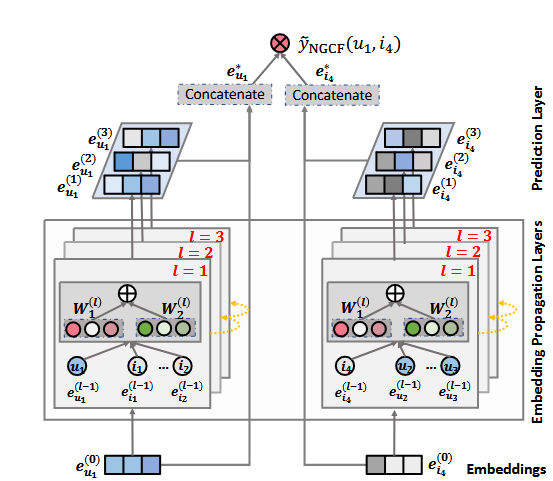
\includegraphics[]{ngcf.png}
	\caption[Αρχιτεκτονική του αλγορίθμου NGCF]{Αρχιτεκτονική του αλγορίθμου NGCF [Πηγή: \url{https://arxiv.org/pdf/1905.08108.pdf}]}
	\label{fig:ngcf}
\end{figure}
Ο NGCF αποτελείται από τρία κύρια στοιχεία:
 \begin{enumerate}
	\item ένα \textit{embedding επίπεδο}, το οποίο περιέχει τα embeddings των χρηστών και των αντικειμένων τα οποία συνενώνονται σε ένα πίνακα αναζήτησης embedding: \begin{align} Ε =[\underbrace{e_{u_1},...,e_{u_N}}_{\substack {\text{embeddings}\\ \text{χρηστών}}}\:, \: \underbrace{e_{i_1},...,e_{i_M}}_{\substack{\text{embeddings} \\ \text{αντικειμένων}}}]
	 \end{align}
	 Στη συνέχεια, ο πίνακας με τα embeddings διαδίδεται μέσω του γράφου χρήστη-αντικειμένου (μια μορφή του οποίου είδαμε στην Εικόνα \ref{fig:graph}), δηλαδή μέσω των επιπέδων διάδοσης embedding
	\item \textit{πολλαπλά επίπεδα διάδοσης embedding (embedding propagation layers)} τα οποία βελτιώνουν τα embeddings ενθέτοντας σε αυτά σχέσεις συνεκτικότητας υψηλής τάξης. Μπορούν να διαδοθούν μέσω αυτών τόσο αλληλεπιδράσεις χαρακτηριστικών υψηλής τάξης, όσο και χαμηλής. Στη διάδοση χαμηλής τάξης  υπάρχουν δύο κύριες διαδικασίες: η \textit{δημιουργία των μηνυμάτων} και η \textit{άθροιση των μηνυμάτων}. Στη δημιουργία των μηνυμάτων για κάθε διασυνδεμένο ζεύγος χρήστη-αντικειμένου $ \left(u, i \right)  $ το μήνυμα από το i στο u ορίζεται ως \begin{align} m_{u \leftarrow i} = \frac{1}{\sqrt{\| N_u\|\|N_i\|}} \bigg(W_1e_i + W_2\left( e_i \odot e_u\right)  \bigg) 
	\end{align} Όπου $ N_u $ και $ N_i $ οι γείτονες του χρήστη u και του αντικειμένου i, κατά την πρώτη μεταβίβαση μηνυμάτων και $ W_1 $, $ W_2 $ τα μητρώα που περιέχουν τα βάρη. Η διαδικασία της άθροισης των μηνυμάτων που έχουν δημιουργηθεί και προέρχονται από την γειτονιά ενός χρήστη u για τον επαναπροσδιορισμό της αναπαράστασης του u γίνεται σύμφωνα με την εξίσωση: 	\begin{align}
	e_u^{(1)} = \text{LeakyReLU}\bigg(m_{u \leftarrow u} + \sum_{i \in N_{u}} m_{u \leftarrow i} \bigg)	
\end{align}
όπου LeakyReLU \cite{maasRectifierNonlinearitiesImprove} είναι η συνάρτηση ενεργοποίησης Ανορθωμένη Γραμμική Μονάδα (Rectified Linear Unit) \begin{equation} 
	LeakyRelU(x) = \begin{cases} 0.01x, & \text{αν}\ x < 0 \\ x, & \text{αλλιώς} \\ \end{cases} 
\end{equation}
 Η διάδοση περιγράφεται σε μορφή μητρώου από τον τύπο:
	\begin{align}
		E^{(l)} = \text{LeakyReLU}\bigg(\left(\mathcal{L}+I\right)E^{(l-1)}W_{1}^{(l)} + \mathcal{L}E^{(l-1)} \odot E^{(l-1)}W_{2}^{(l)} \bigg)
	\end{align}
όπου Ι είναι το ταυτοτικό μητρώο \footnote{Ταυτοτικό μητρώο: ονομάζεται το μητρώο που περιέχει άσσους στην κύρια διαγώνιο και μηδενικά στις υπόλοιπες θέσεις}, W το μητρώο βαρών που χρησιμοποιείται κατά την εκπαίδευση για να εξαχθούν χρήσιμες πληροφορίες για την διάδοση, $ E^{(l)} $ είναι ο πίνακας των embeddings μετά από l βήματα της διάδοσης και $ E^{(0)} $ ο αρχικός πίνακας με τα embeddings, D είναι το διαγώνιο μητρώο, Α το μητρώο γειτνίασης (adjacency matrix) και $ \mathcal{L} $ είναι το Λαπλασιανό μητρώο για τον γράφο χρηστών - αντικειμένων, που περιγράφεται από τη σχέση:
	\begin{align*}
		\mathcal{L} = D^{-\frac{1}{2}}AD^{-\frac{1}{2}} \:, \: A=\begin{bmatrix}
			0 & R \\
			R^{T} & 0\\
		\end{bmatrix}
	\end{align*}
όπου $ R \in \mathbb{R}^{Ν \times Μ} $ το μητρώο αλληλεπίδρασης χρηστών-αντικειμένων
	\item ένα\textit{ επίπεδο πρόβλεψης (prediction layer)} το οποίο αθροίζει τα νέα embeddings, για κάθε χρήστη, τα οποία προέρχονται από διαφορετικά επίπεδα διάδοσης, ώστε να προκύψει το τελικό embedding $e^{\ast}_{u} = e^{(0)}_{u} \| \cdots \|e^{(L)}_{u}$ ,\, $e^{\ast}_{i} = e^{(0)}_{i} \| \cdots \|e^{(L)}_{i}$, με $\|$ συμβολίζεται η πράξη της άθροισης. Τέλος, εξάγει τη βαθμολογία συνάφειας ενός ζεύγους χρήστη-αντικειμένου, δηλαδή την προτίμηση ενός χρήστη u για ένα αντικείμενο i, υπολογίζοντας το εσωτερικό γινόμενο του τελικού embedding με το αντικείμενο.
	\begin{align}
		\hat{y}_{\text{NGCF}}(u, i) = e^{\ast \top}_{u} e^{\ast}_{i}
	\end{align}

\end{enumerate}
Η εκμάθηση των παραμέτρων του μοντέλου, γίνεται μέσω της βελτιστοποίησης της συνάρτησης απώλειας BPR κατά ζεύγη (pairwise BPR loss), που περιγράφεται από την objective συνάρτηση:
\begin{align}
	Loss = \sum_{(u,i,j)\in O}-\ln \sigma(\hat{y}_{ui} - \hat{y}_{uj}) + \lambda \| \Theta \|^{2}_{2}
	\label{eq:ngcf_loss}
\end{align}
με $ \Theta $ συμβολίζονται όλες οι trainable παράμετροι \footnote{ Με τον όρο Trainable  παράμετροι αναφερόμαστε στον αριθμό των βαρών που δεν ενημερώνονται κατά την εκπαίδευση του μοντέλου στον αλγόριθμο οπισθοδιάδοσης (backpropagation).} του μοντέλου, $ \Theta = \left\lbrace E, \left\lbrace W_1^{\left( l \right)} , W_2^{\left( l\right)}  \right\rbrace_{l=1} ^{L} \right\rbrace  $ και $\sigma$ είναι η σιγμοειδής συνάρτηση \begin{equation}
	\label{eq:sigmoid_function}
	\sigma(x) = \frac{1}{1 + e^{-x}}
\end{equation} Οι υπόλοιπες υπερπαράμετροι για τις οποίες υπάρχει και η δυνατότητα ρύθμισης στο Elliot, περιγράφονται στο κάτωθι πλαίσιο.
\begin{tcolorbox}[
colframe=blue!25,
colback=blue!10,
coltitle=blue!20!black,  
fonttitle=\bfseries,
adjusted title= Υπερπαράμετροι]
\textbf{λ}: στο Elliot αναφέρεται ως l\_w και ελέγχει την κανονικοποίηση που εφαρμόζει η L2 στην εξίσωση \eqref{eq:ngcf_loss}, ώστε να αποφευχθεί η υπερεκπαίδευση του μοντέλου.\\
\textbf{message\_dropout:} υποδεικνύει το ποσοστό των εξερχόμενων μηνυμάτων που θα απορριφθούν με τυχαίο τρόπο.\\
\textbf{node\_dropout:} υποδεικνύει το ποσοστό της απόρριψης κόμβων, για την παρεμπόδιση ενός συγκεκριμένου κόμβου, ο οποίος έχει επιλεγεί με τυχαίο τρόπο και ταυτόχρονα απορρίπτει όλα τα εξερχόμενα μηνύματα.\\
\textbf{weight\_size:} αριθμός μονάδων για κάθε επίπεδο διάδοσης embedding.\\
\textbf{n\_fold:} αριθμός πτυχών (folds) για την διάσπαση του μητρώου γειτνίασης σε υπο-μητρώα, με σκοπό τον ευκολότερο υπολογισμό του. 
\end{tcolorbox}
\newpage
\subsubsection{Αλγόριθμος που έχει ως βάση τα τεχνητά νευρωνικά δίκτυα}
\noindent\textbf{DeepFM}\\
O DeepFM \cite{guoDeepFMFactorizationmachineBased2017}  συνδυάζει τα βαθιά νευρωνικά δίκτυα (Deep Neural Networks - DNN) με την τεχνική των Factorization machines. Πιο συγκεκριμένα, αποτελείται από δύο βασικά στοιχεία:
\begin{figure}[H]
	%\vspace{2px}%
	\centering
	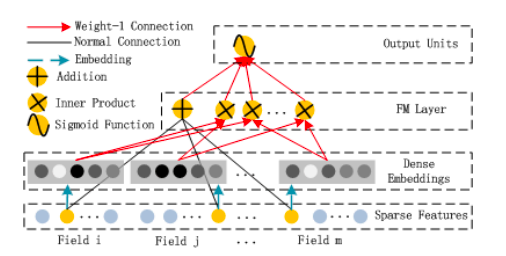
\includegraphics[width=\linewidth]{deepfm.png}
	\caption[Αρχιτεκτονική του αλγορίθμου DeepFM]{Αρχιτεκτονική του αλγορίθμου DeepFM [Πηγή: \url{https://arxiv.org/pdf/1703.04247.pdf}]}
	\label{fig:deepfm}
\end{figure}
\begin{enumerate}
	\item \textbf{Στοιχείο FM του DeepFM:} πρόκειται για την τεχνική των Factorization Machines (FM), η οποία παρουσιάστηκε για πρώτη φορά στο \cite{rendleFactorizationMachines2010} και συνδυάζει την τεχνική της παραγοντοποίησης μητρώου με την παλινδρόμηση. Στην ενότητα 2 περιγράψαμε τους λανθάνοντες παράγοντες και την χρήση τους στα συστήματα συστάσεων. Σε αυτή την τεχνική, οι αλληλεπιδράσεις μεταξύ χρηστών-αντικειμένων αναπαριστώνται με πλειάδες (tuples) διανυσμάτων (λανθανόντων) χαρακτηριστικών (feature vectors) των οποίων οι τιμές είναι πραγματικοί αριθμοί. Έστω $ \mathbf{V} \in \mathbb{R}^{d\times k}  $ τα feature embeddings, τότε $ \mathbf{v}_{i} $ είναι η γραμμή i του V, ενώ με $  \langle \mathbf{v}_i, \mathbf{v}_j \rangle $ αναπαριστάται το εσωτερικό γινόμενο ανάμεσα στις μεταβλητές i και j, το οποίο μοντελοποιεί την αλληλεπίδραση κατά ζεύγη (pairwise) μεταξύ αυτών των δύο μεταβλητών. Επίσης, $ w_{0} $ είναι το global bias, $ w_{i} $ η δύναμη (strength) της μεταβλητής i ενώ με k αναπαριστούμε τον αριθμό των διαστάσεων των λανθανόντων παραγόντων.
	 \begin{align}		
	 \hat{y}_{FM} = \underbrace{\mathbf{w}_0 + \sum_{i=1}^d \mathbf{w}_i x_i }_{\text{παλινδρόμηση}} \:+\underbrace {\sum_{i=1}^d\sum_{j=i+1}^d \langle\mathbf{v}_i, \mathbf{v}_j\rangle x_i x_j}_{\text{παραγοντοποίηση μητρώου}}
    \end{align}
    To στοιχείο αυτό είναι υπεύθυνο για την κάλυψη γραμμικών (1ης τάξης) και pairwise (2ης τάξης) αλληλεπιδράσεων.
	\item\textbf{Στοιχείο Deep (learning) του DeepFM:} είναι ένα feed-forward νευρωνικό δίκτυο \cite{hoffmannSimulationNeuronalerNetze1992} και πιο συγκεκριμένα ένα πολυεπίπεδο Perceptron (Multilayer Perceptron - MLP), το οποίο χρησιμοποιείται για την εκμάθηση αλληλεπιδράσεων χαρακτηριστικών υψηλής τάξης. Στα feedforward νευρωνικά δίκτυα η πληροφορία διαχέεται μόνο προς μια κατεύθυνση: προς το επόμενο επίπεδο, δηλαδή προς τα εμπρός (forward), χωρίς να δημιουργούνται κύκλοι. Αναλυτικότερα από τα επίπεδα εισόδου μεταβαίνει απευθείας στα κρυφά επίπεδα και από εκεί στα επίπεδα εξόδου. Το στοιχείο Deep του DeepFM, όπως και όλα τα MLPs, αποτελείται από τα εξής επίπεδα:\begin{itemize}
		\item \textbf{Επίπεδο εισόδου (input layer):} αποτελείται από δύο υποεπίπεδα, το πρώτο λαμβάνει ως είσοδο τα ανεπεξέργαστα αραιά χαρακτηριστικά και το δεύτερο embedding επίπεδο μετατρέπει αυτά τα χαρακτηριστικά σε πυκνά embeddings, χαμηλών διαστάσεων.
		\item \textbf{Κρυφό επίπεδο (hidden layer):} λαμβάνει ως είσοδο τα embeddings που παρήχθησαν από το embedding επίπεδο, του επιπέδου εισόδου και παράγει ως έξοδο ένα πυκνό διάνυσμα χαρακτηριστικών, του οποίου οι τιμές ανήκουν στο σύνολο των πραγματικών αριθμών.
		\item \textbf{Επίπεδο εξόδου (output layer):} λαμβάνει ως είσοδο το διάνυσμα που παρήγαγε το προηγούμενο επίπεδο και «τροφοδοτεί» με αυτό τη σιγμοειδή συνάρτηση:
		 \begin{align}		
			\hat{y}_{DNN} = sigmoid\left({W^{|H|+1}}\ast{a^{|H|}} + b^{|H|+1}\right)
		\end{align}
	όπου Η ο αριθμός των κρυφών επιπέδων.
	\end{itemize} 
    Η πρόβλεψη που δίνεται από το τελευταίο επίπεδο του νευρωνικού δικτύου του αλγορίθμου υπολογίζεται από τον τύπο:
	 \begin{align}		
	  \hat{y} = sigmoid\left( y_{FM} + y_{DNN}\right) 
    \end{align}
δηλαδή από την σιγμοειδή συνάρτηση του αθροίσματος των δύο κύριων στοιχείων του αλγορίθμου, του FM και του Deep.
\end{enumerate}
Στην Εικόνα \ref{fig:deepfm} παρουσιάζεται η αρχιτεκτονική του αλγορίθμου, όπως αυτή παρουσιάστηκε στο \cite{guoDeepFMFactorizationMachineBased2017} .
\begin{tcolorbox}[
	colframe=blue!25,
	colback=blue!10,
	coltitle=blue!20!black,  
	fonttitle=\bfseries,
	adjusted title= Υπερπαράμετροι]
	\textbf{hidden\_neurons:} ο αριθμός των νευρώνων σε κάθε επίπεδο, η αύξησή τους προκαλεί και αύξηση της πολυπλοκότητας.\\
	\textbf{hidden\_activations:} λίστα η οποία περιέχει τις συναρτήσεις ενεργοποίησης (activation functions), οι οποίες καθορίζουν την έξοδο ενός κόμβου σε ένα νευρωνικό δίκτυο.\\
	\textbf{l\_w:} παράμετρος κανονικοποίησης στα Embeddings χρηστών και αντικειμένων.

\end{tcolorbox}
\subsubsection{Μη-εξατομικευμένοι αλγόριθμοι}
\noindent Στα συστήματα συστάσεων αυτού του είδους όλοι οι χρήστες λαμβάνουν τις ίδιες ακριβώς λίστες συστάσεων, εν αντιθέσει με τα εξατομικευμένα συστήματα συστάσεων (personalized recommender systems) τα οποία προτείνουν σε κάθε χρήστη αντικείμενα με βάση προηγούμενες αλληλεπιδράσεις του. Χαρακτηριστικότερο παράδειγμα μη-εξατομικευμένου συστήματος συστάσεων αποτελεί ο αλγόριθμος \textbf{Most popular (MostPop}) ο οποίος προτείνει σε κάθε χρήστη τα πιο δημοφιλή αντικείμενα. Σε αυτήν την κατηγορία ανήκει επίσης και ο αλγόριθμος \textbf{Random} ο οποίος επιλέγει αντικείμενα με τυχαίο τρόπο από το σύνολο των διαθέσιμων αντικειμένων, ακολουθώντας την κανονική κατανομή, αποφεύγοντας τα αντικείμενα που έχουν ήδη καταναλωθεί και τα προτείνει στους χρήστες. Όπως γίνεται εύκολα αντιληπτό, αυτός ο αλγόριθμος δεν πετυχαίνει καλή ακρίβεια ειδικά αν είναι μεγάλος ο αριθμός των αντικειμένων, και η απόδοσή του εξαρτάται από την τύχη, επομένως χρησιμοποιείται μόνο για πειραματικούς σκοπούς όπως θα δείξουμε και στη συνέχεια.  Οι αλγόριθμοι αυτοί χρησιμοποιούνται ως baseline (MostPop χειρότερη επίδοση και Random την καλύτερη σε ότι αφορά το popularity bias) και συγκρίνονται με τους αλγορίθμους που αναλύσαμε παραπάνω, προκειμένου να εξάγουμε πιο ασφαλή συμπεράσματα κυρίως σε ό,τι αφορά το popularity bias.
\subsection{Μετρικές αξιολόγησης}
\noindent Για την αξιολόγηση των αποτελεσμάτων, δηλαδή των λιστών συστάσεων που παρήγαγαν οι αλγόριθμοι που περιγράψαμε, χρησιμοποιήθηκαν τέσσερις μετρικές ακρίβειας, πέντε μετρικές popularity bias, μία μετρική κάλυψης αντικειμένων, μία μετρική diversity και μια μετρική novelty. Ακολουθεί η αναλυτική περιγραφή τους.
\subsubsection{Μετρικές ακρίβειας}
\noindent\textbf{Normalized discounted cumulative gain (nDCG):} \cite{jarvelinCumulatedGainbasedEvaluation2002},  \cite{jarvelinIREvaluationMethods2000} ο βαθμός στον οποίο η κατάταξη που υπέβαλε ένας χρήστης συμφωνεί με την ιδανική κατάταξη, λαμβάνοντας υπόψη τη συνάφεια κάθε στοιχείου σε αυτήν τη λίστα αντικειμένων για κατάταξη. Ακολουθούν τα αναλυτικά βήματα υπολογισμού του nDCG.
Κάθε πρόταση (recommendation) έχει μια βαθμολογία σχετικότητας (relevance score), η οποία ονομάζεται και κέρδος (gain). Το  αθροιστικό κέρδος (cumulative gain) μας δίνει το άθροισμα όλων των βαθμολογιών σχετικότητας.
\begin{align}
	\text{CumulativeGain}\left(CG\right)= \sum_{i=1}^{n}{relevance}_i
\end{align}
Ωστόσο, το cumulative gain δεν λαμβάνει καθόλου υπόψη του την θέση των στοιχείων στη λίστα κατάταξης, κάτι αρκετά σημαντικό σε μια εργασία κατάταξης αντικειμένων (ranking task). Το Discounted Cumulative Gain (DCG) προσθέτει έναν λογαριθμικό παράγοντα αναγωγής (reduction factor) προκειμένου να «τιμωρήσει» (penalize) την βαθμολογία σχετικότητας αναλογικά με τη θέση του αντικειμένου
\begin{align}
	\text{DiscountedCumulativeGain}\left(DCG\right)= \sum_{i=1}^{n}\frac{{relevance}_i}{\log_2{\left(i+1\right)}}
\end{align}
Ένα πρόβλημα που προκύπτει με το DCG είναι πως στους χρήστες θα προταθεί ένας αρκετά μεταβλητός αριθμός σχετικών αντικειμένων. Οπότε θα είναι αρκετά δύσκολο να γίνουν συγκρίσεις ανάμεσα στους χρήστες. Για αυτόν τον λόγο κρίνεται απαραίτητη μια κανονικοποίηση των αποτελεσμάτων που παράγει η μετρική ώστε να βρίσκονται στο εύρος [0,1], η οποία θα μας δώσει την ιδανική κατάταξη για έναν χρήστη. Στη συνέχεια, χρησιμοποιούμε αυτή την κατάταξη ως το Ideal Discounted Cumulative Gain (IDCG)
\begin{align}
	\text{IdealDiscountedCumulativeGain}\left(IDCG\right)= \sum_{i=1}^{REL_n}\frac{2^{{rel}_i}-1}{\log_2{\left(i+1\right)}} 
\end{align}
όπου $ {rel}_i $ η σχετικότητα του αντικειμένου στη θέση i στη λίστα συστάσεων και $ 2^{{rel}_i}=1 $ αν είναι σχετικό (hit) αλλιώς είναι ίσο με 0.
To nDCG είναι ο λόγος του DCG προς το IDCG
\begin{align}
	\text{Normalized Discounted Cumulative Gain}\left(nDCG\right)=\frac{DCG}{IDCG}
\end{align}
\\
\noindent \textbf{Precision} ή true positive accuracy ή εμπιστοσύνη (confidence) είναι το ποσοστό των συστάσεων που ορθά προτάθηκαν από τον αλγόριθμο (True Positive) σε σχέση με το σύνολο των συστάσεων - ορθών και λανθασμένων (True positive + False positive):\\
\begin{align}
	 precision=\ tpa=\ \frac{tp}{tp+fp}
 \end{align}\\
\textbf{Ανάκληση (Recall):} ή true positive rate ή ευαισθησία (sensitivity). Υπολογίζει το ποσοστό των αντικειμένων που έχουν προταθεί και είναι σχετικά σε σχέση με τον συνολικό αριθμό των σχετικών αντικειμένων. Με άλλα λόγια, το ποσοστό των συστάσεων που ορθά προτάθηκαν από τον αλγόριθμο (True Positive) σε σχέση με το (ιδανικό) σύνολο όλων των συστάσεων που θα μπορούσαν να προταθούν:\\
\begin{align}
 recall=\ tpr=\ \frac{tp}{tp+fn} 
\end{align} 
\textbf{Hit Rate (HR)} \cite{deshpandeItemBasedTopNRecommendation2004}\\
Ο αριθμός των hits είναι ο αριθμός των αντικειμένων στο σύνολο δοκιμής το οποία εμφανίζονται επίσης και στα Top-n αντικείμενα που δίνονται ως συστάσεις σε κάθε χρήστη.
\begin{align}
\mathrm {HR@K} =\frac{\text{Αριθμός} \: \text{των} \: \text{Hits} @K}{\text{Αριθμός χρηστών}}
\end{align} 
Εάν το hit rate είναι ίσο με 1 αυτό σημαίνει πως ο αλγόριθμος έχει εντοπίσει όλα τα «κρυφά» αντικείμενα.
\subsubsection{Μετρικές μεροληψίας δημοφιλίας}
\noindent \textbf{Μέση δημοφιλία των συστάσεων - Average Recommendation Popularity (ARP):}  Αυτή η μετρική \cite{yinChallengingLongTail2012a} υπολογίζει τη μέση δημοφιλία (average popularity) των αντικειμένων που προτείνονται σε κάθε λίστα. 
\begin{align}
	{ARP}=\frac{1}{\left|U_{t}\right|} \sum_{u \in U_{t}} \frac{\sum_{i \in L_{u}} \varphi(i)}{\left|L_{u}\right|} 
\end{align}
\\όπου $ \bm{{\varphi\left(i\right)}}$ είναι ο αριθμός των φορών που το αντικείμενο (item) i έχει αξιολογηθεί στο σύνολο εκπαίδευσης,  $ L_{u}  $ είναι η λίστα των προτεινόμενων αντικειμένων για τον χρήστη u και $ U_{t} $ είναι ο αριθμός των χρηστών στο σύνολο δοκιμής.\\\\
\textbf{Μέσο ποσοστό των long tail αντικειμένων - Average Percentage of Long Tail Items\\ (APLT):}  αυτή η μετρική που ορίζεται στο \cite{abdollahpouriControllingPopularityBias2017}, μετράει το μέσο ποσοστό των long tail αντικειμένων στις λίστες συστάσεων, δηλαδή το μέσο ποσοστό των αντικειμένων στις λίστες συστάσεων, που δημιουργούνται για κάθε χρήστη, που ανήκουν στο σύνολο των long tail αντικειμένων $ {\Gamma} $ 
\begin{align}
	APLT=\ \frac{1}{U_t}\sum_{u\in U_t}\frac{\left|\left\{i,i\in\left(L_u\cap{\Gamma}\right)\right\}\right|}{\left|L_u\right|}
\end{align}\\
\textbf{Μέση κάλυψη των long-tail αντικειμένων - Average Coverage of Long Tail items (ACLT):}  Ένα πρόβλημα με την μετρική APLT είναι πως μπορεί να έχει υψηλή τιμή ακόμη και αν όλοι οι χρήστες λάβουν το ίδιο σύνολο long tail αντικειμένων. Μια λύση σε αυτό το πρόβλημα δόθηκε στο \cite{abdollahpouriManagingPopularityBias2019a}, μέσω της μετρικής ACLT, μια ακόμη μετρική για την αξιολόγηση της έκθεσης των long tail αντικειμένων στις λίστες συστάσεων.
\begin{align}
	ACLT=\ \frac{1}{U_t}\sum_{u\in U_t}\sum_{i\in L_u}1\left(i\in{\Gamma}\right)
\end{align}
\\

\noindent Τέλος, χρησιμοποιήθηκαν 2 μετρικές που ορίζονται στο \cite{zhuMeasuringMitigatingItem2020}\\
\textbf{Popularity Ranking-based Statistical Parity (PopRSP):} υπολογίζει κατά πόσο η πιθανότητα να προταθούν αντικείμενα που ανήκουν στο long-tail και η πιθανότητα να προταθούν αντικείμενα που ανήκουν στο head είναι ίδια
\begin{align}
	{RSP}=\frac{{std}\left(P\left(R @ k \mid g=g_{1}\right), \ldots, P\left(R @ k \mid g=g_{A}\right)\right)}
	{{mean}\left(P\left(R @ k \mid g=g_{1}\right), \ldots, P\left(R @ k \mid g=g_{A}\right)\right)}
\end{align}
\textbf{Popularity Ranking-based Equal Opportunity (PopREO):} υπολογίζει κατά πόσο τα true positive rates των αντικειμένων που ανήκουν στο long-tail και των αντικειμένων που ανήκουν στο head είναι ίδια, λαμβάνοντας υπόψη τις προτιμήσεις των χρηστών. 
\begin{align}
	{REO}=\frac{{std}\left(P\left(R @ k \mid g=g_{1}, y=1\right) \ldots P\left(R(a) k=g_{A}, y=1\right)\right)}
	{{mean}\left(P\left(R @ k \mid g=g_{1}, y=1\right) \ldots P\left(R @ k \mid g=g_{A}, y=1\right)\right)}
\end{align}
\subsubsection{Μετρικές diversity}
\noindent \textbf{Gini index \cite{giniMeasurementInequalityIncomes1921}:} υπολογίζει την ανισότητα που υπάρχει στην κατανομή συχνότητας των προτεινόμενων αντικειμένων και συνεπώς το diversity που υπάρχει στα αποτελέσματα. Η τιμή του gini index είναι υψηλή εάν ορισμένα αντικείμενα προτείνονται πιο συχνά σε σχέση με άλλα αντικείμενα. Επομένως ένας αλγόριθμος που ακολουθεί την κανονική κατανομή σε ότι αφορά τις συστάσεις των αντικειμένων και προτείνει κάθε αντικείμενο ίδιο αριθμό φορών, θα έχει gini index ίσο με $ 0 $. Στην αντίθετη περίπτωση, όπου ο αριθμός των φορών που προτείνονται τα διαφορετικά αντικείμενα είναι αρκετά άνισος, τότε η μετρική αυτή θα είναι ίση με 1. Το gini index ορίζεται ως εξής:
\begin{align}
	{GiniIndex}=\frac{1}{n-1} \sum_{j=1}^{n}(2 j-n-1) p\left(i_{j}\right)
\end{align}
Σε αυτό το σημείο κρίνεται αναγκαίο να επισημάνουμε πως στο Elliot η μετρική αυτή διαφοροποιείται και υπολογίζεται το $ 1 - Gini $, ώστε υψηλή τιμή του Gini index να σημαίνει καλύτερο αποτέλεσμα διευκολύνοντας έτσι τον αναγνώστη. 
\subsubsection{Μετρικές novelty}
\noindent\textbf{Expected Popularity Complement (EPC):} \cite{vargasRankRelevanceNovelty2011} αξιολογεί τον αναμενόμενο αριθμό σχετικών αντικειμένων που δεν είχε δει προηγουμένως ο χρήστης. Ένα
σύστημα συστάσεων λαμβάνει υψηλότερη τιμή EPC όταν όχι μόνο προτείνει αντικείμενα από το long tail,
αλλά τα κατατάσσει επίσης ψηλά στις λίστες συστάσεων. Εάν το σύστημα συστάσεων προτείνει αντικείμενα
με χαμηλή εκτιμώμενη έκθεση, τότε το EPC θα είναι κοντά στο ένα. 
\begin{align}
	{EPC}=C \sum_{i_{k} \in R} \operatorname{disc}(k) p\left(r e l \mid i_{k}, u\right)\left(1-p\left(\operatorname{seen} \mid i_{k}\right)\right)
\end{align}
Όπου \begin{itemize}
	\item $ p\left(seen\mid i_k\right) $ είναι η πιθανότητα ένας χρήστης να δει το αντικείμενο i 
	\item $ p\left(rel\mid i_k,u\right) $ δηλώνει την πιθανότητα το αντικείμενο i που βρίσκεται στη θέση k της κατάταξης των αντικειμένων στη λίστα συστάσεων, να είναι σχετικό για τον χρήστη u.
	\item C είναι μια σταθερά κανονικοποίησης, της οποίας ο σκοπός είναι να σταθεροποιήσει την μετρική και να μην εισαχθεί κάποια ανεπιθύμητη μεροληψία σε αυτή.
	\begin{align*}
	C = \frac{1}{\sum_{i_{k} \in R} \operatorname{disc}(k)}
    \end{align*} 
\item $ disc\left(k\right) $ έστω ότι ένας χρήστης περιηγείται τα αντικείμενα μιας λίστας με τη σειρά κατάταξής τους, έως ότου σταματήσει. Σε κάθε θέση k της κατάταξης, ο χρήστης λαμβάνει την απόφαση για το αν θα συνεχίσει ή όχι. Στόχος είναι να βρούμε την πιθανότητα ένας χρήστης u να συνεχίσει μειώνοντας όσο γίνεται περισσότερο την υπολογιστική πολυπλοκότητα είναι. Προκειμένου να συμβεί αυτό χρησιμοποιούμε μια συνάρτηση έκπτωσης (discount function) η οποία εκφράζει το γεγονός ότι όσο πιο χαμηλά είναι ένα αντικείμενο στη λίστα τόσο λιγότερες είναι οι πιθανότητες να το δει ένας χρήστης.
\end{itemize}
\subsubsection{Μετρικές coverage}
\noindent\textbf{Item Coverage:} \cite{adomaviciusImprovingAggregateRecommendation2012} υπολογίζει τον συνολικό αριθμό των (μοναδικών) αντικειμένων που έχουν προταθεί από έναν αλγόριθμο σε όλους τους χρήστες ενός συνόλου δεδομένων.
\begin{align}
	\text{Item coverage} = |\cup_{u \in U}L_{n}(u)|
\end{align}
όπου $  L_{n}(u) = \left\lbrace i_1 \cdots \i_N \right\rbrace $ η λίστα των $ N $ αντικειμένων που έχουν προταθεί στον χρήστη $ u $.
%%%%%%%%%%%%%%%%%%%%%%%%%%%%%%%%
% Eπεξεργασια και οπτικοποιηση %
%%%%%%%%%%%%%%%%%%%%%%%%%%%%%%%%
\newpage
\section{Επεξεργασία και οπτικοποίηση συνόλων δεδομένων} \label{data_proc}
\noindent Ύστερα από ανάλυση των συνόλων δεδομένων που αντλήσαμε από το διαδίκτυο, προέκυψε πως δεν χρειάζονται κάποια επεξεργασία και μπορούν να χρησιμοποιηθούν άμεσα.\\
\noindent Το σύνολο δεδομένων στο οποίο χρειάστηκε να γίνει η μεγαλύτερη επεξεργασία είναι το Elec\_retailer. Αυτό ήταν αναμενόμενο καθώς είναι το μοναδικό από τα τέσσερα σύνολα δεδομένων που είναι «πραγματικό», δηλαδή προέρχεται κατευθείαν από την βάση δεδομένων μιας εταιρείας έχοντας υποστεί ελάχιστη ή και καθόλου επεξεργασία. Αρχικά, για πάνω από 200 αξιολογήσεις που υπήρχαν στο Elec\_retailer υπήρχε μόνο ο υπερσύνδεσμος για το προϊόν και όχι το ID και χρειάστηκε να βρούμε το ID του, επισκέπτοντας τον αντίστοιχο σύνδεσμο για κάθε μία αξιολόγηση, κάτι που κόστισε αρκετό χρόνο. Σε αυτό το σημείο θα πρέπει να αναφερθεί πως υπήρχαν περίπου 700 κριτικές προϊόντων χωρίς να υπάρχει διαθέσιμο το ID του προϊόντος, η ονομασία του ή έστω κάποιος σύνδεσμος που να οδηγεί σε αυτό. Επειδή η διαδικασία εύρεσης αυτών των προϊόντων ήταν από δύσκολη έως αδύνατη σε πολλές περιπτώσεις, αλλά και αρκετά χρονοβόρα λάβαμε την απόφαση αυτές οι κριτικές να απορριφθούν. Από την παραπάνω επεξεργασία του συνόλου δεδομένων απέμειναν 3.078 προϊόντα και 8.263 αξιολογήσεις. Ένα από τα μεγαλύτερα προβλήματα που υπήρχαν εδώ, ήταν η απουσία κάθε πληροφορίας για τους χρήστες, ένα από τα τρία πιο σημαντικά στοιχεία για τα συστήματα συστάσεων που ερευνούμε (τα υπόλοιπα δύο είναι φυσικά πληροφορίες για τις αξιολογήσεις και για τα αντικείμενα). Το πρόβλημα μετατράπηκε σε μία μεγάλη και ωραία πρόκληση, καθώς μας οδήγησε σε διαφορετικά ερευνητικά μονοπάτια. Αυτό συνέβη διότι, η δημιουργία των χρηστών δεν ήταν απλή υπόθεση, δηλαδή δεν θα ήταν επιστημονικά ορθό να επιλέξουμε έναν τυχαίο αριθμό χρηστών και να τους δημιουργήσουμε. Έπρεπε να λάβουμε υπόψη μας διάφορες παραμέτρους και κυρίως το πρόβλημα της αραιότητας του μητρώου χρηστών-αντικειμένων, το οποίο εξαρτάται άμεσα και από τον αριθμό των χρηστών που υπάρχουν σε ένα σύνολο δεδομένων. Με γνώμονα όλα τα παραπάνω δημιουργήθηκαν 3 διαφορετικά σύνολα δεδομένων, με 3 διαφορετικούς αριθμούς χρηστών:
\begin{enumerate}
	\item \textbf{Elec\_retailer30:} 276 χρήστες, εκ των οποίων οι 275 έχουν αξιολογήσει 30 προϊόντα ο καθένας και ένας 13 προϊόντα.
		\vspace{-2.50mm}
	\item \textbf{Elec\_retailer20:} 414 χρήστες, εκ των οποίων οι 413 έχουν αξιολογήσει 20 προϊόντα ο καθένας και ένας 3 προϊόντα.
		\vspace{-2.50mm}
	\item \textbf{Elec\_retailer10:}	826 χρήστες, εκ των οποίων οι 825 έχουν αξιολογήσει 10 προϊόντα ο καθένας και ένας 3 προϊόντα.
\end{enumerate}
\noindent Για όλα τα σύνολα δεδομένων που χρησιμοποιήθηκαν έγινε με τυχαίο τρόπο η διάσπασή τους σε 2 μικρότερα σύνολα δεδομένων. Πιο συγκεκριμένα, το 80\% αποτέλεσε το σύνολο εκπαίδευσης και το 20\% το σύνολο δοκιμής.\\
Ύστερα από την ολοκλήρωση της επεξεργασίας των δεδομένων, σειρά έχει η οπτικοποίησή τους για την καλύτερη κατανόησή τους, η οποία θα βοηθήσει αρκετά στη συνέχεια, τόσο στη ρύθμιση των υπερπαραμέτρων των αλγορίθμων συστημάτων συστάσεων, όσο και στην αξιολόγησή τους.
 \noindent Αρχικά, για την παρατήρηση του φαινομένου long-tail δημιουργήθηκε το κάτωθι γράφημα, στο οποίο το 20\% των αντικείμενων που έχουν λάβει τις περισσότερες αξιολογήσεις, δηλαδή τα πιο δημοφιλή αντικείμενα, ανήκει στο head, και το υπόλοιπο 80\% αφορά λιγότερο δημοφιλείς ή καινούριες ταινίες. Πιο συγκεκριμένα, στον άξονα x είναι τα IDs των ταινιών διατεταγμένα κατά φθίνουσα σειρά ως προς τον αριθμό των αξιολογήσεων που έχουν λάβει και στον άξονα y ο συνολικός αριθμός των αξιολογήσεων που έλαβε κάθε ταινία. Από το διάγραμμα αυτό είναι αρκετά ευδιάκριτο το φαινόμενο του long tail, καθώς περίπου 700 ταινίες έχουν λάβει από 500 έως και περίπου 3.500 αξιολογήσεις η κάθε μία, ενώ 3.000 ταινίες έχουν λάβει από λίγες έως ελάχιστες αξιολογήσεις.
 \begin{figure}[H]
 	%\vspace{2px}%
 	\centering
 	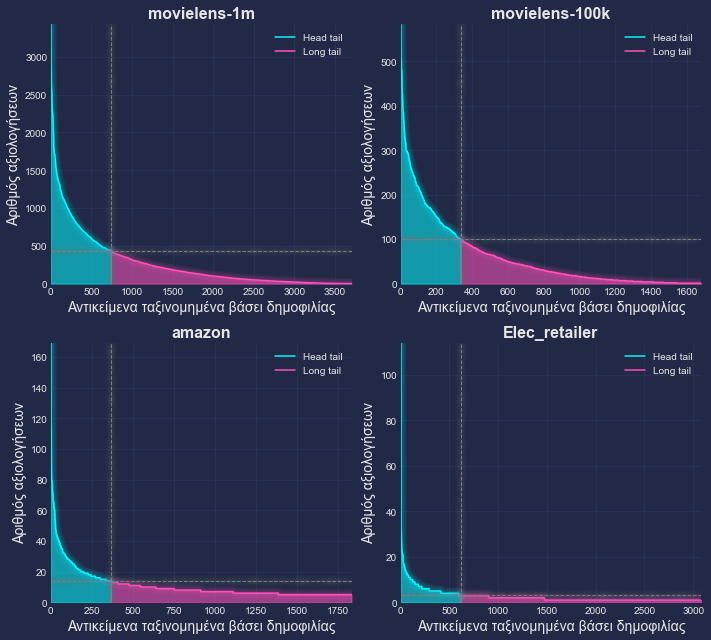
\includegraphics[width=\linewidth]{pop_diagram.png}
 	\caption{Το φαινόμενο του long-tail στα 4 σύνολα δεδομένων}
 	\label{fig:pop}
 	\vspace{-5.50mm}
 \end{figure}
\vspace{0.00mm}
 \noindent Στην Εικόνα \ref{fig:density} παρουσιάζεται για κάθε σύνολο δεδομένων ένα διάγραμμα το οποίο θα μας βοηθήσει να κατανοήσουμε καλύτερα την κατανομή των αξιολογήσεων. Στον άξονα x έχουμε τον μέσο όρο των αξιολογήσεων των αντικειμένων και στον άξονα y την Εκτίμηση πυκνότητας πυρήνα (Kernel Density Estimation - KDE), όπου όλα τα σημεία του χώρου λαμβάνουν κάποια τιμή η οποία δείχνει ότι υπάρχει συγκεκριμένη πιθανότητα επίσκεψής τους. Προκειμένου να γίνει πιο κατανοητή η έννοια του μέσου όρου των αξιολογήσεων ας δούμε ένα παράδειγμα. Έστω ότι μια ταινία έχει αξιολογηθεί τέσσερις φορές και έχει λάβει τις βαθμολογίες 2, 2, 3 και 5. Τότε ο μέσος όρος αξιολόγησης αυτής της ταινίας είναι $ \frac{2+2+3+5}{4} = \frac{15}{4}=3,75 $.
Στα σύνολα δεδομένων από τον χώρο του ηλεκτρονικού εμπορίου η συντριπτική πλειονότητα των αντικειμένων έχει μέσο όρο αξιολογήσεων μεγαλύτερο του 3,5. Αντιθέτως, στα σύνολα δεδομένων του Movielens υπάρχει πολύ μεγαλύτερη ισορροπία και μάλιστα η κατανομή τους είναι αρκετά στην κανονική κατανομή, κάτι που είναι ευδιάκριτο από τα διαγράμματα.
\begin{figure}[htp]
	\vspace{0.00mm}
	\centering
	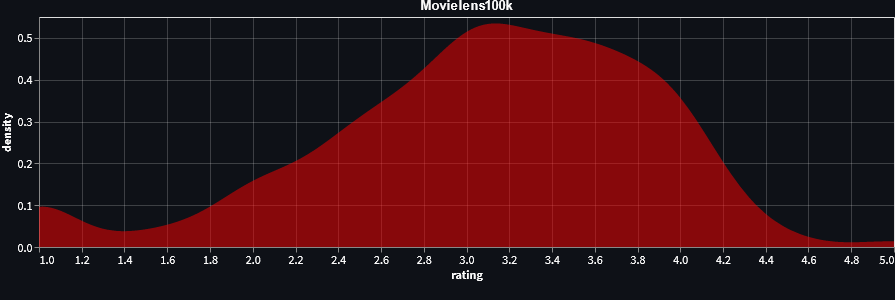
\includegraphics[width=\linewidth]{visualization_ml100k.png}
	\vspace{-0.20mm}
		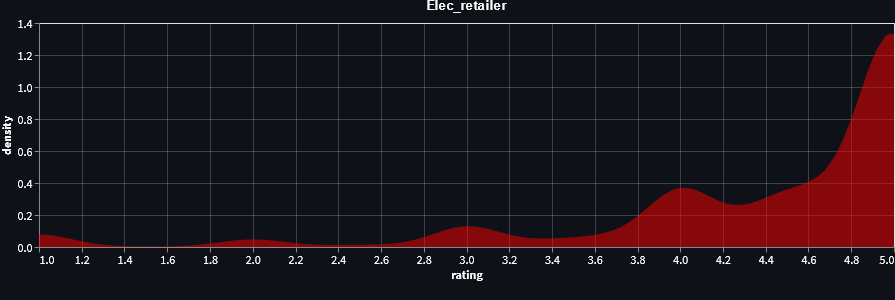
\includegraphics[width=\linewidth]{visualization_1.png}
		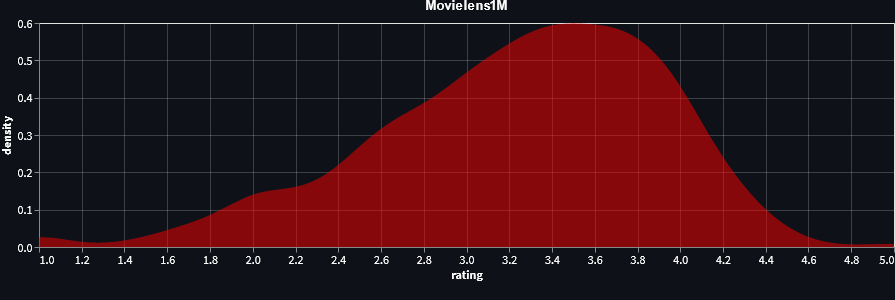
\includegraphics[width=\linewidth]{visualization_3.png}
			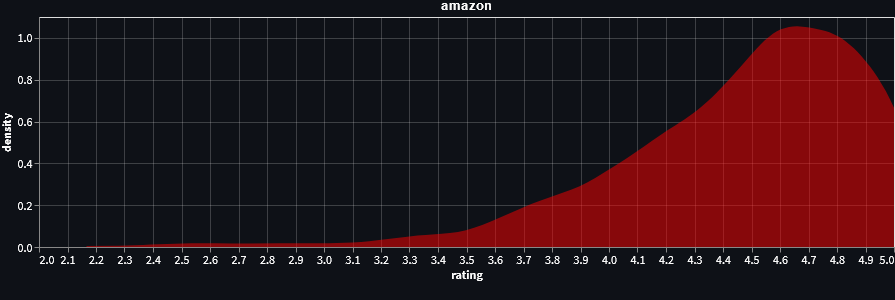
\includegraphics[width=\linewidth]{visualization_amazon.png}
	\caption{Κατανομή μέσης αξιολόγησης ανά αντικείμενο στα 4 σύνολα δεδομένων}
	\label{fig:density}
\end{figure}


\newpage
\section{Αξιολόγηση αποτελεσμάτων}
\noindent Αφού δημιουργήσαμε τις λίστες συστάσεων στο προηγούμενο βήμα στην ενότητα αυτή παρουσιάζουμε και αναλύουμε τα αποτελέσματα της αξιολόγησης αυτών των συστάσεων ως προς την ακρίβεια, τo popularity bias, το diversity, το novelty και την κάλυψη των αντικειμένων, όπως αυτά προέκυψαν από τις μετρικές αξιολόγησης που επιλέξαμε. Στις υποενότητες που ακολουθούν θα βρείτε δύο τύπους ανάλυσης την «Ανάλυση υπερπαραμέτρων» και την «Ανάλυση καλύτερων αποτελεσμάτων». Γενικότερα στην παρούσα ενότητα, θα επιχειρήσουμε να απαντήσουμε τα εξής ερωτήματα:
\begin{enumerate}
	\item Εκτός της ακρίβειας, επηρεάζουν οι διαφορετικές τιμές των υπερπαραμέτρων το popularity bias, το diversity, το novelty και την κάλυψη των αντικειμένων, και αν ναι σε ποιον βαθμό;
	\item Ποια είναι η συμπεριφορά των οικογενειών αλγορίθμων ειδικότερα και των διάφορων αλγορίθμων γενικότερα, απέναντι σύνολα δεδομένων που χρησιμοποιήθηκαν; Είναι αυτό εφικτό να επιτευχθεί σε όλες τις περιπτώσεις;
	\item Ποιες οι βέλτιστες τιμές των υπερπαραμέτρων ώστε να επιτευχθεί το αντιστάθμισμα μεροληψίας-ακρίβειας;
	\item Επηρεάζουν τα χαρακτηριστικά των δεδομένων τα αποτελέσματα;
	\item Ποιες είναι οι επιπτώσεις από τη λάθος επιλογή ενός αλγορίθμου ή/και των υπερπαραμέτρων του;
	
\end{enumerate}
\noindent Προκειμένου να εξάγουμε όσο το δυνατόν πιο ασφαλή συμπεράσματα, στην «Ανάλυση υπερπαραμέτρων» και στον «Μετριασμό της μεροληψίας» δεν χρησιμοποιήθηκε το σύνολο δεδομένων Elec\_retailer στο οποίο έχουμε δημιουργήσει μόνοι μας τους χρήστες, όπως προαναφέρθηκε, και επομένως είναι υπαρκτός ο κίνδυνος να έχουμε εισάγει κάποιο είδος μεροληψίας άθελά μας.
\begin{tcolorbox}[
	colframe=blue!25,
	colback=blue!10,
	coltitle=blue!20!black,  
	fonttitle=\bfseries,
	adjusted title= Σημείωση]
	Όλοι οι πίνακες που δημιουργήθηκαν στην παρούσα ενότητα χρησιμοποιούν την κάτωθι χρωματική διαβάθμιση, προκειμένου να διευκολύνουν τον αναγνώστη να διαχωρίσει τα καλύτερα από τα χειρότερα αποτελέσματα. Εδώ απαιτείται ιδιαίτερη προσοχή, καθώς στις μετρικές PopREO, PopRSP και ARP όσο μεγαλύτερη είναι η τιμή τους, τόσο μεγαλύτερη είναι η μεροληψία που εισάγεται.\\
	
		%\vspace{2px}%
		\centering
		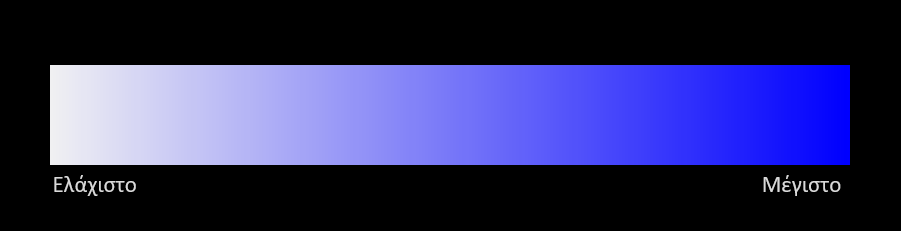
\includegraphics[width=\linewidth]{output1.png}
		%	\caption{Σελίδα δημιουργίας συστήματος συστάσεων}
		\label{fig:scale}
	
\end{tcolorbox}
\newpage
\subsection{Ανάλυση υπερπαραμέτρων}
\noindent Προτού προχωρήσουμε όμως στην ανάλυση των υπερπαραμέτρων κρίνεται αναγκαίο να δοθούν ορισμένες διευκρινίσεις. Αρχικά, στον πίνακα \ref{tab:alg_hyper} παρουσιάζονται όλοι οι αλγόριθμοι που χρησιμοποιήθηκαν στα πειράματα - εκτός από τους δύο μη-εξατομικευμένους - , μαζί με όλες τις τιμές των υπερπαραμέτρων που επιλέχθηκαν. Σε παρένθεση βρίσκεται η συντομογραφία της ονομασίας των υπερπαραμέτρων που χρησιμοποιείται στους πίνακες μέσω των οποίων παρουσιάζονται τα αποτελέσματα, χάριν εξοικονόμησης χώρου.\\ Στο σημείο αυτό θα πρέπει να σημειωθεί ότι εξαιτίας του μεγάλου όγκου των δεδομένων που προέκυψαν από την εκτέλεση κάθε αλγορίθμου για τρία διαφορετικά σύνολα δεδομένων και διάφορες τιμές των υπερπαραμέτρων και την αξιολόγηση από δώδεκα διαφορετικές μετρικές αξιολόγησης, στην ανάλυση που ακολουθεί δεν παρουσιάζονται όλες οι μετρικές, προς διευκόλυνση του αναγνώστη. Από τις μετρικές ακρίβειας έχει επιλεγεί η nDCG και από τις μετρικές μεροληψίας δημοφιλίας οι ARP, APLT, PopREO, PopRSP, μαζί με τις μετρικές EPC, Gini index και Item coverage.\\ Επιπροσθέτως, οι τιμές του μεγέθους των λιστών συστάσεων που θα ληφθούν υπόψη κατά τον υπολογισμό των μετρικών αξιολόγησης (cut-off) είναι: [10, 30, 50, 70, 100], ενώ η τιμή του cut-off που επιλέχθηκε για την ανάλυση των υπερπαραμέτρων είναι η 100, καθώς χρησιμοποιείται αρκετά συχνά στην βιβλιογραφία και είναι κατάλληλη σύμφωνα με τα χαρακτηριστικά των δεδομένων των συνόλων δεδομένων που χρησιμοποιήθηκαν. Τέλος, η μετρική ομοιότητας ``dot" στους αλγορίθμους ItemKNN και UserKNN, είχε πολύ κακή επίδοση για όλα τα σύνολα δεδομένων και όλες τις μετρικές αξιολόγησης και για τον λόγο αυτό δεν παρουσιάζεται στην ανάλυση που ακολουθεί, ώστε να μην μπερδέψει τον αναγνώστη.
\newpage
\begin{table}[H]
	\centering
	\caption {Αλγόριθμοι και οι υπερπαράμετροί τους} \label{tab:alg_hyper} 
	\begin{tabular}{| l | l |}
		
		\hline
		\textbf{Αλγόριθμος} & \textbf{Υπερπαράμετροι} \\
		\hline	
	     \multirow{2}{*}{ItemKNN}  & neighbors (\textbf{nn}): [30, 50, 70] \\ 
		 & similarity: βλέπε πίνακα \ref{tab:sim} \\ \cline{1-1}
		 UserKNN       &  implementation (\textbf{imp}): [classical, aiolli]\\
		\hline
		SVD++ & Batch size (\textbf{bs}): [256, 512] \\
		&Factors: [50, 70]\\
		&Learning rate: [0.001, 0.01, 0.1]\\
		&reg\_b: [0.1, 0.5, 0.7 ]\\
		\hline
		MF	 & batch\_size: [256, 512] \\
		& factors (\textbf{f}): [20, 50, 70] \\
		& Learning rate (\textbf{lr}): [0.001, 0.01, 0.1]\\
		& reg: [0.01, 0.1, 0.5, 0.7]\\
		\hline
		BPRMF	& factors: [20, 50, 70] \\
		& Learning rate: [0.001, 0.01, 0.1] \\
		& reg: {0.01, 0.1, 0.5, 0.7}\\
		\hline
		WRMF &	factors: [50] \\
		& alpha: [10] \\
		& reg: [0.1,  0.5, 0.7] \\
		\hline
		SLIM &	l1\_ratio: {0.1, 0.5, 1} \\
		& alpha: [0.0001, 0.001, 0.01, 0.1, 1]\\
		\hline
		DeepFM	& epochs: 10 \\
		& batch\_size: 512 \\
		& factors: [30, 50, 70, 100] \\
		&Learning rate: [0.001, 0.01, 0.1] \\
		& l\_w: 0.0001 \\
		& hidden\_neurons: (64,32) \\
		& hidden\_activations: ('relu','relu')\\
		\hline
		NGCF & Learning rate: [0.001, 0.01, 0.1] \\
		& epochs: 50 \\
		& batch\_size: 512 \\
		& factors: 64 \\
		& batch\_size: 256 \\
		& l\_w: [0.001, 0.1, 1] \\
		\hline
	\end{tabular}
\end{table}
\newpage
\subsubsection{Αλγόριθμοι γειτνίασης}
\noindent Στους δύο αλγορίθμους που επιλέχθηκαν από αυτή την οικογένεια δοκιμάστηκαν 22 διαφορετικές μετρικές ομοιότητας. Τα αποτελέσματα μπορούμε να τα δούμε αναλυτικά στο παράρτημα, ενώ για όλες τις μετρικές που δοκιμάστηκαν έχουν επιλεγεί 30 κοντινότεροι γείτονες και υλοποίηση classical.

\begin{table}[H]
\caption {Μετρικές ομοιότητας στους neighborhood-based αλγορίθμους} \label{tab:sim} 	
\begin{minipage}{0.5\textwidth}	
%	\centering
	
	
	\begin{tabular}{| l | l |} \hline {\textbf{Μετρική}} & {\textbf{Τύπος}} \\  \hline 
 & \\		
braycurtis & \(\displaystyle  \frac{\sum{|u_i-v_i|}}{\sum{|u_i+v_i|}} \) \\[6mm] 
canberra & $ \sum_i \frac{|u_i-v_i|}{|u_i|+|v_i|} $\\[6mm]  
chebyshev & $ \max_i {|u_i-v_i|} $\\[6mm] 
%cityblock & $  \sum_i {\left| u_i - v_i \right|} $ \\[6mm] 
corellation & \(\displaystyle 
 	1 - \frac{\left( r_{i,u} - \overline{ r_{i,u}}\right) \cdot{\left( r_{j,u} - \overline{ r_{j,u}} \right) }  }{{\| \left( r_{i,u} - \overline{ r_{i,u}}\right)\|} _{2}{\| \left( r_{j,u} - \overline{ r_{j,u}}\right)\|} _{2}}  \) \\[6mm] 
cosine & \(\displaystyle  1 - \frac{\sum_{u}r_{i,u}r_{j,u}}{\sqrt{\sum_{u}r_{i,u}^2} \sqrt{\sum_{u}r_{j,u}^2}} \)    \\[10mm] 
dice & \(\displaystyle  1 - \frac{2\sum_{u}r_{i,u}r_{j,u}}{\sum_{u}r_{i,u}^2 + \sum_{u}r_{j,u}^2} \) \\ [6mm] 
 euclidean & $  \sqrt{\sum_i {\left| r_{i,u} - r_{j,u} \right|^2}} $  \\[6mm]  
 hamming &  \(\displaystyle  \frac{c_{01} + c_{10}}{n}  \)   \\[6mm]  
  jaccard & \(\displaystyle   \frac{\sum_{u}\left( r_{i,u}-r_{j,u}\right)^2 }{\sum_{u}r_{i,u}^2 + \sum_{u}r_{j,u}^2-\sum_{u}r_{i,u}r_{j,u}} \)  \\[6mm] 
  $ \vdots $ &$  \vdots $  \\ \hline
\end{tabular}
\end{minipage} \hfill
\begin{minipage}{0.5\textwidth}
   \begin{tabular}{| l | l |} \hline {\textbf{Μετρική}} & {\textbf{Τύπος}} \\  \hline  
%    l1 & \\[6mm]  
%     l2 & \\[6mm]  
  $ \vdots $ &$  \vdots $  \\[2.65mm]  
%& \\
 kulsinski & \(\displaystyle \frac{\sum_{i=1}|r_{i,u}-r_{j,u|}}{\sum_{i=1}\max{\left( r_{i,u},r_{i,u} \right) }} \)\\[6mm] 
      manhattan & $  \sum_i {\left| u_i - v_i \right|} $\\[6mm] 
minkowski & $ \left(\sum{\left( |w_i (u_i - v_i)|^p\right) }\right)^{1/p} $\\[6mm] 
rogerstanimoto & \(\displaystyle  \frac{R}{c_{TT} + c_{FF} + R} \) \\[6mm] 
russullrao & \(\displaystyle  \frac{n - c_{TT}}{n} \) \\[6mm] 
\shortstack[l] {Standarized euclidean \\ (seuclidean)} &  \(\displaystyle  \sqrt{\sum_i {\left( \frac{ r_{i,u} - r_{j,u}}{\sigma_i} \right)^2}} \) \\[6mm] 
sokalmichener & \(\displaystyle  \frac{R}{c_{FF} + c_{TT} + R} \) \\[6mm]  
sokalsneath & \(\displaystyle \frac{R}{c_{TT} + R}  \) \\[6mm]  
sqeuclidean & \(\displaystyle \sum{\left( w_i \|\left( u_i - v_i \right) \|^2\right) } \) \\[6mm] 
yule & \(\displaystyle \frac{R}{c_{TT} * c_{FF} + \frac{R}{2}} \) \\[6mm] 
	\hline 
\end{tabular}
\end{minipage}
\end{table}
όπου $ c_{ij} $ είναι ο αριθμός των εμφανίσεων για το 
$ \mathtt{u[k]} = i $ και $ \mathtt{v[k]} = j $ για
$ k < n $ και $ R = 2(c_{TF} + c_{FT}) $, 
\begin{align} 
	\begin{split}
 not_u = ~u \\
not_v = ~v \\
c_{FF} = \sum(not_u \& not_v) \\
c_{FT} = \sum(not_u \& v) \\
c_{TF} = \sum(u \& not_v) \\
c_{TT} = \sum(u \& v)
\end{split}
\end{align}
\newpage
\noindent \textbf{Αλγόριθμος itemKNN}\\
\begin{table}[H]
	\centering
	\caption {Ανάλυση υπερπαραμέτρων στον αλγόριθμο itemKNN} \label{tab:iknn} 
	\small
	\centerline{
		\begin{tabular}{lllrrrrrrrr} \toprule[2.5pt] {dataset} & {nn} & {imp} & {nDCG} & {IC} & {EPC} & {Gini} & {ARP} & {APLT} & {PopREO} & {PopRSP} \\ \midrule[2.5pt]
			\multirow{6}{*}{ml1m} & 30 & aiolli & {\cellcolor[HTML]{E3E3F3}} \color[HTML]{000000} 0.3881 & {\cellcolor[HTML]{0808FF}} \color[HTML]{F1F1F1} 2600 & {\cellcolor[HTML]{D4D4F4}} \color[HTML]{000000} 0.1456 & {\cellcolor[HTML]{0707FF}} \color[HTML]{F1F1F1} 0.1625 & {\cellcolor[HTML]{EBEBF3}} \color[HTML]{000000} 901.3742 & {\cellcolor[HTML]{0303FF}} \color[HTML]{F1F1F1} 0.0423 & {\cellcolor[HTML]{E9E9F3}} \color[HTML]{000000} 0.8096 & {\cellcolor[HTML]{EEEEF3}} \color[HTML]{000000} 0.9621 \\ & 50 & aiolli & {\cellcolor[HTML]{2B2BFD}} \color[HTML]{F1F1F1} 0.3949 & {\cellcolor[HTML]{8F8FF8}} \color[HTML]{F1F1F1} 2522 & {\cellcolor[HTML]{1C1CFE}} \color[HTML]{F1F1F1} 0.1469 & {\cellcolor[HTML]{9B9BF7}} \color[HTML]{F1F1F1} 0.1543 & {\cellcolor[HTML]{5252FB}} \color[HTML]{F1F1F1} 926.2476 & {\cellcolor[HTML]{9D9DF7}} \color[HTML]{F1F1F1} 0.0377 & {\cellcolor[HTML]{5757FB}} \color[HTML]{F1F1F1} 0.8287 & {\cellcolor[HTML]{5050FB}} \color[HTML]{F1F1F1} 0.9664 \\ & 70 & aiolli & {\cellcolor[HTML]{0505FF}} \color[HTML]{F1F1F1} 0.3963 & {\cellcolor[HTML]{F0F0F3}} \color[HTML]{000000} 2466 & {\cellcolor[HTML]{0E0EFE}} \color[HTML]{F1F1F1} 0.1470 & {\cellcolor[HTML]{F0F0F3}} \color[HTML]{000000} 0.1495 & {\cellcolor[HTML]{0000FF}} \color[HTML]{F1F1F1} 939.7414 & {\cellcolor[HTML]{F0F0F3}} \color[HTML]{000000} 0.0352 & {\cellcolor[HTML]{0101FF}} \color[HTML]{F1F1F1} 0.8399 & {\cellcolor[HTML]{0000FF}} \color[HTML]{F1F1F1} 0.9686 \\ & 30 & classical & {\cellcolor[HTML]{F0F0F3}} \color[HTML]{000000} 0.3876 & {\cellcolor[HTML]{0000FF}} \color[HTML]{F1F1F1} 2605 & {\cellcolor[HTML]{F0F0F3}} \color[HTML]{000000} 0.1454 & {\cellcolor[HTML]{0000FF}} \color[HTML]{F1F1F1} 0.1629 & {\cellcolor[HTML]{F0F0F3}} \color[HTML]{000000} 900.3087 & {\cellcolor[HTML]{0000FF}} \color[HTML]{F1F1F1} 0.0424 & {\cellcolor[HTML]{F0F0F3}} \color[HTML]{000000} 0.8085 & {\cellcolor[HTML]{F0F0F3}} \color[HTML]{000000} 0.9620 \\ & 50 & classical & {\cellcolor[HTML]{2D2DFD}} \color[HTML]{F1F1F1} 0.3948 & {\cellcolor[HTML]{8787F8}} \color[HTML]{F1F1F1} 2527 & {\cellcolor[HTML]{1C1CFE}} \color[HTML]{F1F1F1} 0.1469 & {\cellcolor[HTML]{9797F7}} \color[HTML]{F1F1F1} 0.1545 & {\cellcolor[HTML]{5454FB}} \color[HTML]{F1F1F1} 925.8837 & {\cellcolor[HTML]{9D9DF7}} \color[HTML]{F1F1F1} 0.0377 & {\cellcolor[HTML]{5F5FFA}} \color[HTML]{F1F1F1} 0.8276 & {\cellcolor[HTML]{5454FB}} \color[HTML]{F1F1F1} 0.9663 \\ & 70 & classical & {\cellcolor[HTML]{0000FF}} \color[HTML]{F1F1F1} 0.3965 & {\cellcolor[HTML]{E5E5F3}} \color[HTML]{000000} 2473 & {\cellcolor[HTML]{0000FF}} \color[HTML]{F1F1F1} 0.1471 & {\cellcolor[HTML]{EEEEF3}} \color[HTML]{000000} 0.1497 & {\cellcolor[HTML]{0606FF}} \color[HTML]{F1F1F1} 938.7630 & {\cellcolor[HTML]{F0F0F3}} \color[HTML]{000000} 0.0352 & {\cellcolor[HTML]{0000FF}} \color[HTML]{F1F1F1} 0.8401 & {\cellcolor[HTML]{0000FF}} \color[HTML]{F1F1F1} 0.9686 \\ \hlineB{5.5}
			\multirow{6}{*}{amazon} & 30 & aiolli & {\cellcolor[HTML]{E4E4F3}} \color[HTML]{000000} 0.0979 & {\cellcolor[HTML]{F0F0F3}} \color[HTML]{000000} 1834 & {\cellcolor[HTML]{C9C9F5}} \color[HTML]{000000} 0.0071 & {\cellcolor[HTML]{0000FF}} \color[HTML]{F1F1F1} 0.8007 & {\cellcolor[HTML]{E6E6F3}} \color[HTML]{000000} 8.4341 & {\cellcolor[HTML]{1212FE}} \color[HTML]{F1F1F1} 0.4173 & {\cellcolor[HTML]{C9C9F5}} \color[HTML]{000000} 0.2035 & {\cellcolor[HTML]{DFDFF4}} \color[HTML]{000000} 0.0154 \\ & 50 & aiolli & {\cellcolor[HTML]{4F4FFB}} \color[HTML]{F1F1F1} 0.1026 & {\cellcolor[HTML]{F0F0F3}} \color[HTML]{000000} 1834 & {\cellcolor[HTML]{5050FB}} \color[HTML]{F1F1F1} 0.0074 & {\cellcolor[HTML]{7C7CF9}} \color[HTML]{F1F1F1} 0.7811 & {\cellcolor[HTML]{5B5BFA}} \color[HTML]{F1F1F1} 9.1116 & {\cellcolor[HTML]{B8B8F6}} \color[HTML]{000000} 0.3678 & {\cellcolor[HTML]{3838FC}} \color[HTML]{F1F1F1} 0.2704 & {\cellcolor[HTML]{3A3AFC}} \color[HTML]{F1F1F1} 0.1187 \\ & 70 & aiolli & {\cellcolor[HTML]{0000FF}} \color[HTML]{F1F1F1} 0.1051 & {\cellcolor[HTML]{F0F0F3}} \color[HTML]{000000} 1834 & {\cellcolor[HTML]{0000FF}} \color[HTML]{F1F1F1} 0.0076 & {\cellcolor[HTML]{F0F0F3}} \color[HTML]{000000} 0.7628 & {\cellcolor[HTML]{0000FF}} \color[HTML]{F1F1F1} 9.5636 & {\cellcolor[HTML]{F0F0F3}} \color[HTML]{000000} 0.3509 & {\cellcolor[HTML]{0303FF}} \color[HTML]{F1F1F1} 0.2947 & {\cellcolor[HTML]{0000FF}} \color[HTML]{F1F1F1} 0.1547 \\ & 30 & classical & {\cellcolor[HTML]{F0F0F3}} \color[HTML]{000000} 0.0975 & {\cellcolor[HTML]{F0F0F3}} \color[HTML]{000000} 1834 & {\cellcolor[HTML]{F0F0F3}} \color[HTML]{000000} 0.0070 & {\cellcolor[HTML]{0C0CFE}} \color[HTML]{F1F1F1} 0.7987 & {\cellcolor[HTML]{F0F0F3}} \color[HTML]{000000} 8.3823 & {\cellcolor[HTML]{0000FF}} \color[HTML]{F1F1F1} 0.4227 & {\cellcolor[HTML]{F0F0F3}} \color[HTML]{000000} 0.1852 & {\cellcolor[HTML]{F0F0F3}} \color[HTML]{000000} 0.0044 \\ & 50 & classical & {\cellcolor[HTML]{5959FA}} \color[HTML]{F1F1F1} 0.1023 & {\cellcolor[HTML]{F0F0F3}} \color[HTML]{000000} 1834 & {\cellcolor[HTML]{5050FB}} \color[HTML]{F1F1F1} 0.0074 & {\cellcolor[HTML]{7474F9}} \color[HTML]{F1F1F1} 0.7824 & {\cellcolor[HTML]{6161FA}} \color[HTML]{F1F1F1} 9.0860 & {\cellcolor[HTML]{B5B5F6}} \color[HTML]{000000} 0.3688 & {\cellcolor[HTML]{4444FC}} \color[HTML]{F1F1F1} 0.2648 & {\cellcolor[HTML]{3C3CFC}} \color[HTML]{F1F1F1} 0.1166 \\ & 70 & classical & {\cellcolor[HTML]{0606FF}} \color[HTML]{F1F1F1} 0.1049 & {\cellcolor[HTML]{F0F0F3}} \color[HTML]{000000} 1834 & {\cellcolor[HTML]{0000FF}} \color[HTML]{F1F1F1} 0.0076 & {\cellcolor[HTML]{EDEDF3}} \color[HTML]{000000} 0.7634 & {\cellcolor[HTML]{0303FF}} \color[HTML]{F1F1F1} 9.5461 & {\cellcolor[HTML]{EFEFF3}} \color[HTML]{000000} 0.3515 & {\cellcolor[HTML]{0000FF}} \color[HTML]{F1F1F1} 0.2960 & {\cellcolor[HTML]{0101FF}} \color[HTML]{F1F1F1} 0.1537 \\ \hlineB{5.5}
			\multirow{6}{*}{ml100k} & 30 & aiolli & {\cellcolor[HTML]{1212FE}} \color[HTML]{F1F1F1} 0.4629 & {\cellcolor[HTML]{0606FF}} \color[HTML]{F1F1F1} 1174 & {\cellcolor[HTML]{0000FF}} \color[HTML]{F1F1F1} 0.1330 & {\cellcolor[HTML]{0C0CFE}} \color[HTML]{F1F1F1} 0.2525 & {\cellcolor[HTML]{DDDDF4}} \color[HTML]{000000} 143.1330 & {\cellcolor[HTML]{0F0FFE}} \color[HTML]{F1F1F1} 0.1014 & {\cellcolor[HTML]{E4E4F3}} \color[HTML]{000000} 0.7122 & {\cellcolor[HTML]{E0E0F4}} \color[HTML]{000000} 0.9085 \\ & 50 & aiolli & {\cellcolor[HTML]{6666FA}} \color[HTML]{F1F1F1} 0.4620 & {\cellcolor[HTML]{B6B6F6}} \color[HTML]{000000} 1087 & {\cellcolor[HTML]{5858FB}} \color[HTML]{F1F1F1} 0.1326 & {\cellcolor[HTML]{ACACF6}} \color[HTML]{000000} 0.2428 & {\cellcolor[HTML]{4C4CFB}} \color[HTML]{F1F1F1} 145.1824 & {\cellcolor[HTML]{CACAF5}} \color[HTML]{000000} 0.0966 & {\cellcolor[HTML]{5858FB}} \color[HTML]{F1F1F1} 0.7329 & {\cellcolor[HTML]{2929FD}} \color[HTML]{F1F1F1} 0.9130 \\
			& 70 & aiolli & {\cellcolor[HTML]{D5D5F4}} \color[HTML]{000000} 0.4608 & {\cellcolor[HTML]{F0F0F3}} \color[HTML]{000000} 1058 & {\cellcolor[HTML]{F0F0F3}} \color[HTML]{000000} 0.1319 & {\cellcolor[HTML]{F0F0F3}} \color[HTML]{000000} 0.2386 & {\cellcolor[HTML]{0000FF}} \color[HTML]{F1F1F1} 146.2705 & {\cellcolor[HTML]{F0F0F3}} \color[HTML]{000000} 0.0956 & {\cellcolor[HTML]{0000FF}} \color[HTML]{F1F1F1} 0.7460 & {\cellcolor[HTML]{0000FF}} \color[HTML]{F1F1F1} 0.9140 \\ 
			& 30 & classical & {\cellcolor[HTML]{0000FF}} \color[HTML]{F1F1F1} 0.4631 & {\cellcolor[HTML]{0000FF}} \color[HTML]{F1F1F1} 1177 & {\cellcolor[HTML]{0000FF}} \color[HTML]{F1F1F1} 0.1330 & {\cellcolor[HTML]{0000FF}} \color[HTML]{F1F1F1} 0.2533 & {\cellcolor[HTML]{F0F0F3}} \color[HTML]{000000} 142.8456 & {\cellcolor[HTML]{0000FF}} \color[HTML]{F1F1F1} 0.1018 & {\cellcolor[HTML]{F0F0F3}} \color[HTML]{000000} 0.7103 & {\cellcolor[HTML]{F0F0F3}} \color[HTML]{000000} 0.9081 \\ 
			& 50 & classical & {\cellcolor[HTML]{0808FF}} \color[HTML]{F1F1F1} 0.4630 & {\cellcolor[HTML]{AAAAF6}} \color[HTML]{000000} 1093 & {\cellcolor[HTML]{4141FC}} \color[HTML]{F1F1F1} 0.1327 & {\cellcolor[HTML]{9E9EF7}} \color[HTML]{F1F1F1} 0.2436 & {\cellcolor[HTML]{5E5EFA}} \color[HTML]{F1F1F1} 144.9271 & {\cellcolor[HTML]{BEBEF5}} \color[HTML]{000000} 0.0969 & {\cellcolor[HTML]{6161FA}} \color[HTML]{F1F1F1} 0.7315 & {\cellcolor[HTML]{3535FC}} \color[HTML]{F1F1F1} 0.9127 \\ 
			& 70 & classical & {\cellcolor[HTML]{F0F0F3}} \color[HTML]{000000} 0.4605 & {\cellcolor[HTML]{E9E9F3}} \color[HTML]{000000} 1062 & {\cellcolor[HTML]{C5C5F5}} \color[HTML]{000000} 0.1321 & {\cellcolor[HTML]{F0F0F3}} \color[HTML]{000000} 0.2386 & {\cellcolor[HTML]{0000FF}} \color[HTML]{F1F1F1} 146.2758 & {\cellcolor[HTML]{EDEDF3}} \color[HTML]{000000} 0.0957 & {\cellcolor[HTML]{2F2FFD}} \color[HTML]{F1F1F1} 0.7390 & {\cellcolor[HTML]{0000FF}} \color[HTML]{F1F1F1} 0.9140 \\
			\bottomrule[2.5pt] \end{tabular}
	}
\end{table}
\noindent Αυτό που παρατηρούμε στον Πίνακα \ref{tab:iknn} είναι ότι σε όλα τα σύνολα δεδομένων ο αλγόριθμος έχει αρκετά παρόμοια συμπεριφορά. Αυτό μάλιστα ισχύει για όλες τις μετρικές αξιολόγησης. Εξαίρεση αποτελεί η μετρική ItemCoverage στο Amazon, η οποία χρησιμοποιεί όλα τα διαθέσιμα αντικείμενα για να τα προτείνει στους χρήστες, ανεξαρτήτως υλοποίησης ή τιμής του αριθμού των κοντινότερων γειτόνων. Ύστερα από όσα αναφέραμε, μπορούμε να εξετάσουμε αναλυτικά τα αποτελέσματα που προέκυψαν.\\ Αρχικά, όσον αφορά την τιμή του αριθμού των κοντινότερων γειτόνων (nn) και της υλοποίησης που μας δίνει τα καλύτερα αποτελέσματα, θα πρέπει να επισημάνουμε πως οι διαφορές στις τιμές των μετρικών είναι αρκετά μικρές. Παρατηρούμε ότι μεγαλύτερες τιμές της υπερπαραμέτρου nn μας δίνουν καλύτερη ακρίβεια, με τη διαφορά να είναι αρκετά πιο εμφανής στο nDCG, από ότι στο precision και στο recall (βλέπε παράρτημα). Αυτό είναι αρκετά λογικό μιας και όσο περισσότερους γείτονες έχουμε, τόση περισσότερη πληροφορία παίρνουμε για έναν χρήστη και συνεπώς μπορούμε να βγάλουμε πιο ασφαλή συμπεράσματα σχετικά με το ποια ταινία ή ποιο προϊόν θα ταιριάζει καλύτερα στις προτιμήσεις του. Γενικότερα σε όλα τα σύνολα δεδομένων και ανεξαρτήτως των τιμών των υπερπαραμέτρων ο itemKNN φαίνεται να κάνει συστάσεις αρκετά σχετικές με τα ενδιαφέροντα των χρηστών, κάτι που μαρτυράει η αρκετά υψηλή τιμή της ακρίβειας. Ωστόσο, τα πράγματα είναι αρκετά διαφορετικά στις μετρικές που αφορούν το popularity bias και το diversity. Πιο συγκεκριμένα, στα δύο σύνολα δεδομένων του Movielens, αλλά και στο Amazon (παρόλο που εκεί το φαινόμενο είναι αρκετά πιο περιορισμένο) έχουμε πάρα πολύ μεγάλη εισαγωγή μεροληψίας για μεγαλύτερες τιμές του nn. Το θετικό είναι πως στην μετρική PopREO έχουμε λίγο καλύτερα αποτελέσματα, κάτι το οποίο σημαίνει πως εάν λάβουμε υπόψη μας τις προτιμήσεις των χρηστών τα αποτελέσματα είναι αρκετά πιο δίκαια. Συμπληρωματικά, κάτι που ίσως φανεί λίγο παράδοξο κοιτάζοντας τον πίνακα \ref{tab:iknn} είναι ότι στα σύνολα του Movielens μικρότερη τιμή του nn συνεπάγεται περισσότερα αντικείμενα που καλύπτει ο αλγόριθμος. Μια εξήγηση που μπορεί να δοθεί εδώ είναι ότι πολλές φορές ο αριθμός των κοντινότερων γειτόνων ενός αντικειμένου που ζητάμε μπορεί να μην υπάρχει και αυτό σε μεγάλες τιμές του nn μπορεί να οδηγήσει στο να προτείνονται αρκετές φορές τα ίδια αντικείμενα, μειώνοντας την συνολική κάλυψη των αντικειμένων που προτείνονται. \\
 Αναφορικά με τις δύο διαφορετικές υλοποιήσεις που εξετάστηκαν, η κλασική υλοποίηση δίνει ελαφρώς καλύτερα αποτελέσματα όσον αφορά την κάλυψη των αντικειμένων, αλλά και την ακρίβεια στις περισσότερες των περιπτώσεων. Παρόμοια συμπεράσματα προκύπτουν και για τις μετρικές που σχετίζονται με το popularity bias και το diversity. Τέλος, μια αρκετά ενδιαφέρουσα παρατήρηση εδώ είναι πως όσο αυξάνεται η τιμή του nn, τόσο καλύτερο γίνεται το novelty, εν αντιθέσει με το diversity.\\\\
\noindent \textbf{Αλγόριθμος userKNN}\\
\begin{table}[H]
	\centering
	\caption {Ανάλυση υπερπαραμέτρων στον αλγόριθμο userKNN} \label{tab:uknn} 
	\small
	\centerline{
		\begin{tabular}{lllrrrrrrrr} \toprule[2.5pt] {dataset} & {nn} & {imp} & {nDCG} & {IC} & {EPC} & {Gini} & {ARP} & {APLT} & {PopREO} & {PopRSP} \\ \midrule[2.5pt] \multirow{6}{*}{ml1m} &30 & aiolli & {\cellcolor[HTML]{E3E3F3}} \color[HTML]{000000} 0.3688 & {\cellcolor[HTML]{0505FF}} \color[HTML]{F1F1F1} 3351 & {\cellcolor[HTML]{E3E3F3}} \color[HTML]{000000} 0.1359 & {\cellcolor[HTML]{0808FF}} \color[HTML]{F1F1F1} 0.2589 & {\cellcolor[HTML]{E6E6F3}} \color[HTML]{000000} 759.2337 & {\cellcolor[HTML]{0A0AFE}} \color[HTML]{F1F1F1} 0.1342 & {\cellcolor[HTML]{E7E7F3}} \color[HTML]{000000} 0.7176 & {\cellcolor[HTML]{E5E5F3}} \color[HTML]{000000} 0.8731 \\ & 50 & aiolli & {\cellcolor[HTML]{4C4CFB}} \color[HTML]{F1F1F1} 0.3958 & {\cellcolor[HTML]{8686F8}} \color[HTML]{F1F1F1} 3250 & {\cellcolor[HTML]{4848FB}} \color[HTML]{F1F1F1} 0.1439 & {\cellcolor[HTML]{9494F7}} \color[HTML]{F1F1F1} 0.2307 & {\cellcolor[HTML]{5555FB}} \color[HTML]{F1F1F1} 810.0231 & {\cellcolor[HTML]{A1A1F7}} \color[HTML]{F1F1F1} 0.1030 & {\cellcolor[HTML]{6262FA}} \color[HTML]{F1F1F1} 0.7485 & {\cellcolor[HTML]{4E4EFB}} \color[HTML]{F1F1F1} 0.9044 \\ & 70 & aiolli & {\cellcolor[HTML]{0000FF}} \color[HTML]{F1F1F1} 0.4095 & {\cellcolor[HTML]{F0F0F3}} \color[HTML]{000000} 3166 & {\cellcolor[HTML]{0000FF}} \color[HTML]{F1F1F1} 0.1476 & {\cellcolor[HTML]{F0F0F3}} \color[HTML]{000000} 0.2119 & {\cellcolor[HTML]{0000FF}} \color[HTML]{F1F1F1} 839.8731 & {\cellcolor[HTML]{F0F0F3}} \color[HTML]{000000} 0.0865 & {\cellcolor[HTML]{0000FF}} \color[HTML]{F1F1F1} 0.7713 & {\cellcolor[HTML]{0000FF}} \color[HTML]{F1F1F1} 0.9206 \\ & 30 & classical & {\cellcolor[HTML]{F0F0F3}} \color[HTML]{000000} 0.3663 & {\cellcolor[HTML]{0000FF}} \color[HTML]{F1F1F1} 3355 & {\cellcolor[HTML]{F0F0F3}} \color[HTML]{000000} 0.1352 & {\cellcolor[HTML]{0000FF}} \color[HTML]{F1F1F1} 0.2607 & {\cellcolor[HTML]{F0F0F3}} \color[HTML]{000000} 755.4560 & {\cellcolor[HTML]{0000FF}} \color[HTML]{F1F1F1} 0.1365 & {\cellcolor[HTML]{F0F0F3}} \color[HTML]{000000} 0.7152 & {\cellcolor[HTML]{F0F0F3}} \color[HTML]{000000} 0.8707 \\ & 50 & classical & {\cellcolor[HTML]{4F4FFB}} \color[HTML]{F1F1F1} 0.3952 & {\cellcolor[HTML]{8282F8}} \color[HTML]{F1F1F1} 3253 & {\cellcolor[HTML]{4B4BFB}} \color[HTML]{F1F1F1} 0.1437 & {\cellcolor[HTML]{8E8EF8}} \color[HTML]{F1F1F1} 0.2319 & {\cellcolor[HTML]{5B5BFA}} \color[HTML]{F1F1F1} 808.0108 & {\cellcolor[HTML]{9D9DF7}} \color[HTML]{F1F1F1} 0.1040 & {\cellcolor[HTML]{6868FA}} \color[HTML]{F1F1F1} 0.7471 & {\cellcolor[HTML]{5252FB}} \color[HTML]{F1F1F1} 0.9035 \\ & 70 & classical & {\cellcolor[HTML]{0101FF}} \color[HTML]{F1F1F1} 0.4092 & {\cellcolor[HTML]{EFEFF3}} \color[HTML]{000000} 3168 & {\cellcolor[HTML]{0202FF}} \color[HTML]{F1F1F1} 0.1475 & {\cellcolor[HTML]{EDEDF3}} \color[HTML]{000000} 0.2127 & {\cellcolor[HTML]{0404FF}} \color[HTML]{F1F1F1} 838.5108 & {\cellcolor[HTML]{EEEEF3}} \color[HTML]{000000} 0.0872 & {\cellcolor[HTML]{0909FF}} \color[HTML]{F1F1F1} 0.7691 & {\cellcolor[HTML]{0303FF}} \color[HTML]{F1F1F1} 0.9199 \\ \hlineB{5.5}
			\multirow{6}{*}{amazon} & 30 & aiolli & {\cellcolor[HTML]{E3E3F3}} \color[HTML]{000000} 0.1053 & {\cellcolor[HTML]{F0F0F3}} \color[HTML]{000000} 1834 & {\cellcolor[HTML]{E4E4F3}} \color[HTML]{000000} 0.0073 & {\cellcolor[HTML]{B8B8F6}} \color[HTML]{000000} 0.6174 & {\cellcolor[HTML]{E8E8F3}} \color[HTML]{000000} 12.0819 & {\cellcolor[HTML]{0D0DFE}} \color[HTML]{F1F1F1} 0.2860 & {\cellcolor[HTML]{E1E1F4}} \color[HTML]{000000} 0.3984 & {\cellcolor[HTML]{E3E3F3}} \color[HTML]{000000} 0.2968 \\ & 50 & aiolli & {\cellcolor[HTML]{4444FC}} \color[HTML]{F1F1F1} 0.1224 & {\cellcolor[HTML]{F0F0F3}} \color[HTML]{000000} 1834 & {\cellcolor[HTML]{4B4BFB}} \color[HTML]{F1F1F1} 0.0085 & {\cellcolor[HTML]{0606FF}} \color[HTML]{F1F1F1} 0.6469 & {\cellcolor[HTML]{5D5DFA}} \color[HTML]{F1F1F1} 13.4386 & {\cellcolor[HTML]{ACACF6}} \color[HTML]{000000} 0.2394 & {\cellcolor[HTML]{8383F8}} \color[HTML]{F1F1F1} 0.4417 & {\cellcolor[HTML]{4646FB}} \color[HTML]{F1F1F1} 0.4025 \\ & 70 & aiolli & {\cellcolor[HTML]{0000FF}} \color[HTML]{F1F1F1} 0.1297 & {\cellcolor[HTML]{F0F0F3}} \color[HTML]{000000} 1834 & {\cellcolor[HTML]{0000FF}} \color[HTML]{F1F1F1} 0.0091 & {\cellcolor[HTML]{AEAEF6}} \color[HTML]{000000} 0.6189 & {\cellcolor[HTML]{0000FF}} \color[HTML]{F1F1F1} 14.3601 & {\cellcolor[HTML]{F0F0F3}} \color[HTML]{000000} 0.2189 & {\cellcolor[HTML]{0808FF}} \color[HTML]{F1F1F1} 0.4989 & {\cellcolor[HTML]{0000FF}} \color[HTML]{F1F1F1} 0.4499 \\ & 30 & classical & {\cellcolor[HTML]{F0F0F3}} \color[HTML]{000000} 0.1038 & {\cellcolor[HTML]{F0F0F3}} \color[HTML]{000000} 1834 & {\cellcolor[HTML]{F0F0F3}} \color[HTML]{000000} 0.0072 & {\cellcolor[HTML]{F0F0F3}} \color[HTML]{000000} 0.6079 & {\cellcolor[HTML]{F0F0F3}} \color[HTML]{000000} 11.9933 & {\cellcolor[HTML]{0000FF}} \color[HTML]{F1F1F1} 0.2901 & {\cellcolor[HTML]{F0F0F3}} \color[HTML]{000000} 0.3912 & {\cellcolor[HTML]{F0F0F3}} \color[HTML]{000000} 0.2876 \\ & 50 & classical & {\cellcolor[HTML]{4C4CFB}} \color[HTML]{F1F1F1} 0.1215 & {\cellcolor[HTML]{F0F0F3}} \color[HTML]{000000} 1834 & {\cellcolor[HTML]{4B4BFB}} \color[HTML]{F1F1F1} 0.0085 & {\cellcolor[HTML]{0000FF}} \color[HTML]{F1F1F1} 0.6479 & {\cellcolor[HTML]{6363FA}} \color[HTML]{F1F1F1} 13.3875 & {\cellcolor[HTML]{A7A7F7}} \color[HTML]{000000} 0.2407 & {\cellcolor[HTML]{7E7EF9}} \color[HTML]{F1F1F1} 0.4442 & {\cellcolor[HTML]{4A4AFB}} \color[HTML]{F1F1F1} 0.3995 \\ & 70 & classical & {\cellcolor[HTML]{0505FF}} \color[HTML]{F1F1F1} 0.1291 & {\cellcolor[HTML]{F0F0F3}} \color[HTML]{000000} 1834 & {\cellcolor[HTML]{0000FF}} \color[HTML]{F1F1F1} 0.0091 & {\cellcolor[HTML]{A8A8F6}} \color[HTML]{000000} 0.6200 & {\cellcolor[HTML]{0303FF}} \color[HTML]{F1F1F1} 14.3234 & {\cellcolor[HTML]{EEEEF3}} \color[HTML]{000000} 0.2199 & {\cellcolor[HTML]{0000FF}} \color[HTML]{F1F1F1} 0.5025 & {\cellcolor[HTML]{0303FF}} \color[HTML]{F1F1F1} 0.4475 \\ \hlineB{5.5}
			\multirow{6}{*}{ml100k} &30 & aiolli & {\cellcolor[HTML]{E8E8F3}} \color[HTML]{000000} 0.4443 & {\cellcolor[HTML]{0808FF}} \color[HTML]{F1F1F1} 1289 & {\cellcolor[HTML]{E8E8F3}} \color[HTML]{000000} 0.1262 & {\cellcolor[HTML]{0808FF}} \color[HTML]{F1F1F1} 0.3150 & {\cellcolor[HTML]{E8E8F3}} \color[HTML]{000000} 130.9487 & {\cellcolor[HTML]{0808FF}} \color[HTML]{F1F1F1} 0.1886 & {\cellcolor[HTML]{E0E0F4}} \color[HTML]{000000} 0.6662 & {\cellcolor[HTML]{E9E9F3}} \color[HTML]{000000} 0.8202 \\ & 50 & aiolli & {\cellcolor[HTML]{5151FB}} \color[HTML]{F1F1F1} 0.4669 & {\cellcolor[HTML]{8888F8}} \color[HTML]{F1F1F1} 1224 & {\cellcolor[HTML]{3939FC}} \color[HTML]{F1F1F1} 0.1302 & {\cellcolor[HTML]{9494F7}} \color[HTML]{F1F1F1} 0.2806 & {\cellcolor[HTML]{5656FB}} \color[HTML]{F1F1F1} 139.3764 & {\cellcolor[HTML]{9D9DF7}} \color[HTML]{F1F1F1} 0.1481 & {\cellcolor[HTML]{5B5BFA}} \color[HTML]{F1F1F1} 0.7153 & {\cellcolor[HTML]{5151FB}} \color[HTML]{F1F1F1} 0.8624 \\ & 70 & aiolli & {\cellcolor[HTML]{0000FF}} \color[HTML]{F1F1F1} 0.4790 & {\cellcolor[HTML]{DBDBF4}} \color[HTML]{000000} 1182 & {\cellcolor[HTML]{0404FF}} \color[HTML]{F1F1F1} 0.1314 & {\cellcolor[HTML]{F0F0F3}} \color[HTML]{000000} 0.2575 & {\cellcolor[HTML]{0000FF}} \color[HTML]{F1F1F1} 144.3764 & {\cellcolor[HTML]{F0F0F3}} \color[HTML]{000000} 0.1255 & {\cellcolor[HTML]{0000FF}} \color[HTML]{F1F1F1} 0.7491 & {\cellcolor[HTML]{0000FF}} \color[HTML]{F1F1F1} 0.8851 \\ & 30 & classical & {\cellcolor[HTML]{F0F0F3}} \color[HTML]{000000} 0.4430 & {\cellcolor[HTML]{0000FF}} \color[HTML]{F1F1F1} 1293 & {\cellcolor[HTML]{F0F0F3}} \color[HTML]{000000} 0.1260 & {\cellcolor[HTML]{0000FF}} \color[HTML]{F1F1F1} 0.3173 & {\cellcolor[HTML]{F0F0F3}} \color[HTML]{000000} 130.4369 & {\cellcolor[HTML]{0000FF}} \color[HTML]{F1F1F1} 0.1907 & {\cellcolor[HTML]{F0F0F3}} \color[HTML]{000000} 0.6602 & {\cellcolor[HTML]{F0F0F3}} \color[HTML]{000000} 0.8179 \\ & 50 & classical & {\cellcolor[HTML]{5353FB}} \color[HTML]{F1F1F1} 0.4665 & {\cellcolor[HTML]{8282F8}} \color[HTML]{F1F1F1} 1227 & {\cellcolor[HTML]{3D3DFC}} \color[HTML]{F1F1F1} 0.1301 & {\cellcolor[HTML]{8D8DF8}} \color[HTML]{F1F1F1} 0.2821 & {\cellcolor[HTML]{5B5BFA}} \color[HTML]{F1F1F1} 139.0493 & {\cellcolor[HTML]{9797F7}} \color[HTML]{F1F1F1} 0.1498 & {\cellcolor[HTML]{6666FA}} \color[HTML]{F1F1F1} 0.7114 & {\cellcolor[HTML]{5757FB}} \color[HTML]{F1F1F1} 0.8607 \\ & 70 & classical & {\cellcolor[HTML]{0000FF}} \color[HTML]{F1F1F1} 0.4790 & {\cellcolor[HTML]{F0F0F3}} \color[HTML]{000000} 1171 & {\cellcolor[HTML]{0000FF}} \color[HTML]{F1F1F1} 0.1315 & {\cellcolor[HTML]{EEEEF3}} \color[HTML]{000000} 0.2583 & {\cellcolor[HTML]{0303FF}} \color[HTML]{F1F1F1} 144.2045 & {\cellcolor[HTML]{EFEFF3}} \color[HTML]{000000} 0.1261 & {\cellcolor[HTML]{0101FF}} \color[HTML]{F1F1F1} 0.7485 & {\cellcolor[HTML]{0202FF}} \color[HTML]{F1F1F1} 0.8845 \\
			\bottomrule[2.5pt] \end{tabular}
	}
\end{table}
\noindent Ο δεύτερος αλγόριθμος αυτής της κατηγορίας είναι ο userKNN. Σε αυτόν τον αλγόριθμο ισχύουν όσα αναφέραμε και στον itemKNN, δηλαδή όσο πιο μεγάλη η τιμή του nn τόσο καλύτερη είναι η ακρίβεια. Αυτό που διαφέρει εδώ είναι πως υπάρχουν πολύ μικρές αποκλίσεις όσον αφορά τις μετρικές στις διαφορετικές τιμές του nn, ενώ γενικότερα έχουμε ελαφρώς χειρότερες τιμές όσον αφορά το popularity bias, το diversity και το coverage. 
Επομένως, σε όλα τα σύνολα δεδομένων ο userKNN είναι ελαφρώς καλύτερος του itemKNN σε σχεδόν όλους τους τομείς. Εξαίρεση φαίνεται να αποτελεί το Amazon, στο οποίο το popularity bias και το diversity είναι αρκετά καλύτερα στον itemKNN. Ενώ στο συγκεκριμένο σύνολο δεδομένων όπως και πριν καλύπτονται όλα τα διαθέσιμα αντικείμενα ανεξαρτήτως των τιμών των υπερπαραμέτρων που θα θέσουμε. \\
Με άλλα λόγια, φαίνεται πως στην γενική περίπτωση και όταν το μητρώο χρηστών-αξιολογήσεων δεν είναι πολύ αραιό, είναι πιο αποτελεσματικό να αναζητούμε παρόμοιους χρήστες, αντί για παρόμοια αντικείμενα με αυτά που κάποιος χρήστης έχει αξιολογήσει, ενώ συνήθως εισάγει και λιγότερη μεροληψία. Αυτό είναι αρκετά λογικό μιας που αν κοιτάμε μόνο για παρόμοια αντικείμενα, μπορεί μεν να βρούμε καλές προτάσεις προς τους χρήστες, ωστόσο δεν θα είναι ούτε πρωτότυπες σε σχέση με όσα έχει δει ο χρήστης, ούτε και θα καλύπτουν πολλά αντικείμενα από το long tail, μιας που αυτά εμφανίζονται λίγες φορές. Η διαφορά στα χαρακτηριστικά του Amazon από τα σύνολα του Movielens είναι στην αραιότητα των δεδομένων, δηλαδή εκεί όπου τα αντικείμενα έχουν λάβει λίγες αξιολογήσεις το καθένα και τις περισσότερες φορές οι χρήστες έχουν αξιολογήσει λίγα αντικείμενα. Άρα, φαίνεται πως όταν έχουμε τόση μεγάλη αραιότητα στα δεδομένα μας θα πρέπει να επιλέγεται ο itemKNN.\\
\textbf{Συμπέρασμα:} και στους δύο neighborhood based αλγορίθμους όσο αυξάνει το nn αυξάνει και η ακρίβεια, όμως αυξάνει και το popularity bias, ενώ μειώνεται το diversity. Μάλιστα αυτό φαίνεται να ισχύει πάντα ανεξαρτήτως των χαρακτηριστικών των δεδομένων. Σε αυτή την οικογένεια αλγορίθμων επομένως είναι υπαρκτό το αντιστάθμισμα ανάμεσα σε popularity bias και ακρίβεια. Στον itemΚΝΝ αλγόριθμο η αξιολόγηση που δίνεται σε ένα αντικείμενο, βασίζεται σε αξιολογήσεις που έχουν δοθεί σε παρόμοια αντικείμενα. Αυτό έχει ως αποτέλεσμα να προτείνονται σε έναν χρήστη αντικείμενα που σχετίζονται με όσα αρέσουν συνήθως σε αυτόν ή αντικείμενα που ανήκουν στο ίδιο είδος με αυτά, κάτι που όπως γίνεται αντιληπτό επηρεάζει αρνητικά το novelty και το diversity. Αντίθετα ο userKNN βρίσκει παρόμοιους χρήστες και ενισχύει το diversity για χαμηλό αριθμό από γείτονες.
\newpage
\subsubsection{Αλγόριθμοι λανθανόντων παραγόντων}
\noindent\textbf{Αλγόριθμος Matrix Factorization (MF)}\\
\begin{table}[H]
	\centering
	\caption {Ανάλυση υπερπαραμέτρων στον αλγόριθμο MF} \label{tab:mf} 
	\small
	\centerline{
\begin{tabular}{llllrrrrrrrr} 
	\toprule[2.5pt] {dataset} & {lr} & {bs} & {f} & {nDCG} & {IC} & {EPC} & {Gini} & {ARP} & {APLT} & {PREO} & {PRSP} \\
	 \midrule[2.5pt] \multirow{12}{*}{ml1m} & \multirow{6}{*}{0.001} & 256 & 20 & {\cellcolor[HTML]{1010FE}} \color[HTML]{F1F1F1} 0.3100 & {\cellcolor[HTML]{E3E3F3}} \color[HTML]{000000} 2245 & {\cellcolor[HTML]{0B0BFE}} \color[HTML]{F1F1F1} 0.1287 & {\cellcolor[HTML]{E2E2F3}} \color[HTML]{000000} 0.2015 & {\cellcolor[HTML]{0E0EFE}} \color[HTML]{F1F1F1} 829.8737 & {\cellcolor[HTML]{E7E7F3}} \color[HTML]{000000} 0.0665 & {\cellcolor[HTML]{1E1EFD}} \color[HTML]{F1F1F1} 0.7829 & {\cellcolor[HTML]{0808FF}} \color[HTML]{F1F1F1} 0.9396 \\ 
	& & 256 & 50 & {\cellcolor[HTML]{0B0BFE}} \color[HTML]{F1F1F1} 0.3151 & {\cellcolor[HTML]{DDDDF4}} \color[HTML]{000000} 2290 & {\cellcolor[HTML]{0C0CFE}} \color[HTML]{F1F1F1} 0.1283 & {\cellcolor[HTML]{E7E7F3}} \color[HTML]{000000} 0.1940 & {\cellcolor[HTML]{0E0EFE}} \color[HTML]{F1F1F1} 828.3989 & {\cellcolor[HTML]{E9E9F3}} \color[HTML]{000000} 0.0634 & {\cellcolor[HTML]{1E1EFD}} \color[HTML]{F1F1F1} 0.7826 & {\cellcolor[HTML]{0606FF}} \color[HTML]{F1F1F1} 0.9425 \\ 
	& & 256 & 70 & {\cellcolor[HTML]{0C0CFE}} \color[HTML]{F1F1F1} 0.3147 & {\cellcolor[HTML]{C5C5F5}} \color[HTML]{000000} 2433 & {\cellcolor[HTML]{0D0DFE}} \color[HTML]{F1F1F1} 0.1278 & {\cellcolor[HTML]{E0E0F4}} \color[HTML]{000000} 0.2036 & {\cellcolor[HTML]{1414FE}} \color[HTML]{F1F1F1} 818.4174 & {\cellcolor[HTML]{E3E3F3}} \color[HTML]{000000} 0.0727 & {\cellcolor[HTML]{3030FD}} \color[HTML]{F1F1F1} 0.7557 & {\cellcolor[HTML]{0A0AFE}} \color[HTML]{F1F1F1} 0.9338 \\ & & 512 & 20 & {\cellcolor[HTML]{0808FF}} \color[HTML]{F1F1F1} 0.3186 & {\cellcolor[HTML]{F0F0F3}} \color[HTML]{000000} 2162 & {\cellcolor[HTML]{0909FF}} \color[HTML]{F1F1F1} 0.1295 & {\cellcolor[HTML]{EFEFF3}} \color[HTML]{000000} 0.1832 & {\cellcolor[HTML]{0000FF}} \color[HTML]{F1F1F1} 856.2911 & {\cellcolor[HTML]{F0F0F3}} \color[HTML]{000000} 0.0519 & {\cellcolor[HTML]{0000FF}} \color[HTML]{F1F1F1} 0.8290 & {\cellcolor[HTML]{0000FF}} \color[HTML]{F1F1F1} 0.9533 \\ 
	& & 512 & 50 & {\cellcolor[HTML]{0000FF}} \color[HTML]{F1F1F1} 0.3285 & {\cellcolor[HTML]{D8D8F4}} \color[HTML]{000000} 2316 & {\cellcolor[HTML]{0000FF}} \color[HTML]{F1F1F1} 0.1336 & {\cellcolor[HTML]{E4E4F3}} \color[HTML]{000000} 0.1986 & {\cellcolor[HTML]{0C0CFE}} \color[HTML]{F1F1F1} 832.1122 & {\cellcolor[HTML]{E9E9F3}} \color[HTML]{000000} 0.0644 & {\cellcolor[HTML]{2121FD}} \color[HTML]{F1F1F1} 0.7787 & {\cellcolor[HTML]{0707FF}} \color[HTML]{F1F1F1} 0.9416 \\ 
	& & 512 & 70 & {\cellcolor[HTML]{0101FF}} \color[HTML]{F1F1F1} 0.3265 & {\cellcolor[HTML]{E6E6F3}} \color[HTML]{000000} 2232 & {\cellcolor[HTML]{0707FF}} \color[HTML]{F1F1F1} 0.1305 & {\cellcolor[HTML]{F0F0F3}} \color[HTML]{000000} 0.1809 & {\cellcolor[HTML]{0000FF}} \color[HTML]{F1F1F1} 855.8623 & {\cellcolor[HTML]{EFEFF3}} \color[HTML]{000000} 0.0557 & {\cellcolor[HTML]{0C0CFE}} \color[HTML]{F1F1F1} 0.8093 & {\cellcolor[HTML]{0202FF}} \color[HTML]{F1F1F1} 0.9498 \\ \hhline{~|-|-|-|-|-|-|-|-|-|-|-|}
	& \multirow{6}{*}{0.01} & 256 & 20 & {\cellcolor[HTML]{9797F7}} \color[HTML]{F1F1F1} 0.1608 & {\cellcolor[HTML]{A5A5F7}} \color[HTML]{000000} 2636 & {\cellcolor[HTML]{9393F8}} \color[HTML]{F1F1F1} 0.0705 & {\cellcolor[HTML]{C0C0F5}} \color[HTML]{000000} 0.2477 & {\cellcolor[HTML]{5B5BFA}} \color[HTML]{F1F1F1} 686.4904 & {\cellcolor[HTML]{B6B6F6}} \color[HTML]{000000} 0.1393 & {\cellcolor[HTML]{5C5CFA}} \color[HTML]{F1F1F1} 0.6872 & {\cellcolor[HTML]{3131FD}} \color[HTML]{F1F1F1} 0.8679 \\ 
	&  & 256 & 50 & {\cellcolor[HTML]{D6D6F4}} \color[HTML]{000000} 0.0904 & {\cellcolor[HTML]{1515FE}} \color[HTML]{F1F1F1} 3535 & {\cellcolor[HTML]{D2D2F4}} \color[HTML]{000000} 0.0438 & {\cellcolor[HTML]{5252FB}} \color[HTML]{F1F1F1} 0.3994 & {\cellcolor[HTML]{B9B9F6}} \color[HTML]{000000} 510.4456 & {\cellcolor[HTML]{5050FB}} \color[HTML]{F1F1F1} 0.2902 & {\cellcolor[HTML]{A9A9F6}} \color[HTML]{000000} 0.5724 & {\cellcolor[HTML]{9393F8}} \color[HTML]{F1F1F1} 0.6969 \\ & & 256 & 70 & {\cellcolor[HTML]{F0F0F3}} \color[HTML]{000000} 0.0602 & {\cellcolor[HTML]{0000FF}} \color[HTML]{F1F1F1} 3668 & {\cellcolor[HTML]{F0F0F3}} \color[HTML]{000000} 0.0306 & {\cellcolor[HTML]{0000FF}} \color[HTML]{F1F1F1} 0.5123 & {\cellcolor[HTML]{F0F0F3}} \color[HTML]{000000} 406.4007 & {\cellcolor[HTML]{0000FF}} \color[HTML]{F1F1F1} 0.4100 & {\cellcolor[HTML]{F0F0F3}} \color[HTML]{000000} 0.4621 & {\cellcolor[HTML]{F0F0F3}} \color[HTML]{000000} 0.5342 \\ & & 512 & 20 & {\cellcolor[HTML]{6868FA}} \color[HTML]{F1F1F1} 0.2122 & {\cellcolor[HTML]{B4B4F6}} \color[HTML]{000000} 2539 & {\cellcolor[HTML]{6767FA}} \color[HTML]{F1F1F1} 0.0894 & {\cellcolor[HTML]{CCCCF5}} \color[HTML]{000000} 0.2322 & {\cellcolor[HTML]{4343FC}} \color[HTML]{F1F1F1} 731.0409 & {\cellcolor[HTML]{C5C5F5}} \color[HTML]{000000} 0.1167 & {\cellcolor[HTML]{5A5AFA}} \color[HTML]{F1F1F1} 0.6928 & {\cellcolor[HTML]{2424FD}} \color[HTML]{F1F1F1} 0.8909 \\ & & 512 & 50 & {\cellcolor[HTML]{9D9DF7}} \color[HTML]{F1F1F1} 0.1529 & {\cellcolor[HTML]{5252FB}} \color[HTML]{F1F1F1} 3151 & {\cellcolor[HTML]{9D9DF7}} \color[HTML]{F1F1F1} 0.0668 & {\cellcolor[HTML]{9393F8}} \color[HTML]{F1F1F1} 0.3101 & {\cellcolor[HTML]{7979F9}} \color[HTML]{F1F1F1} 630.2776 & {\cellcolor[HTML]{9191F8}} \color[HTML]{F1F1F1} 0.1936 & {\cellcolor[HTML]{9090F8}} \color[HTML]{F1F1F1} 0.6090 & {\cellcolor[HTML]{5252FB}} \color[HTML]{F1F1F1} 0.8101 \\ & & 512 & 70 & {\cellcolor[HTML]{B8B8F6}} \color[HTML]{000000} 0.1239 & {\cellcolor[HTML]{1616FE}} \color[HTML]{F1F1F1} 3531 & {\cellcolor[HTML]{B5B5F6}} \color[HTML]{000000} 0.0562 & {\cellcolor[HTML]{6969FA}} \color[HTML]{F1F1F1} 0.3676 & {\cellcolor[HTML]{9696F7}} \color[HTML]{F1F1F1} 576.8589 & {\cellcolor[HTML]{6D6DF9}} \color[HTML]{F1F1F1} 0.2465 & {\cellcolor[HTML]{9797F7}} \color[HTML]{F1F1F1} 0.5986 & {\cellcolor[HTML]{7575F9}} \color[HTML]{F1F1F1} 0.7498 \\\hlineB{5.5}
	\multirow{12}{*}{ml100k} & \multirow{6}{*}{0.001} & 256 & 20 & {\cellcolor[HTML]{3333FC}} \color[HTML]{F1F1F1} 0.3736 & {\cellcolor[HTML]{CFCFF4}} \color[HTML]{000000} 701 & {\cellcolor[HTML]{4949FB}} \color[HTML]{F1F1F1} 0.1092 & {\cellcolor[HTML]{D5D5F4}} \color[HTML]{000000} 0.1896 & {\cellcolor[HTML]{2626FD}} \color[HTML]{F1F1F1} 154.8985 & {\cellcolor[HTML]{E6E6F3}} \color[HTML]{000000} 0.0895 & {\cellcolor[HTML]{1111FE}} \color[HTML]{F1F1F1} 0.8323 & {\cellcolor[HTML]{0909FF}} \color[HTML]{F1F1F1} 0.9198 \\ & & 256 & 50 & {\cellcolor[HTML]{0000FF}} \color[HTML]{F1F1F1} 0.4013 & {\cellcolor[HTML]{B1B1F6}} \color[HTML]{000000} 820 & {\cellcolor[HTML]{0B0BFE}} \color[HTML]{F1F1F1} 0.1191 & {\cellcolor[HTML]{ADADF6}} \color[HTML]{000000} 0.2272 & {\cellcolor[HTML]{5555FB}} \color[HTML]{F1F1F1} 145.4408 & {\cellcolor[HTML]{D3D3F4}} \color[HTML]{000000} 0.1040 & {\cellcolor[HTML]{3333FC}} \color[HTML]{F1F1F1} 0.7858 & {\cellcolor[HTML]{1A1AFE}} \color[HTML]{F1F1F1} 0.9060 \\ & & 256 & 70 & {\cellcolor[HTML]{0000FF}} \color[HTML]{F1F1F1} 0.4012 & {\cellcolor[HTML]{9595F7}} \color[HTML]{F1F1F1} 934 & {\cellcolor[HTML]{0000FF}} \color[HTML]{F1F1F1} 0.1210 & {\cellcolor[HTML]{9A9AF7}} \color[HTML]{F1F1F1} 0.2445 & {\cellcolor[HTML]{6A6AFA}} \color[HTML]{F1F1F1} 141.2763 & {\cellcolor[HTML]{BDBDF5}} \color[HTML]{000000} 0.1206 & {\cellcolor[HTML]{5B5BFA}} \color[HTML]{F1F1F1} 0.7315 & {\cellcolor[HTML]{2F2FFD}} \color[HTML]{F1F1F1} 0.8899 \\ & & 512 & 20 & {\cellcolor[HTML]{4343FC}} \color[HTML]{F1F1F1} 0.3649 & {\cellcolor[HTML]{F0F0F3}} \color[HTML]{000000} 569 & {\cellcolor[HTML]{6666FA}} \color[HTML]{F1F1F1} 0.1044 & {\cellcolor[HTML]{F0F0F3}} \color[HTML]{000000} 0.1643 & {\cellcolor[HTML]{0000FF}} \color[HTML]{F1F1F1} 162.6094 & {\cellcolor[HTML]{F0F0F3}} \color[HTML]{000000} 0.0814 & {\cellcolor[HTML]{0000FF}} \color[HTML]{F1F1F1} 0.8558 & {\cellcolor[HTML]{0000FF}} \color[HTML]{F1F1F1} 0.9274 \\ & & 512 & 50 & {\cellcolor[HTML]{0000FF}} \color[HTML]{F1F1F1} 0.4015 & {\cellcolor[HTML]{BABAF6}} \color[HTML]{000000} 788 & {\cellcolor[HTML]{0D0DFE}} \color[HTML]{F1F1F1} 0.1188 & {\cellcolor[HTML]{B8B8F6}} \color[HTML]{000000} 0.2169 & {\cellcolor[HTML]{4444FC}} \color[HTML]{F1F1F1} 148.7627 & {\cellcolor[HTML]{DBDBF4}} \color[HTML]{000000} 0.0977 & {\cellcolor[HTML]{2727FD}} \color[HTML]{F1F1F1} 0.8022 & {\cellcolor[HTML]{1313FE}} \color[HTML]{F1F1F1} 0.9120 \\ & & 512 & 70 & {\cellcolor[HTML]{0404FF}} \color[HTML]{F1F1F1} 0.3993 & {\cellcolor[HTML]{B4B4F6}} \color[HTML]{000000} 811 & {\cellcolor[HTML]{0C0CFE}} \color[HTML]{F1F1F1} 0.1189 & {\cellcolor[HTML]{B7B7F6}} \color[HTML]{000000} 0.2177 & {\cellcolor[HTML]{4848FB}} \color[HTML]{F1F1F1} 148.0750 & {\cellcolor[HTML]{D8D8F4}} \color[HTML]{000000} 0.1003 & {\cellcolor[HTML]{2D2DFD}} \color[HTML]{F1F1F1} 0.7932 & {\cellcolor[HTML]{1717FE}} \color[HTML]{F1F1F1} 0.9095 \\ \hhline{~|-|-|-|-|-|-|-|-|-|-|-|}
	& \multirow{6}{*}{0.01} & 256 & 20 & {\cellcolor[HTML]{7E7EF9}} \color[HTML]{F1F1F1} 0.3328 & {\cellcolor[HTML]{6262FA}} \color[HTML]{F1F1F1} 1134 & {\cellcolor[HTML]{7171F9}} \color[HTML]{F1F1F1} 0.1026 & {\cellcolor[HTML]{5D5DFA}} \color[HTML]{F1F1F1} 0.2998 & {\cellcolor[HTML]{B4B4F6}} \color[HTML]{000000} 126.2460 & {\cellcolor[HTML]{6161FA}} \color[HTML]{F1F1F1} 0.1891 & {\cellcolor[HTML]{C4C4F5}} \color[HTML]{000000} 0.5896 & {\cellcolor[HTML]{8989F8}} \color[HTML]{F1F1F1} 0.8196 \\ & & 256 & 50 & {\cellcolor[HTML]{C7C7F5}} \color[HTML]{000000} 0.2930 & {\cellcolor[HTML]{2424FD}} \color[HTML]{F1F1F1} 1380 & {\cellcolor[HTML]{C4C4F5}} \color[HTML]{000000} 0.0893 & {\cellcolor[HTML]{2323FD}} \color[HTML]{F1F1F1} 0.3529 & {\cellcolor[HTML]{D4D4F4}} \color[HTML]{000000} 119.7980 & {\cellcolor[HTML]{2929FD}} \color[HTML]{F1F1F1} 0.2307 & {\cellcolor[HTML]{D9D9F4}} \color[HTML]{000000} 0.5614 & {\cellcolor[HTML]{C2C2F5}} \color[HTML]{000000} 0.7739 \\ & & 256 & 70 & {\cellcolor[HTML]{F0F0F3}} \color[HTML]{000000} 0.2703 & {\cellcolor[HTML]{0000FF}} \color[HTML]{F1F1F1} 1525 & {\cellcolor[HTML]{F0F0F3}} \color[HTML]{000000} 0.0820 & {\cellcolor[HTML]{0000FF}} \color[HTML]{F1F1F1} 0.3854 & {\cellcolor[HTML]{F0F0F3}} \color[HTML]{000000} 114.0224 & {\cellcolor[HTML]{0000FF}} \color[HTML]{F1F1F1} 0.2625 & {\cellcolor[HTML]{E4E4F3}} \color[HTML]{000000} 0.5464 & {\cellcolor[HTML]{F0F0F3}} \color[HTML]{000000} 0.7372 \\ & & 512 & 20 & {\cellcolor[HTML]{6060FA}} \color[HTML]{F1F1F1} 0.3491 & {\cellcolor[HTML]{6767FA}} \color[HTML]{F1F1F1} 1115 & {\cellcolor[HTML]{5252FB}} \color[HTML]{F1F1F1} 0.1076 & {\cellcolor[HTML]{6161FA}} \color[HTML]{F1F1F1} 0.2959 & {\cellcolor[HTML]{A7A7F7}} \color[HTML]{000000} 128.9323 & {\cellcolor[HTML]{6B6BFA}} \color[HTML]{F1F1F1} 0.1824 & {\cellcolor[HTML]{C7C7F5}} \color[HTML]{000000} 0.5856 & {\cellcolor[HTML]{7F7FF9}} \color[HTML]{F1F1F1} 0.8268 \\ & & 512 & 50 & {\cellcolor[HTML]{8F8FF8}} \color[HTML]{F1F1F1} 0.3233 & {\cellcolor[HTML]{3636FC}} \color[HTML]{F1F1F1} 1312 & {\cellcolor[HTML]{8C8CF8}} \color[HTML]{F1F1F1} 0.0982 & {\cellcolor[HTML]{3434FC}} \color[HTML]{F1F1F1} 0.3378 & {\cellcolor[HTML]{C0C0F5}} \color[HTML]{000000} 123.8617 & {\cellcolor[HTML]{3C3CFC}} \color[HTML]{F1F1F1} 0.2166 & {\cellcolor[HTML]{ECECF3}} \color[HTML]{000000} 0.5355 & {\cellcolor[HTML]{AEAEF6}} \color[HTML]{000000} 0.7898 \\ & & 512 & 70 & {\cellcolor[HTML]{B7B7F6}} \color[HTML]{000000} 0.3016 & {\cellcolor[HTML]{1818FE}} \color[HTML]{F1F1F1} 1430 & {\cellcolor[HTML]{B5B5F6}} \color[HTML]{000000} 0.0917 & {\cellcolor[HTML]{1212FE}} \color[HTML]{F1F1F1} 0.3687 & {\cellcolor[HTML]{D8D8F4}} \color[HTML]{000000} 119.1233 & {\cellcolor[HTML]{1C1CFE}} \color[HTML]{F1F1F1} 0.2406 & {\cellcolor[HTML]{F0F0F3}} \color[HTML]{000000} 0.5287 & {\cellcolor[HTML]{D0D0F4}} \color[HTML]{000000} 0.7627 \\ \hlineB{5.5}
	 \multirow{12}{*}{amazon} & \multirow{6}{*}{0.001} & 256 & 20 & {\cellcolor[HTML]{8989F8}} \color[HTML]{F1F1F1} 0.0413 & {\cellcolor[HTML]{F0F0F3}} \color[HTML]{000000} 1786 & {\cellcolor[HTML]{9292F8}} \color[HTML]{F1F1F1} 0.0029 & {\cellcolor[HTML]{F0F0F3}} \color[HTML]{000000} 0.5404 & {\cellcolor[HTML]{3D3DFC}} \color[HTML]{F1F1F1} 13.2596 & {\cellcolor[HTML]{CFCFF4}} \color[HTML]{000000} 0.2424 & {\cellcolor[HTML]{0A0AFE}} \color[HTML]{F1F1F1} 0.6493 & {\cellcolor[HTML]{2222FD}} \color[HTML]{F1F1F1} 0.3956 \\ & & 256 & 50 & {\cellcolor[HTML]{0000FF}} \color[HTML]{F1F1F1} 0.0582 & {\cellcolor[HTML]{7373F9}} \color[HTML]{F1F1F1} 1811 & {\cellcolor[HTML]{0000FF}} \color[HTML]{F1F1F1} 0.0043 & {\cellcolor[HTML]{EEEEF3}} \color[HTML]{000000} 0.5428 & {\cellcolor[HTML]{0000FF}} \color[HTML]{F1F1F1} 14.0761 & {\cellcolor[HTML]{F0F0F3}} \color[HTML]{000000} 0.2276 & {\cellcolor[HTML]{0F0FFE}} \color[HTML]{F1F1F1} 0.6462 & {\cellcolor[HTML]{0000FF}} \color[HTML]{F1F1F1} 0.4296 \\ & & 256 & 70 & {\cellcolor[HTML]{0404FF}} \color[HTML]{F1F1F1} 0.0577 & {\cellcolor[HTML]{4141FC}} \color[HTML]{F1F1F1} 1821 & {\cellcolor[HTML]{0A0AFE}} \color[HTML]{F1F1F1} 0.0042 & {\cellcolor[HTML]{CACAF5}} \color[HTML]{000000} 0.5665 & {\cellcolor[HTML]{2323FD}} \color[HTML]{F1F1F1} 13.6048 & {\cellcolor[HTML]{DEDEF4}} \color[HTML]{000000} 0.2359 & {\cellcolor[HTML]{0000FF}} \color[HTML]{F1F1F1} 0.6557 & {\cellcolor[HTML]{1313FE}} \color[HTML]{F1F1F1} 0.4104 \\ & & 512 & 20 & {\cellcolor[HTML]{F0F0F3}} \color[HTML]{000000} 0.0285 & {\cellcolor[HTML]{5F5FFA}} \color[HTML]{F1F1F1} 1815 & {\cellcolor[HTML]{F0F0F3}} \color[HTML]{000000} 0.0020 & {\cellcolor[HTML]{9898F7}} \color[HTML]{F1F1F1} 0.6000 & {\cellcolor[HTML]{A7A7F7}} \color[HTML]{000000} 11.8534 & {\cellcolor[HTML]{6B6BFA}} \color[HTML]{F1F1F1} 0.2861 & {\cellcolor[HTML]{BDBDF5}} \color[HTML]{000000} 0.5418 & {\cellcolor[HTML]{8787F8}} \color[HTML]{F1F1F1} 0.2966 \\ & & 512 & 50 & {\cellcolor[HTML]{9999F7}} \color[HTML]{F1F1F1} 0.0393 & {\cellcolor[HTML]{2828FD}} \color[HTML]{F1F1F1} 1826 & {\cellcolor[HTML]{9292F8}} \color[HTML]{F1F1F1} 0.0029 & {\cellcolor[HTML]{7E7EF9}} \color[HTML]{F1F1F1} 0.6172 & {\cellcolor[HTML]{7A7AF9}} \color[HTML]{F1F1F1} 12.4528 & {\cellcolor[HTML]{7C7CF9}} \color[HTML]{F1F1F1} 0.2789 & {\cellcolor[HTML]{BFBFF5}} \color[HTML]{000000} 0.5398 & {\cellcolor[HTML]{7777F9}} \color[HTML]{F1F1F1} 0.3126 \\ & & 512 & 70 & {\cellcolor[HTML]{9494F7}} \color[HTML]{F1F1F1} 0.0399 & {\cellcolor[HTML]{1414FE}} \color[HTML]{F1F1F1} 1830 & {\cellcolor[HTML]{9292F8}} \color[HTML]{F1F1F1} 0.0029 & {\cellcolor[HTML]{6B6BFA}} \color[HTML]{F1F1F1} 0.6309 & {\cellcolor[HTML]{8C8CF8}} \color[HTML]{F1F1F1} 12.2083 & {\cellcolor[HTML]{7C7CF9}} \color[HTML]{F1F1F1} 0.2793 & {\cellcolor[HTML]{C2C2F5}} \color[HTML]{000000} 0.5379 & {\cellcolor[HTML]{7777F9}} \color[HTML]{F1F1F1} 0.3119 \\ \hhline{~|-|-|-|-|-|-|-|-|-|-|-|}
	  & \multirow{6}{*}{0.01}& 256 & 20 & {\cellcolor[HTML]{5252FB}} \color[HTML]{F1F1F1} 0.0481 & {\cellcolor[HTML]{3232FC}} \color[HTML]{F1F1F1} 1824 & {\cellcolor[HTML]{5454FB}} \color[HTML]{F1F1F1} 0.0035 & {\cellcolor[HTML]{5252FB}} \color[HTML]{F1F1F1} 0.6469 & {\cellcolor[HTML]{9292F8}} \color[HTML]{F1F1F1} 12.1286 & {\cellcolor[HTML]{BBBBF5}} \color[HTML]{000000} 0.2513 & {\cellcolor[HTML]{7D7DF9}} \color[HTML]{F1F1F1} 0.5800 & {\cellcolor[HTML]{3737FC}} \color[HTML]{F1F1F1} 0.3752 \\ & & 256 & 50 & {\cellcolor[HTML]{4646FB}} \color[HTML]{F1F1F1} 0.0495 & {\cellcolor[HTML]{0000FF}} \color[HTML]{F1F1F1} 1834 & {\cellcolor[HTML]{3E3EFC}} \color[HTML]{F1F1F1} 0.0037 & {\cellcolor[HTML]{0505FF}} \color[HTML]{F1F1F1} 0.6991 & {\cellcolor[HTML]{C3C3F5}} \color[HTML]{000000} 11.4855 & {\cellcolor[HTML]{4B4BFB}} \color[HTML]{F1F1F1} 0.3004 & {\cellcolor[HTML]{9191F8}} \color[HTML]{F1F1F1} 0.5676 & {\cellcolor[HTML]{A7A7F7}} \color[HTML]{000000} 0.2648 \\ & & 256 & 70 & {\cellcolor[HTML]{3A3AFC}} \color[HTML]{F1F1F1} 0.0510 & {\cellcolor[HTML]{0000FF}} \color[HTML]{F1F1F1} 1834 & {\cellcolor[HTML]{3434FC}} \color[HTML]{F1F1F1} 0.0038 & {\cellcolor[HTML]{0202FF}} \color[HTML]{F1F1F1} 0.7011 & {\cellcolor[HTML]{F0F0F3}} \color[HTML]{000000} 10.8732 & {\cellcolor[HTML]{0000FF}} \color[HTML]{F1F1F1} 0.3337 & {\cellcolor[HTML]{D0D0F4}} \color[HTML]{000000} 0.5294 & {\cellcolor[HTML]{F0F0F3}} \color[HTML]{000000} 0.1919 \\ & & 512 & 20 & {\cellcolor[HTML]{6A6AFA}} \color[HTML]{F1F1F1} 0.0451 & {\cellcolor[HTML]{3B3BFC}} \color[HTML]{F1F1F1} 1822 & {\cellcolor[HTML]{6969FA}} \color[HTML]{F1F1F1} 0.0033 & {\cellcolor[HTML]{4646FB}} \color[HTML]{F1F1F1} 0.6552 & {\cellcolor[HTML]{9D9DF7}} \color[HTML]{F1F1F1} 11.9743 & {\cellcolor[HTML]{BBBBF5}} \color[HTML]{000000} 0.2516 & {\cellcolor[HTML]{F0F0F3}} \color[HTML]{000000} 0.5100 & {\cellcolor[HTML]{3838FC}} \color[HTML]{F1F1F1} 0.3744 \\ & & 512 & 50 & {\cellcolor[HTML]{3232FC}} \color[HTML]{F1F1F1} 0.0520 & {\cellcolor[HTML]{0909FF}} \color[HTML]{F1F1F1} 1832 & {\cellcolor[HTML]{1F1FFD}} \color[HTML]{F1F1F1} 0.0040 & {\cellcolor[HTML]{1717FE}} \color[HTML]{F1F1F1} 0.6870 & {\cellcolor[HTML]{A0A0F7}} \color[HTML]{F1F1F1} 11.9473 & {\cellcolor[HTML]{9191F8}} \color[HTML]{F1F1F1} 0.2697 & {\cellcolor[HTML]{9898F7}} \color[HTML]{F1F1F1} 0.5635 & {\cellcolor[HTML]{6161FA}} \color[HTML]{F1F1F1} 0.3333 \\ & & 512 & 70 & {\cellcolor[HTML]{1D1DFE}} \color[HTML]{F1F1F1} 0.0546 & {\cellcolor[HTML]{0505FF}} \color[HTML]{F1F1F1} 1833 & {\cellcolor[HTML]{1515FE}} \color[HTML]{F1F1F1} 0.0041 & {\cellcolor[HTML]{0000FF}} \color[HTML]{F1F1F1} 0.7026 & {\cellcolor[HTML]{C4C4F5}} \color[HTML]{000000} 11.4637 & {\cellcolor[HTML]{5E5EFA}} \color[HTML]{F1F1F1} 0.2922 & {\cellcolor[HTML]{C4C4F5}} \color[HTML]{000000} 0.5372 & {\cellcolor[HTML]{9494F7}} \color[HTML]{F1F1F1} 0.2829 \\
	\bottomrule[2.5pt] \end{tabular}
}
\end{table}
\noindent Σε ό,τι έχει να κάνει με την ακρίβεια, αυτή εξαρτάται και από τις τρεις υπερπαραμέτρους, δηλαδή τον ρυθμό μάθησης (lr), τον αριθμό των λανθανόντων παραγόντων (f) και το batch size. Πιο αναλυτικά, σε όλα τα σύνολα δεδομένων χαμηλότερη τιμή του batch size συνεπάγεται χαμηλότερη απόδοση του αλγορίθμου, ειδικά αν αυτό συνοδεύεται από υψηλότερη τιμή του ρυθμού μάθησης. Αυτό είναι απολύτως λογικό και σύμφωνο με σχετικές έρευνες που έχουν δημοσιευθεί. Πιο συγκεκριμένα, όπως αναφέρεται στο \cite{keskarLargebatchTrainingDeep2017} έχει αποδειχθεί ότι πολύ μεγάλες τιμές του batch size οδηγούν σε καλύτερη απόδοση του μοντέλου και πιο ταχείς υπολογισμούς, καθώς αυξάνει τον όγκο των δεδομένων που δίνονται ως είσοδος σε κάθε επανάληψη. Αυτός ο αυξημένος όγκος δεδομένων όμως μπορεί να διανεμηθεί αποτελεσματικά, υλοποιώντας κατ΄αυτόν τον τρόπο ένα είδος παραλληλοποίησης. Ωστόσο χρειάζεται ιδιαίτερη προσοχή καθώς ένα πάρα πολύ μεγάλο batch size μπορεί να οδηγήσει σε χαμηλή ακρίβεια λόγω απώλειας της γενικότητας. \\  Ο αριθμός των λανθανόντων παραγόντων επίσης θα πρέπει να επιλεγεί προσεκτικά, καθώς ρυθμίζει την υπερεκπαίδευση του μοντέλου. Αυτό εξαρτάται από τα χαρακτηριστικά των δεδομένων του εκάστοτε συνόλου δεδομένων και από την τιμή του ρυθμού μάθησης. Στα σύνολα δεδομένων του Movielens για lr=0.001 η ακρίβεια βελτιώνεται όσο αυξάνει ο αριθμός των λανθανόντων παραγόντων έως ότου φτάσει στην τιμή 70 όπου και αρχίζει να γίνεται υπερεκπαίδευση του μοντέλου μας, ενώ η ακρίβεια μειώνεται κατά πολύ όταν αυξάνουμε την τιμή του lr. Για lr=0.001 η υπερεκπαίδευση του μοντέλου γίνεται ορατή για τιμή των λανθανόντων παραγόντων μεγαλύτερη του 20. Από την άλλη στο Amazon, το οποίο χαρακτηρίζεται από πολύ μεγάλη αραιότητα και οι λόγοι αξιολογήσεων προς χρήστες (RPU) και αξιολογήσεων προς αντικείμενα (RPI) είναι πάρα πολύ χαμηλοί σε σχέση με τα άλλα δύο σύνολα δεδομένων, η ακρίβεια αυξάνεται όσο αυξάνεται και ο αριθμός των παραγόντων εκτός της περίπτωσης όπου φαίνεται να έχουμε επιτύχει την μέγιστη ακρίβεια (f=50, bs=256, lr=0.001). Ως εκ τούτου δεν φαίνεται να ισχύει κάποιος γενικός κανόνας.\\
\noindent Στις μετρικές που σχετίζονται με το popularity bias και το diversity, ο ρυθμός μάθησης φαίνεται πως αποτελεί καθοριστικό παράγοντα, ειδικά για χαμηλότερες τιμές του bs (bs=256). Επίσης, όσο μεγαλύτερος ο αριθμός των λανθανόντων παραγόντων τόσο καλύτερα τα αποτελέσματα. Μάλιστα η υπερεκπαίδευση του μοντέλου που παρατηρήθηκε όταν έχουμε 70 παράγοντες, δεν φαίνεται να επηρεάζει ιδιαίτερα. Με άλλα λόγια, το πόσο δίκαιες είναι οι αποφάσεις του συγκεκριμένου αλγορίθμου εξαρτάται πολύ περισσότερο από τον ρυθμό μάθησης και το batch size. Προκειμένου να ενισχύσουμε την επιχειρηματολογία μας ας δούμε ένα παράδειγμα από το σύνολο του Movielens1M. Με ίδιο αριθμό factors (=70), για ρυθμό μάθησης = 0.001 το ARP φτάνει να είναι μέχρι και διπλάσιο σε σχέση με lr = 0.01. Βέβαια αυτό συνοδεύεται από το ανάλογο τίμημα που καλούμαστε να πληρώσουμε, το οποίο δεν είναι άλλο από την ακρίβεια, και μάλιστα είναι αρκετά μεγάλο. Για bs = 256, factors = 70, lr = 0.01, δηλαδή τον συνδυασμό των υπερπαραμέτρων που βρήκαμε πριν, έχουμε nDCG = 0.06, τη στιγμή που το μέγιστο nDCG που έχουμε είναι περίπου 0.33. \\
Στην κάλυψη των αντικειμένων οι διαφορές ανάμεσα σε διαφορετικές τιμές λανθανόντων παραγόντων και bαtch size είναι αρκετά πιο ευδιάκριτες. Μεγάλες τιμές του batch size φαίνεται να δίνουν σε αρκετές περιπτώσεις λιγότερα αντικείμενα, χωρίς όμως αυτό να ισχύει πάντα. Αντίθετα ο χαμηλός ρυθμός μάθησης δίνει σε όλες τις περιπτώσεις χαμηλότερες τιμές.
Αναφέραμε παραπάνω πως αυξημένος αριθμός παραγόντων δίνει πιο εξατομικευμένες προτάσεις προς τους χρήστες. Αυτό επιβεβαιώνεται και στον αλγόριθμο MF και περισσότερο για bs=256 και lr=0.01. Χαρακτηριστικό είναι ότι για f=70 και μικρό batch size, ο αλγόριθμος καλύπτει σχεδόν όλες τα διαθέσιμα αντικείμενα, ενώ και το popularity bias μειώνεται αρκετά, κάτι το οποίο συμβαίνει σε όλα τα σύνολα δεδομένων. Σε μικρότερα σύνολα δεδομένων με πολύ μεγάλη αραιότητα, όπως το Amazon, ωστόσο δεν ισχύουν όλα όσα αναφέρθηκαν. Πιο συγκεκριμένα, στα σύνολα δεδομένων του Movielens στη γενική περίπτωση το diversity, το coverage και το popularity bias βελτιώνονται όσο αυξάνεται η τιμή του ρυθμού μάθησης, ενώ στο Amazon αυτό ισχύει μόνο για το popularity bias.\\
\noindent \textbf{Συμπέρασμα:} εδώ η ισορροπία απέναντι σε υψηλές τιμές της ακρίβειας και έναν πιο δίκαιο αλγόριθμο στις προβλέψεις του, θα πρέπει να αναζητηθεί στην κατάλληλη ρύθμιση του ρυθμού μάθησης και του batch size, ενώ ταυτόχρονα θα πρέπει να ρυθμίσουμε κατάλληλα την τιμή του αριθμού των λανθανόντων παραγόντων ώστε αφενός να μην γίνει η υπερεκπαίδευση του μοντέλου και αφετέρου να έχουμε πιο εξατομικευμένες συστάσεις προς τους χρήστες. Παράλληλα, ιδιαίτερη προσοχή απαιτείται στα σύνολα δεδομένων με πολύ μεγάλη αραιότητα. \newpage
 \noindent\textbf{Αλγόριθμος SVD++}
  \begin{table}[H]
 	\centering
 	\caption {Ανάλυση υπερπαραμέτρων στον αλγόριθμο SVD++} \label{tab:svd} 
 	\small
 	\centerline{
 \begin{tabular}{llllrrrrrrrr} 
 	\toprule[2.5pt]
 	\textbf{dataset} & \textbf{lr} & \textbf{bs} & \textbf{f} & \textbf{nDCG} & \textbf{IC} & \textbf{EPC} & \textbf{Gini} & \textbf{ARP} & \textbf{APLT} & \textbf{PREO} & \textbf{PRSP} \\ 
 	\midrule[2.5pt]
 	\multirow{12}{*}{ml1m} & \multirow{4}{*}{0.001} & 256 & 50 & {\cellcolor[HTML]{0000FF}} \color[HTML]{F1F1F1} 0.1097 & {\cellcolor[HTML]{9696F7}} \color[HTML]{F1F1F1} 2528 & {\cellcolor[HTML]{0606FF}} \color[HTML]{F1F1F1} 0.0347 & {\cellcolor[HTML]{B8B8F6}} \color[HTML]{000000} 0.1803 & {\cellcolor[HTML]{0000FF}} \color[HTML]{F1F1F1} 475.7883 & {\cellcolor[HTML]{EDEDF3}} \color[HTML]{000000} 0.4135 & {\cellcolor[HTML]{0707FF}} \color[HTML]{F1F1F1} 0.6076 & {\cellcolor[HTML]{3F3FFC}} \color[HTML]{F1F1F1} 0.5291 \\ 
 	&  & 256 & 70 & {\cellcolor[HTML]{0000FF}} \color[HTML]{F1F1F1} 0.1100 & {\cellcolor[HTML]{9191F8}} \color[HTML]{F1F1F1} 2555 & {\cellcolor[HTML]{0000FF}} \color[HTML]{F1F1F1} 0.0355 & {\cellcolor[HTML]{BABAF6}} \color[HTML]{000000} 0.1786 & {\cellcolor[HTML]{0101FF}} \color[HTML]{F1F1F1} 473.9877 & {\cellcolor[HTML]{F0F0F3}} \color[HTML]{000000} 0.4048 & {\cellcolor[HTML]{0000FF}} \color[HTML]{F1F1F1} 0.6211 & {\cellcolor[HTML]{3A3AFC}} \color[HTML]{F1F1F1} 0.5419 \\
 	&  & 512 & 50 & {\cellcolor[HTML]{1818FE}} \color[HTML]{F1F1F1} 0.0991 & {\cellcolor[HTML]{F0F0F3}} \color[HTML]{000000} 1964 & {\cellcolor[HTML]{3333FC}} \color[HTML]{F1F1F1} 0.0284 & {\cellcolor[HTML]{F0F0F3}} \color[HTML]{000000} 0.1155 & {\cellcolor[HTML]{1E1EFD}} \color[HTML]{F1F1F1} 422.3330 & {\cellcolor[HTML]{C1C1F5}} \color[HTML]{000000} 0.5079 & {\cellcolor[HTML]{0303FF}} \color[HTML]{F1F1F1} 0.6161 & {\cellcolor[HTML]{7878F9}} \color[HTML]{F1F1F1} 0.3784 \\
 	&  & 512 & 70 & {\cellcolor[HTML]{0707FF}} \color[HTML]{F1F1F1} 0.1070 & {\cellcolor[HTML]{D6D6F4}} \color[HTML]{000000} 2130 & {\cellcolor[HTML]{1515FE}} \color[HTML]{F1F1F1} 0.0325 & {\cellcolor[HTML]{D8D8F4}} \color[HTML]{000000} 0.1442 & {\cellcolor[HTML]{0E0EFE}} \color[HTML]{F1F1F1} 450.8142 & {\cellcolor[HTML]{D9D9F4}} \color[HTML]{000000} 0.4569 & {\cellcolor[HTML]{0909FF}} \color[HTML]{F1F1F1} 0.6035 & {\cellcolor[HTML]{5959FA}} \color[HTML]{F1F1F1} 0.4624 \\ \hhline{~|-|-|-|-|-|-|-|-|-|-|-|}
 	& \multirow{4}{*}{0.01} & 256 & 50 & {\cellcolor[HTML]{7C7CF9}} \color[HTML]{F1F1F1} 0.0546 & {\cellcolor[HTML]{0909FF}} \color[HTML]{F1F1F1} 3394 & {\cellcolor[HTML]{6C6CF9}} \color[HTML]{F1F1F1} 0.0203 & {\cellcolor[HTML]{1818FE}} \color[HTML]{F1F1F1} 0.3635 & {\cellcolor[HTML]{4A4AFB}} \color[HTML]{F1F1F1} 344.7017 & {\cellcolor[HTML]{B0B0F6}} \color[HTML]{000000} 0.5452 & {\cellcolor[HTML]{7474F9}} \color[HTML]{F1F1F1} 0.3942 & {\cellcolor[HTML]{9090F8}} \color[HTML]{F1F1F1} 0.3125 \\ 
 	&  & 256 & 70 & {\cellcolor[HTML]{9898F7}} \color[HTML]{F1F1F1} 0.0418 & {\cellcolor[HTML]{0202FF}} \color[HTML]{F1F1F1} 3441 & {\cellcolor[HTML]{8B8BF8}} \color[HTML]{F1F1F1} 0.0162 & {\cellcolor[HTML]{0000FF}} \color[HTML]{F1F1F1} 0.3907 & {\cellcolor[HTML]{6161FA}} \color[HTML]{F1F1F1} 305.0175 & {\cellcolor[HTML]{9B9BF7}} \color[HTML]{F1F1F1} 0.5917 & {\cellcolor[HTML]{A1A1F7}} \color[HTML]{F1F1F1} 0.3060 & {\cellcolor[HTML]{B2B2F6}} \color[HTML]{000000} 0.2246 \\ 
 	&  & 512 & 50 & {\cellcolor[HTML]{5F5FFA}} \color[HTML]{F1F1F1} 0.0672 & {\cellcolor[HTML]{0B0BFE}} \color[HTML]{F1F1F1} 3384 & {\cellcolor[HTML]{4C4CFB}} \color[HTML]{F1F1F1} 0.0248 & {\cellcolor[HTML]{2222FD}} \color[HTML]{F1F1F1} 0.3516 & {\cellcolor[HTML]{3D3DFC}} \color[HTML]{F1F1F1} 366.7941 & {\cellcolor[HTML]{C1C1F5}} \color[HTML]{000000} 0.5079 & {\cellcolor[HTML]{6464FA}} \color[HTML]{F1F1F1} 0.4257 & {\cellcolor[HTML]{7878F9}} \color[HTML]{F1F1F1} 0.3784 \\
 	&  & 512 & 70 & {\cellcolor[HTML]{6D6DF9}} \color[HTML]{F1F1F1} 0.0610 & {\cellcolor[HTML]{0000FF}} \color[HTML]{F1F1F1} 3455 & {\cellcolor[HTML]{5D5DFA}} \color[HTML]{F1F1F1} 0.0224 & {\cellcolor[HTML]{1818FE}} \color[HTML]{F1F1F1} 0.3636 & {\cellcolor[HTML]{3F3FFC}} \color[HTML]{F1F1F1} 364.2431 & {\cellcolor[HTML]{BEBEF5}} \color[HTML]{000000} 0.5151 & {\cellcolor[HTML]{7979F9}} \color[HTML]{F1F1F1} 0.3857 & {\cellcolor[HTML]{7C7CF9}} \color[HTML]{F1F1F1} 0.3660 \\ \hhline{~|-|-|-|-|-|-|-|-|-|-|-|}
 	& \multirow{4}{*}{0.1} & 256 & 50 & {\cellcolor[HTML]{F0F0F3}} \color[HTML]{000000} 0.0026 & {\cellcolor[HTML]{5555FB}} \color[HTML]{F1F1F1} 2926 & {\cellcolor[HTML]{EEEEF3}} \color[HTML]{000000} 0.0023 & {\cellcolor[HTML]{6B6BFA}} \color[HTML]{F1F1F1} 0.2672 & {\cellcolor[HTML]{EBEBF3}} \color[HTML]{000000} 61.8344 & {\cellcolor[HTML]{0A0AFE}} \color[HTML]{F1F1F1} 0.9053 & {\cellcolor[HTML]{0707FF}} \color[HTML]{F1F1F1} 0.6093 & {\cellcolor[HTML]{1F1FFD}} \color[HTML]{F1F1F1} 0.6137 \\
 	&  & 256 & 70 & {\cellcolor[HTML]{F0F0F3}} \color[HTML]{000000} 0.0022 & {\cellcolor[HTML]{4E4EFB}} \color[HTML]{F1F1F1} 2967 & {\cellcolor[HTML]{F0F0F3}} \color[HTML]{000000} 0.0019 & {\cellcolor[HTML]{7A7AF9}} \color[HTML]{F1F1F1} 0.2517 & {\cellcolor[HTML]{F0F0F3}} \color[HTML]{000000} 51.8655 & {\cellcolor[HTML]{0000FF}} \color[HTML]{F1F1F1} 0.9279 & {\cellcolor[HTML]{0000FF}} \color[HTML]{F1F1F1} 0.6222 & {\cellcolor[HTML]{0000FF}} \color[HTML]{F1F1F1} 0.6978 \\
 	&  & 512 & 50 & {\cellcolor[HTML]{EEEEF3}} \color[HTML]{000000} 0.0038 & {\cellcolor[HTML]{D1D1F4}} \color[HTML]{000000} 2157 & {\cellcolor[HTML]{EEEEF3}} \color[HTML]{000000} 0.0023 & {\cellcolor[HTML]{D1D1F4}} \color[HTML]{000000} 0.1511 & {\cellcolor[HTML]{EBEBF3}} \color[HTML]{000000} 62.2276 & {\cellcolor[HTML]{0C0CFE}} \color[HTML]{F1F1F1} 0.9005 & {\cellcolor[HTML]{F0F0F3}} \color[HTML]{000000} 0.1512 & {\cellcolor[HTML]{2626FD}} \color[HTML]{F1F1F1} 0.5962 \\
 	&  & 512 & 70 & {\cellcolor[HTML]{E5E5F3}} \color[HTML]{000000} 0.0075 & {\cellcolor[HTML]{4848FB}} \color[HTML]{F1F1F1} 3007 & {\cellcolor[HTML]{D5D5F4}} \color[HTML]{000000} 0.0058 & {\cellcolor[HTML]{3030FD}} \color[HTML]{F1F1F1} 0.3349 & {\cellcolor[HTML]{BDBDF5}} \color[HTML]{000000} 143.2406 & {\cellcolor[HTML]{5F5FFA}} \color[HTML]{F1F1F1} 0.7195 & {\cellcolor[HTML]{C7C7F5}} \color[HTML]{000000} 0.2338 & {\cellcolor[HTML]{F0F0F3}} \color[HTML]{000000} 0.0570 \\ 
 	\hlineB{5.5}
 	\multirow{12}{*}{ml100k} & \multirow{4}{*}{0.001} & 256 & 50 & {\cellcolor[HTML]{0A0AFE}} \color[HTML]{F1F1F1} 0.2740 & {\cellcolor[HTML]{EFEFF3}} \color[HTML]{000000} 283 & {\cellcolor[HTML]{0A0AFE}} \color[HTML]{F1F1F1} 0.0700 & {\cellcolor[HTML]{EFEFF3}} \color[HTML]{000000} 0.0782 & {\cellcolor[HTML]{0000FF}} \color[HTML]{F1F1F1} 196.2112 & {\cellcolor[HTML]{F0F0F3}} \color[HTML]{000000} 0.0002 & {\cellcolor[HTML]{0000FF}} \color[HTML]{F1F1F1} 0.9979 & {\cellcolor[HTML]{0000FF}} \color[HTML]{F1F1F1} 0.9999 \\
 	&  & 256 & 70 & {\cellcolor[HTML]{0202FF}} \color[HTML]{F1F1F1} 0.2829 & {\cellcolor[HTML]{EEEEF3}} \color[HTML]{000000} 290 & {\cellcolor[HTML]{0101FF}} \color[HTML]{F1F1F1} 0.0726 & {\cellcolor[HTML]{EFEFF3}} \color[HTML]{000000} 0.0797 & {\cellcolor[HTML]{0707FF}} \color[HTML]{F1F1F1} 191.2422 & {\cellcolor[HTML]{F0F0F3}} \color[HTML]{000000} 0.0004 & {\cellcolor[HTML]{0000FF}} \color[HTML]{F1F1F1} 0.9980 & {\cellcolor[HTML]{0000FF}} \color[HTML]{F1F1F1} 0.9997 \\ 
 	&  & 512 & 50 & {\cellcolor[HTML]{0808FF}} \color[HTML]{F1F1F1} 0.2763 & {\cellcolor[HTML]{F0F0F3}} \color[HTML]{000000} 278 & {\cellcolor[HTML]{0C0CFE}} \color[HTML]{F1F1F1} 0.0693 & {\cellcolor[HTML]{F0F0F3}} \color[HTML]{000000} 0.0767 & {\cellcolor[HTML]{0707FF}} \color[HTML]{F1F1F1} 190.9509 & {\cellcolor[HTML]{F0F0F3}} \color[HTML]{000000} 0.0017 & {\cellcolor[HTML]{0202FF}} \color[HTML]{F1F1F1} 0.9926 & {\cellcolor[HTML]{0000FF}} \color[HTML]{F1F1F1} 0.9986 \\
 	&  & 512 & 70 & {\cellcolor[HTML]{0000FF}} \color[HTML]{F1F1F1} 0.2859 & {\cellcolor[HTML]{F0F0F3}} \color[HTML]{000000} 276 & {\cellcolor[HTML]{0000FF}} \color[HTML]{F1F1F1} 0.0729 & {\cellcolor[HTML]{EFEFF3}} \color[HTML]{000000} 0.0791 & {\cellcolor[HTML]{0303FF}} \color[HTML]{F1F1F1} 194.1394 & {\cellcolor[HTML]{F0F0F3}} \color[HTML]{000000} 0.0019 & {\cellcolor[HTML]{0202FF}} \color[HTML]{F1F1F1} 0.9919 & {\cellcolor[HTML]{0000FF}} \color[HTML]{F1F1F1} 0.9984 \\ \hhline{~|-|-|-|-|-|-|-|-|-|-|-|}
 	& \multirow{4}{*}{0.01} & 256 & 50 & {\cellcolor[HTML]{9191F8}} \color[HTML]{F1F1F1} 0.1194 & {\cellcolor[HTML]{3232FC}} \color[HTML]{F1F1F1} 1182 & {\cellcolor[HTML]{8B8BF8}} \color[HTML]{F1F1F1} 0.0347 & {\cellcolor[HTML]{6F6FF9}} \color[HTML]{F1F1F1} 0.2652 & {\cellcolor[HTML]{9D9DF7}} \color[HTML]{F1F1F1} 84.2399 & {\cellcolor[HTML]{7C7CF9}} \color[HTML]{F1F1F1} 0.4161 & {\cellcolor[HTML]{DDDDF4}} \color[HTML]{000000} 0.5087 & {\cellcolor[HTML]{B9B9F6}} \color[HTML]{000000} 0.5351 \\
 	&  & 256 & 70 & {\cellcolor[HTML]{8C8CF8}} \color[HTML]{F1F1F1} 0.1249 & {\cellcolor[HTML]{0000FF}} \color[HTML]{F1F1F1} 1420 & {\cellcolor[HTML]{8383F8}} \color[HTML]{F1F1F1} 0.0368 & {\cellcolor[HTML]{3A3AFC}} \color[HTML]{F1F1F1} 0.3427 & {\cellcolor[HTML]{9797F7}} \color[HTML]{F1F1F1} 88.2081 & {\cellcolor[HTML]{8484F8}} \color[HTML]{F1F1F1} 0.3901 & {\cellcolor[HTML]{F0F0F3}} \color[HTML]{000000} 0.4637 & {\cellcolor[HTML]{AAAAF6}} \color[HTML]{000000} 0.5726 \\
 	&  & 512 & 50 & {\cellcolor[HTML]{8888F8}} \color[HTML]{F1F1F1} 0.1309 & {\cellcolor[HTML]{3E3EFC}} \color[HTML]{F1F1F1} 1123 & {\cellcolor[HTML]{8383F8}} \color[HTML]{F1F1F1} 0.0369 & {\cellcolor[HTML]{7C7CF9}} \color[HTML]{F1F1F1} 0.2473 & {\cellcolor[HTML]{9C9CF7}} \color[HTML]{F1F1F1} 84.6969 & {\cellcolor[HTML]{7B7BF9}} \color[HTML]{F1F1F1} 0.4238 & {\cellcolor[HTML]{DEDEF4}} \color[HTML]{000000} 0.5069 & {\cellcolor[HTML]{BEBEF5}} \color[HTML]{000000} 0.5237 \\
 	&  & 512 & 70 & {\cellcolor[HTML]{7D7DF9}} \color[HTML]{F1F1F1} 0.1420 & {\cellcolor[HTML]{3C3CFC}} \color[HTML]{F1F1F1} 1131 & {\cellcolor[HTML]{7979F9}} \color[HTML]{F1F1F1} 0.0397 & {\cellcolor[HTML]{7777F9}} \color[HTML]{F1F1F1} 0.2542 & {\cellcolor[HTML]{9A9AF7}} \color[HTML]{F1F1F1} 86.2853 & {\cellcolor[HTML]{7C7CF9}} \color[HTML]{F1F1F1} 0.4180 & {\cellcolor[HTML]{DEDEF4}} \color[HTML]{000000} 0.5070 & {\cellcolor[HTML]{BABAF6}} \color[HTML]{000000} 0.5322 \\ \hhline{~|-|-|-|-|-|-|-|-|-|-|-|}
 	& \multirow{4}{*}{0.1} & 256 & 50 & {\cellcolor[HTML]{F0F0F3}} \color[HTML]{000000} 0.0110 & {\cellcolor[HTML]{0A0AFE}} \color[HTML]{F1F1F1} 1369 & {\cellcolor[HTML]{F0F0F3}} \color[HTML]{000000} 0.0067 & {\cellcolor[HTML]{1212FE}} \color[HTML]{F1F1F1} 0.4014 & {\cellcolor[HTML]{F0F0F3}} \color[HTML]{000000} 23.7195 & {\cellcolor[HTML]{0000FF}} \color[HTML]{F1F1F1} 0.8648 & {\cellcolor[HTML]{A4A4F7}} \color[HTML]{000000} 0.6339 & {\cellcolor[HTML]{D6D6F4}} \color[HTML]{000000} 0.4620 \\
 	&  & 256 & 70 & {\cellcolor[HTML]{F0F0F3}} \color[HTML]{000000} 0.0108 & {\cellcolor[HTML]{0A0AFE}} \color[HTML]{F1F1F1} 1368 & {\cellcolor[HTML]{F0F0F3}} \color[HTML]{000000} 0.0069 & {\cellcolor[HTML]{0707FF}} \color[HTML]{F1F1F1} 0.4181 & {\cellcolor[HTML]{EFEFF3}} \color[HTML]{000000} 25.0680 & {\cellcolor[HTML]{0404FF}} \color[HTML]{F1F1F1} 0.8497 & {\cellcolor[HTML]{B7B7F6}} \color[HTML]{000000} 0.5926 & {\cellcolor[HTML]{EAEAF3}} \color[HTML]{000000} 0.4123 \\
 	&  & 512 & 50 & {\cellcolor[HTML]{F0F0F3}} \color[HTML]{000000} 0.0111 & {\cellcolor[HTML]{0101FF}} \color[HTML]{F1F1F1} 1413 & {\cellcolor[HTML]{EFEFF3}} \color[HTML]{000000} 0.0070 & {\cellcolor[HTML]{0808FF}} \color[HTML]{F1F1F1} 0.4158 & {\cellcolor[HTML]{EEEEF3}} \color[HTML]{000000} 26.0127 & {\cellcolor[HTML]{0606FF}} \color[HTML]{F1F1F1} 0.8442 & {\cellcolor[HTML]{C7C7F5}} \color[HTML]{000000} 0.5568 & {\cellcolor[HTML]{F0F0F3}} \color[HTML]{000000} 0.3944 \\
 	&  & 512 & 70 & {\cellcolor[HTML]{F0F0F3}} \color[HTML]{000000} 0.0112 & {\cellcolor[HTML]{0101FF}} \color[HTML]{F1F1F1} 1415 & {\cellcolor[HTML]{F0F0F3}} \color[HTML]{000000} 0.0068 & {\cellcolor[HTML]{0000FF}} \color[HTML]{F1F1F1} 0.4286 & {\cellcolor[HTML]{EEEEF3}} \color[HTML]{000000} 25.8171 & {\cellcolor[HTML]{0505FF}} \color[HTML]{F1F1F1} 0.8468 & {\cellcolor[HTML]{DEDEF4}} \color[HTML]{000000} 0.5059 & {\cellcolor[HTML]{EEEEF3}} \color[HTML]{000000} 0.4027 \\ \hlineB{5.5}
	\multirow{12}{*}{amazon} & \multirow{4}{*}{0.001} & 256 & 50 & {\cellcolor[HTML]{0202FF}} \color[HTML]{F1F1F1} 0.1229 & {\cellcolor[HTML]{F0F0F3}} \color[HTML]{000000} 1129 & {\cellcolor[HTML]{0202FF}} \color[HTML]{F1F1F1} 0.008768 & {\cellcolor[HTML]{F0F0F3}} \color[HTML]{000000} 0.1533 & {\cellcolor[HTML]{0000FF}} \color[HTML]{F1F1F1} 24.84 & {\cellcolor[HTML]{F0F0F3}} \color[HTML]{000000} 0.0146 & {\cellcolor[HTML]{0000FF}} \color[HTML]{F1F1F1} 0.9368 & {\cellcolor[HTML]{0000FF}} \color[HTML]{F1F1F1} 0.9607 \\
 	& & 256 & 70 & {\cellcolor[HTML]{0000FF}} \color[HTML]{F1F1F1} 0.1241 & {\cellcolor[HTML]{AEAEF6}} \color[HTML]{000000} 1297 & {\cellcolor[HTML]{0000FF}} \color[HTML]{F1F1F1} 0.008851 & {\cellcolor[HTML]{DEDEF4}} \color[HTML]{000000} 0.1817 & {\cellcolor[HTML]{1414FE}} \color[HTML]{F1F1F1} 23.33 & {\cellcolor[HTML]{EBEBF3}} \color[HTML]{000000} 0.0265 & {\cellcolor[HTML]{0808FF}} \color[HTML]{F1F1F1} 0.9081 & {\cellcolor[HTML]{0808FF}} \color[HTML]{F1F1F1} 0.9289 \\
 	& & 512 & 50 & {\cellcolor[HTML]{0808FF}} \color[HTML]{F1F1F1} 0.1205 & {\cellcolor[HTML]{AEAEF6}} \color[HTML]{000000} 1297 & {\cellcolor[HTML]{0808FF}} \color[HTML]{F1F1F1} 0.008563 & {\cellcolor[HTML]{DFDFF4}} \color[HTML]{000000} 0.1799 & {\cellcolor[HTML]{1818FE}} \color[HTML]{F1F1F1} 23.09 & {\cellcolor[HTML]{EAEAF3}} \color[HTML]{000000} 0.0280 & {\cellcolor[HTML]{0909FF}} \color[HTML]{F1F1F1} 0.9013 & {\cellcolor[HTML]{0808FF}} \color[HTML]{F1F1F1} 0.9248 \\
 	& & 512 & 70 & {\cellcolor[HTML]{0202FF}} \color[HTML]{F1F1F1} 0.1232 & {\cellcolor[HTML]{6666FA}} \color[HTML]{F1F1F1} 1481 & {\cellcolor[HTML]{0202FF}} \color[HTML]{F1F1F1} 0.008781 & {\cellcolor[HTML]{C5C5F5}} \color[HTML]{000000} 0.2183 & {\cellcolor[HTML]{2D2DFD}} \color[HTML]{F1F1F1} 21.49 & {\cellcolor[HTML]{E1E1F4}} \color[HTML]{000000} 0.0438 & {\cellcolor[HTML]{1111FE}} \color[HTML]{F1F1F1} 0.8716 & {\cellcolor[HTML]{1313FE}} \color[HTML]{F1F1F1} 0.8831 \\ \hhline{~|-|-|-|-|-|-|-|-|-|-|-|}
 	& \multirow{4}{*}{0.01} & 256 & 50 & {\cellcolor[HTML]{2929FD}} \color[HTML]{F1F1F1} 0.1050 & {\cellcolor[HTML]{A0A0F7}} \color[HTML]{F1F1F1} 1333 & {\cellcolor[HTML]{2A2AFD}} \color[HTML]{F1F1F1} 0.007443 & {\cellcolor[HTML]{D4D4F4}} \color[HTML]{000000} 0.1958 & {\cellcolor[HTML]{2020FD}} \color[HTML]{F1F1F1} 22.50 & {\cellcolor[HTML]{DEDFF4}} \color[HTML]{000000} 0.0492 & {\cellcolor[HTML]{0000FF}} \color[HTML]{F1F1F1} 0.9391 & {\cellcolor[HTML]{1717FE}} \color[HTML]{F1F1F1} 0.8691 \\
 	& & 256 & 70 & {\cellcolor[HTML]{2626FD}} \color[HTML]{F1F1F1} 0.1067 & {\cellcolor[HTML]{6161FA}} \color[HTML]{F1F1F1} 1493 & {\cellcolor[HTML]{2525FD}} \color[HTML]{F1F1F1} 0.007640 & {\cellcolor[HTML]{B0B0F6}} \color[HTML]{000000} 0.2504 & {\cellcolor[HTML]{3A3AFC}} \color[HTML]{F1F1F1} 20.56 & {\cellcolor[HTML]{D2D2F4}} \color[HTML]{000000} 0.0723 & {\cellcolor[HTML]{1111FE}} \color[HTML]{F1F1F1} 0.8725 & {\cellcolor[HTML]{2626FD}} \color[HTML]{F1F1F1} 0.8092 \\
 	& & 512 & 50 & {\cellcolor[HTML]{2B2BFD}} \color[HTML]{F1F1F1} 0.1041 & {\cellcolor[HTML]{6565FA}} \color[HTML]{F1F1F1} 1483 & {\cellcolor[HTML]{2A2AFD}} \color[HTML]{F1F1F1} 0.007444 & {\cellcolor[HTML]{B7B7F6}} \color[HTML]{000000} 0.2406 & {\cellcolor[HTML]{4141FC}} \color[HTML]{F1F1F1} 20.08 & {\cellcolor[HTML]{D7D7F4}} \color[HTML]{000000} 0.0626 & {\cellcolor[HTML]{1313FE}} \color[HTML]{F1F1F1} 0.8647 & {\cellcolor[HTML]{1F1FFD}} \color[HTML]{F1F1F1} 0.8343 \\
 	& & 512 & 70 & {\cellcolor[HTML]{3535FC}} \color[HTML]{F1F1F1} 0.1000 & {\cellcolor[HTML]{2323FD}} \color[HTML]{F1F1F1} 1649 & {\cellcolor[HTML]{3131FD}} \color[HTML]{F1F1F1} 0.007229 & {\cellcolor[HTML]{7C7CF9}} \color[HTML]{F1F1F1} 0.3279 & {\cellcolor[HTML]{6565FA}} \color[HTML]{F1F1F1} 17.45 & {\cellcolor[HTML]{C2C2F5}} \color[HTML]{000000} 0.1013 & {\cellcolor[HTML]{2929FD}} \color[HTML]{F1F1F1} 0.7761 & {\cellcolor[HTML]{3939FC}} \color[HTML]{F1F1F1} 0.7351 \\ \hhline{~|-|-|-|-|-|-|-|-|-|-|-|}
 	& \multirow{4}{*}{0.1} & 256 & 50 & {\cellcolor[HTML]{F0F0F3}} \color[HTML]{000000} 0.0140 & {\cellcolor[HTML]{3636FC}} \color[HTML]{F1F1F1} 1602 & {\cellcolor[HTML]{F0F0F3}} \color[HTML]{000000} 0.001005 & {\cellcolor[HTML]{7C7CF9}} \color[HTML]{F1F1F1} 0.3295 & {\cellcolor[HTML]{F0F0F3}} \color[HTML]{000000} 7.32 & {\cellcolor[HTML]{0000FF}} \color[HTML]{F1F1F1} 0.4658 & {\cellcolor[HTML]{E7E7F3}} \color[HTML]{000000} 0.0507 & {\cellcolor[HTML]{DEDEF4}} \color[HTML]{000000} 0.0828 \\
 	& & 256 & 70 & {\cellcolor[HTML]{F0F0F3}} \color[HTML]{000000} 0.0140 & {\cellcolor[HTML]{0000FF}} \color[HTML]{F1F1F1} 1739 & {\cellcolor[HTML]{F0F0F3}} \color[HTML]{000000} 0.001007 & {\cellcolor[HTML]{0000FF}} \color[HTML]{F1F1F1} 0.5147 & {\cellcolor[HTML]{F0F0F3}} \color[HTML]{000000} 7.35 & {\cellcolor[HTML]{0101FF}} \color[HTML]{F1F1F1} 0.4641 & {\cellcolor[HTML]{EFEFF3}} \color[HTML]{000000} 0.0200 & {\cellcolor[HTML]{DEDFF4}} \color[HTML]{000000} 0.0793 \\
 	& & 512 & 50 & {\cellcolor[HTML]{EBEBF3}} \color[HTML]{000000} 0.0167 & {\cellcolor[HTML]{0909FF}} \color[HTML]{F1F1F1} 1713 & {\cellcolor[HTML]{E9E9F3}} \color[HTML]{000000} 0.001257 & {\cellcolor[HTML]{1414FE}} \color[HTML]{F1F1F1} 0.4850 & {\cellcolor[HTML]{E6E6F3}} \color[HTML]{000000} 8.078 & {\cellcolor[HTML]{1818FE}} \color[HTML]{F1F1F1} 0.4216 & {\cellcolor[HTML]{EDEDF3}} \color[HTML]{000000} 0.0292 & {\cellcolor[HTML]{F0F0F3}} \color[HTML]{000000} 0.0067 \\
 	& & 512 & 70 & {\cellcolor[HTML]{E8E8F3}} \color[HTML]{000000} 0.0180 & {\cellcolor[HTML]{0808FF}} \color[HTML]{F1F1F1} 1716 & {\cellcolor[HTML]{E8E8F3}} \color[HTML]{000000} 0.001296 & {\cellcolor[HTML]{1111FE}} \color[HTML]{F1F1F1} 0.4881 & {\cellcolor[HTML]{E8E8F3}} \color[HTML]{000000} 7.94 & {\cellcolor[HTML]{0C0CFE}} \color[HTML]{F1F1F1} 0.4424 & {\cellcolor[HTML]{F0F0F3}} \color[HTML]{000000} 0.0115 & {\cellcolor[HTML]{EAEAF3}} \color[HTML]{000000} 0.0356 \\
 	\bottomrule[2.5pt]
  \end{tabular}
}
\end{table}
 
 \noindent Ο SVD++ έχει χειρότερη απόδοση από τον MF όσον αφορά την ακρίβεια, κάτι που επιβεβαιώνεται και από τις μετρικές μας. Για όλα τα σύνολα δεδομένων ισχύει ότι όσο πιο χαμηλή είναι η τιμή του ρυθμού μάθησης, τόσο καλύτερη η ακρίβεια. Όσον αφορά το batch size, αυτό επηρεάζει ελάχιστα την ακρίβεια.
 Εν αντιθέσει με την ακρίβεια όμως, μια χαμηλή τιμή του ρυθμού μάθησης έχει ως συνέπεια την κάλυψη λιγότερων αντικειμένων από όσα είναι διαθέσιμα σε ένα σύνολο δεδομένων. Χαρακτηριστικό είναι πως στο Movielens 1M για lr=0.001, bs=512 και factors=50 o αλγόριθμος καλύπτει 1964 αντικείμενα, ενώ για lr=0.01 και διατηρώντας τις τιμές των υπόλοιπων υπερπαραμέτρων ίδιες, ο αλγόριθμος καλύπτει 3394 αντικείμενα! Αυτό που παρατηρούμε από τον πίνακα είναι πως αν η τιμή του ρυθμού μάθησης δεν είναι πολύ χαμηλή τότε προτείνονται σχεδόν όλα τα διαθέσιμα αντικείμενα του συνόλου δεδομένων. Γενικότερα για lr = 0.01 έχουμε τις πιο καλές τιμές. Όσον αφορά την υπερπαράμετρο bs, η τιμή 256 είναι η καλύτερη, κάτι που είναι αρκετά ευδιάκριτο όταν έχουμε χαμηλό ρυθμό μάθησης και η διαφορά είναι περίπου 400 αντικείμενα στη μια περίπτωση και περίπου 500 στην άλλη. Τέλος, ο αριθμός των λανθανόντων παραγόντων δεν επηρεάζει πολύ τα αποτελέσματα με την τιμή 70 να δίνει ελαφρώς καλύτερα αποτελέσματα.\\
 Παρόμοια είναι η κατάσταση και στις μετρικές που σχετίζονται με το popularity bias. Στη μετρική ARP οι διαφορές δεν είναι πολύ μεγάλες στο Movielens1M, όπου όλες οι τιμές βρίσκονται στο εύρος [305-473], όμως δεν ισχύει το ίδιο και στα υπόλοιπα σύνολα δεδομένων. Στον πίνακα \ref{tab:svd}, παρατηρούμε ότι στο ml100k η τιμή πέφτει στο μισό, και άρα βελτιώνεται καθώς αυξάνεται ο ρυθμός μάθησης, ενώ και σε αυτή την περίπτωση για lr = 0.01 και bs = 256 έχουμε τις πιο καλές τιμές. Παρόμοια συμπεράσματα προκύπτουν και για το Amazon. Αυτό γίνεται ακόμη πιο αντιληπτό και από τις μετρικές APLT, PopRSP, PopREO. Τέλος, ο αριθμός των λανθανόντων παραγόντων δεν επηρεάζει πολύ τα αποτελέσματα με την τιμή 70 να δίνει ελαφρώς καλύτερα αποτελέσματα. Στη μετρική APLT τα πράγματα διαφοροποιούνται ελαφρώς, για bs=512, f=50 η τιμή παραμένει η ίδια ανεξαρτήτως της τιμής του learning rate και μειώνεται για f=70 και lr=0.001, για bs=256 έχουμε τα αναμενόμενα αποτελέσματα (πτώση κατά 0.15 με 0.2 περίπου για lr=0.001).\\
 \textbf{Συμπέρασμα:} Από όλα τα παραπάνω, καταλαβαίνουμε πως και σε αυτή την περίπτωση η ισορροπία απέναντι σε υψηλές τιμές της ακρίβειας και έναν πιο δίκαιο αλγόριθμο στις προβλέψεις του, θα πρέπει να αναζητηθεί στην κατάλληλη ρύθμιση του ρυθμού μάθησης (κυρίως) και του batch size. Η τιμή του ρυθμού μάθησης που δίνει την καλύτερη ακρίβεια σε αυτόν τον αλγόριθμο εισάγει πάρα πολύ μεγάλη μεροληψία στα αποτελέσματα και η βέλτιστη τιμή θα πρέπει να αναζητηθεί στο εύρος [0.001, 0.01].
\newpage
 \noindent\textbf{Αλγόριθμος BPRMF}\\
  \begin{table}[H]
 	\centering
 	\caption {Ανάλυση υπερπαραμέτρων στον αλγόριθμο BPRMF} \label{tab:BPRMF} 
 	\small
 	\centerline{
 \begin{tabular}{llllrrrrrrrr}	\toprule[2.5pt]
 	\textbf{dataset} &  \textbf{{f}} & \textbf{{lr}} & \textbf{{bias\_reg}} &\textbf{ {nDCG} }& \textbf{{IC}} &\textbf{ {EPC}} & \textbf{{Gini}} & \textbf{{ARP}} &\textbf{ {APLT}} & \textbf{{PopREO}} & \textbf{{PopRSP}} \\ \midrule[2.5pt]
 	\multirow{12}{*}{ml1m} & 10 & 0.001 & 0.01 & {\cellcolor[HTML]{B8B8F6}} \color[HTML]{000000} 0.2251 & {\cellcolor[HTML]{F0F0F3}} \color[HTML]{000000} 369 & {\cellcolor[HTML]{C7C7F5}} \color[HTML]{000000} 0.0761 & {\cellcolor[HTML]{F0F0F3}} \color[HTML]{000000} 0.0364 & {\cellcolor[HTML]{0000FF}} \color[HTML]{F1F1F1} 1295.3387 & {\cellcolor[HTML]{F0F0F3}} \color[HTML]{000000} 0.0000 & {\cellcolor[HTML]{0000FF}} \color[HTML]{F1F1F1} 1.0000 & {\cellcolor[HTML]{0000FF}} \color[HTML]{F1F1F1} 1.0000 \\ & 10 & 0.001 & 0.5 & {\cellcolor[HTML]{C4C4F5}} \color[HTML]{000000} 0.2189 & {\cellcolor[HTML]{DDDDF4}} \color[HTML]{000000} 454 & {\cellcolor[HTML]{CECEF4}} \color[HTML]{000000} 0.0748 & {\cellcolor[HTML]{DBDBF4}} \color[HTML]{000000} 0.0391 & {\cellcolor[HTML]{1414FE}} \color[HTML]{F1F1F1} 1284.8317 & {\cellcolor[HTML]{F0F0F3}} \color[HTML]{000000} 0.0000 & {\cellcolor[HTML]{0000FF}} \color[HTML]{F1F1F1} 1.0000 & {\cellcolor[HTML]{0000FF}} \color[HTML]{F1F1F1} 1.0000 \\ & 50 & 0.001 & 0.01 & {\cellcolor[HTML]{BBBBF5}} \color[HTML]{000000} 0.2237 & {\cellcolor[HTML]{EDEDF3}} \color[HTML]{000000} 387 & {\cellcolor[HTML]{C8C8F5}} \color[HTML]{000000} 0.0759 & {\cellcolor[HTML]{EAEAF3}} \color[HTML]{000000} 0.0373 & {\cellcolor[HTML]{0505FF}} \color[HTML]{F1F1F1} 1292.7072 & {\cellcolor[HTML]{F0F0F3}} \color[HTML]{000000} 0.0000 & {\cellcolor[HTML]{0000FF}} \color[HTML]{F1F1F1} 1.0000 & {\cellcolor[HTML]{0000FF}} \color[HTML]{F1F1F1} 1.0000 \\ & 50 & 0.001 & 0.5 & {\cellcolor[HTML]{E3E3F3}} \color[HTML]{000000} 0.2041 & {\cellcolor[HTML]{6A6AFA}} \color[HTML]{F1F1F1} 926 & {\cellcolor[HTML]{E2E2F3}} \color[HTML]{000000} 0.0716 & {\cellcolor[HTML]{8787F8}} \color[HTML]{F1F1F1} 0.0494 & {\cellcolor[HTML]{6060FA}} \color[HTML]{F1F1F1} 1244.9211 & {\cellcolor[HTML]{DEDFF4}} \color[HTML]{000000} 0.0002 & {\cellcolor[HTML]{0303FF}} \color[HTML]{F1F1F1} 0.9998 & {\cellcolor[HTML]{1616FE}} \color[HTML]{F1F1F1} 0.9998 \\ & 70 & 0.001 & 0.01 & {\cellcolor[HTML]{BCBCF5}} \color[HTML]{000000} 0.2232 & {\cellcolor[HTML]{E7E7F3}} \color[HTML]{000000} 408 & {\cellcolor[HTML]{CACAF5}} \color[HTML]{000000} 0.0756 & {\cellcolor[HTML]{E6E6F3}} \color[HTML]{000000} 0.0377 & {\cellcolor[HTML]{0707FF}} \color[HTML]{F1F1F1} 1291.5389 & {\cellcolor[HTML]{F0F0F3}} \color[HTML]{000000} 0.0000 & {\cellcolor[HTML]{0000FF}} \color[HTML]{F1F1F1} 1.0000 & {\cellcolor[HTML]{0000FF}} \color[HTML]{F1F1F1} 1.0000 \\ & 70 & 0.001 & 0.5 & {\cellcolor[HTML]{F0F0F3}} \color[HTML]{000000} 0.1973 & {\cellcolor[HTML]{0E0EFE}} \color[HTML]{F1F1F1} 1304 & {\cellcolor[HTML]{F0F0F3}} \color[HTML]{000000} 0.0693 & {\cellcolor[HTML]{5656FB}} \color[HTML]{F1F1F1} 0.0553 & {\cellcolor[HTML]{8989F8}} \color[HTML]{F1F1F1} 1224.0925 & {\cellcolor[HTML]{A7A7F7}} \color[HTML]{000000} 0.0008 & {\cellcolor[HTML]{1E1EFD}} \color[HTML]{F1F1F1} 0.9982 & {\cellcolor[HTML]{4C4CFB}} \color[HTML]{F1F1F1} 0.9993 \\ & 10 & 0.01 & 0.01 & {\cellcolor[HTML]{B3B3F6}} \color[HTML]{000000} 0.2273 & {\cellcolor[HTML]{EFEFF3}} \color[HTML]{000000} 374 & {\cellcolor[HTML]{BFBFF5}} \color[HTML]{000000} 0.0773 & {\cellcolor[HTML]{EBEBF3}} \color[HTML]{000000} 0.0371 & {\cellcolor[HTML]{0505FF}} \color[HTML]{F1F1F1} 1292.7171 & {\cellcolor[HTML]{F0F0F3}} \color[HTML]{000000} 0.0000 & {\cellcolor[HTML]{0000FF}} \color[HTML]{F1F1F1} 1.0000 & {\cellcolor[HTML]{0000FF}} \color[HTML]{F1F1F1} 1.0000 \\& 10 & 0.01 & 0.5 & {\cellcolor[HTML]{7272F9}} \color[HTML]{F1F1F1} 0.2587 & {\cellcolor[HTML]{2E2EFD}} \color[HTML]{F1F1F1} 1170 & {\cellcolor[HTML]{7E7EF9}} \color[HTML]{F1F1F1} 0.0877 & {\cellcolor[HTML]{ACACF6}} \color[HTML]{000000} 0.0449 & {\cellcolor[HTML]{4949FB}} \color[HTML]{F1F1F1} 1257.5215 & {\cellcolor[HTML]{8B8BF8}} \color[HTML]{F1F1F1} 0.0011 & {\cellcolor[HTML]{1818FE}} \color[HTML]{F1F1F1} 0.9986 & {\cellcolor[HTML]{6262FA}} \color[HTML]{F1F1F1} 0.9991 \\ & 50 & 0.01 & 0.01 & {\cellcolor[HTML]{8A8AF8}} \color[HTML]{F1F1F1} 0.2474 & {\cellcolor[HTML]{DDDDF4}} \color[HTML]{000000} 454 & {\cellcolor[HTML]{9696F7}} \color[HTML]{F1F1F1} 0.0839 & {\cellcolor[HTML]{C8C8F5}} \color[HTML]{000000} 0.0414 & {\cellcolor[HTML]{2121FD}} \color[HTML]{F1F1F1} 1277.8439 & {\cellcolor[HTML]{F0F0F3}} \color[HTML]{000000} 0.0000 & {\cellcolor[HTML]{0000FF}} \color[HTML]{F1F1F1} 1.0000 & {\cellcolor[HTML]{0000FF}} \color[HTML]{F1F1F1} 1.0000 \\ & 50 & 0.01 & 0.5 & {\cellcolor[HTML]{0D0DFE}} \color[HTML]{F1F1F1} 0.3077 & {\cellcolor[HTML]{0909FF}} \color[HTML]{F1F1F1} 1321 & {\cellcolor[HTML]{0E0EFE}} \color[HTML]{F1F1F1} 0.1057 & {\cellcolor[HTML]{1E1EFD}} \color[HTML]{F1F1F1} 0.0621 & {\cellcolor[HTML]{D6D6F4}} \color[HTML]{000000} 1183.8039 & {\cellcolor[HTML]{3838FC}} \color[HTML]{F1F1F1} 0.0020 & {\cellcolor[HTML]{ACACF6}} \color[HTML]{000000} 0.9899 & {\cellcolor[HTML]{C5C5F5}} \color[HTML]{000000} 0.9982 \\ & 70 & 0.01 & 0.01 & {\cellcolor[HTML]{7C7CF9}} \color[HTML]{F1F1F1} 0.2537 & {\cellcolor[HTML]{D6D6F4}} \color[HTML]{000000} 481 & {\cellcolor[HTML]{8C8CF8}} \color[HTML]{F1F1F1} 0.0855 & {\cellcolor[HTML]{BDBDF5}} \color[HTML]{000000} 0.0428 & {\cellcolor[HTML]{2A2AFD}} \color[HTML]{F1F1F1} 1273.1544 & {\cellcolor[HTML]{F0F0F3}} \color[HTML]{000000} 0.0000 & {\cellcolor[HTML]{0000FF}} \color[HTML]{F1F1F1} 1.0000 & {\cellcolor[HTML]{0000FF}} \color[HTML]{F1F1F1} 1.0000 \\ & 70 & 0.01 & 0.5 & {\cellcolor[HTML]{0000FF}} \color[HTML]{F1F1F1} 0.3143 & {\cellcolor[HTML]{0000FF}} \color[HTML]{F1F1F1} 1363 & {\cellcolor[HTML]{0000FF}} \color[HTML]{F1F1F1} 0.1081 & {\cellcolor[HTML]{0000FF}} \color[HTML]{F1F1F1} 0.0659 & {\cellcolor[HTML]{F0F0F3}} \color[HTML]{000000} 1169.6796 & {\cellcolor[HTML]{0000FF}} \color[HTML]{F1F1F1} 0.0026 & {\cellcolor[HTML]{F0F0F3}} \color[HTML]{000000} 0.9858 & {\cellcolor[HTML]{F0F0F3}} \color[HTML]{000000} 0.9978 \\
 	\hlineB{5.5}
 	\multirow{12}{*}{ml100k} & 20 & 0.001 & 0.1 & {\cellcolor[HTML]{CACAF5}} \color[HTML]{000000} 0.2724 & {\cellcolor[HTML]{F0F0F3}} \color[HTML]{000000} 293 & {\cellcolor[HTML]{D9D9F4}} \color[HTML]{000000} 0.0694 & {\cellcolor[HTML]{F0F0F3}} \color[HTML]{000000} 0.0791 & {\cellcolor[HTML]{0000FF}} \color[HTML]{F1F1F1} 197.6606 & {\cellcolor[HTML]{F0F0F3}} \color[HTML]{000000} 0.0001 & {\cellcolor[HTML]{0000FF}} \color[HTML]{F1F1F1} 0.9990 & {\cellcolor[HTML]{0000FF}} \color[HTML]{F1F1F1} 0.9999 \\ & 20 & 0.001 & 0.5 & {\cellcolor[HTML]{D4D4F4}} \color[HTML]{000000} 0.2653 & {\cellcolor[HTML]{B1B1F6}} \color[HTML]{000000} 427 & {\cellcolor[HTML]{DFDFF4}} \color[HTML]{000000} 0.0681 & {\cellcolor[HTML]{D6D6F4}} \color[HTML]{000000} 0.0895 & {\cellcolor[HTML]{1818FE}} \color[HTML]{F1F1F1} 194.0480 & {\cellcolor[HTML]{EAEAF3}} \color[HTML]{000000} 0.0019 & {\cellcolor[HTML]{0909FF}} \color[HTML]{F1F1F1} 0.9926 & {\cellcolor[HTML]{0606FF}} \color[HTML]{F1F1F1} 0.9984 \\ & 50 & 0.001 & 0.1 & {\cellcolor[HTML]{CBCBF5}} \color[HTML]{000000} 0.2715 & {\cellcolor[HTML]{E6E6F3}} \color[HTML]{000000} 315 & {\cellcolor[HTML]{DBDBF4}} \color[HTML]{000000} 0.0690 & {\cellcolor[HTML]{EAEAF3}} \color[HTML]{000000} 0.0818 & {\cellcolor[HTML]{0303FF}} \color[HTML]{F1F1F1} 197.1850 & {\cellcolor[HTML]{F0F0F3}} \color[HTML]{000000} 0.0002 & {\cellcolor[HTML]{0101FF}} \color[HTML]{F1F1F1} 0.9979 & {\cellcolor[HTML]{0000FF}} \color[HTML]{F1F1F1} 0.9998 \\ & 50 & 0.001 & 0.5 & {\cellcolor[HTML]{E5E5F3}} \color[HTML]{000000} 0.2532 & {\cellcolor[HTML]{5D5DFA}} \color[HTML]{F1F1F1} 605 & {\cellcolor[HTML]{ECECF3}} \color[HTML]{000000} 0.0655 & {\cellcolor[HTML]{B9B9F6}} \color[HTML]{000000} 0.1010 & {\cellcolor[HTML]{3030FD}} \color[HTML]{F1F1F1} 190.2631 & {\cellcolor[HTML]{DBDBF4}} \color[HTML]{000000} 0.0059 & {\cellcolor[HTML]{1717FE}} \color[HTML]{F1F1F1} 0.9848 & {\cellcolor[HTML]{1515FE}} \color[HTML]{F1F1F1} 0.9950 \\ & 70 & 0.001 & 0.1 & {\cellcolor[HTML]{D0D0F4}} \color[HTML]{000000} 0.2680 & {\cellcolor[HTML]{E6E6F3}} \color[HTML]{000000} 315 & {\cellcolor[HTML]{DADAF4}} \color[HTML]{000000} 0.0691 & {\cellcolor[HTML]{E7E7F3}} \color[HTML]{000000} 0.0831 & {\cellcolor[HTML]{0404FF}} \color[HTML]{F1F1F1} 197.0399 & {\cellcolor[HTML]{F0F0F3}} \color[HTML]{000000} 0.0003 & {\cellcolor[HTML]{0000FF}} \color[HTML]{F1F1F1} 0.9990 & {\cellcolor[HTML]{0000FF}} \color[HTML]{F1F1F1} 0.9998 \\ & 70 & 0.001 & 0.5 & {\cellcolor[HTML]{F0F0F3}} \color[HTML]{000000} 0.2453 & {\cellcolor[HTML]{0000FF}} \color[HTML]{F1F1F1} 802 & {\cellcolor[HTML]{F0F0F3}} \color[HTML]{000000} 0.0645 & {\cellcolor[HTML]{9D9DF7}} \color[HTML]{F1F1F1} 0.1115 & {\cellcolor[HTML]{4444FC}} \color[HTML]{F1F1F1} 187.1938 & {\cellcolor[HTML]{C3C3F5}} \color[HTML]{000000} 0.0122 & {\cellcolor[HTML]{1919FE}} \color[HTML]{F1F1F1} 0.9834 & {\cellcolor[HTML]{2B2BFD}} \color[HTML]{F1F1F1} 0.9896 \\ & 20 & 0.01 & 0.1 & {\cellcolor[HTML]{2929FD}} \color[HTML]{F1F1F1} 0.3836 & {\cellcolor[HTML]{9696F7}} \color[HTML]{F1F1F1} 485 & {\cellcolor[HTML]{2626FD}} \color[HTML]{F1F1F1} 0.1054 & {\cellcolor[HTML]{3D3DFC}} \color[HTML]{F1F1F1} 0.1490 & {\cellcolor[HTML]{CECEF5}} \color[HTML]{000000} 166.0932 & {\cellcolor[HTML]{0606FF}} \color[HTML]{F1F1F1} 0.0626 & {\cellcolor[HTML]{D1D1F4}} \color[HTML]{000000} 0.8691 & {\cellcolor[HTML]{EAEAF3}} \color[HTML]{000000} 0.9448 \\ & 20 & 0.01 & 0.5 & {\cellcolor[HTML]{2020FD}} \color[HTML]{F1F1F1} 0.3901 & {\cellcolor[HTML]{6262FA}} \color[HTML]{F1F1F1} 595 & {\cellcolor[HTML]{2323FD}} \color[HTML]{F1F1F1} 0.1060 & {\cellcolor[HTML]{4B4BFB}} \color[HTML]{F1F1F1} 0.1432 & {\cellcolor[HTML]{ABABF6}} \color[HTML]{000000} 171.4156 & {\cellcolor[HTML]{0000FF}} \color[HTML]{F1F1F1} 0.0643 & {\cellcolor[HTML]{F0F0F3}} \color[HTML]{000000} 0.8497 & {\cellcolor[HTML]{F0F0F3}} \color[HTML]{000000} 0.9432 \\& 50 & 0.01 & 0.1 & {\cellcolor[HTML]{1818FE}} \color[HTML]{F1F1F1} 0.3961 & {\cellcolor[HTML]{7878F9}} \color[HTML]{F1F1F1} 549 & {\cellcolor[HTML]{1010FE}} \color[HTML]{F1F1F1} 0.1098 & {\cellcolor[HTML]{1212FE}} \color[HTML]{F1F1F1} 0.1658 & {\cellcolor[HTML]{E5E5F3}} \color[HTML]{000000} 162.5153 & {\cellcolor[HTML]{0E0EFE}} \color[HTML]{F1F1F1} 0.0605 & {\cellcolor[HTML]{CDCDF5}} \color[HTML]{000000} 0.8724 & {\cellcolor[HTML]{E2E2F3}} \color[HTML]{000000} 0.9467 \\ & 50 & 0.01 & 0.5 & {\cellcolor[HTML]{0808FF}} \color[HTML]{F1F1F1} 0.4067 & {\cellcolor[HTML]{5151FB}} \color[HTML]{F1F1F1} 631 & {\cellcolor[HTML]{0C0CFE}} \color[HTML]{F1F1F1} 0.1106 & {\cellcolor[HTML]{3030FD}} \color[HTML]{F1F1F1} 0.1540 & {\cellcolor[HTML]{B7B7F6}} \color[HTML]{000000} 169.5547 & {\cellcolor[HTML]{0A0AFE}} \color[HTML]{F1F1F1} 0.0614 & {\cellcolor[HTML]{E6E6F3}} \color[HTML]{000000} 0.8566 & {\cellcolor[HTML]{E5E5F3}} \color[HTML]{000000} 0.9459 \\ & 70 & 0.01 & 0.1 & {\cellcolor[HTML]{0F0FFE}} \color[HTML]{F1F1F1} 0.4018 & {\cellcolor[HTML]{6666FA}} \color[HTML]{F1F1F1} 587 & {\cellcolor[HTML]{0303FF}} \color[HTML]{F1F1F1} 0.1124 & {\cellcolor[HTML]{0000FF}} \color[HTML]{F1F1F1} 0.1728 & {\cellcolor[HTML]{F0F0F3}} \color[HTML]{000000} 160.6813 & {\cellcolor[HTML]{2424FD}} \color[HTML]{F1F1F1} 0.0546 & {\cellcolor[HTML]{BEBEF5}} \color[HTML]{000000} 0.8808 & {\cellcolor[HTML]{CBCBF5}} \color[HTML]{000000} 0.9521 \\ & 70 & 0.01 & 0.5 & {\cellcolor[HTML]{0000FF}} \color[HTML]{F1F1F1} 0.4125 & {\cellcolor[HTML]{4949FB}} \color[HTML]{F1F1F1} 647 & {\cellcolor[HTML]{0000FF}} \color[HTML]{F1F1F1} 0.1131 & {\cellcolor[HTML]{2A2AFD}} \color[HTML]{F1F1F1} 0.1562 & {\cellcolor[HTML]{B7B7F6}} \color[HTML]{000000} 169.5984 & {\cellcolor[HTML]{2929FD}} \color[HTML]{F1F1F1} 0.0532 & {\cellcolor[HTML]{D9D9F4}} \color[HTML]{000000} 0.8648 & {\cellcolor[HTML]{C6C6F5}} \color[HTML]{000000} 0.9533 \\
 		\hlineB{5.5}
 		\multirow{12}{*}{amazon} & 20 & 0.001 & 0.1 & {\cellcolor[HTML]{2929FD}} \color[HTML]{F1F1F1} 0.0664 & {\cellcolor[HTML]{8D8DF8}} \color[HTML]{F1F1F1} 860 & {\cellcolor[HTML]{3535FC}} \color[HTML]{F1F1F1} 0.0047 & {\cellcolor[HTML]{DBDBF4}} \color[HTML]{000000} 0.0727 & {\cellcolor[HTML]{2A2AFD}} \color[HTML]{F1F1F1} 33.6145 & {\cellcolor[HTML]{ECECF3}} \color[HTML]{000000} 0.0013 & {\cellcolor[HTML]{0000FF}} \color[HTML]{F1F1F1} 1.0000 & {\cellcolor[HTML]{0505FF}} \color[HTML]{F1F1F1} 0.9964 \\ & 20 & 0.001 & 0.5 & {\cellcolor[HTML]{3838FC}} \color[HTML]{F1F1F1} 0.0656 & {\cellcolor[HTML]{7272F9}} \color[HTML]{F1F1F1} 1049 & {\cellcolor[HTML]{5050FB}} \color[HTML]{F1F1F1} 0.0046 & {\cellcolor[HTML]{CECEF4}} \color[HTML]{000000} 0.0820 & {\cellcolor[HTML]{3F3FFC}} \color[HTML]{F1F1F1} 33.0403 & {\cellcolor[HTML]{E4E4F3}} \color[HTML]{000000} 0.0032 & {\cellcolor[HTML]{0000FF}} \color[HTML]{F1F1F1} 1.0000 & {\cellcolor[HTML]{0C0CFE}} \color[HTML]{F1F1F1} 0.9915 \\ & 50 & 0.001 & 0.1 & {\cellcolor[HTML]{6B6BFA}} \color[HTML]{F1F1F1} 0.0629 & {\cellcolor[HTML]{0E0EFE}} \color[HTML]{F1F1F1} 1729 & {\cellcolor[HTML]{6B6BFA}} \color[HTML]{F1F1F1} 0.0045 & {\cellcolor[HTML]{8383F8}} \color[HTML]{F1F1F1} 0.1382 & {\cellcolor[HTML]{8383F8}} \color[HTML]{F1F1F1} 31.1811 & {\cellcolor[HTML]{9797F7}} \color[HTML]{F1F1F1} 0.0227 & {\cellcolor[HTML]{2828FD}} \color[HTML]{F1F1F1} 0.9901 & {\cellcolor[HTML]{5B5BFA}} \color[HTML]{F1F1F1} 0.9390 \\ & 50 & 0.001 & 0.5 & {\cellcolor[HTML]{ADADF6}} \color[HTML]{000000} 0.0594 & {\cellcolor[HTML]{0606FF}} \color[HTML]{F1F1F1} 1786 & {\cellcolor[HTML]{BCBCF5}} \color[HTML]{000000} 0.0042 & {\cellcolor[HTML]{5555FB}} \color[HTML]{F1F1F1} 0.1721 & {\cellcolor[HTML]{B1B1F6}} \color[HTML]{000000} 29.9246 & {\cellcolor[HTML]{6666FA}} \color[HTML]{F1F1F1} 0.0351 & {\cellcolor[HTML]{3D3DFC}} \color[HTML]{F1F1F1} 0.9847 & {\cellcolor[HTML]{8C8CF8}} \color[HTML]{F1F1F1} 0.9061 \\ & 70 & 0.001 & 0.1 & {\cellcolor[HTML]{8F8FF8}} \color[HTML]{F1F1F1} 0.0610 & {\cellcolor[HTML]{0101FF}} \color[HTML]{F1F1F1} 1817 & {\cellcolor[HTML]{A0A0F7}} \color[HTML]{F1F1F1} 0.0043 & {\cellcolor[HTML]{3B3BFC}} \color[HTML]{F1F1F1} 0.1915 & {\cellcolor[HTML]{B9B9F6}} \color[HTML]{000000} 29.7195 & {\cellcolor[HTML]{4444FC}} \color[HTML]{F1F1F1} 0.0436 & {\cellcolor[HTML]{B9B9F6}} \color[HTML]{000000} 0.9543 & {\cellcolor[HTML]{ADADF6}} \color[HTML]{000000} 0.8837 \\ & 70 & 0.001 & 0.5 & {\cellcolor[HTML]{F0F0F3}} \color[HTML]{000000} 0.0558 & {\cellcolor[HTML]{0000FF}} \color[HTML]{F1F1F1} 1829 & {\cellcolor[HTML]{F0F0F3}} \color[HTML]{000000} 0.0040 & {\cellcolor[HTML]{0000FF}} \color[HTML]{F1F1F1} 0.2359 & {\cellcolor[HTML]{F0F0F3}} \color[HTML]{000000} 28.1845 & {\cellcolor[HTML]{0000FF}} \color[HTML]{F1F1F1} 0.0609 & {\cellcolor[HTML]{F0F0F3}} \color[HTML]{000000} 0.9406 & {\cellcolor[HTML]{F0F0F3}} \color[HTML]{000000} 0.8386 \\ & 20 & 0.01 & 0.1 & {\cellcolor[HTML]{0000FF}} \color[HTML]{F1F1F1} 0.0686 & {\cellcolor[HTML]{F0F0F3}} \color[HTML]{000000} 184 & {\cellcolor[HTML]{0000FF}} \color[HTML]{F1F1F1} 0.0049 & {\cellcolor[HTML]{F0F0F3}} \color[HTML]{000000} 0.0562 & {\cellcolor[HTML]{0000FF}} \color[HTML]{F1F1F1} 34.7828 & {\cellcolor[HTML]{F0F0F3}} \color[HTML]{000000} 0.0000 & {\cellcolor[HTML]{0000FF}} \color[HTML]{F1F1F1} 1.0000 & {\cellcolor[HTML]{0000FF}} \color[HTML]{F1F1F1} 1.0000 \\ & 20 & 0.01 & 0.5 & {\cellcolor[HTML]{3838FC}} \color[HTML]{F1F1F1} 0.0656 & {\cellcolor[HTML]{D0D0F4}} \color[HTML]{000000} 405 & {\cellcolor[HTML]{3535FC}} \color[HTML]{F1F1F1} 0.0047 & {\cellcolor[HTML]{E8E8F3}} \color[HTML]{000000} 0.0631 & {\cellcolor[HTML]{2323FD}} \color[HTML]{F1F1F1} 33.8204 & {\cellcolor[HTML]{F0F0F3}} \color[HTML]{000000} 0.0000 & {\cellcolor[HTML]{0000FF}} \color[HTML]{F1F1F1} 1.0000 & {\cellcolor[HTML]{0000FF}} \color[HTML]{F1F1F1} 0.9999 \\ & 50 & 0.01 & 0.1 & {\cellcolor[HTML]{1414FE}} \color[HTML]{F1F1F1} 0.0675 & {\cellcolor[HTML]{E2E2F3}} \color[HTML]{000000} 285 & {\cellcolor[HTML]{1A1AFE}} \color[HTML]{F1F1F1} 0.0048 & {\cellcolor[HTML]{EEEEF3}} \color[HTML]{000000} 0.0589 & {\cellcolor[HTML]{0A0AFE}} \color[HTML]{F1F1F1} 34.4908 & {\cellcolor[HTML]{F0F0F3}} \color[HTML]{000000} 0.0000 & {\cellcolor[HTML]{0000FF}} \color[HTML]{F1F1F1} 1.0000 & {\cellcolor[HTML]{0000FF}} \color[HTML]{F1F1F1} 1.0000 \\ & 50 & 0.01 & 0.5 & {\cellcolor[HTML]{7272F9}} \color[HTML]{F1F1F1} 0.0625 & {\cellcolor[HTML]{7676F9}} \color[HTML]{F1F1F1} 1022 & {\cellcolor[HTML]{8686F8}} \color[HTML]{F1F1F1} 0.0044 & {\cellcolor[HTML]{CDCDF5}} \color[HTML]{000000} 0.0834 & {\cellcolor[HTML]{5151FB}} \color[HTML]{F1F1F1} 32.5422 & {\cellcolor[HTML]{E7E7F3}} \color[HTML]{000000} 0.0025 & {\cellcolor[HTML]{1313FE}} \color[HTML]{F1F1F1} 0.9953 & {\cellcolor[HTML]{0909FF}} \color[HTML]{F1F1F1} 0.9933 \\ & 70 & 0.01 & 0.1 & {\cellcolor[HTML]{1313FE}} \color[HTML]{F1F1F1} 0.0676 & {\cellcolor[HTML]{D8D8F4}} \color[HTML]{000000} 353 & {\cellcolor[HTML]{1A1AFE}} \color[HTML]{F1F1F1} 0.0048 & {\cellcolor[HTML]{EAEAF3}} \color[HTML]{000000} 0.0614 & {\cellcolor[HTML]{1313FE}} \color[HTML]{F1F1F1} 34.2429 & {\cellcolor[HTML]{F0F0F3}} \color[HTML]{000000} 0.0000 & {\cellcolor[HTML]{0000FF}} \color[HTML]{F1F1F1} 1.0000 & {\cellcolor[HTML]{0000FF}} \color[HTML]{F1F1F1} 1.0000 \\ & 70 & 0.01 & 0.5 & {\cellcolor[HTML]{9999F7}} \color[HTML]{F1F1F1} 0.0605 & {\cellcolor[HTML]{9292F8}} \color[HTML]{F1F1F1} 828 & {\cellcolor[HTML]{A0A0F7}} \color[HTML]{F1F1F1} 0.0043 & {\cellcolor[HTML]{D1D1F4}} \color[HTML]{000000} 0.0794 & {\cellcolor[HTML]{4B4BFB}} \color[HTML]{F1F1F1} 32.7178 & {\cellcolor[HTML]{EFEFF3}} \color[HTML]{000000} 0.0006 & {\cellcolor[HTML]{0000FF}} \color[HTML]{F1F1F1} 1.0000 & {\cellcolor[HTML]{0202FF}} \color[HTML]{F1F1F1} 0.9983 \\
 	 \bottomrule[2.5pt] \end{tabular}
}
\end{table}
\noindent Τα αποτελέσματα που προέκυψαν από τις μετρικές ακρίβειας είναι αρκετά αναμενόμενα με βάση όσα αναφέρονται στη βιβλιογραφία. Πιο αναλυτικά, μεγαλύτερος ρυθμός μάθησης, μεγαλύτερη τιμή της παραμέτρου λ και μεγαλύτερος αριθμός λανθανόντων παραγόντων συνεπάγεται καλύτερη ακρίβεια, καθώς αποτελεί τον βέλτιστο συνδυασμό απόκτησης πληροφοριών του αλγορίθμου, που θα τον βοηθήσουν να μάθει καλύτερα και να αποκτήσει καλύτερη γενίκευση. Ωστόσο στο Amazon ισχύουν τα τελείως αντίθετα από όσα αναφέρθηκαν, κάτι που αποτελεί μια σοβαρή ένδειξη πως τα χαρακτηριστικά των συνόλων δεδομένων και κυρίως η αραιότητα επηρεάζουν τα αποτελέσματα. Βέβαια κάτι που ισχύει σε όλα τα σύνολα δεδομένων είναι πως εάν ο ρυθμός μάθησης είναι αρκετά χαμηλός τότε η ακρίβεια είναι αντιστρόφως ανάλογη του αριθμού των λανθανόντων παραγόντων.\\
Παρόλο όμως που ο BPRMF έχει σχετικά καλή ακρίβεια, δεν συμβαίνει το ίδιο με το diversity, το novelty και το coverage. Σε ότι έχει να κάνει με το coverage, καταλυτικός φαίνεται πως είναι ο ρόλος της παραμέτρου λ, η αύξηση της οποίας οδηγεί σε έως και περίπου 3.5 φορές, όπως παρατηρούμε στο Movielens1M, περισσότερα αντικείμενα να καλύπτονται από τον αλγόριθμο. Αυτό είναι αρκετά λογικό καθώς αν θυμηθούμε τον τύπο της συνάρτησης ελαχιστοποίησης \eqref{eq:bprmf}, στο BPR-OPT το $ p(θ) $ είναι μια κανονική κατανομή με μητρώο διασποράς-συνδιασποράς, όπου  είναι όλα τα αντικείμενα του συνόλου δοκιμής. Σε γενικές γραμμές βέβαια, το coverage θεωρείται αρκετά χαμηλό. Σε όλες τις περιπτώσεις η αύξηση του lr κάνει πιο αισθητή τη διαφορά στις τιμές των μετρικών μόνο εάν αυτό συνοδεύεται από μια σχετικά μεγάλη τιμή του λ.\\
Προηγουμένως είδαμε ότι η σύγκριση των αντικειμένων γίνεται ανά ζεύγη. Σε ένα σύνολο δεδομένων όμως ο αριθμός των ζευγών μπορεί να είναι πολύ μεγάλος. Για τον λόγο αυτό τα ζεύγη δειγματοληπτούνται ομοιόμορφα με τυχαίο τρόπο και είναι αρκετά απίθανο να βρεθούνε rank inversions σε συχνή βάση εκτός αν πρόκειται για πολύ δημοφιλή αντικείμενα, αυξάνοντας αρκετά τις πιθανότητες να επιλεγούν δημοφιλή αντικείμενα μιας που κατατάσσονται πιο ψηλά από τα υπόλοιπα τις περισσότερες φορές. Εξαιτίας αυτού στον BPRMF, το φαινόμενο του popularity bias είναι πολύ πιο εμφανές από όσους αλγορίθμους έχουμε δει έως τώρα. Χαρακτηριστικά αναφέρουμε πως η τιμή της μετρικής APLT είναι στο διάστημα [0, 0.0025] στο Movielens1M και στο [0, 0.0643] στα άλλα δύο σύνολα δεδομένων. To popularity bias μπορεί να μειωθεί ελαφρώς μέσω κατάλληλης ρύθμισης της παραμέτρου κανονικοποίησης λ (Regularization coefficient for the bias), ενώ σε αυτή την κατεύθυνση συμβάλει και ο ρυθμός μάθησης. Μεγάλη τιμή του ρυθμού μάθησης σε συνδυασμό με μεγάλη τιμή του bias\_reg και του αριθμού των λανθανόντων παραγόντων μπορεί να βελτιώσει ελαφρώς το popularity bias. Μάλιστα αυτό ισχύει για όλα τα σύνολα δεδομένων που εξετάσαμε.\\
\textbf{Συμπέρασμα:} Το συμπέρασμα που προκύπτει εδώ είναι αρχικά πως σε αυτόν τον αλγόριθμο η εισαγωγή μεροληψίας φτάνει στον μέγιστο βαθμό σύμφωνα με τις μετρικές μας Επιπροσθέτως, το αντιστάθμισμα ανάμεσα στην ακρίβεια και στην μεροληψία, εξαρτάται από την παράμετρο λ και το f, και όχι από τον ρυθμό μάθησης. Τέλος, αυτό που προκαλεί ιδιαίτερη εντύπωση, είναι ότι, στη γενική περίπτωση, εν αντιθέσει με όσα έχουμε δει έως τώρα βελτίωση της ακρίβειας συνεπάγεται βελτίωση και όχι επιδείνωση του popularity bias.
\newpage
\noindent\textbf{Αλγόριθμος WRMF}\\
Στον αλγόριθμο αυτόν οι συνδυασμοί των διαφορετικών τιμών των υπερπαραμέτρων που εξετάστηκαν ήταν πάρα πολλοί, επομένως η παρουσίαση τους σε έναν πίνακα, δεν είναι εφικτή εδώ. Αντ'αυτού στο παράρτημα μπορείτε να δείτε αναλυτικά γραφήματα για την συμπεριφορά των υπερπαραμέτρων στον αλγόριθμο WRMF, κρατώντας σταθερή μόνο την τιμή του αριθμού των λανθανόντων παραγόντων ($ f=50 $).\\
Στον WRMF, όσο μεγαλύτερο το λ τόσο καλύτερη η ακρίβεια. Σχετικά με το α, στη γενική περίπτωση η συμπεριφορά του είναι απολύτως αναμενόμενη από όσα γνωρίζουμε από τη θεωρία, όσο λιγότερο σίγουροι είμαστε για το τι πραγματικά ενδιαφέρει τους χρήστες, τόσο χειρότερη ακρίβεια έχουμε. Η παράμετρος αυτή είναι άμεσα εξαρτώμενη από τα χαρακτηριστικά των δεδομένων και χρειάζεται πάντα να δοκιμάσουμε αρκετές τιμές, προκειμένου να βρούμε εκείνη που ταιριάζει καλύτερα στα δεδομένα μας.
Το ίδιο ισχύει και για την παράμετρο λ, η οποία μας βοηθάει να αντιμετωπίσουμε την υπερεκπαίδευση του μοντέλου, για αυτό και στις περισσότερες περιπτώσεις, όσο πιο υψηλή η τιμή της, τόσο καλύτερη η ακρίβεια. Το κοινό χαρακτηριστικό είναι πως για $ α=20 $ έχουμε πολύ υψηλή ακρίβεια και για $ α=70 $ αρκετά χαμηλή. Ένα πολύ χαμηλό επίπεδο confidence όπως αυτό που έχουμε εάν θέσουμε το α ίσο με 0.1, φαίνεται πως εξαρτάται από τα δεδομένα και τα χαρακτηριστικά τους, το πόσο θα επηρεάσει τα χαρακτηριστικά. Αναφέρουμε χαρακτηριστικά, πως στο ml1m έχει την 2η καλύτερη απόδοση, ενώ στο ml100k την 2η χειρότερη! Ανατρέχοντας στον πίνακα \ref{tab:data_stats2}, παρατηρούμε ότι η διαφορά στην αραιότητα των δεδομένων των δύο συνόλων είναι αρκετά μικρή και δεν μπορεί να δικαιολογήσει αυτή τη συμπεριφορά της παραμέτρου α. Η μεγαλύτερη διαφορά τους είναι ο ότι στο ml100k τα αντικείμενα είναι περισσότερα από τους χρήστες, ενώ στο ml1m ισχύει το αντίθετο. Άρα εξαρτάται άμεσα από τα δεδομένα, απλά για βέλτιστα αποτελέσματα θα πρέπει να αποφεύγεται να τίθεται σε ακραίες τιμές (πολύ χαμηλές ή πολύ υψηλές). Ακόμη θα πρέπει να υπενθυμίσουμε πως ο συγκεκριμένος αλγόριθμος\textit{ δεν} υποθέτει πως εάν ένας χρήστης δεν έχει αλληλεπιδράσει με ένα αντικείμενο τότε δεν του αρέσει το συγκεκριμένο αντικείμενο. Απεναντίας, υποθέτει πως υπάρχει αρνητική προτίμηση σε αυτό και ο βαθμός του confidence για αυτή την υπόθεση καθορίζεται από την παράμετρο c της εξίσωσης \eqref{eq: wrmf}.\\
Τα συμπεράσματα που προκύπτουν για το diversity και την κάλυψη των αντικειμένων είναι πως μεγαλύτερη τιμή του α και μεγαλύτερη τιμή του reg σε συνδυασμό με τη βέλτιστη τιμή των factors πριν γίνει η υπερεκπαίδευση, συνεπάγονται καλύτερο diversity και coverage. Ωστόσο, στην κάλυψη των αντικειμένων στις πολύ μικρές τιμές του reg, μπορεί να συμβαίνει και το αντίθετο δηλαδή πολύ μικρή τιμή του α να έχει καλύτερα αποτελέσματα. Στο diversity, εν αντιθέσει με το coverage για $ α=0.1 $ η τιμή του είναι σχεδόν μηδενική για $ λ \leq 0.1 $ για όλα τα f, ενώ για $ λ \geq 0.5 $ η τιμή για $ f=0.5 $ ξεχωρίζει από αυτές των υπόλοιπων τιμών, αν και γενικά είναι αρκετά χαμηλή. Για α=1, δεν υπάρχει σχεδόν καμία διαφορά για $  λ\leq0.1 $, ενώ για $  λ\geq0.5 $ το Gini index παραμένει μηδενικό για $ f=70 $, ενώ το καλύτερο αποτέλεσμα είναι για $ f=50 $ και $  λ=0.5 $. Η μηδενική τιμή του $  f=70 $ πιθανόν έχει ως αιτιολογία την υπερεκπαίδευση του μοντέλου, κατά την οποία το μοντέλο μαθαίνει ακριβώς τις προτιμήσεις του χρήστη, όμως δεν έχει τη δυνατότητα να του προτείνει είδη ταινιών για τα οποία δεν έχει εκδηλώσει κάποια προτίμηση. Αυτό μπορεί να δικαιολογήσει και την χαμηλή τιμή του EPC, και το φαινόμενο του popularity bias, που παρουσιάζεται αρκετά οξυμένο. Μια ενδιαφέρουσα παρατήρηση εδώ είναι πως, ενώ η υπερεκπαίδευση του μοντέλου για $ f=70 $, δεν επηρεάζει πάρα πολύ την ακρίβεια του μοντέλου, φαίνεται πως ενισχύει σε πάρα πολύ μεγάλο βαθμό το φαινόμενο του popularity bias, μειώνει το novelty και σχεδόν μηδενίζει το diversity, ανεξαρτήτως των τιμών του λ και του α.
\newpage
\noindent\textbf{Αλγόριθμος Slim}\\
Στον αλγόριθμο SLIM  θα εξετάσουμε αρχικά τη συμπεριφορά του στα σύνολα δεδομένων του Movielens, όπου προκύπτουν παρόμοια συμπεράσματα και στη συνέχεια στο Amazon, στο οποίο απαιτείται περισσότερη ανάλυση.\\ Ας δούμε πρώτα πως επηρεάζουν οι διάφορες τιμές της υπερπαραμέτρου $l_1$ τα αποτελέσματα. Για $ l_1 = 1 $ έχουμε την χειρότερη απόδοση, καθώς σε αυτή την περίπτωση ο όρος της εξίσωσης \eqref{eq:slim} που αντιστοιχεί στο L2, εξαρτάται μόνο από τη σταθερά β και συνεπώς το μοντέλο έχει υπερεκπαιδευτεί. Όπως έχουμε προαναφέρει για $ l_1 = 0 $ η ποινή είναι η $ L_2 $ και για $ l_1 = 1 $ η ποινή είναι η $ L_1 $.  Επίσης, σε κάθε περίπτωση εκτός από όταν $ l_1 = 1 $, το α θα πρέπει να είναι μεγαλύτερο από 0.1 αν θέλουμε να έχουμε καλή ακρίβεια. Γνωρίζουμε από τη θεωρία ότι όσο μεγαλύτερη είναι η τιμή της l1 νόρμας, τόσο πιο αραιό είναι το μητρώο W. Το κοινό σε όλα τα σύνολα δεδομένων είναι ότι για $ α>0.001 $, έχουμε αρκετά αυξημένο το popularity bias, η τιμή του Gini index πέφτει κατακόρυφα, μέχρι να μηδενιστεί για α = 1, ενώ παρόμοια είναι η εικόνα και στον αριθμό των αντικειμένων που καλύπτει ο αλγόριθμος. Μια εξήγηση σε αυτό θα μπορούσε να είναι η υπερεκπαίδευση του μοντέλου σε συνδυασμό με την αραιότητα του W, η οποία αυξάνει όσο αυξάνει η τιμή του α. Σε αυτόν τον αλγόριθμο ωστόσο βλέπουμε κάτι που δεν είδαμε σε κανέναν άλλον αλγόριθμο που εξετάσαμε. Στο Amazon η υπερπαράμετρος $ l_1 $ αυξάνει κατά πολύ την ακρίβεια, την κάλυψη των αντικειμένων, το diversity (τα οποία σχεδόν φτάνει ακόμη και να είναι 6 φορές μεγαλύτερη) και μειώνει ακόμη και την ελάχιστη μεροληψία που υπάρχει όταν είναι ίση με 0.1. Όμως για κάθε άλλη τιμή της τα αποτελέσματα παραμένουν αμετάβλητα. Η υπερπαράμετρος alpha εδώ επηρεάζει ελάχιστα τα αποτελέσματα, εκτός από όταν έχουμε μια πάρα πολύ μικρή τιμή, όπου για αυξημένη τιμή του l1 δεν έχουμε τόσο χαμηλή ακρίβεια όπως στις υπόλοιπες τιμές. Συνεπώς, ο SLIM έχει αρκετά περίεργη συμπεριφορά στο λιγότερο πυκνό σύνολο δεδομένων που δοκιμάστηκε. Μάλιστα με βάση όσα γνωρίζουμε για την αρχιτεκτονική του και από τον πολύ χαμηλό λόγο των αξιολογήσεων προς αντικείμενα (rpi).
Από τα παραπάνω καταλήγουμε στο ότι το $ l_1 $ θα πρέπει να έχει μια τιμή λίγο μεγαλύτερη από 0.5, καθώς θα μας δώσει ένα μοντέλο το οποίο δεν θα εισάγει αρκετή μεροληψία, θα καλύπτει αρκετά από τα διαθέσιμα αντικείμενα, θα έχει πολύ υψηλό diversity, χωρίς να έχουμε σημαντικές απώλειες στην ακρίβεια.\\
\textbf{Συμπέρασμα:} Η απόφαση που θα πρέπει να λάβουμε εδώ και η οποία θα καθορίσει το αντιστάθμισμα ανάμεσα στη μεροληψία και στην ακρίβεια, αφορά την επιλογή της τιμής του α, καθώς υψηλή τιμή του α ($ α \geq 0.1 $) μας παρέχει μεν την καλύτερη απόδοση που έχουμε δει από όλους τους αλγορίθμους έως τώρα, ωστόσο έχει πολύ μεγάλες επιπτώσεις στην μεροληψία που εισάγει ο SLIM. Από τον πίνακα \ref{tab:slim1} που παρουσιάζεται, προκύπτει πως μια τιμή του α ανάμεσα σε 0.01 και 0.1 αποτελεί τη βέλτιστη επιλογή.
\begin{table}[H]
	%	\centering
	\caption {Ανάλυση υπερπαραμέτρων στον αλγόριθμο Slim} \label{tab:slim1} 
	\small
	\centerline{
\begin{tabular}{cllrrrrrrrr} 
	\toprule[2.5pt]
	 \textbf{dataset} & \textbf{l1} & \textbf{alpha} & \textbf{nDCG} & \textbf{IC} & \textbf{EPC} & \textbf{Gini} & \textbf{ARP} & \textbf{APLT} &\textbf{PREO} & \textbf{PRSP} \\ 
	\midrule[2.5pt]
	 \multirow{15}{*}{\textbf{{\Longstack{M L 1 M}}}} & 0.1 & 0.0001 & {\cellcolor[HTML]{9D9DF7}} \color[HTML]{F1F1F1} 0.1307 & {\cellcolor[HTML]{0101FF}} \color[HTML]{F1F1F1} 3650 & {\cellcolor[HTML]{ADADF6}} \color[HTML]{000000} 0.0479 & {\cellcolor[HTML]{2B2BFD}} \color[HTML]{F1F1F1} 0.5996 & {\cellcolor[HTML]{9696F7}} \color[HTML]{F1F1F1} 352.9123 & {\cellcolor[HTML]{5555FB}} \color[HTML]{F1F1F1} 0.5548 & {\cellcolor[HTML]{E0E0F4}} \color[HTML]{000000} 0.0686 & {\cellcolor[HTML]{A7A7F7}} \color[HTML]{000000} 0.2950 \\ 
	 & 0.4462 & 0.0001 & {\cellcolor[HTML]{ADADF6}} \color[HTML]{000000} 0.1080 & {\cellcolor[HTML]{0F0FFE}} \color[HTML]{F1F1F1} 3470 & {\cellcolor[HTML]{B9B9F6}} \color[HTML]{000000} 0.0419 & {\cellcolor[HTML]{8080F8}} \color[HTML]{F1F1F1} 0.3559 & {\cellcolor[HTML]{8C8CF8}} \color[HTML]{F1F1F1} 375.5098 & {\cellcolor[HTML]{6B6BFA}} \color[HTML]{F1F1F1} 0.4855 & {\cellcolor[HTML]{B4B4F6}} \color[HTML]{000000} 0.2479 & {\cellcolor[HTML]{8888F8}} \color[HTML]{F1F1F1} 0.4162 \\
	 & 1.0 & 0.0001 & {\cellcolor[HTML]{BBBBF5}} \color[HTML]{000000} 0.0912 & {\cellcolor[HTML]{4C4CFB}} \color[HTML]{F1F1F1} 2630 & {\cellcolor[HTML]{C2C2F5}} \color[HTML]{000000} 0.0373 & {\cellcolor[HTML]{9797F7}} \color[HTML]{F1F1F1} 0.2890 & {\cellcolor[HTML]{8D8DF8}} \color[HTML]{F1F1F1} 373.5911 & {\cellcolor[HTML]{6E6EF9}} \color[HTML]{F1F1F1} 0.4722 & {\cellcolor[HTML]{CDCDF5}} \color[HTML]{000000} 0.1481 & {\cellcolor[HTML]{8383F8}} \color[HTML]{F1F1F1} 0.4379 \\ \hhline{~|-|-|-|-|-|-|-|-|-|-|}
	 & 0.1 & 0.001 & {\cellcolor[HTML]{AFAFF6}} \color[HTML]{000000} 0.1056 & {\cellcolor[HTML]{0000FF}} \color[HTML]{F1F1F1} 3675 & {\cellcolor[HTML]{C0C0F5}} \color[HTML]{000000} 0.0382 & {\cellcolor[HTML]{0606FF}} \color[HTML]{F1F1F1} 0.7076 & {\cellcolor[HTML]{C6C6F5}} \color[HTML]{000000} 233.2001 & {\cellcolor[HTML]{2F2FFD}} \color[HTML]{F1F1F1} 0.6795 & {\cellcolor[HTML]{B7B7F6}} \color[HTML]{000000} 0.2351 & {\cellcolor[HTML]{E7E7F3}} \color[HTML]{000000} 0.0383 \\
	 & 0.4462 & 0.001 & {\cellcolor[HTML]{D6D6F4}} \color[HTML]{000000} 0.0564 & {\cellcolor[HTML]{1515FE}} \color[HTML]{F1F1F1} 3391 & {\cellcolor[HTML]{E1E1F4}} \color[HTML]{000000} 0.0222 & {\cellcolor[HTML]{7070F9}} \color[HTML]{F1F1F1} 0.4017 & {\cellcolor[HTML]{DEDEF4}} \color[HTML]{000000} 173.7575 & {\cellcolor[HTML]{1212FE}} \color[HTML]{F1F1F1} 0.7740 & {\cellcolor[HTML]{CECEF5}} \color[HTML]{000000} 0.1423 & {\cellcolor[HTML]{BEBEF5}} \color[HTML]{000000} 0.1989 \\ 
	 & 1.0 & 0.001 & {\cellcolor[HTML]{C6C6F5}} \color[HTML]{000000} 0.0764 & {\cellcolor[HTML]{8282F8}} \color[HTML]{F1F1F1} 1913 & {\cellcolor[HTML]{C4C4F5}} \color[HTML]{000000} 0.0367 & {\cellcolor[HTML]{B0B0F6}} \color[HTML]{000000} 0.2184 & {\cellcolor[HTML]{A5A5F7}} \color[HTML]{000000} 315.5139 & {\cellcolor[HTML]{6767FA}} \color[HTML]{F1F1F1} 0.4964 & {\cellcolor[HTML]{B4B4F6}} \color[HTML]{000000} 0.2474 & {\cellcolor[HTML]{8C8CF8}} \color[HTML]{F1F1F1} 0.3979 \\ 
	 \hhline{~|-|-|-|-|-|-|-|-|-|-|}
	 & 0.1 & 0.01 & {\cellcolor[HTML]{B2B2F6}} \color[HTML]{000000} 0.1021 & {\cellcolor[HTML]{0101FF}} \color[HTML]{F1F1F1} 3650 & {\cellcolor[HTML]{B7B7F6}} \color[HTML]{000000} 0.0432 & {\cellcolor[HTML]{0000FF}} \color[HTML]{F1F1F1} 0.7246 & {\cellcolor[HTML]{CECEF4}} \color[HTML]{000000} 210.5273 & {\cellcolor[HTML]{2929FD}} \color[HTML]{F1F1F1} 0.6958 & {\cellcolor[HTML]{A1A1F7}} \color[HTML]{F1F1F1} 0.3219 & {\cellcolor[HTML]{F0F0F3}} \color[HTML]{000000} 0.0004 \\
	 & 0.4462 & 0.01 & {\cellcolor[HTML]{E5E5F3}} \color[HTML]{000000} 0.0361 & {\cellcolor[HTML]{2626FD}} \color[HTML]{F1F1F1} 3157 & {\cellcolor[HTML]{E8E8F3}} \color[HTML]{000000} 0.0189 & {\cellcolor[HTML]{7575F9}} \color[HTML]{F1F1F1} 0.3889 & {\cellcolor[HTML]{F0F0F3}} \color[HTML]{000000} 125.1206 & {\cellcolor[HTML]{0000FF}} \color[HTML]{F1F1F1} 0.8337 & {\cellcolor[HTML]{5D5DFA}} \color[HTML]{F1F1F1} 0.5980 & {\cellcolor[HTML]{9393F8}} \color[HTML]{F1F1F1} 0.3730 \\
	 & 1.0 & 0.01 & {\cellcolor[HTML]{C7C7F5}} \color[HTML]{000000} 0.0755 & {\cellcolor[HTML]{C2C2F5}} \color[HTML]{000000} 1042 & {\cellcolor[HTML]{C7C7F5}} \color[HTML]{000000} 0.0353 & {\cellcolor[HTML]{D1D1F4}} \color[HTML]{000000} 0.1232 & {\cellcolor[HTML]{A8A8F6}} \color[HTML]{000000} 307.7161 & {\cellcolor[HTML]{5252FB}} \color[HTML]{F1F1F1} 0.5658 & {\cellcolor[HTML]{6D6DF9}} \color[HTML]{F1F1F1} 0.5329 & {\cellcolor[HTML]{ACACF6}} \color[HTML]{000000} 0.2743 \\ 
	  \hhline{~|-|-|-|-|-|-|-|-|-|-|}
	 & 0.1 & 0.1 & {\cellcolor[HTML]{6E6EF9}} \color[HTML]{F1F1F1} 0.1908 & {\cellcolor[HTML]{2727FD}} \color[HTML]{F1F1F1} 3146 & {\cellcolor[HTML]{5C5CFA}} \color[HTML]{F1F1F1} 0.0873 & {\cellcolor[HTML]{4343FC}} \color[HTML]{F1F1F1} 0.5304 & {\cellcolor[HTML]{9D9DF7}} \color[HTML]{F1F1F1} 333.9968 & {\cellcolor[HTML]{6B6BFA}} \color[HTML]{F1F1F1} 0.4811 & {\cellcolor[HTML]{DDDDF4}} \color[HTML]{000000} 0.0821 & {\cellcolor[HTML]{8686F8}} \color[HTML]{F1F1F1} 0.4234 \\ 
	 & 0.4462 & 0.1 & {\cellcolor[HTML]{CECEF5}} \color[HTML]{000000} 0.0673 & {\cellcolor[HTML]{6F6FF9}} \color[HTML]{F1F1F1} 2160 & {\cellcolor[HTML]{B9B9F6}} \color[HTML]{000000} 0.0423 & {\cellcolor[HTML]{A6A6F7}} \color[HTML]{000000} 0.2459 & {\cellcolor[HTML]{A0A0F7}} \color[HTML]{F1F1F1} 327.3186 & {\cellcolor[HTML]{8686F8}} \color[HTML]{F1F1F1} 0.3945 & {\cellcolor[HTML]{F0F0F3}} \color[HTML]{000000} 0.0004 & {\cellcolor[HTML]{6565FA}} \color[HTML]{F1F1F1} 0.5568 \\ 
	 &1.0 & 0.1 & {\cellcolor[HTML]{F0F0F3}} \color[HTML]{000000} 0.0211 & {\cellcolor[HTML]{E4E4F3}} \color[HTML]{000000} 590 & {\cellcolor[HTML]{F0F0F3}} \color[HTML]{000000} 0.0147 & {\cellcolor[HTML]{EAEAF3}} \color[HTML]{000000} 0.0514 & {\cellcolor[HTML]{ADADF6}} \color[HTML]{000000} 295.4697 & {\cellcolor[HTML]{5D5DFA}} \color[HTML]{F1F1F1} 0.5269 & {\cellcolor[HTML]{E1E1F4}} \color[HTML]{000000} 0.0651 & {\cellcolor[HTML]{9A9AF7}} \color[HTML]{F1F1F1} 0.3454 \\ 
	  \hhline{~|-|-|-|-|-|-|-|-|-|-|}
	 & 0.1 & 1.0 & {\cellcolor[HTML]{0000FF}} \color[HTML]{F1F1F1} 0.3340 & {\cellcolor[HTML]{8888F8}} \color[HTML]{F1F1F1} 1829 & {\cellcolor[HTML]{0000FF}} \color[HTML]{F1F1F1} 0.1325 & {\cellcolor[HTML]{B1B1F6}} \color[HTML]{000000} 0.2150 & {\cellcolor[HTML]{0404FF}} \color[HTML]{F1F1F1} 717.3738 & {\cellcolor[HTML]{F0F0F3}} \color[HTML]{000000} 0.0463 & {\cellcolor[HTML]{1D1DFE}} \color[HTML]{F1F1F1} 0.8549 & {\cellcolor[HTML]{0000FF}} \color[HTML]{F1F1F1} 0.9584 \\ 
	 & 0.4462 & 1.0 & {\cellcolor[HTML]{A3A3F7}} \color[HTML]{F1F1F1} 0.1219 & {\cellcolor[HTML]{D9D9F4}} \color[HTML]{000000} 736 & {\cellcolor[HTML]{8B8BF8}} \color[HTML]{F1F1F1} 0.0647 & {\cellcolor[HTML]{E0E0F4}} \color[HTML]{000000} 0.0798 & {\cellcolor[HTML]{0000FF}} \color[HTML]{F1F1F1} 729.0053 & {\cellcolor[HTML]{DBDBF4}} \color[HTML]{000000} 0.1180 & {\cellcolor[HTML]{0000FF}} \color[HTML]{F1F1F1} 0.9759 & {\cellcolor[HTML]{1111FE}} \color[HTML]{F1F1F1} 0.8895 \\ 
	 &1.0 & 1.0 & {\cellcolor[HTML]{E9E9F3}} \color[HTML]{000000} 0.0313 & {\cellcolor[HTML]{F0F0F3}} \color[HTML]{000000} 412 & {\cellcolor[HTML]{EFEFF3}} \color[HTML]{000000} 0.0159 & {\cellcolor[HTML]{F0F0F3}} \color[HTML]{000000} 0.0318 & {\cellcolor[HTML]{9C9CF7}} \color[HTML]{F1F1F1} 339.3944 & {\cellcolor[HTML]{7171F9}} \color[HTML]{F1F1F1} 0.4640 & {\cellcolor[HTML]{8888F8}} \color[HTML]{F1F1F1} 0.4252 & {\cellcolor[HTML]{7F7FF9}} \color[HTML]{F1F1F1} 0.4512 \\
	 \hlineB{5.5}
	  \multirow{15}{*}{\textbf{{\Longstack{M L 1 0 0 k}}}} & 0.1 & 0.0001 & {\cellcolor[HTML]{F0F0F3}} \color[HTML]{000000} 0.0226 & {\cellcolor[HTML]{2323FD}} \color[HTML]{F1F1F1} 1488 & {\cellcolor[HTML]{F0F0F3}} \color[HTML]{000000} 0.0129 & {\cellcolor[HTML]{DADAF4}} \color[HTML]{000000} 0.1917 & {\cellcolor[HTML]{E6E6F3}} \color[HTML]{000000} 36.8668 & {\cellcolor[HTML]{0F0FFE}} \color[HTML]{F1F1F1} 0.7458 & {\cellcolor[HTML]{6C6CF9}} \color[HTML]{F1F1F1} 0.5919 & {\cellcolor[HTML]{E9E9F3}} \color[HTML]{000000} 0.1098 \\
	  & 0.4462 & 0.0001 & {\cellcolor[HTML]{EFEFF3}} \color[HTML]{000000} 0.0241 & {\cellcolor[HTML]{2222FD}} \color[HTML]{F1F1F1} 1493 & {\cellcolor[HTML]{EFEFF3}} \color[HTML]{000000} 0.0134 & {\cellcolor[HTML]{D6D6F4}} \color[HTML]{000000} 0.1993 & {\cellcolor[HTML]{E7E7F3}} \color[HTML]{000000} 36.2885 & {\cellcolor[HTML]{0D0DFE}} \color[HTML]{F1F1F1} 0.7502 & {\cellcolor[HTML]{6B6BFA}} \color[HTML]{F1F1F1} 0.5948 & {\cellcolor[HTML]{E5E5F3}} \color[HTML]{000000} 0.1213 \\
	  & 1.0 & 0.0001 & {\cellcolor[HTML]{F0F0F3}} \color[HTML]{000000} 0.0218 & {\cellcolor[HTML]{1313FE}} \color[HTML]{F1F1F1} 1564 & {\cellcolor[HTML]{F0F0F3}} \color[HTML]{000000} 0.0125 & {\cellcolor[HTML]{CACAF5}} \color[HTML]{000000} 0.2215 & {\cellcolor[HTML]{ECECF3}} \color[HTML]{000000} 33.6496 & {\cellcolor[HTML]{0707FF}} \color[HTML]{F1F1F1} 0.7712 & {\cellcolor[HTML]{5F5FFA}} \color[HTML]{F1F1F1} 0.6404 & {\cellcolor[HTML]{D6D6F4}} \color[HTML]{000000} 0.1778 \\ \hhline{~|-|-|-|-|-|-|-|-|-|-|}
	  & 0.1 & 0.001 & {\cellcolor[HTML]{EFEFF3}} \color[HTML]{000000} 0.0256 & {\cellcolor[HTML]{1B1BFE}} \color[HTML]{F1F1F1} 1522 & {\cellcolor[HTML]{EEEEF3}} \color[HTML]{000000} 0.0140 & {\cellcolor[HTML]{D4D4F4}} \color[HTML]{000000} 0.2016 & {\cellcolor[HTML]{E5E5F3}} \color[HTML]{000000} 37.1106 & {\cellcolor[HTML]{0F0FFE}} \color[HTML]{F1F1F1} 0.7444 & {\cellcolor[HTML]{7070F9}} \color[HTML]{F1F1F1} 0.5765 & {\cellcolor[HTML]{EAEAF3}} \color[HTML]{000000} 0.1062 \\ 
	  & 0.4462 & 0.001 & {\cellcolor[HTML]{EFEFF3}} \color[HTML]{000000} 0.0265 & {\cellcolor[HTML]{0B0BFE}} \color[HTML]{F1F1F1} 1597 & {\cellcolor[HTML]{EEEEF3}} \color[HTML]{000000} 0.0140 & {\cellcolor[HTML]{C7C7F5}} \color[HTML]{000000} 0.2266 & {\cellcolor[HTML]{E9E9F3}} \color[HTML]{000000} 35.1715 & {\cellcolor[HTML]{0A0AFE}} \color[HTML]{F1F1F1} 0.7604 & {\cellcolor[HTML]{6464FA}} \color[HTML]{F1F1F1} 0.6233 & {\cellcolor[HTML]{DEDFF4}} \color[HTML]{000000} 0.1484 \\ 
	  & 1.0 & 0.001 & {\cellcolor[HTML]{EFEFF3}} \color[HTML]{000000} 0.0262 & {\cellcolor[HTML]{0808FF}} \color[HTML]{F1F1F1} 1611 & {\cellcolor[HTML]{EEEEF3}} \color[HTML]{000000} 0.0142 & {\cellcolor[HTML]{ABABF6}} \color[HTML]{000000} 0.2814 & {\cellcolor[HTML]{F0F0F3}} \color[HTML]{000000} 30.7331 & {\cellcolor[HTML]{0000FF}} \color[HTML]{F1F1F1} 0.7943 & {\cellcolor[HTML]{5C5CFA}} \color[HTML]{F1F1F1} 0.6505 & {\cellcolor[HTML]{C5C5F5}} \color[HTML]{000000} 0.2428 \\ \hhline{~|-|-|-|-|-|-|-|-|-|-|}
	  &  0.1 & 0.01 & {\cellcolor[HTML]{DDDDF4}} \color[HTML]{000000} 0.0593 & {\cellcolor[HTML]{0101FF}} \color[HTML]{F1F1F1} 1648 & {\cellcolor[HTML]{D7D7F4}} \color[HTML]{000000} 0.0251 & {\cellcolor[HTML]{A2A2F7}} \color[HTML]{F1F1F1} 0.2965 & {\cellcolor[HTML]{E4E4F3}} \color[HTML]{000000} 38.0234 & {\cellcolor[HTML]{1212FE}} \color[HTML]{F1F1F1} 0.7359 & {\cellcolor[HTML]{9898F7}} \color[HTML]{F1F1F1} 0.4307 & {\cellcolor[HTML]{EFEFF3}} \color[HTML]{000000} 0.0843 \\
	  & 0.4462 & 0.01 & {\cellcolor[HTML]{BBBBF5}} \color[HTML]{000000} 0.1223 & {\cellcolor[HTML]{0000FF}} \color[HTML]{F1F1F1} 1655 & {\cellcolor[HTML]{B4B4F6}} \color[HTML]{000000} 0.0426 & {\cellcolor[HTML]{5959FA}} \color[HTML]{F1F1F1} 0.4366 & {\cellcolor[HTML]{E0E0F4}} \color[HTML]{000000} 39.6579 & {\cellcolor[HTML]{1313FE}} \color[HTML]{F1F1F1} 0.7341 & {\cellcolor[HTML]{D3D3F4}} \color[HTML]{000000} 0.2099 & {\cellcolor[HTML]{F0F0F3}} \color[HTML]{000000} 0.0796 \\
	  &  1.0 & 0.01 & {\cellcolor[HTML]{8E8EF8}} \color[HTML]{F1F1F1} 0.2039 & {\cellcolor[HTML]{0C0CFE}} \color[HTML]{F1F1F1} 1596 & {\cellcolor[HTML]{7C7CF9}} \color[HTML]{F1F1F1} 0.0696 & {\cellcolor[HTML]{0000FF}} \color[HTML]{F1F1F1} 0.6060 & {\cellcolor[HTML]{C8C8F5}} \color[HTML]{000000} 53.6996 & {\cellcolor[HTML]{3131FD}} \color[HTML]{F1F1F1} 0.6396 & {\cellcolor[HTML]{F0F0F3}} \color[HTML]{000000} 0.0983 & {\cellcolor[HTML]{E0E0F4}} \color[HTML]{000000} 0.1401 \\ \hhline{~|-|-|-|-|-|-|-|-|-|-|}
	  &  0.1 & 0.1 & {\cellcolor[HTML]{4545FB}} \color[HTML]{F1F1F1} 0.3384 & {\cellcolor[HTML]{0C0CFE}} \color[HTML]{F1F1F1} 1594 & {\cellcolor[HTML]{3A3AFC}} \color[HTML]{F1F1F1} 0.1029 & {\cellcolor[HTML]{2727FD}} \color[HTML]{F1F1F1} 0.5323 & {\cellcolor[HTML]{8D8DF8}} \color[HTML]{F1F1F1} 86.3270 & {\cellcolor[HTML]{7474F9}} \color[HTML]{F1F1F1} 0.4290 & {\cellcolor[HTML]{ACACF6}} \color[HTML]{000000} 0.3572 & {\cellcolor[HTML]{7B7BF9}} \color[HTML]{F1F1F1} 0.5160 \\ 
	  & 0.4462 & 0.1 & {\cellcolor[HTML]{1414FE}} \color[HTML]{F1F1F1} 0.4292 & {\cellcolor[HTML]{6A6AFA}} \color[HTML]{F1F1F1} 1154 & {\cellcolor[HTML]{0D0DFE}} \color[HTML]{F1F1F1} 0.1248 & {\cellcolor[HTML]{8383F8}} \color[HTML]{F1F1F1} 0.3557 & {\cellcolor[HTML]{5B5BFA}} \color[HTML]{F1F1F1} 114.6668 & {\cellcolor[HTML]{B2B2F6}} \color[HTML]{000000} 0.2337 & {\cellcolor[HTML]{8888F8}} \color[HTML]{F1F1F1} 0.4887 & {\cellcolor[HTML]{3636FC}} \color[HTML]{F1F1F1} 0.7705 \\
	  & 1.0 & 0.1 & {\cellcolor[HTML]{0505FF}} \color[HTML]{F1F1F1} 0.4568 & {\cellcolor[HTML]{9C9CF7}} \color[HTML]{F1F1F1} 916 & {\cellcolor[HTML]{0101FF}} \color[HTML]{F1F1F1} 0.1307 & {\cellcolor[HTML]{A7A7F7}} \color[HTML]{000000} 0.2876 & {\cellcolor[HTML]{3F3FFC}} \color[HTML]{F1F1F1} 129.5690 & {\cellcolor[HTML]{D2D2F4}} \color[HTML]{000000} 0.1309 & {\cellcolor[HTML]{5555FB}} \color[HTML]{F1F1F1} 0.6769 & {\cellcolor[HTML]{1818FE}} \color[HTML]{F1F1F1} 0.8797 \\ \hhline{~|-|-|-|-|-|-|-|-|-|-|}
	  & 0.1 & 1.0 & {\cellcolor[HTML]{0000FF}} \color[HTML]{F1F1F1} 0.4667 & {\cellcolor[HTML]{A3A3F7}} \color[HTML]{F1F1F1} 880 & {\cellcolor[HTML]{0000FF}} \color[HTML]{F1F1F1} 0.1313 & {\cellcolor[HTML]{B3B3F6}} \color[HTML]{000000} 0.2651 & {\cellcolor[HTML]{3636FC}} \color[HTML]{F1F1F1} 135.1113 & {\cellcolor[HTML]{D9D9F4}} \color[HTML]{000000} 0.1125 & {\cellcolor[HTML]{4A4AFB}} \color[HTML]{F1F1F1} 0.7185 & {\cellcolor[HTML]{1313FE}} \color[HTML]{F1F1F1} 0.8978 \\
	  & 0.4462 & 1.0 & {\cellcolor[HTML]{0D0DFE}} \color[HTML]{F1F1F1} 0.4418 & {\cellcolor[HTML]{E0E0F4}} \color[HTML]{000000} 592 & {\cellcolor[HTML]{1A1AFE}} \color[HTML]{F1F1F1} 0.1180 & {\cellcolor[HTML]{DFDFF4}} \color[HTML]{000000} 0.1801 & {\cellcolor[HTML]{0505FF}} \color[HTML]{F1F1F1} 162.3961 & {\cellcolor[HTML]{F0F0F3}} \color[HTML]{000000} 0.0357 & {\cellcolor[HTML]{0000FF}} \color[HTML]{F1F1F1} 0.9956 & {\cellcolor[HTML]{0000FF}} \color[HTML]{F1F1F1} 0.9690 \\ 
	  & 1.0 & 1.0 & {\cellcolor[HTML]{3131FD}} \color[HTML]{F1F1F1} 0.3762 & {\cellcolor[HTML]{F0F0F3}} \color[HTML]{000000} 512 & {\cellcolor[HTML]{4242FC}} \color[HTML]{F1F1F1} 0.0984 & {\cellcolor[HTML]{F0F0F3}} \color[HTML]{000000} 0.1475 & {\cellcolor[HTML]{0000FF}} \color[HTML]{F1F1F1} 165.0419 & {\cellcolor[HTML]{D1D1F4}} \color[HTML]{000000} 0.1343 & {\cellcolor[HTML]{0101FF}} \color[HTML]{F1F1F1} 0.9895 & {\cellcolor[HTML]{1919FE}} \color[HTML]{F1F1F1} 0.8763 \\
	  \hlineB{5.5}
	  \multirow{15}{*}{ \textbf{\Longstack{A m a z o n}}} & 0.1 & 0.0001 & {\cellcolor[HTML]{0D0DFE}} \color[HTML]{F1F1F1} 0.0606 & {\cellcolor[HTML]{0000FF}} \color[HTML]{F1F1F1} 1813 & {\cellcolor[HTML]{0C0CFE}} \color[HTML]{F1F1F1} 0.0045 & {\cellcolor[HTML]{0404FF}} \color[HTML]{F1F1F1} 0.3119 & {\cellcolor[HTML]{0000FF}} \color[HTML]{F1F1F1} 8.4835 & {\cellcolor[HTML]{F0F0F3}} \color[HTML]{000000} 0.4287 & {\cellcolor[HTML]{8787F8}} \color[HTML]{F1F1F1} 0.1577 & {\cellcolor[HTML]{F0F0F3}} \color[HTML]{000000} 0.0078 \\ 
	  & 0.4462 & 0.0001 & {\cellcolor[HTML]{AEAEF6}} \color[HTML]{000000} 0.0271 & {\cellcolor[HTML]{A7A7F7}} \color[HTML]{000000} 641 & {\cellcolor[HTML]{A9A9F6}} \color[HTML]{000000} 0.0021 & {\cellcolor[HTML]{E9E9F3}} \color[HTML]{000000} 0.0625 & {\cellcolor[HTML]{DBDBF4}} \color[HTML]{000000} 8.0104 & {\cellcolor[HTML]{1B1BFE}} \color[HTML]{F1F1F1} 0.4524 & {\cellcolor[HTML]{D4D4F4}} \color[HTML]{000000} 0.0465 & {\cellcolor[HTML]{1A1AFE}} \color[HTML]{F1F1F1} 0.0559 \\ 
	  & 1.0 & 0.0001 & {\cellcolor[HTML]{B3B3F6}} \color[HTML]{000000} 0.0262 & {\cellcolor[HTML]{9F9FF7}} \color[HTML]{F1F1F1} 690 & {\cellcolor[HTML]{B6B6F6}} \color[HTML]{000000} 0.0019 & {\cellcolor[HTML]{E9E9F3}} \color[HTML]{000000} 0.0634 & {\cellcolor[HTML]{8282F8}} \color[HTML]{F1F1F1} 8.2022 & {\cellcolor[HTML]{ABABF6}} \color[HTML]{000000} 0.4365 & {\cellcolor[HTML]{A4A4F7}} \color[HTML]{000000} 0.1157 & {\cellcolor[HTML]{AAAAF6}} \color[HTML]{000000} 0.0238 \\ \hhline{~|-|-|-|-|-|-|-|-|-|-|}
	  & 0.1 & 0.001 & {\cellcolor[HTML]{0E0EFE}} \color[HTML]{F1F1F1} 0.0605 & {\cellcolor[HTML]{0000FF}} \color[HTML]{F1F1F1} 1807 & {\cellcolor[HTML]{0C0CFE}} \color[HTML]{F1F1F1} 0.0045 & {\cellcolor[HTML]{0808FF}} \color[HTML]{F1F1F1} 0.3068 & {\cellcolor[HTML]{3A3AFC}} \color[HTML]{F1F1F1} 8.3588 & {\cellcolor[HTML]{D1D1F4}} \color[HTML]{000000} 0.4322 & {\cellcolor[HTML]{9696F7}} \color[HTML]{F1F1F1} 0.1352 & {\cellcolor[HTML]{D1D1F4}} \color[HTML]{000000} 0.0149 \\ 
	  & 0.4462 & 0.001 & {\cellcolor[HTML]{CFCFF4}} \color[HTML]{000000} 0.0203 & {\cellcolor[HTML]{CECEF4}} \color[HTML]{000000} 360 & {\cellcolor[HTML]{D0D0F4}} \color[HTML]{000000} 0.0015 & {\cellcolor[HTML]{EFEFF3}} \color[HTML]{000000} 0.0562 & {\cellcolor[HTML]{F0F0F3}} \color[HTML]{000000} 7.9628 & {\cellcolor[HTML]{0000FF}} \color[HTML]{F1F1F1} 0.4555 & {\cellcolor[HTML]{7373F9}} \color[HTML]{F1F1F1} 0.1857 & {\cellcolor[HTML]{0000FF}} \color[HTML]{F1F1F1} 0.0620 \\
	  &  1.0 & 0.001 & {\cellcolor[HTML]{EFEFF3}} \color[HTML]{000000} 0.0135 & {\cellcolor[HTML]{EBEBF3}} \color[HTML]{000000} 163 & {\cellcolor[HTML]{F0F0F3}} \color[HTML]{000000} 0.0010 & {\cellcolor[HTML]{F0F0F3}} \color[HTML]{000000} 0.0543 & {\cellcolor[HTML]{9696F7}} \color[HTML]{F1F1F1} 8.1593 & {\cellcolor[HTML]{5858FB}} \color[HTML]{F1F1F1} 0.4457 & {\cellcolor[HTML]{F0F0F3}} \color[HTML]{000000} 0.0050 & {\cellcolor[HTML]{5858FB}} \color[HTML]{F1F1F1} 0.0423 \\ \hhline{~|-|-|-|-|-|-|-|-|-|-|}
	  & 0.1 & 0.01 & {\cellcolor[HTML]{0000FF}} \color[HTML]{F1F1F1} 0.0635 & {\cellcolor[HTML]{0404FF}} \color[HTML]{F1F1F1} 1785 & {\cellcolor[HTML]{0000FF}} \color[HTML]{F1F1F1} 0.0047 & {\cellcolor[HTML]{0000FF}} \color[HTML]{F1F1F1} 0.3169 & {\cellcolor[HTML]{7474F9}} \color[HTML]{F1F1F1} 8.2326 & {\cellcolor[HTML]{C7C7F5}} \color[HTML]{000000} 0.4334 & {\cellcolor[HTML]{A3A3F7}} \color[HTML]{F1F1F1} 0.1174 & {\cellcolor[HTML]{C7C7F5}} \color[HTML]{000000} 0.0173 \\ 
	  & 0.4462 & 0.01 & {\cellcolor[HTML]{ECECF3}} \color[HTML]{000000} 0.0143 & {\cellcolor[HTML]{EBEBF3}} \color[HTML]{000000} 165 & {\cellcolor[HTML]{EBEBF3}} \color[HTML]{000000} 0.0011 & {\cellcolor[HTML]{F0F0F3}} \color[HTML]{000000} 0.0543 & {\cellcolor[HTML]{9F9FF7}} \color[HTML]{F1F1F1} 8.1394 & {\cellcolor[HTML]{4C4CFB}} \color[HTML]{F1F1F1} 0.4470 & {\cellcolor[HTML]{D0D0F4}} \color[HTML]{000000} 0.0516 & {\cellcolor[HTML]{4B4BFB}} \color[HTML]{F1F1F1} 0.0450 \\ 
	  & 1.0 & 0.01 & {\cellcolor[HTML]{F0F0F3}} \color[HTML]{000000} 0.0133 & {\cellcolor[HTML]{F0F0F3}} \color[HTML]{000000} 121 & {\cellcolor[HTML]{F0F0F3}} \color[HTML]{000000} 0.0010 & {\cellcolor[HTML]{F0F0F3}} \color[HTML]{000000} 0.0542 & {\cellcolor[HTML]{9292F8}} \color[HTML]{F1F1F1} 8.1681 & {\cellcolor[HTML]{5C5CFA}} \color[HTML]{F1F1F1} 0.4452 & {\cellcolor[HTML]{F0F0F3}} \color[HTML]{000000} 0.0050 & {\cellcolor[HTML]{5B5BFA}} \color[HTML]{F1F1F1} 0.0413 \\ \hhline{~|-|-|-|-|-|-|-|-|-|-|}
	  & 0.1 & 0.1 & {\cellcolor[HTML]{3E3EFC}} \color[HTML]{F1F1F1} 0.0504 & {\cellcolor[HTML]{BEBEF5}} \color[HTML]{000000} 481 & {\cellcolor[HTML]{4141FC}} \color[HTML]{F1F1F1} 0.0037 & {\cellcolor[HTML]{ECECF3}} \color[HTML]{000000} 0.0597 & {\cellcolor[HTML]{4646FB}} \color[HTML]{F1F1F1} 8.3326 & {\cellcolor[HTML]{CACAF5}} \color[HTML]{000000} 0.4330 & {\cellcolor[HTML]{0000FF}} \color[HTML]{F1F1F1} 0.3519 & {\cellcolor[HTML]{CACAF5}} \color[HTML]{000000} 0.0166 \\
	  & 0.4462 & 0.1 & {\cellcolor[HTML]{F0F0F3}} \color[HTML]{000000} 0.0133 & {\cellcolor[HTML]{F0F0F3}} \color[HTML]{000000} 121 & {\cellcolor[HTML]{F0F0F3}} \color[HTML]{000000} 0.0010 & {\cellcolor[HTML]{F0F0F3}} \color[HTML]{000000} 0.0542 & {\cellcolor[HTML]{9292F8}} \color[HTML]{F1F1F1} 8.1681 & {\cellcolor[HTML]{5C5CFA}} \color[HTML]{F1F1F1} 0.4452 & {\cellcolor[HTML]{F0F0F3}} \color[HTML]{000000} 0.0050 & {\cellcolor[HTML]{5B5BFA}} \color[HTML]{F1F1F1} 0.0413 \\ 
	  &1.0 & 0.1 & {\cellcolor[HTML]{F0F0F3}} \color[HTML]{000000} 0.0133 & {\cellcolor[HTML]{F0F0F3}} \color[HTML]{000000} 121 & {\cellcolor[HTML]{F0F0F3}} \color[HTML]{000000} 0.0010 & {\cellcolor[HTML]{F0F0F3}} \color[HTML]{000000} 0.0542 & {\cellcolor[HTML]{9292F8}} \color[HTML]{F1F1F1} 8.1681 & {\cellcolor[HTML]{5C5CFA}} \color[HTML]{F1F1F1} 0.4452 & {\cellcolor[HTML]{F0F0F3}} \color[HTML]{000000} 0.0050 & {\cellcolor[HTML]{5B5BFA}} \color[HTML]{F1F1F1} 0.0413 \\ \hhline{~|-|-|-|-|-|-|-|-|-|-|}
	  &  0.1 & 1.0 & {\cellcolor[HTML]{F0F0F3}} \color[HTML]{000000} 0.0133 & {\cellcolor[HTML]{F0F0F3}} \color[HTML]{000000} 121 & {\cellcolor[HTML]{F0F0F3}} \color[HTML]{000000} 0.0010 & {\cellcolor[HTML]{F0F0F3}} \color[HTML]{000000} 0.0542 & {\cellcolor[HTML]{9292F8}} \color[HTML]{F1F1F1} 8.1681 & {\cellcolor[HTML]{5C5CFA}} \color[HTML]{F1F1F1} 0.4452 & {\cellcolor[HTML]{F0F0F3}} \color[HTML]{000000} 0.0050 & {\cellcolor[HTML]{5B5BFA}} \color[HTML]{F1F1F1} 0.0413 \\
	  & 0.4462 & 1.0 & {\cellcolor[HTML]{F0F0F3}} \color[HTML]{000000} 0.0133 & {\cellcolor[HTML]{F0F0F3}} \color[HTML]{000000} 121 & {\cellcolor[HTML]{F0F0F3}} \color[HTML]{000000} 0.0010 & {\cellcolor[HTML]{F0F0F3}} \color[HTML]{000000} 0.0542 & {\cellcolor[HTML]{9292F8}} \color[HTML]{F1F1F1} 8.1681 & {\cellcolor[HTML]{5C5CFA}} \color[HTML]{F1F1F1} 0.4452 & {\cellcolor[HTML]{F0F0F3}} \color[HTML]{000000} 0.0050 & {\cellcolor[HTML]{5B5BFA}} \color[HTML]{F1F1F1} 0.0413 \\ 
	  & 1.0 & 1.0 & {\cellcolor[HTML]{F0F0F3}} \color[HTML]{000000} 0.0133 & {\cellcolor[HTML]{F0F0F3}} \color[HTML]{000000} 121 & {\cellcolor[HTML]{F0F0F3}} \color[HTML]{000000} 0.0010 & {\cellcolor[HTML]{F0F0F3}} \color[HTML]{000000} 0.0542 & {\cellcolor[HTML]{9292F8}} \color[HTML]{F1F1F1} 8.1681 & {\cellcolor[HTML]{5C5CFA}} \color[HTML]{F1F1F1} 0.4452 & {\cellcolor[HTML]{F0F0F3}} \color[HTML]{000000} 0.0050 & {\cellcolor[HTML]{5B5BFA}} \color[HTML]{F1F1F1} 0.0413 \\
	 \bottomrule[2.5pt]
\end{tabular}
}
\end{table}
%\begin{tabular}{llrrrrrrrr} \toprule {l1} & {alpha} & {nDCG} & {IC} & {EPC} & {Gini} & {ARP} & {APLT} & {PopREO} & {PopRSP} \\ \midrule \bottomrule 
%\end{tabular}
%\begin{tabular}{llrrrrrrrr} \toprule {l1} & {alpha} & {nDCG} & {IC} & {EPC} & {Gini} & {ARP} & {APLT} & {PopREO} & {PopRSP} \\ \midrule \bottomrule \end{tabular}
\subsubsection{Αλγόριθμοι που βασίζονται στα τεχνητά νευρωνικά δίκτυα}
\noindent\textbf{Αλγόριθμος DeepFM}\\
\begin{table}[H]
	%	\centering
	\caption {Ανάλυση υπερπαραμέτρων στον αλγόριθμο DeepfM} \label{tab:deepfm1} 
	\small
	\centerline{
\begin{tabular}{crlrrrrrrrr}
	\toprule[2.5pt] 
	\textbf{dataset} & \textbf{f} & \textbf{lr} & \textbf{nDCG} & \textbf{IC} & \textbf{EPC} & \textbf{Gini} & \textbf{ARP} & \textbf{APLT} & \textbf{PREO} & \textbf{PRSP} \\
	\midrule[2.5pt]
	 \multirow{12}{*}{ml1m} & 30 & 0.0001 & {\cellcolor[HTML]{D3D3F4}} \color[HTML]{000000} 0.2291 & {\cellcolor[HTML]{EBEBF3}} \color[HTML]{000000} 708 & {\cellcolor[HTML]{F0F0F3}} \color[HTML]{000000} 0.0776 & {\cellcolor[HTML]{F0F0F3}} \color[HTML]{000000} 0.0365 & {\cellcolor[HTML]{0000FF}} \color[HTML]{F1F1F1} 1298.92 & {\cellcolor[HTML]{F0F0F3}} \color[HTML]{000000} 0.0005 & {\cellcolor[HTML]{0000FF}} \color[HTML]{F1F1F1} 0.9995 & {\cellcolor[HTML]{0000FF}} \color[HTML]{F1F1F1} 0.9995 \\
	 & 50 & 0.0001 & {\cellcolor[HTML]{D4D4F4}} \color[HTML]{000000} 0.2289 & {\cellcolor[HTML]{EFEFF3}} \color[HTML]{000000} 666 & {\cellcolor[HTML]{EFEFF3}} \color[HTML]{000000} 0.0778 & {\cellcolor[HTML]{F0F0F3}} \color[HTML]{000000} 0.0366 & {\cellcolor[HTML]{0000FF}} \color[HTML]{F1F1F1} 1297.99 & {\cellcolor[HTML]{F0F0F3}} \color[HTML]{000000} 0.0005 & {\cellcolor[HTML]{0000FF}} \color[HTML]{F1F1F1} 0.9998 & {\cellcolor[HTML]{0000FF}} \color[HTML]{F1F1F1} 0.9996 \\
	 & 70 & 0.0001 & {\cellcolor[HTML]{D5D5F4}} \color[HTML]{000000} 0.2282 & {\cellcolor[HTML]{F0F0F3}} \color[HTML]{000000} 637 & {\cellcolor[HTML]{F0F0F3}} \color[HTML]{000000} 0.0775 & {\cellcolor[HTML]{F0F0F3}} \color[HTML]{000000} 0.0364 & {\cellcolor[HTML]{0000FF}} \color[HTML]{F1F1F1} 1298.16 & {\cellcolor[HTML]{F0F0F3}} \color[HTML]{000000} 0.0004 & {\cellcolor[HTML]{0000FF}} \color[HTML]{F1F1F1} 0.9989 & {\cellcolor[HTML]{0000FF}} \color[HTML]{F1F1F1} 0.9996 \\
	 & 100 & 0.0001 & {\cellcolor[HTML]{CACAF5}} \color[HTML]{000000} 0.2362 & {\cellcolor[HTML]{E5E5F3}} \color[HTML]{000000} 777 & {\cellcolor[HTML]{E7E7F3}} \color[HTML]{000000} 0.0804 & {\cellcolor[HTML]{F0F0F3}} \color[HTML]{000000} 0.0373 & {\cellcolor[HTML]{0000FF}} \color[HTML]{F1F1F1} 1296.50 & {\cellcolor[HTML]{F0F0F3}} \color[HTML]{000000} 0.0005 & {\cellcolor[HTML]{0000FF}} \color[HTML]{F1F1F1} 0.9984 & {\cellcolor[HTML]{0000FF}} \color[HTML]{F1F1F1} 0.9996 \\
	 & 30 & 0.001 & {\cellcolor[HTML]{1919FE}} \color[HTML]{F1F1F1} 0.3588 & {\cellcolor[HTML]{6464FA}} \color[HTML]{F1F1F1} 2313 & {\cellcolor[HTML]{2222FD}} \color[HTML]{F1F1F1} 0.1377 & {\cellcolor[HTML]{9696F7}} \color[HTML]{F1F1F1} 0.1646 & {\cellcolor[HTML]{8585F8}} \color[HTML]{F1F1F1} 914.05 & {\cellcolor[HTML]{BFBFF5}} \color[HTML]{000000} 0.0506 & {\cellcolor[HTML]{6666FA}} \color[HTML]{F1F1F1} 0.7528 & {\cellcolor[HTML]{2B2BFD}} \color[HTML]{F1F1F1} 0.9545 \\
	 & 50 & 0.001 & {\cellcolor[HTML]{0606FF}} \color[HTML]{F1F1F1} 0.3724 & {\cellcolor[HTML]{4F4FFB}} \color[HTML]{F1F1F1} 2557 & {\cellcolor[HTML]{0B0BFE}} \color[HTML]{F1F1F1} 0.1442 & {\cellcolor[HTML]{8585F8}} \color[HTML]{F1F1F1} 0.1885 & {\cellcolor[HTML]{9393F8}} \color[HTML]{F1F1F1} 874.03 & {\cellcolor[HTML]{B1B1F6}} \color[HTML]{000000} 0.0656 & {\cellcolor[HTML]{7F7FF9}} \color[HTML]{F1F1F1} 0.6895 & {\cellcolor[HTML]{3939FC}} \color[HTML]{F1F1F1} 0.9405 \\
	 & 70 & 0.001 & {\cellcolor[HTML]{0101FF}} \color[HTML]{F1F1F1} 0.3763 & {\cellcolor[HTML]{4343FC}} \color[HTML]{F1F1F1} 2702 & {\cellcolor[HTML]{0202FF}} \color[HTML]{F1F1F1} 0.1469 & {\cellcolor[HTML]{7B7BF9}} \color[HTML]{F1F1F1} 0.2026 & {\cellcolor[HTML]{9A9AF7}} \color[HTML]{F1F1F1} 854.55 & {\cellcolor[HTML]{A8A8F6}} \color[HTML]{000000} 0.0748 & {\cellcolor[HTML]{8888F8}} \color[HTML]{F1F1F1} 0.6688 & {\cellcolor[HTML]{4141FC}} \color[HTML]{F1F1F1} 0.9317 \\
	 & 100 & 0.001 & {\cellcolor[HTML]{0000FF}} \color[HTML]{F1F1F1} 0.3770 & {\cellcolor[HTML]{3B3BFC}} \color[HTML]{F1F1F1} 2798 & {\cellcolor[HTML]{0000FF}} \color[HTML]{F1F1F1} 0.1476 & {\cellcolor[HTML]{7474F9}} \color[HTML]{F1F1F1} 0.2118 & {\cellcolor[HTML]{9F9FF7}} \color[HTML]{F1F1F1} 840.50 & {\cellcolor[HTML]{A1A1F7}} \color[HTML]{F1F1F1} 0.0820 & {\cellcolor[HTML]{8F8FF8}} \color[HTML]{F1F1F1} 0.6508 & {\cellcolor[HTML]{4848FB}} \color[HTML]{F1F1F1} 0.9249 \\
	 & 30 & 0.01 & {\cellcolor[HTML]{AFAFF6}} \color[HTML]{000000} 0.2542 & {\cellcolor[HTML]{0C0CFE}} \color[HTML]{F1F1F1} 3356 & {\cellcolor[HTML]{9D9DF7}} \color[HTML]{F1F1F1} 0.1019 & {\cellcolor[HTML]{3434FC}} \color[HTML]{F1F1F1} 0.3026 & {\cellcolor[HTML]{D0D0F4}} \color[HTML]{000000} 698.21 & {\cellcolor[HTML]{3D3DFC}} \color[HTML]{F1F1F1} 0.1839 & {\cellcolor[HTML]{BFBFF5}} \color[HTML]{000000} 0.5352 & {\cellcolor[HTML]{ADADF6}} \color[HTML]{000000} 0.8207 \\
	 & 50 & 0.01 & {\cellcolor[HTML]{CECEF5}} \color[HTML]{000000} 0.2334 & {\cellcolor[HTML]{0404FF}} \color[HTML]{F1F1F1} 3455 & {\cellcolor[HTML]{B8B8F6}} \color[HTML]{000000} 0.0941 & {\cellcolor[HTML]{2020FD}} \color[HTML]{F1F1F1} 0.3305 & {\cellcolor[HTML]{DCDCF4}} \color[HTML]{000000} 664.70 & {\cellcolor[HTML]{2424FD}} \color[HTML]{F1F1F1} 0.2095 & {\cellcolor[HTML]{D0D0F4}} \color[HTML]{000000} 0.4936 & {\cellcolor[HTML]{C8C8F5}} \color[HTML]{000000} 0.7925 \\
	 & 70 & 0.01 & {\cellcolor[HTML]{E2E2F3}} \color[HTML]{000000} 0.2191 & {\cellcolor[HTML]{0000FF}} \color[HTML]{F1F1F1} 3510 & {\cellcolor[HTML]{CDCDF5}} \color[HTML]{000000} 0.0880 & {\cellcolor[HTML]{0909FF}} \color[HTML]{F1F1F1} 0.3622 & {\cellcolor[HTML]{E8E8F3}} \color[HTML]{000000} 629.70 & {\cellcolor[HTML]{0A0AFE}} \color[HTML]{F1F1F1} 0.2357 & {\cellcolor[HTML]{E3E3F3}} \color[HTML]{000000} 0.4489 & {\cellcolor[HTML]{E5E5F3}} \color[HTML]{000000} 0.7625 \\
	 & 100 & 0.01 & {\cellcolor[HTML]{F0F0F3}} \color[HTML]{000000} 0.2087 & {\cellcolor[HTML]{0303FF}} \color[HTML]{F1F1F1} 3469 & {\cellcolor[HTML]{D6D6F4}} \color[HTML]{000000} 0.0853 & {\cellcolor[HTML]{0000FF}} \color[HTML]{F1F1F1} 0.3763 & {\cellcolor[HTML]{F0F0F3}} \color[HTML]{000000} 604.92 & {\cellcolor[HTML]{0000FF}} \color[HTML]{F1F1F1} 0.2464 & {\cellcolor[HTML]{F0F0F3}} \color[HTML]{000000} 0.4149 & {\cellcolor[HTML]{F0F0F3}} \color[HTML]{000000} 0.7500 \\
	 \hlineB{5.5}
	 \multirow{12}{*}{ml100} & 30 & 0.0001 & {\cellcolor[HTML]{F0F0F3}} \color[HTML]{000000} 0.0164 & {\cellcolor[HTML]{F0F0F3}} \color[HTML]{000000} 467 & {\cellcolor[HTML]{F0F0F3}} \color[HTML]{000000} 0.0084 & {\cellcolor[HTML]{F0F0F3}} \color[HTML]{000000} 0.1097 & {\cellcolor[HTML]{F0F0F3}} \color[HTML]{000000} 32.79 & {\cellcolor[HTML]{0000FF}} \color[HTML]{F1F1F1} 0.7635 & {\cellcolor[HTML]{C9C9F5}} \color[HTML]{000000} 0.2058 & {\cellcolor[HTML]{CFCFF4}} \color[HTML]{000000} 0.1568 \\
	 & 50 & 0.0001 & {\cellcolor[HTML]{DCDCF4}} \color[HTML]{000000} 0.0506 & {\cellcolor[HTML]{9D9DF7}} \color[HTML]{F1F1F1} 761 & {\cellcolor[HTML]{E1E1F4}} \color[HTML]{000000} 0.0153 & {\cellcolor[HTML]{BDBDF5}} \color[HTML]{000000} 0.1511 & {\cellcolor[HTML]{D7D7F4}} \color[HTML]{000000} 49.18 & {\cellcolor[HTML]{1818FE}} \color[HTML]{F1F1F1} 0.6913 & {\cellcolor[HTML]{F0F0F3}} \color[HTML]{000000} 0.0652 & {\cellcolor[HTML]{F0F0F3}} \color[HTML]{000000} 0.0247 \\ 
	 & 70 & 0.0001 & {\cellcolor[HTML]{D3D3F4}} \color[HTML]{000000} 0.0653 & {\cellcolor[HTML]{8888F8}} \color[HTML]{F1F1F1} 832 & {\cellcolor[HTML]{D9D9F4}} \color[HTML]{000000} 0.0194 & {\cellcolor[HTML]{AEAEF6}} \color[HTML]{000000} 0.1624 & {\cellcolor[HTML]{BDBDF5}} \color[HTML]{000000} 65.47 & {\cellcolor[HTML]{3D3DFC}} \color[HTML]{F1F1F1} 0.5766 & {\cellcolor[HTML]{B1B1F6}} \color[HTML]{000000} 0.2863 & {\cellcolor[HTML]{B3B3F6}} \color[HTML]{000000} 0.2668 \\
	 & 100 & 0.0001 & {\cellcolor[HTML]{CACAF5}} \color[HTML]{000000} 0.0802 & {\cellcolor[HTML]{6868FA}} \color[HTML]{F1F1F1} 943 & {\cellcolor[HTML]{D3D3F4}} \color[HTML]{000000} 0.0220 & {\cellcolor[HTML]{8484F8}} \color[HTML]{F1F1F1} 0.1966 & {\cellcolor[HTML]{B7B7F6}} \color[HTML]{000000} 69.37 & {\cellcolor[HTML]{4040FC}} \color[HTML]{F1F1F1} 0.5678 & {\cellcolor[HTML]{ACACF6}} \color[HTML]{000000} 0.3075 & {\cellcolor[HTML]{AFAFF6}} \color[HTML]{000000} 0.2835 \\
	 & 30 & 0.001 & {\cellcolor[HTML]{1212FE}} \color[HTML]{F1F1F1} 0.3799 & {\cellcolor[HTML]{D9D9F4}} \color[HTML]{000000} 549 & {\cellcolor[HTML]{1F1FFD}} \color[HTML]{F1F1F1} 0.1034 & {\cellcolor[HTML]{DFDFF4}} \color[HTML]{000000} 0.1235 & {\cellcolor[HTML]{0000FF}} \color[HTML]{F1F1F1} 184.45 & {\cellcolor[HTML]{F0F0F3}} \color[HTML]{000000} 0.0292 & {\cellcolor[HTML]{0000FF}} \color[HTML]{F1F1F1} 0.9091 & {\cellcolor[HTML]{0000FF}} \color[HTML]{F1F1F1} 0.9748 \\ 
	 & 50 & 0.001 & {\cellcolor[HTML]{0808FF}} \color[HTML]{F1F1F1} 0.3957 & {\cellcolor[HTML]{CBCBF5}} \color[HTML]{000000} 599 & {\cellcolor[HTML]{1414FE}} \color[HTML]{F1F1F1} 0.1087 & {\cellcolor[HTML]{CACAF5}} \color[HTML]{000000} 0.1411 & {\cellcolor[HTML]{0B0BFE}} \color[HTML]{F1F1F1} 177.04 & {\cellcolor[HTML]{EFEFF3}} \color[HTML]{000000} 0.0376 & {\cellcolor[HTML]{0707FF}} \color[HTML]{F1F1F1} 0.8857 & {\cellcolor[HTML]{0202FF}} \color[HTML]{F1F1F1} 0.9673 \\ 
	 & 70 & 0.001 & {\cellcolor[HTML]{0606FF}} \color[HTML]{F1F1F1} 0.3991 & {\cellcolor[HTML]{BDBDF5}} \color[HTML]{000000} 650 & {\cellcolor[HTML]{0D0DFE}} \color[HTML]{F1F1F1} 0.1113 & {\cellcolor[HTML]{B4B4F6}} \color[HTML]{000000} 0.1584 & {\cellcolor[HTML]{1717FE}} \color[HTML]{F1F1F1} 170.12 & {\cellcolor[HTML]{E8E8F3}} \color[HTML]{000000} 0.0563 & {\cellcolor[HTML]{0E0EFE}} \color[HTML]{F1F1F1} 0.8576 & {\cellcolor[HTML]{0606FF}} \color[HTML]{F1F1F1} 0.9506 \\
	 & 100 & 0.001 & {\cellcolor[HTML]{0000FF}} \color[HTML]{F1F1F1} 0.4095 & {\cellcolor[HTML]{AFAFF6}} \color[HTML]{000000} 695 & {\cellcolor[HTML]{0808FF}} \color[HTML]{F1F1F1} 0.1141 & {\cellcolor[HTML]{A7A7F7}} \color[HTML]{000000} 0.1685 & {\cellcolor[HTML]{1C1CFE}} \color[HTML]{F1F1F1} 166.33 & {\cellcolor[HTML]{E5E5F3}} \color[HTML]{000000} 0.0653 & {\cellcolor[HTML]{1414FE}} \color[HTML]{F1F1F1} 0.8369 & {\cellcolor[HTML]{0808FF}} \color[HTML]{F1F1F1} 0.9423 \\
	 & 30 & 0.01 & {\cellcolor[HTML]{0303FF}} \color[HTML]{F1F1F1} 0.4039 & {\cellcolor[HTML]{2727FD}} \color[HTML]{F1F1F1} 1169 & {\cellcolor[HTML]{0000FF}} \color[HTML]{F1F1F1} 0.1177 & {\cellcolor[HTML]{1D1DFE}} \color[HTML]{F1F1F1} 0.2779 & {\cellcolor[HTML]{4D4DFB}} \color[HTML]{F1F1F1} 135.81 & {\cellcolor[HTML]{C6C6F5}} \color[HTML]{000000} 0.1605 & {\cellcolor[HTML]{5757FB}} \color[HTML]{F1F1F1} 0.6052 & {\cellcolor[HTML]{1F1FFD}} \color[HTML]{F1F1F1} 0.8497 \\
	 & 50 & 0.01 & {\cellcolor[HTML]{0707FF}} \color[HTML]{F1F1F1} 0.3979 & {\cellcolor[HTML]{0F0FFE}} \color[HTML]{F1F1F1} 1252 & {\cellcolor[HTML]{0303FF}} \color[HTML]{F1F1F1} 0.1161 & {\cellcolor[HTML]{0E0EFE}} \color[HTML]{F1F1F1} 0.2905 & {\cellcolor[HTML]{4F4FFB}} \color[HTML]{F1F1F1} 134.22 & {\cellcolor[HTML]{C3C3F5}} \color[HTML]{000000} 0.1685 & {\cellcolor[HTML]{6060FA}} \color[HTML]{F1F1F1} 0.5714 & {\cellcolor[HTML]{2121FD}} \color[HTML]{F1F1F1} 0.8415 \\
	 & 70 & 0.01 & {\cellcolor[HTML]{0D0DFE}} \color[HTML]{F1F1F1} 0.3878 & {\cellcolor[HTML]{0A0AFE}} \color[HTML]{F1F1F1} 1268 & {\cellcolor[HTML]{0808FF}} \color[HTML]{F1F1F1} 0.1141 & {\cellcolor[HTML]{0000FF}} \color[HTML]{F1F1F1} 0.3018 & {\cellcolor[HTML]{5252FB}} \color[HTML]{F1F1F1} 132.84 & {\cellcolor[HTML]{C0C0F5}} \color[HTML]{000000} 0.1771 & {\cellcolor[HTML]{6969FA}} \color[HTML]{F1F1F1} 0.5419 & {\cellcolor[HTML]{2424FD}} \color[HTML]{F1F1F1} 0.8324 \\ 
	 & 100 & 0.01 & {\cellcolor[HTML]{0F0FFE}} \color[HTML]{F1F1F1} 0.3836 & {\cellcolor[HTML]{0000FF}} \color[HTML]{F1F1F1} 1305 & {\cellcolor[HTML]{0D0DFE}} \color[HTML]{F1F1F1} 0.1115 & {\cellcolor[HTML]{0909FF}} \color[HTML]{F1F1F1} 0.2940 & {\cellcolor[HTML]{5050FB}} \color[HTML]{F1F1F1} 133.95 & {\cellcolor[HTML]{C4C4F5}} \color[HTML]{000000} 0.1662 & {\cellcolor[HTML]{6666FA}} \color[HTML]{F1F1F1} 0.5517 & {\cellcolor[HTML]{2121FD}} \color[HTML]{F1F1F1} 0.8438 \\ 
	 \hlineB{5.5}
	 \multirow{12}{*}{amazon} & 30 & 0.0001 & {\cellcolor[HTML]{EFEFF3}} \color[HTML]{000000} 0.0123 & {\cellcolor[HTML]{F0F0F3}} \color[HTML]{000000} 373 & {\cellcolor[HTML]{ECECF3}} \color[HTML]{000000} 0.0009 & {\cellcolor[HTML]{F0F0F3}} \color[HTML]{000000} 0.0810 & {\cellcolor[HTML]{E5E5F3}} \color[HTML]{000000} 7.8900 & {\cellcolor[HTML]{1111FE}} \color[HTML]{F1F1F1} 0.3960 & {\cellcolor[HTML]{EFEFF3}} \color[HTML]{000000} 0.0065 & {\cellcolor[HTML]{E0E0F4}} \color[HTML]{000000} 0.0596 \\
	 & 50 & 0.0001 & {\cellcolor[HTML]{F0F0F3}} \color[HTML]{000000} 0.0117 & {\cellcolor[HTML]{E3E3F3}} \color[HTML]{000000} 454 & {\cellcolor[HTML]{ECECF3}} \color[HTML]{000000} 0.0009 & {\cellcolor[HTML]{EDEDF3}} \color[HTML]{000000} 0.0904 & {\cellcolor[HTML]{DDDDF4}} \color[HTML]{000000} 8.1093 & {\cellcolor[HTML]{0808FF}} \color[HTML]{F1F1F1} 0.4047 & {\cellcolor[HTML]{F0F0F3}} \color[HTML]{000000} 0.0005 & {\cellcolor[HTML]{EAEAF3}} \color[HTML]{000000} 0.0414 \\ 
	 & 70 & 0.0001 & {\cellcolor[HTML]{ECECF3}} \color[HTML]{000000} 0.0131 & {\cellcolor[HTML]{DEDFF4}} \color[HTML]{000000} 487 & {\cellcolor[HTML]{ECECF3}} \color[HTML]{000000} 0.0009 & {\cellcolor[HTML]{EAEAF3}} \color[HTML]{000000} 0.0963 & {\cellcolor[HTML]{E1E1F4}} \color[HTML]{000000} 8.0021 & {\cellcolor[HTML]{0303FF}} \color[HTML]{F1F1F1} 0.4083 & {\cellcolor[HTML]{EAEAF3}} \color[HTML]{000000} 0.0196 & {\cellcolor[HTML]{EEEEF3}} \color[HTML]{000000} 0.0340 \\ 
	 & 100 & 0.0001 & {\cellcolor[HTML]{F0F0F3}} \color[HTML]{000000} 0.0118 & {\cellcolor[HTML]{D2D2F4}} \color[HTML]{000000} 557 & {\cellcolor[HTML]{F0F0F3}} \color[HTML]{000000} 0.0008 & {\cellcolor[HTML]{E6E6F3}} \color[HTML]{000000} 0.1066 & {\cellcolor[HTML]{F0F0F3}} \color[HTML]{000000} 7.5489 & {\cellcolor[HTML]{0000FF}} \color[HTML]{F1F1F1} 0.4117 & {\cellcolor[HTML]{C1C1F5}} \color[HTML]{000000} 0.1363 & {\cellcolor[HTML]{F0F0F3}} \color[HTML]{000000} 0.0271 \\ 
	 & 30 & 0.001 & {\cellcolor[HTML]{E2E2F3}} \color[HTML]{000000} 0.0154 & {\cellcolor[HTML]{6363FA}} \color[HTML]{F1F1F1} 1230 & {\cellcolor[HTML]{E0E0F4}} \color[HTML]{000000} 0.0011 & {\cellcolor[HTML]{CCCCF5}} \color[HTML]{000000} 0.1660 & {\cellcolor[HTML]{CCCCF5}} \color[HTML]{000000} 8.6061 & {\cellcolor[HTML]{0404FF}} \color[HTML]{F1F1F1} 0.4075 & {\cellcolor[HTML]{A9A9F6}} \color[HTML]{000000} 0.2077 & {\cellcolor[HTML]{EDEDF3}} \color[HTML]{000000} 0.0356 \\ 
	 & 50 & 0.001 & {\cellcolor[HTML]{B7B7F6}} \color[HTML]{000000} 0.0263 & {\cellcolor[HTML]{3F3FFC}} \color[HTML]{F1F1F1} 1450 & {\cellcolor[HTML]{B6B6F6}} \color[HTML]{000000} 0.0019 & {\cellcolor[HTML]{ADADF6}} \color[HTML]{000000} 0.2336 & {\cellcolor[HTML]{8D8DF8}} \color[HTML]{F1F1F1} 10.3587 & {\cellcolor[HTML]{3030FD}} \color[HTML]{F1F1F1} 0.3680 & {\cellcolor[HTML]{7B7BF9}} \color[HTML]{F1F1F1} 0.3407 & {\cellcolor[HTML]{C3C3F5}} \color[HTML]{000000} 0.1184 \\
	 & 70 & 0.001 & {\cellcolor[HTML]{ABABF6}} \color[HTML]{000000} 0.0293 & {\cellcolor[HTML]{2A2AFD}} \color[HTML]{F1F1F1} 1577 & {\cellcolor[HTML]{B0B0F6}} \color[HTML]{000000} 0.0020 & {\cellcolor[HTML]{9C9CF7}} \color[HTML]{F1F1F1} 0.2738 & {\cellcolor[HTML]{5757FB}} \color[HTML]{F1F1F1} 11.9005 & {\cellcolor[HTML]{7979F9}} \color[HTML]{F1F1F1} 0.3018 & {\cellcolor[HTML]{3434FC}} \color[HTML]{F1F1F1} 0.5414 & {\cellcolor[HTML]{7C7CF9}} \color[HTML]{F1F1F1} 0.2618 \\
	 & 100 & 0.001 & {\cellcolor[HTML]{8E8EF8}} \color[HTML]{F1F1F1} 0.0364 & {\cellcolor[HTML]{1A1AFE}} \color[HTML]{F1F1F1} 1670 & {\cellcolor[HTML]{8B8BF8}} \color[HTML]{F1F1F1} 0.0027 & {\cellcolor[HTML]{8787F8}} \color[HTML]{F1F1F1} 0.3225 & {\cellcolor[HTML]{4242FC}} \color[HTML]{F1F1F1} 12.5061 & {\cellcolor[HTML]{7070F9}} \color[HTML]{F1F1F1} 0.3098 & {\cellcolor[HTML]{4848FB}} \color[HTML]{F1F1F1} 0.4843 & {\cellcolor[HTML]{8585F8}} \color[HTML]{F1F1F1} 0.2441 \\ 
	 & 30 & 0.01 & {\cellcolor[HTML]{2727FD}} \color[HTML]{F1F1F1} 0.0623 & {\cellcolor[HTML]{0303FF}} \color[HTML]{F1F1F1} 1816 & {\cellcolor[HTML]{2525FD}} \color[HTML]{F1F1F1} 0.0046 & {\cellcolor[HTML]{2020FD}} \color[HTML]{F1F1F1} 0.5544 & {\cellcolor[HTML]{0000FF}} \color[HTML]{F1F1F1} 14.3751 & {\cellcolor[HTML]{F0F0F3}} \color[HTML]{000000} 0.1930 & {\cellcolor[HTML]{0000FF}} \color[HTML]{F1F1F1} 0.6919 & {\cellcolor[HTML]{0000FF}} \color[HTML]{F1F1F1} 0.5109 \\
	 & 50 & 0.01 & {\cellcolor[HTML]{0202FF}} \color[HTML]{F1F1F1} 0.0715 & {\cellcolor[HTML]{0000FF}} \color[HTML]{F1F1F1} 1831 & {\cellcolor[HTML]{0505FF}} \color[HTML]{F1F1F1} 0.0052 & {\cellcolor[HTML]{1111FE}} \color[HTML]{F1F1F1} 0.5882 & {\cellcolor[HTML]{0A0AFE}} \color[HTML]{F1F1F1} 14.0710 & {\cellcolor[HTML]{E0E0F4}} \color[HTML]{000000} 0.2080 & {\cellcolor[HTML]{1111FE}} \color[HTML]{F1F1F1} 0.6408 & {\cellcolor[HTML]{1111FE}} \color[HTML]{F1F1F1} 0.4754 \\
	 & 70 & 0.01 & {\cellcolor[HTML]{1717FE}} \color[HTML]{F1F1F1} 0.0662 & {\cellcolor[HTML]{0000FF}} \color[HTML]{F1F1F1} 1833 & {\cellcolor[HTML]{1515FE}} \color[HTML]{F1F1F1} 0.0049 & {\cellcolor[HTML]{0101FF}} \color[HTML]{F1F1F1} 0.6250 & {\cellcolor[HTML]{1B1BFE}} \color[HTML]{F1F1F1} 13.5796 & {\cellcolor[HTML]{CCCCF5}} \color[HTML]{000000} 0.2265 & {\cellcolor[HTML]{0505FF}} \color[HTML]{F1F1F1} 0.6782 & {\cellcolor[HTML]{2727FD}} \color[HTML]{F1F1F1} 0.4322 \\ 
	 & 100 & 0.01 & {\cellcolor[HTML]{0000FF}} \color[HTML]{F1F1F1} 0.0720 & {\cellcolor[HTML]{0000FF}} \color[HTML]{F1F1F1} 1834 & {\cellcolor[HTML]{0000FF}} \color[HTML]{F1F1F1} 0.0053 & {\cellcolor[HTML]{0000FF}} \color[HTML]{F1F1F1} 0.6282 & {\cellcolor[HTML]{1818FE}} \color[HTML]{F1F1F1} 13.7071 & {\cellcolor[HTML]{C5C5F5}} \color[HTML]{000000} 0.2328 & {\cellcolor[HTML]{1919FE}} \color[HTML]{F1F1F1} 0.6195 & {\cellcolor[HTML]{2E2EFD}} \color[HTML]{F1F1F1} 0.4178 \\
	\bottomrule[2.5pt]
\end{tabular}
}
\end{table}
%\begin{tabular}{llrrrrrrrr} \toprule {f} & {lr} & {nDCG} & {IC} & {EPC} & {Gini} & {ARP} & {APLT} & {PopREO} & {PopRSP} \\ \midrule\\ \bottomrule \end{tabular}
%\begin{tabular}{llrrrrrrrr} \toprule {f} & {lr} & {nDCG} & {IC} & {EPC} & {Gini} & {ARP} & {APLT} & {PopREO} & {PopRSP} \\ \midrule
%	 \bottomrule \end{tabular}
\noindent Σε όλα τα σύνολα δεδομένων για ρυθμό μάθησης ίσο με 0.001, όσο μεγαλύτερος είναι ο αριθμός των λανθανόντων παραγόντων, τόσο καλύτερη είναι η ακρίβεια. Η επιρροή του ρυθμού μάθησης εξαρτάται κατά πολύ από τα χαρακτηριστικά των δεδομένων. Αρχικά σε όλα τα σύνολα δεδομένων η χαμηλότερη τιμή του ρυθμού μάθησης που δοκιμάσαμε, μας δίνει πολύ μικρή ακρίβεια, παρόλο που έχει την καλύτερη επίδοση όσον αφορά το popularity bias και το diversity, συνεπώς όπως γίνεται κατανοητό δεν μπορεί να χρησιμοποιηθεί. Στα σύνολα δεδομένων του Movielens μεγαλύτερη ακρίβεια έχουμε για ρυθμό μάθησης ίσο με 0.001, ενώ λιγότερο popularity bias εισάγεται για ρυθμό μάθησης ίσο με 0.01. Θα πρέπει να σημειωθεί πως στο Movielens100k δεν λάβαμε υπόψη την περίπτωση που έχουμε ρυθμό μάθησης ίσο με 0.0001, διότι παρόλο που έχουμε την λιγότερη εισαγωγή μεροληψίας, η ακρίβεια είναι πάρα πολύ χαμηλή, όπως και το diversity, το novelty αλλά και η κάλυψη των αντικειμένων. Επίσης, στη γενική περίπτωση για όλα τα σύνολα δεδομένων ισχύει ότι όσο μεγαλύτερος είναι ο ρυθμός μάθησης τόσο καλύτερο το diversity. Συμπληρωματικά, για ρυθμό μάθησης $  \geq 0.001 $ ο αλγόριθμος καλύπτει πάρα πολλά αντικείμενα στο Movielens1M και στο Amazon, όπως και στο Movielens100k όπου μπορεί η επίδοση να είναι χειρότερη για ρυθμό μάθησης ίσο με 0.001 χωρίς ωστόσο να είναι ιδιαίτερα κακή. Από όλα όσα προαναφέρθηκαν, μπορούμε να συμπεράνουμε ότι η βέλτιστη τιμή του ρυθμού μάθησης βρίσκεται στο διάστημα [0.01, 0.1]. Όσον αφορά μια άλλη υπερπαράμετρο, τον αριθμό των λανθανόντων παραγόντων δεν παίζει τόσο σημαντικό ρόλο στη διαμόρφωση των αποτελεσμάτων όσο ο ρυθμός μάθησης, ωστόσο σε καμία περίπτωση δεν θα πρέπει να θεωρηθεί ήσσονος σημασίας.\\
\noindent Θα πρέπει να σημειωθεί εδώ πως για να λειτουργήσει καλύτερα και πιο αποτελεσματικά ο DeepFM μπορούμε να δώσουμε ως είσοδο και επιπλέον χαρακτηριστικά πέραν της τριάδας \{id αντικειμένου - id χρήστη - αξιολόγηση\}, όπως για παράδειγμα τα είδη των ταινιών ή οι κατηγορίες στις οποίες ανήκουν τα αντικείμενα, κάτι που δεν εντάσσεται στα πλαίσια αυτής της εργασίας. \\
\textbf{Συμπέρασμα:} Σε αυτόν τον αλγόριθμο η ιδιαίτερα πολύπλοκη αρχιτεκτονική του, καθώς πρόκειται για ένα νευρωνικό δίκτυο με 4 επίπεδα embeddings, αρκετά πυκνά κρυφά επίπεδα και ένα επίπεδο πρόβλεψης. και εκτός αυτών θα πρέπει να συνυπολογίσουμε και το επίπεδο που υλοποιεί τα factorization machines, αποτελεί τροχοπέδη για την επεξηγησιμότητά του. Συνεπώς, θα πρέπει να αναζητηθούν ειδικές τεχνικές για την ανάλυση της επεξηγησιμότητας και της ερμηνευσιμότητας του αλγορίθμου, κάτι το οποίο όμως δεν εντάσσεται στα πλαίσια της παρούσας εργασίας.\\
\newpage
\subsubsection{Αλγόριθμοι που βασίζονται στα γραφήματα}
\noindent\textbf{Αλγόριθμος NGCF}
 \begin{table}[H]
%	\centering
	\caption {Ανάλυση υπερπαραμέτρων στον αλγόριθμο NGCF} \label{tab:ngcf1} 
	\small
	\centerline{
\begin{tabular}{cllrrrrrrrr}
	\toprule[2.5pt]
	\textbf{dataset} & \textbf{lr} & \textbf{l\_w} & \textbf{nDCG} & \textbf{IC} & \textbf{EPC} & \textbf{Gini} & \textbf{ARP} & \textbf{APLT} & \textbf{PREO} & \textbf{PRSP} \\
	\midrule[2.5pt]
		\multirow{9}{*}{ml100k} & \multirow{3}{*}{0.0001} & 0.001 & {\cellcolor[HTML]{E3E3F3}} \color[HTML]{000000} 0.0367 & {\cellcolor[HTML]{0000FF}} \color[HTML]{F1F1F1} 1652 & {\cellcolor[HTML]{E0E0F4}} \color[HTML]{000000} 0.0148 & {\cellcolor[HTML]{0909FF}} \color[HTML]{F1F1F1} 0.5455 & {\cellcolor[HTML]{E5E5F3}} \color[HTML]{000000} 48.65 & {\cellcolor[HTML]{0A0AFE}} \color[HTML]{F1F1F1} 0.6726 & {\cellcolor[HTML]{E3E3F3}} \color[HTML]{000000} 0.0783 & {\cellcolor[HTML]{E0E0F4}} \color[HTML]{000000} 0.0678 \\
	& & 0.1 & {\cellcolor[HTML]{E3E3F3}} \color[HTML]{000000} 0.0369 & {\cellcolor[HTML]{0000FF}} \color[HTML]{F1F1F1} 1651 & {\cellcolor[HTML]{E5E5F3}} \color[HTML]{000000} 0.0140 & {\cellcolor[HTML]{0808FF}} \color[HTML]{F1F1F1} 0.5505 & {\cellcolor[HTML]{EAEAF3}} \color[HTML]{000000} 46.26 & {\cellcolor[HTML]{0707FF}} \color[HTML]{F1F1F1} 0.6824 & {\cellcolor[HTML]{E9E9F3}} \color[HTML]{000000} 0.0570 & {\cellcolor[HTML]{E6E6F3}} \color[HTML]{000000} 0.0454 \\
	& & 1 & {\cellcolor[HTML]{EAEAF3}} \color[HTML]{000000} 0.0327 & {\cellcolor[HTML]{0000FF}} \color[HTML]{F1F1F1} 1652 & {\cellcolor[HTML]{E6E6F3}} \color[HTML]{000000} 0.0137 & {\cellcolor[HTML]{0909FF}} \color[HTML]{F1F1F1} 0.5466 & {\cellcolor[HTML]{ECECF3}} \color[HTML]{000000} 45.36 & {\cellcolor[HTML]{0202FF}} \color[HTML]{F1F1F1} 0.6946 & {\cellcolor[HTML]{F0F0F3}} \color[HTML]{000000} 0.0263 & {\cellcolor[HTML]{EDEDF3}} \color[HTML]{000000} 0.0170 \\
	& \multirow{3}{*}{0.001} & 0.001 & {\cellcolor[HTML]{2020FD}} \color[HTML]{F1F1F1} 0.1684 & {\cellcolor[HTML]{D4D4F4}} \color[HTML]{000000} 435 & {\cellcolor[HTML]{1313FE}} \color[HTML]{F1F1F1} 0.0516 & {\cellcolor[HTML]{E8E8F3}} \color[HTML]{000000} 0.0850 & {\cellcolor[HTML]{2121FD}} \color[HTML]{F1F1F1} 154.59 & {\cellcolor[HTML]{F0F0F3}} \color[HTML]{000000} 0.0433 & {\cellcolor[HTML]{0A0AFE}} \color[HTML]{F1F1F1} 0.9161 & {\cellcolor[HTML]{0000FF}} \color[HTML]{F1F1F1} 0.9623 \\
	& & 0.1 & {\cellcolor[HTML]{0000FF}} \color[HTML]{F1F1F1} 0.1905 & {\cellcolor[HTML]{C4C4F5}} \color[HTML]{000000} 527 & {\cellcolor[HTML]{0707FF}} \color[HTML]{F1F1F1} 0.0538 & {\cellcolor[HTML]{E3E3F3}} \color[HTML]{000000} 0.0947 & {\cellcolor[HTML]{1F1FFD}} \color[HTML]{F1F1F1} 155.82 & {\cellcolor[HTML]{E6E6F3}} \color[HTML]{000000} 0.0720 & {\cellcolor[HTML]{0F0FFE}} \color[HTML]{F1F1F1} 0.8965 & {\cellcolor[HTML]{0606FF}} \color[HTML]{F1F1F1} 0.9361 \\
	& & 1 & {\cellcolor[HTML]{F0F0F3}} \color[HTML]{000000} 0.0278 & {\cellcolor[HTML]{0000FF}} \color[HTML]{F1F1F1} 1651 & {\cellcolor[HTML]{F0F0F3}} \color[HTML]{000000} 0.0118 & {\cellcolor[HTML]{0000FF}} \color[HTML]{F1F1F1} 0.5669 & {\cellcolor[HTML]{F0F0F3}} \color[HTML]{000000} 42.48 & {\cellcolor[HTML]{0000FF}} \color[HTML]{F1F1F1} 0.7022 & {\cellcolor[HTML]{EEEEF3}} \color[HTML]{000000} 0.0377 & {\cellcolor[HTML]{F0F0F3}} \color[HTML]{000000} 0.0010 \\
	& \multirow{3}{*}{0.01}& 0.001 & {\cellcolor[HTML]{0505FF}} \color[HTML]{F1F1F1} 0.1867 & {\cellcolor[HTML]{DDDDF4}} \color[HTML]{000000} 387 & {\cellcolor[HTML]{0000FF}} \color[HTML]{F1F1F1} 0.0550 & {\cellcolor[HTML]{E7E7F3}} \color[HTML]{000000} 0.0872 & {\cellcolor[HTML]{0000FF}} \color[HTML]{F1F1F1} 172.76 & {\cellcolor[HTML]{EBEBF3}} \color[HTML]{000000} 0.0595 & {\cellcolor[HTML]{0000FF}} \color[HTML]{F1F1F1} 0.9579 & {\cellcolor[HTML]{0303FF}} \color[HTML]{F1F1F1} 0.9476 \\
	& & 0.1 & {\cellcolor[HTML]{1717FE}} \color[HTML]{F1F1F1} 0.1747 & {\cellcolor[HTML]{BABAF6}} \color[HTML]{000000} 585 & {\cellcolor[HTML]{1515FE}} \color[HTML]{F1F1F1} 0.0513 & {\cellcolor[HTML]{E5E5F3}} \color[HTML]{000000} 0.0904 & {\cellcolor[HTML]{1919FE}} \color[HTML]{F1F1F1} 158.78 & {\cellcolor[HTML]{E2E2F3}} \color[HTML]{000000} 0.0827 & {\cellcolor[HTML]{0F0FFE}} \color[HTML]{F1F1F1} 0.8985 & {\cellcolor[HTML]{0808FF}} \color[HTML]{F1F1F1} 0.9262 \\
	& & 1 & {\cellcolor[HTML]{9191F8}} \color[HTML]{F1F1F1} 0.0921 & {\cellcolor[HTML]{F0F0F3}} \color[HTML]{000000} 269 & {\cellcolor[HTML]{7373F9}} \color[HTML]{F1F1F1} 0.0344 & {\cellcolor[HTML]{F0F0F3}} \color[HTML]{000000} 0.0670 & {\cellcolor[HTML]{7F7FF9}} \color[HTML]{F1F1F1} 104.01 & {\cellcolor[HTML]{A6A6F7}} \color[HTML]{000000} 0.2479 & {\cellcolor[HTML]{4E4EFB}} \color[HTML]{F1F1F1} 0.6559 & {\cellcolor[HTML]{3434FC}} \color[HTML]{F1F1F1} 0.7542 \\ 
	 \hlineB{5.5}
	\multirow{9}{*}{amazon} & \multirow{3}{*}{0.0001} & 0.001 & {\cellcolor[HTML]{E2E2F3}} \color[HTML]{000000} 0.0150 & {\cellcolor[HTML]{0000FF}} \color[HTML]{F1F1F1} 1834 & {\cellcolor[HTML]{E4E4F3}} \color[HTML]{000000} 0.0011 & {\cellcolor[HTML]{0808FF}} \color[HTML]{F1F1F1} 0.5544 & {\cellcolor[HTML]{D0D0F4}} \color[HTML]{000000} 8.78 & {\cellcolor[HTML]{2F2FFD}} \color[HTML]{F1F1F1} 0.4151 & {\cellcolor[HTML]{E8E8F3}} \color[HTML]{000000} 0.0502 & {\cellcolor[HTML]{ECECF3}} \color[HTML]{000000} 0.0199 \\
	&  & 0.1 & {\cellcolor[HTML]{E1E1F4}} \color[HTML]{000000} 0.0151 & {\cellcolor[HTML]{0000FF}} \color[HTML]{F1F1F1} 1834 & {\cellcolor[HTML]{E4E4F3}} \color[HTML]{000000} 0.0011 & {\cellcolor[HTML]{0808FF}} \color[HTML]{F1F1F1} 0.5547 & {\cellcolor[HTML]{D1D1F4}} \color[HTML]{000000} 8.75 & {\cellcolor[HTML]{2E2EFD}} \color[HTML]{F1F1F1} 0.4179 & {\cellcolor[HTML]{E7E7F3}} \color[HTML]{000000} 0.0523 & {\cellcolor[HTML]{EEEEF3}} \color[HTML]{000000} 0.0143 \\
	&  & 1 & {\cellcolor[HTML]{E3E3F3}} \color[HTML]{000000} 0.0149 & {\cellcolor[HTML]{0000FF}} \color[HTML]{F1F1F1} 1834 & {\cellcolor[HTML]{E4E4F3}} \color[HTML]{000000} 0.0011 & {\cellcolor[HTML]{0707FF}} \color[HTML]{F1F1F1} 0.5553 & {\cellcolor[HTML]{D5D5F4}} \color[HTML]{000000} 8.57 & {\cellcolor[HTML]{2A2AFD}} \color[HTML]{F1F1F1} 0.4238 & {\cellcolor[HTML]{ECECF3}} \color[HTML]{000000} 0.0344 & {\cellcolor[HTML]{F0F0F3}} \color[HTML]{000000} 0.0022 \\
	&\multirow{3}{*}{0.001} & 0.001 & {\cellcolor[HTML]{B3B3F6}} \color[HTML]{000000} 0.0203 & {\cellcolor[HTML]{0505FF}} \color[HTML]{F1F1F1} 1806 & {\cellcolor[HTML]{B1B1F6}} \color[HTML]{000000} 0.0015 & {\cellcolor[HTML]{1616FE}} \color[HTML]{F1F1F1} 0.5234 & {\cellcolor[HTML]{9999F7}} \color[HTML]{F1F1F1} 11.68 & {\cellcolor[HTML]{6161FA}} \color[HTML]{F1F1F1} 0.3226 & {\cellcolor[HTML]{9797F7}} \color[HTML]{F1F1F1} 0.3697 & {\cellcolor[HTML]{B4B4F6}} \color[HTML]{000000} 0.2159 \\\
	& & 0.1 & {\cellcolor[HTML]{B1B1F6}} \color[HTML]{000000} 0.0205 & {\cellcolor[HTML]{0303FF}} \color[HTML]{F1F1F1} 1816 & {\cellcolor[HTML]{B1B1F6}} \color[HTML]{000000} 0.0015 & {\cellcolor[HTML]{0D0DFE}} \color[HTML]{F1F1F1} 0.5420 & {\cellcolor[HTML]{9E9EF7}} \color[HTML]{F1F1F1} 11.38 & {\cellcolor[HTML]{5050FB}} \color[HTML]{F1F1F1} 0.3535 & {\cellcolor[HTML]{AAAAF6}} \color[HTML]{000000} 0.2954 & {\cellcolor[HTML]{C7C7F5}} \color[HTML]{000000} 0.1493 \\
	& & 1 & {\cellcolor[HTML]{E6E6F3}} \color[HTML]{000000} 0.0146 & {\cellcolor[HTML]{0000FF}} \color[HTML]{F1F1F1} 1832 & {\cellcolor[HTML]{E4E4F3}} \color[HTML]{000000} 0.0011 & {\cellcolor[HTML]{0000FF}} \color[HTML]{F1F1F1} 0.5706 & {\cellcolor[HTML]{DDDDF4}} \color[HTML]{000000} 8.14 & {\cellcolor[HTML]{2626FD}} \color[HTML]{F1F1F1} 0.4330 & {\cellcolor[HTML]{F0F0F3}} \color[HTML]{000000} 0.0143 & {\cellcolor[HTML]{EDEDF3}} \color[HTML]{000000} 0.0166 \\
	&\multirow{3}{*}{0.01} & 0.001 & {\cellcolor[HTML]{3A3AFC}} \color[HTML]{F1F1F1} 0.0339 & {\cellcolor[HTML]{F0F0F3}} \color[HTML]{000000} 448 & {\cellcolor[HTML]{3232FC}} \color[HTML]{F1F1F1} 0.0025 & {\cellcolor[HTML]{F0F0F3}} \color[HTML]{000000} 0.0649 & {\cellcolor[HTML]{0000FF}} \color[HTML]{F1F1F1} 19.61 & {\cellcolor[HTML]{F0F0F3}} \color[HTML]{000000} 0.0546 & {\cellcolor[HTML]{0000FF}} \color[HTML]{F1F1F1} 0.9689 & {\cellcolor[HTML]{0000FF}} \color[HTML]{F1F1F1} 0.8550 \\
	& & 0.1 & {\cellcolor[HTML]{0000FF}} \color[HTML]{F1F1F1} 0.0404 & {\cellcolor[HTML]{D0D0F4}} \color[HTML]{000000} 637 & {\cellcolor[HTML]{0000FF}} \color[HTML]{F1F1F1} 0.0029 & {\cellcolor[HTML]{EFEFF3}} \color[HTML]{000000} 0.0702 & {\cellcolor[HTML]{1414FE}} \color[HTML]{F1F1F1} 18.58 & {\cellcolor[HTML]{CCCCF5}} \color[HTML]{000000} 0.1246 & {\cellcolor[HTML]{2626FD}} \color[HTML]{F1F1F1} 0.8168 & {\cellcolor[HTML]{3232FC}} \color[HTML]{F1F1F1} 0.6770 \\
	& & 1 & {\cellcolor[HTML]{F0F0F3}} \color[HTML]{000000} 0.0134 & {\cellcolor[HTML]{1313FE}} \color[HTML]{F1F1F1} 1721 & {\cellcolor[HTML]{F0F0F3}} \color[HTML]{000000} 0.0010 & {\cellcolor[HTML]{5151FB}} \color[HTML]{F1F1F1} 0.3998 & {\cellcolor[HTML]{F0F0F3}} \color[HTML]{000000} 7.11 & {\cellcolor[HTML]{0000FF}} \color[HTML]{F1F1F1} 0.5043 & {\cellcolor[HTML]{B2B2F6}} \color[HTML]{000000} 0.2613 & {\cellcolor[HTML]{C4C4F5}} \color[HTML]{000000} 0.1588 \\
	\hlineB{5.5}
	\multirow{9}{*}{ml1m} & \multirow{3}{*}{0.0001} & 0.001 & {\cellcolor[HTML]{0909FF}} \color[HTML]{F1F1F1} 0.1664 & {\cellcolor[HTML]{0000FF}} \color[HTML]{F1F1F1} 976 & {\cellcolor[HTML]{0A0AFE}} \color[HTML]{F1F1F1} 0.0601 & {\cellcolor[HTML]{4444FC}} \color[HTML]{F1F1F1} 0.0408 & {\cellcolor[HTML]{0A0AFE}} \color[HTML]{F1F1F1} 1081.49 & {\cellcolor[HTML]{EFEFF3}} \color[HTML]{000000} 0.0092 & {\cellcolor[HTML]{0101FF}} \color[HTML]{F1F1F1} 0.9911 & {\cellcolor[HTML]{0000FF}} \color[HTML]{F1F1F1} 0.9919 \\
	& & 0.1 & {\cellcolor[HTML]{0000FF}} \color[HTML]{F1F1F1} 0.1730 & {\cellcolor[HTML]{1212FE}} \color[HTML]{F1F1F1} 918 & {\cellcolor[HTML]{0303FF}} \color[HTML]{F1F1F1} 0.0617 & {\cellcolor[HTML]{0000FF}} \color[HTML]{F1F1F1} 0.0459 & {\cellcolor[HTML]{0909FF}} \color[HTML]{F1F1F1} 1085.46 & {\cellcolor[HTML]{E1E1F4}} \color[HTML]{000000} 0.0497 & {\cellcolor[HTML]{0404FF}} \color[HTML]{F1F1F1} 0.9788 & {\cellcolor[HTML]{0909FF}} \color[HTML]{F1F1F1} 0.9553 \\
	& & 1 & {\cellcolor[HTML]{E6E6F3}} \color[HTML]{000000} 0.0243 & {\cellcolor[HTML]{F0F0F3}} \color[HTML]{000000} 204 & {\cellcolor[HTML]{E1E1F4}} \color[HTML]{000000} 0.0134 & {\cellcolor[HTML]{F0F0F3}} \color[HTML]{000000} 0.0279 & {\cellcolor[HTML]{F0F0F3}} \color[HTML]{000000} 238.81 & {\cellcolor[HTML]{0000FF}} \color[HTML]{F1F1F1} 0.7018 & {\cellcolor[HTML]{F0F0F3}} \color[HTML]{000000} 0.0188 & {\cellcolor[HTML]{EFEFF3}} \color[HTML]{000000} 0.0141 \\
	& \multirow{3}{*}{0.001} & 0.001 & {\cellcolor[HTML]{1515FE}} \color[HTML]{F1F1F1} 0.1596 & {\cellcolor[HTML]{1D1DFE}} \color[HTML]{F1F1F1} 882 & {\cellcolor[HTML]{0101FF}} \color[HTML]{F1F1F1} 0.0620 & {\cellcolor[HTML]{5A5AFA}} \color[HTML]{F1F1F1} 0.0392 & {\cellcolor[HTML]{0000FF}} \color[HTML]{F1F1F1} 1122.88 & {\cellcolor[HTML]{F0F0F3}} \color[HTML]{000000} 0.0055 & {\cellcolor[HTML]{0000FF}} \color[HTML]{F1F1F1} 0.9961 & {\cellcolor[HTML]{0000FF}} \color[HTML]{F1F1F1} 0.9951 \\
	& & 0.1 & {\cellcolor[HTML]{0A0AFE}} \color[HTML]{F1F1F1} 0.1662 & {\cellcolor[HTML]{5B5BFA}} \color[HTML]{F1F1F1} 686 & {\cellcolor[HTML]{0000FF}} \color[HTML]{F1F1F1} 0.0624 & {\cellcolor[HTML]{0808FF}} \color[HTML]{F1F1F1} 0.0453 & {\cellcolor[HTML]{0505FF}} \color[HTML]{F1F1F1} 1105.10 & {\cellcolor[HTML]{E8E8F3}} \color[HTML]{000000} 0.0316 & {\cellcolor[HTML]{0404FF}} \color[HTML]{F1F1F1} 0.9797 & {\cellcolor[HTML]{0606FF}} \color[HTML]{F1F1F1} 0.9719 \\
	& & 1 & {\cellcolor[HTML]{F0F0F3}} \color[HTML]{000000} 0.0175 & {\cellcolor[HTML]{CECEF5}} \color[HTML]{000000} 316 & {\cellcolor[HTML]{F0F0F3}} \color[HTML]{000000} 0.0100 & {\cellcolor[HTML]{EFEFF3}} \color[HTML]{000000} 0.0281 & {\cellcolor[HTML]{F0F0F3}} \color[HTML]{000000} 241.87 & {\cellcolor[HTML]{1F1FFD}} \color[HTML]{F1F1F1} 0.6115 & {\cellcolor[HTML]{BFBFF5}} \color[HTML]{000000} 0.2167 & {\cellcolor[HTML]{C6C6F5}} \color[HTML]{000000} 0.1850 \\
	& \multirow{3}{*}{0.01} & 0.001 & {\cellcolor[HTML]{7C7CF9}} \color[HTML]{F1F1F1} 0.0927 & {\cellcolor[HTML]{6565FA}} \color[HTML]{F1F1F1} 651 & {\cellcolor[HTML]{6464FA}} \color[HTML]{F1F1F1} 0.0407 & {\cellcolor[HTML]{6B6BFA}} \color[HTML]{F1F1F1} 0.0379 & {\cellcolor[HTML]{5656FB}} \color[HTML]{F1F1F1} 807.05 & {\cellcolor[HTML]{DBDBF4}} \color[HTML]{000000} 0.0699 & {\cellcolor[HTML]{0A0AFE}} \color[HTML]{F1F1F1} 0.9504 & {\cellcolor[HTML]{0E0EFE}} \color[HTML]{F1F1F1} 0.9364 \\
	& & 0.1 & {\cellcolor[HTML]{4B4BFB}} \color[HTML]{F1F1F1} 0.1239 & {\cellcolor[HTML]{A9A9F6}} \color[HTML]{000000} 436 & {\cellcolor[HTML]{3B3BFC}} \color[HTML]{F1F1F1} 0.0493 & {\cellcolor[HTML]{5151FB}} \color[HTML]{F1F1F1} 0.0398 & {\cellcolor[HTML]{3535FC}} \color[HTML]{F1F1F1} 928.90 & {\cellcolor[HTML]{DADAF4}} \color[HTML]{000000} 0.0716 & {\cellcolor[HTML]{0808FF}} \color[HTML]{F1F1F1} 0.9611 & {\cellcolor[HTML]{0E0EFE}} \color[HTML]{F1F1F1} 0.9348 \\
	& & 1 & {\cellcolor[HTML]{E5E5F3}} \color[HTML]{000000} 0.0248 & {\cellcolor[HTML]{EBEBF3}} \color[HTML]{000000} 224 & {\cellcolor[HTML]{E0E0F4}} \color[HTML]{000000} 0.0136 & {\cellcolor[HTML]{F0F0F3}} \color[HTML]{000000} 0.0279 & {\cellcolor[HTML]{F0F0F3}} \color[HTML]{000000} 239.60 & {\cellcolor[HTML]{0000FF}} \color[HTML]{F1F1F1} 0.7002 & {\cellcolor[HTML]{F0F0F3}} \color[HTML]{000000} 0.0151 & {\cellcolor[HTML]{F0F0F3}} \color[HTML]{000000} 0.0102 \\
	\bottomrule[2.5pt]
\end{tabular}
}
\end{table}
\noindent Για $ l\_w > 0.1 $ έχουμε σχεδόν μηδενική ακρίβεια για όλα τα σύνολα δεδομένων, κάτι απόλυτα αναμενόμενο καθώς σύμφωνα με την συνάρτηση κόστους (βλέπε εξίσωση \eqref{eq:ngcf_loss}) με $ λ=1 $ στην ουσία δεν ρυθμίζει την υπερεκπαίδευση. Επομένως, παρόλο που εισάγει τη λιγότερη μεροληψία δεν μπορεί να χρησιμοποιηθεί. Εκείνο που προκαλεί ιδιαίτερη εντύπωση, είναι ότι ενώ στο Movielens100k και στο Amazon η ακρίβεια βελτιώνεται όσο αυξάνει η τιμή του ρυθμού μάθησης, στο Movielens1M συμβαίνει το ακριβώς αντίθετο. Συμπερασματικά, στον συγκεκριμένο αλγόριθμο φαίνεται να μην επηρεάζει η αραιότητα των δεδομένων, καθώς το Movielens100k είναι πιο πυκνό από το Movielens1Μ, αλλά χαρακτηριστικά όπως το rating space που είναι πολύ μεγαλύτερο στο Movielens1M από τα άλλα δύο σύνολα δεδομένων. Στο Movielens100k στην κάλυψη των αντικειμένων, στο diversity και στο popularity bias έχουμε πάρα πολύ καλή απόδοση για lr=0.0001 και πολύ κακή απόδοση για lr>=0.001. Στο Movielens1M όμως τα πράγματα είναι αρκετά διαφορετικά και χρήζουν περαιτέρω διερεύνησης. Αυτό που παρατηρούμε είναι ότι έχουμε σχεδόν μηδενικό diversity, πάρα πολύ υψηλό popularity bias και πολύ χαμηλή κάλυψη, με τις διαφορές ανάμεσα στις τιμές των παραμέτρων να μην είναι πολύ μεγάλες. Τέλος, στο Amazon τα αποτελέσματα φαίνεται να είναι πιο κοντά με αυτά του Movielens100k. Πιο συγκεκριμένα, η μόνη διαφορά που υπάρχει σε αυτά τα σύνολα δεδομένων είναι ότι στο Amazon οι τιμές των μετρικών παραμένουν σε σχετικά υψηλά επίπεδα έως ότου ο ρυθμός μάθησης να γίνει ίσος με 0.001 και στη συνέχει μηδενίζουν απότομα, ενώ στο Movielens100k αυτό συμβαίνει για ρυθμό μάθησης ίσο με 0.0001.\\
\textbf{Συμπέρασμα:} ο αλγόριθμος αυτός εξαρτάται αρκετά από τα χαρακτηριστικά των δεδομένων. Σε γενικές γραμμές, η ιδανική τιμή του ρυθμού μάθησης φαίνεται πως βρίσκεται στο διάστημα [0.0001, 0.001] και του l\_w στο διάστημα [0.1, 0.5]. Παράλληλα, όπως και στον αλγόριθμο DeepFM η ιδιαίτερα πολύπλοκη αρχιτεκτονική του, δεν μας επιτρέπει να βγάλουμε ασφαλή συμπεράσματα.
%\section{Ανάλυση cutoff}
\section{Σύγκριση αλγορίθμων και συνόλων δεδομένων}
\noindent Η παρουσίαση και η σύγκριση των αποτελεσμάτων για τα διάφορα σύνολα δεδομένων και τους αλγορίθμους που χρησιμοποιήσαμε για κάθε μετρική αξιολόγησης γίνεται μέσω των Εικόνων \ref{fig:best1} και \ref{fig:best2}. Στην Εικόνα \ref{fig:best1} παρουσιάζονται τα δύο σύνολα δεδομένων από το Movielens στα ίδια γραφήματα και στην Εικόνα \ref{fig:best2} τα σύνολα δεδομένων του Elec\_retailer και του Amazon. Ο διαχωρισμός αυτός έγινε λαμβάνοντας υπόψη τις μεγάλες διαφορές στις τιμές των μετρικών, κατά κύριο λόγο και την αραιότητα των συνόλων δεδομένων. Ακόμη, όλα τα παρακάτω αποτελέσματα έχουν προκύψει για τιμή cut-off ίση με 10, ώστε να υπάρχει μια κοινή τιμή για όλα τα δεδομένα. Λόγω των ιδιαιτεροτήτων του συνόλου δεδομένων του Elec\_retailer δεν ήταν εφικτή η επιλογή μιας μεγαλύτερης τιμής. Ακολουθεί η σύγκριση των αλγορίθμων, αρχικά ως προς την ακρίβεια και την κάλυψη των αντικειμένων και στη συνέχεια ως προς το popularity bias, το novelty και το diversity.\\\\
\noindent \textbf{Ακρίβεια και κάλυψη των αντικειμένων}\\
Στις μετρικές που επιλέχθηκαν για να μετρήσουν την ακρίβεια των αλγορίθμων, ξεχωρίζει η επίδοση των δύο neighborhood based αλγορίθμων, UserKNN και ItemKNN, για όλα τα σύνολα δεδομένων. Οι neighborhood based αλγόριθμοι εξαρτώνται σε πολύ μεγάλο βαθμό από τον αριθμό των χρηστών και των αντικειμένων, καθώς βασίζονται στον υπολογισμό ομοιοτήτων μεταξύ των αντικειμένων και των χρηστών, κάτι που είναι πολύ εμφανές στο σύνολο δεδομένων Elec\_retailer. Ωστόσο, όταν ο αριθμός των χρηστών και των αντικειμένων είναι επαρκής, τότε πετυχαίνουν πολύ υψηλά ποσοστά, καλύτερα μάλιστα από όλους τους υπόλοιπους αλγορίθμους. Αρκετά καλή επίδοση έχει και ο DeepFM που συνδυάζει την τεχνική των Factorization Machines με τα βαθιά νευρωνικά δίκτυα και για τον λόγο αυτό η ακρίβεια που πετυχαίνει είναι αρκετά υψηλή. Παρόλο που μοιάζει αρκετά παράδοξο δύο από τους παλαιότερους αλγορίθμους να έχουν παρόμοια ή και καλύτερη ακρίβεια, από μια αρκετά πιο σύγχρονη προσέγγιση η οποία μάλιστα βασίζεται και στα νευρωνικά δίκτυα, αυτό έρχεται σε πλήρη συμφωνία με όσα αναφέρονται στη βιβλιογραφία \cite{dacremaTroublingAnalysisReproducibility2021}.\\ Ένα άλλο σημείο που έχει ενδιαφέρον είναι η σχετικά κακή απόδοση του SVD++, η οποία είναι χειρότερη και από τον MF σε όλα τα σύνολα δεδομένων εκτός από το Amazon όπου έχει την 3η καλύτερη ακρίβεια. Μια πρώτη υπόθεση που μπορούμε να κάνουμε είναι ότι ο SVD++ δεν είναι model-based αλγόριθμος και από αυτό προκύπτουν αρκετά γνωστά και κοινά προβλήματα που εμφανίζονται στα συστήματα συστάσεων, όπως αυτό του cold-start το οποίο σημαίνει πως ο αλγόριθμος έχει χαμηλή ακρίβεια όταν έχουμε χρήστες με λίγες ή καθόλου αλληλεπιδράσεις με τα αντικείμενα (αξιολογήσεις, αγορές, προβολές κτλ.). Μια ακόμη εξήγηση είναι ότι ο SVD++ χρησιμοποιεί και implicit δεδομένα, τα οποία σε αυτό το σύνολο δεδομένων δεν είναι διαθέσιμα. Αυτός ο αλγόριθμος μαζί με τον NGCF έχουν τη χειρότερη επίδοση για όλα τα σύνολα δεδομένων. Στον NGCF αυτό που φαίνεται να συμβαίνει είναι ότι η χρήση πολλών ιεραρχικών επιπέδων για να επιτύχει την συνεκτικότητα, μειώνει τον βαθμό της ομοιότητας ανάμεσα στους χρήστες και στα κοντινότερα αντικείμενα και άρα μειώνει την ακρίβεια. Επιπρόσθετα, τρεις αλγόριθμοι που ανήκουν στην οικογένεια των λανθανόντων παραγόντων, έχουν σχετικά καλή ακρίβεια, με τον WRMF να ξεχωρίζει. Εξαίρεση αποτελεί ο Slim ο οποίος εξαρτάται πάρα πολύ από τα χαρακτηριστικά των δεδομένων, και μάλιστα όχι μόνο από την αραιότητα αλλά από έναν συνδυασμό αυτών, και έτσι η συμπεριφορά του είναι πολύ διαφορετική στα σύνολα δεδομένων, έχοντας μια από τις χαμηλότερες επιδόσεις στο Movielens100k και Amazon, μέτρια επίδοση στο Elec\_retailer και την 2η καλύτερη επίδοση στο Movielens1M. Από τους μη-εξατομικευμένους αλγορίθμους ο MostPop κάνει αρκετά ακριβείς προβλέψεις, πιθανώς επειδή προτείνοντας πάντα τα πιο δημοφιλή αντικείμενα πετυχαίνει και έναν, όχι πολύ μεγάλο, αλλά ικανοποιητικό αριθμό σχετικών αντικειμένων. Αντιθέτως, ο Random προτείνει αντικείμενα ακολουθώντας την ομοιόμορφη κατανομή, μη λαμβάνοντας καθόλου υπόψη τα δεδομένου εισόδου και γι' αυτόν τον λόγο έχει σχεδόν μηδενική ακρίβεια.\\
Σχετικά με την κάλυψη των αντικειμένων στους αλγορίθμους itemKNN, userKNN, DeepFM, NGCF, MF έχουμε από καλά έως μέτρια αποτελέσματα, ειδικά για μικρό αριθμό χρηστών. Από την άλλη στον BPRMF, SVD++ και WRMF τα αντικείμενα που καλύπτονται είναι πολύ λίγα.\\ 
Όσον αφορά τα σύνολα δεδομένων, παρατηρούμε μεγάλες διαφορές στα τρία σύνολα δεδομένων που χρησιμοποιήσαμε. Τα χαρακτηριστικά των δεδομένων φαίνεται πως επηρεάζουν αρκετά την ακρίβεια. Πιο συγκεκριμένα, όσο πιο μεγάλη είναι η αραιότητα ενός συνόλου δεδομένων τόσο χειρότερη είναι η επίδοση, κάτι που έρχεται σε πλήρη συμφωνία με όσα γνωρίζουμε από τη θεωρία και αναφέραμε αναλυτικά στην \autoref{sec:rec_problems}. Αυτό είναι αρκετά ξεκάθαρο στα 4 σύνολα δεδομένων που εξετάσαμε. Στα σύνολα δεδομένων του Amazon και του Elec\_retailer η πολύ μεγάλη αραιότητα οδηγεί σε πάρα πολύ μικρή έως και μηδενική ακρίβεια στο Elec\_retailer η αραιότητα αγγίζει το 100\%. Ωστόσο η αραιότητα, αν και το κύριο, δεν είναι το μόνο χαρακτηριστικό που επηρεάζει τα δεδομένα, κάτι που γίνεται ορατό σε ορισμένους αλγορίθμους, όπως εκείνοι που ανήκουν στην οικογένεια των neighborhood based και εξαρτώνται άμεσα από τον αριθμό των αντικειμένων και των χρηστών.
Συνεπώς σε αυτούς εξίσου σημαντικά είναι χαρακτηριστικά όπως ο λόγος χρηστών προς αντικείμενα (UIR), αξιολογήσεων προς χρήστες (RPU) και αξιολογήσεων προς αντικείμενα (RPI). Προκειμένου να ενισχύσουμε την επιχειρηματολογία μας, στα σύνολα δεδομένων του Elec\_retailer η μόνη παράμετρος που μεταβάλλεται από τις τρεις (αριθμός χρηστών, αριθμός αξιολογήσεων και αριθμός αντικειμένων) είναι ο αριθμός, των χρηστών, συνεπώς η διαφορά ως προς την αραιότητα είναι απειροελάχιστα μικρή. Εντούτοις, παρατηρούνται αξιοσημείωτες διαφορές, ιδιαίτερα στο Hit Rate(HR) και στο Precision και λιγότερο στο nDCG. \\
 Στον χώρο του ηλεκτρονικού εμπορίου αυτό έχει ως συνέπεια οι προτάσεις που θα δοθούν στους χρήστες να μην είναι καθόλου σχετικές με τα ενδιαφέροντά τους. Αυτό αφενός μεν προκαλεί δυσαρέσκεια στους χρήστες, αφετέρου δε πλήττει έναν από τους βασικούς στόχους μιας επιχείρησης που είναι να κρατάει τους πελάτες της ευχαριστημένους. Ενώ και σε συστήματα που δεν σχετίζονται με το εμπόριο, προκαλεί σίγουρα την δυσαρέσκεια του χρήστη και ίσως τον ωθήσει να σταματήσει να χρησιμοποιεί τις υπηρεσίες που παρέχει το συγκεκριμένο σύστημα, αναζητώντας μια εναλλακτική επιλογή που θα ανταποκρίνεται καλύτερα στα ενδιαφέροντα και στις ανάγκες του.

\begin{figure}[H]
	%\vspace{2px}%
	\centering
	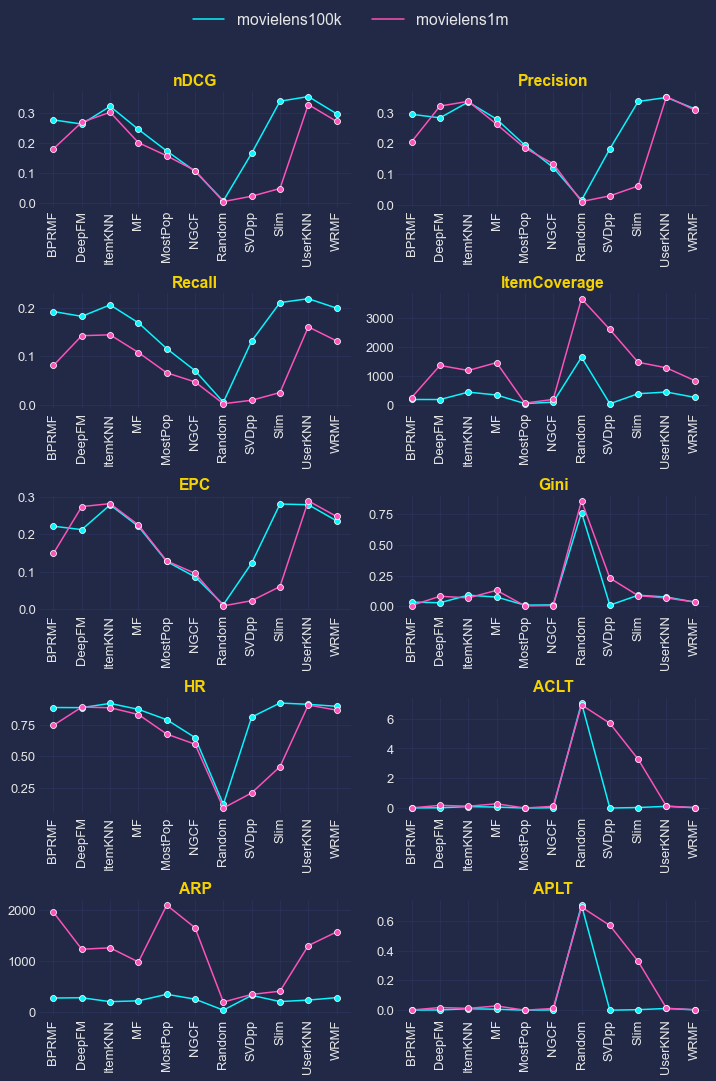
\includegraphics[width=\linewidth]{best1.png}
	\vspace*{-10mm}
	\caption{Σύνολα δεδομένων του Movielens, cut-off=10}
	\label{fig:best1}
\end{figure}
\begin{figure}[H]
	%\vspace{2px}%
	\centering
	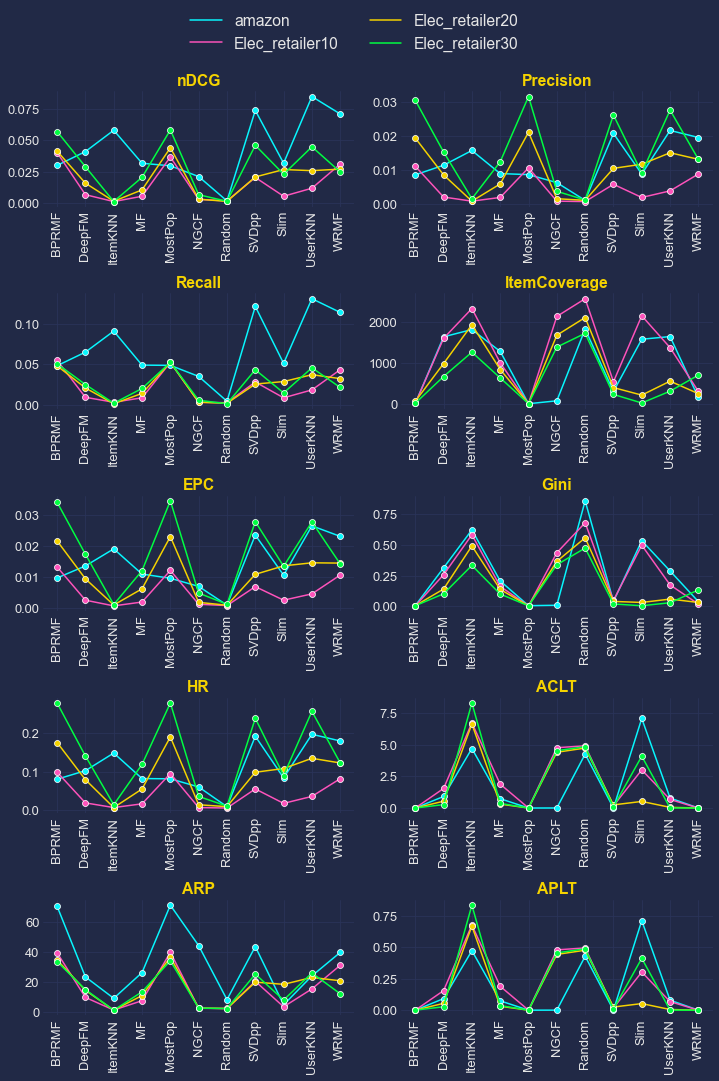
\includegraphics[width=\linewidth]{test8_updated.png}
		\vspace*{-10mm}
		\caption{Σύνολα δεδομένων του Elec\_retailer και του Amazon, cut-off=10}
%	\caption{Παράδειγμα προβολής καλύτερων αποτελεσμάτων και ανάλυσης cutoff.}
	\label{fig:best2}
\end{figure}

\begin{figure}[H]
	%\vspace{2px}%
	\centering
	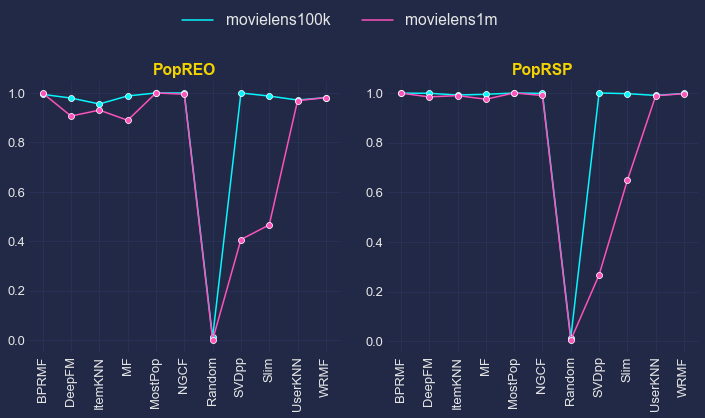
\includegraphics[width=\linewidth]{pop_movielens.png}
	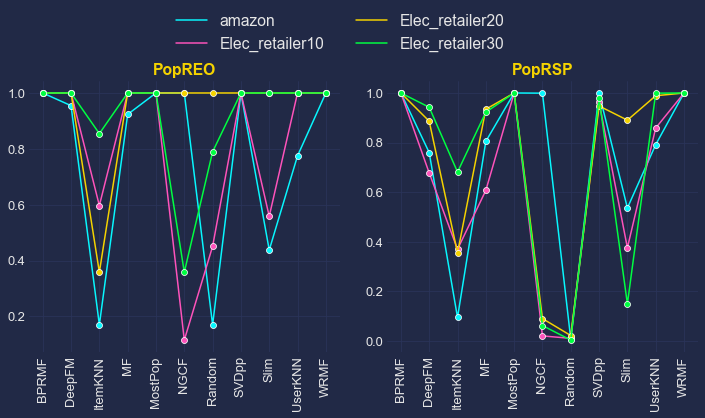
\includegraphics[width=\linewidth]{pop_ecommerce.png}
	\vspace*{-10mm}
	\caption{Μετρικές PopREO και PopRSP.}
	\label{fig:pop_metrics}
\end{figure}
\noindent\textbf{Popularity bias, diversity, novelty}\\
\noindent Ας εξετάσουμε πρώτα τι συμβαίνει με το novelty στα 4 σύνολα δεδομένων. Η μετρική EPC είναι εξ'ορισμού άρρηκτα συνδεδεμένη με την ακρίβεια και αυτό αποτελεί και την εξήγηση για το μηδενικό novelty του Random σε όλα τα σύνολα δεδομένων. Τα αντικείμενα που προτείνονται δεν πρέπει μόνο να μην τα έχει δει προηγουμένως ο χρήστης αλλά και να είναι σχετικά με τα ενδιαφέροντά του, κάτι που όπως είδαμε πριν στον Random δεν συμβαίνει. Το novelty στα σύνολα δεδομένων του Elec\_retailer και στο Amazon είναι σχεδόν μηδενικό, ενώ στα σύνολα δεδομένων του Movielens έχουμε πολύ καλύτερα αποτελέσματα, λογικά σε αυτό βοηθάει και το πολύ μεγάλο rating space. Αυτό αποτελεί μια ένδειξη πως η αραιότητα του μητρώου χρηστών-αντικειμένων δεν είναι το μόνο που επηρεάζει το novelty, αλλά και τα χαρακτηριστικά των δεδομένων.
Στο novelty ξεχωρίζει η πολύ κακή απόδοση των αλγορίθμων NGCF, BPRMF και SVD++. Στους υπόλοιπους αλγόριθμους έχουμε από μέτριες έως ικανοποιητικές τιμές, με τους δύο neighborhood based και τον DeepFM να ξεχωρίζουν, κάτι το οποίο δεν ισχύει στα σύνολα δεδομένων του Elec\_retailer. Κατά τη δημιουργία προτάσεων προς τους χρήστες, ένας από τους στόχους είναι να μην τους προτείνουμε αντικείμενα με τα οποία έχουν ήδη αλληλεπιδράσει, αλλά να τους οδηγήσουμε σε νέα μονοπάτια με αντικείμενα που ίσως τους ενδιαφέρουν. Χαρακτηριστικό παράδειγμα εδώ αποτελούν τα συστήματα συστάσεων μιας επιχείρησης ηλεκτρονικού εμπορίου, τα οποία έχουν την τάση να προτείνουν προϊόντα που ανήκουν στην ίδια ακριβώς κατηγορία με εκείνα που κάποιος πελάτης μόλις έχει αγοράσει. Μάλιστα συνεχίζουν να προβάλλουν τις ίδιες προτάσεις για ένα μεγάλο χρονικό διάστημα, προκαλώντας εκνευρισμό στον πελάτη και στερώντας του την ευκαιρία της ανακάλυψης προϊόντων ή και ολόκληρων κατηγοριών προϊόντων, που μπορεί και να αγνοούσε την ύπαρξή τους.

\noindent Στη συνέχεια, θα εξετάσουμε εάν κάποια αντικείμενα προτείνονται πιο συχνά σε σχέση με κάποια άλλα, και αν ναι σε τι βαθμό συμβαίνει αυτό. Αν εξαιρέσουμε τους αλγορίθμους itemKNN, NGCF και τον DeepFM που έχει σχετικά μέτρια επίδοση, στους υπόλοιπους αλγορίθμους παρατηρείται χαμηλό diversity στα σύνολα δεδομένων του Elec\_retailer και του Amazon, δηλαδή σε αυτά με πολύ υψηλή αραιότητα. \\
Εκ πρώτης όψεως από την μετρική APLT, θα έλεγε κάποιος πως όσο πιο αραιό είναι ένα μητρώο, τόσο λιγότερο είναι το popularity bias που εισάγεται. Αληθεύει όμως αυτό;
Ένα πρόβλημα με την μετρική APLT είναι πως μπορεί να έχει υψηλή τιμή ακόμη και εάν όλοι οι χρήστες έχουν λάβει το ίδιο σύνολο long-tail αντικειμένων. 
Σε όλους τους αλγορίθμους εκτός από τον NGCF και τον ItemΚΝΝ η μετρική PopReo είναι σχεδόν μηδενική για το Elec\_retailer.
Στο statistical parity τα πράγματα διαφοροποιούνται ελαφρώς κυρίως για τους αλγορίθμους MF και DeepFM, όσον αφορά τα σύνολα δεδομένων του Elec\_retailer, με τον αριθμό των χρηστών (και των αντικειμένων) να φαίνεται πως παίζει πολύ μεγαλύτερο ρόλο εδώ.
Άρα όταν λαμβάνουμε υπόψη και τις προτιμήσεις των χρηστών, η μεροληψία υπέρ των πιο δημοφιλών αντικειμένων είναι αρκετά πιο εμφανής.
Ο μόνος αλγόριθμος που φαίνεται να επηρεάζεται από το από την αραιότητα είναι ο SVD++.
Ας δούμε λίγο πιο προσεκτικά τι συμβαίνει με το popularity bias στο Elec\_retailer, με τη βοήθεια της μετρικής ARP.
Παρόλο που σχεδόν το 90\% των προϊόντων έχει λάβει 1-2 αξιολογήσεις, παρατηρούμε πως ο μέσος αριθμός των αξιολογήσεων των προϊόντων στις λίστες συστάσεων που έχουν παράξει οι αλγόριθμοι για κάθε χρήστη, είναι αρκετά μεγαλύτερος από όσο θα περιμέναμε και θα θέλαμε. Αυτό ισχύει για όλους τους αλγόριθμους εκτός από τον ItemKNN και τον NGCF, ενώ οι MF και DeepFM έχουν μέτρια επίδοση. Πρέπει να διευκρινιστεί πως ο μέσος αριθμός αξιολογήσεων αναφέρεται στις αξιολογήσεις στο σύνολο εκπαίδευσης και αποτελεί σοβαρή ένδειξη για την ύπαρξη του popularity bias.\\
Παρόμοια συμπεράσματα προκύπτουν και στο Amazon, με τις διαφορές να εντοπίζονται στους αλγορίθμους NGCF, itemKNN και WRMF. Αναλυτικότερα, στον itemKNN η ακρίβεια είναι αρκετά υψηλή στο Amazon και πάρα πολύ χαμηλή στο Elec\_retailer. Στον NGCF η διαφορά είναι ότι στον Amazon εισάγει αρκετή μεροληψία, ενώ στο Elec\_retailer ελάχιστη έως καθόλου.


\noindent Κατά την ανάλυση του αλγορίθμου BPRMF είδαμε ότι το φαινόμενο του popularity bias είναι αρκετά έντονο σε αυτόν, τα αντικείμενα που καλύπτονται είναι ελάχιστα, ενώ το diversity είναι εξίσου χαμηλό και εξηγήσαμε τους λόγους για τους οποίους συμβαίνει αυτό. Στα παραπάνω διαγράμματα μάλιστα παρατηρούμε πως όχι απλά είναι έντονο το φαινόμενο, αλλά έχει την χειρότερη επίδοση από όλους τους αλγορίθμους, σχεδόν ίδια με αυτή του αλγορίθμου MostPop σε όλα τα σύνολα δεδομένων. Εκτός όμως από τον BPRMF και οι περισσότεροι από τους υπόλοιπους αλγορίθμους φαίνεται πως έχουν την τάση να προτείνουν περισσότερο τα πιο δημοφιλή αντικείμενα, χωρίς να έχουν σχεδιαστεί για αυτόν τον σκοπό. Ακόμη, οι μετρικές μας δείχνουν πως οι neighborhood based αλγόριθμοι έχουν την τάση να μην προτείνουν συχνά αντικείμενα που ανήκουν στο long tail. Σε αυτό το σημείο θα πρέπει να υπενθυμίσουμε πως στον itemKNN για να δημιουργηθούν τα προτεινόμενα αντικείμενα προς τους χρήστες υπολογίζονται οι ομοιότητες των αντικειμένων με βάση τις αξιολογήσεις που έχουν λάβει από τους χρήστες, όπως φαίνεται και στον κάτωθι ψευδοκώδικα \cite{lindenAmazonComRecommendations2003}:
\begin{figure}[H]
	%\vspace{2px}%
	\centering
	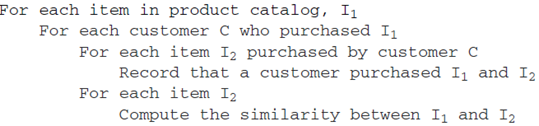
\includegraphics[]{itemknn_pseudocode.png}
	\caption{Ψευδοκώδικας αλγορίθμου itemKNN}
	\label{fig:item_pseudo}
\end{figure}
\noindent Όπως γίνεται εύκολα αντιληπτό, τα αντικείμενα που βρίσκονται στο long tail, έχουν λιγότερες πιθανότητες να επιλεχθούν εδώ. Αυτό επιβεβαιώνεται πλήρως και από τις μετρικές, ειδικά όσο αυξάνεται ο αριθμός των γειτόνων
Συνεπώς χρειάζεται λίγο πιο ενδελεχής έρευνα.
Εξετάζουμε τόσο το statistical parity (PopRSP) όσο και το equal opportunity (PopReo), που μας δείχνουν αν έχουν τις ίδιες πιθανότητες να προταθούν τα αντικείμενα που ανήκουν στο long-tail και τα αντικείμενα που ανήκουν στο head ή αν υπάρχει μεροληψία υπέρ των πιο δημοφιλών αντικειμένων (όσο μεγαλύτερη η τιμή τους, τόσο μεγαλύτερη η μεροληψία που υπάρχει). Ιδιαίτερη έμφαση δόθηκε στην PopREO, καθώς λαμβάνει υπόψη της και τις προτιμήσεις των χρηστών.

\noindent Η ύπαρξη του popularity bias σε ένα σύστημα προτάσεων ταινιών όπως το Movielens και σε οποιοδήποτε σύστημα ψυχαγωγίας υπάρχει στο διαδίκτυο αρχικά έχει άμεση επίπτωση στους καλλιτέχνες και στους δημιουργούς ενός προϊόντος. Εάν οι αλγόριθμοι συνηθίζουν να μεροληπτούν υπέρ των πιο δημοφιλών ταινιών στην προκειμένη περίπτωση, τότε οι νέοι καλλιτέχνες και οι ταινίες που δεν έχουν γίνει γνωστές στο ευρύ κοινό, θα μείνουν καταδικασμένοι για πάντα στην αφάνεια, ανεξαρτήτως της ποιότητάς τους. Αυτό ισχύει και στον χώρο του ηλεκτρονικού εμπορίου με τα λιγότερο δημοφιλή προϊόντα. Αρχικά, ζημιώνεται άμεσα η επιχείρηση που τα πουλάει, καθώς ένα πολύ μεγάλο ποσοστό των προϊόντων που μπορεί να αγγίζει και το 80\%, δηλαδή τα αντικείμενα που ανήκουν στο long-tail έχουν ελάχιστες πιθανότητες προβολής από τους χρήστες και συνεπώς αγοράς τους από αυτούς. Επίσης ζημιώνεται έμμεσα ο κατασκευαστής των προϊόντων που ανήκουν στο long-tail, διότι θα πουληθούν ελάχιστα κομμάτια και ενδεχομένως το κατάστημα να μην ξαναγοράσει τα συγκεκριμένα προϊόντα.\\


\newpage
\section{Μετριασμός μεροληψίας}
\noindent Για τον μετριασμό της μεροληψίας χρησιμοποιήθηκε ένας αλγόριθμος που ανήκει στην in-processing κατηγορία τεχνικών μετριασμού της μεροληψίας και τρεις αλγόριθμοι που ανήκουν στην post-processing κατηγορία. Ο in-processing αλγόριθμος που χρησιμοποιήθηκε είναι ο pairwise\_reg, ενώ οι post-processing είναι οι FAR, PFAR και Calibrated recommendations (στο εξής θα αναφέρεται ως ``cali") οι οποίες περιγράφονται αναλυτικά στην υποενότητα \ref{popularity bias}. Συμπληρωματικά, σε όλους τους πίνακες ως base αναφέρεται ο αρχικός αλγόριθμος, στα αποτελέσματα του οποίου εφαρμόσαμε τις τεχνικές μετριασμού τις μεροληψίας. Στο σημείο αυτό, θα αποτελούσε παράλειψη εάν δεν αναφέραμε πως κατά τη διάρκεια των πειραμάτων δοκιμάσαμε και έναν επιπλέον αλγόριθμο τον FA*IR. Ωστόσο ο χρόνος υπολογισμού των νέων λιστών συστάσεων σε όλα τα σύνολα δεδομένων, ήταν απαγορευτικά πολύ μεγάλος, καθώς ανάλογα με το σύνολο δεδομένων μπορεί να άγγιζε ή και να ξεπερνούσε την μία ώρα, ενώ και τα αποτελέσματα ήταν παρόμοια ή ακόμη και χειρότερα με τους υπόλοιπους αλγορίθμους που δοκιμάσαμε. Παρ'όλα αυτά, ο FA*IR είναι διαθέσιμος στην εφαρμογή μας, με την σύσταση να χρησιμοποιείται σε μικρά σύνολα δεδομένων, παρέχοντας σαφή προειδοποίηση προς τους χρήστες για το ζήτημα που υπάρχει.\\ H in-processing τεχνική επιλέχθηκε καθώς από την ανάλυση των αποτελεσμάτων φαίνεται πως το πρόβλημα στον BPRMF είναι αρκετά μεγάλο με τιμές που πλησιάζουν αυτές του MostPop, συνεπώς το πρόβλημα είναι στη δομή του αλγορίθμου και οι post-processing τεχνικές δεν θα βοηθήσουν. Στους post-processing αλγόριθμους δόθηκαν ως είσοδος οι λίστες συστάσεων που λάβαμε στο τρίτο βήμα του πειράματος από τους base αλγορίθμους συστάσεων, μεγέθους 100 για κάθε χρήστη. Οι αλγόριθμοι αυτοί λαμβάνουν επιπλέον ως είσοδο και μια λίστα όλων των αντικειμένων που υπάρχουν στο σύνολο δεδομένων, στην οποία έχουν επισημανθεί ποια από αυτά ανήκουν στο long tail και ποια ανήκουν στο head. Συνεπώς, δημιουργήθηκε για κάθε σύνολο δεδομένων ένα αρχείο το οποίο περιείχε τρεις στήλες:
\begin{enumerate}
	\item  \textbf{``itemid":} περιέχει τα IDs όλων των αντικειμένων που υπάρχουν
	\item \textbf{``feature":} η στήλη αυτή για 20\% των αντικειμένων που ανήκουν στο head, περιέχει την λέξη "head" και για τα υπόλοιπα αντικείμενα την λέξη ``long" 
	\item \textbf{``value":} περιέχει την τιμή 0 αν το αντικείμενο ανήκει σε προστατευόμενη ομάδα και την τιμή 1 διαφορετικά.
\end{enumerate}
  Για τον μετριασμό της μεροληψίας, επιλέχθηκαν οι λίστες συστάσεων από τους αλγορίθμους συστάσεων που διαπιστώθηκε στο προηγούμενο βήμα πως έλαβαν τις χαμηλότερες τιμές στις μετρικές που σχετίζονται με το popularity bias και το diversity. Στη συνέχεια ρυθμίστηκαν οι υπερπαράμετροι των αλγορίθμων μετριασμού μεροληψίας, δηλαδή ο αριθμός των αντικειμένων που θα περιέχει κάθε λίστα χρηστών στην οποία έχει γίνει ανακατάταξη και η παράμετρος κανονικοποίησης λ. Οι αλγόριθμοι εκτελέστηκαν για διάφορες τιμές του λ, πιο συγκεκριμένα λ=\{0.1 , 0.2 ,  0.5 , 0.7\}. Θα πρέπει να σημειωθεί ωστόσο πως στους πίνακες που ακολουθούν το λ είναι ίσο με 0.5 καθώς η τιμή αυτή εξασφαλίζει τη βέλτιστη ισορροπία ανάμεσα στην ακρίβεια και στην μεροληψία, όπως διαπιστώθηκε από δοκιμές που πραγματοποιήσαμε μέσω της εφαρμογής. Εάν κάποιος δεν ενδιαφέρεται τόσο για την ακρίβεια, μπορεί να θέσει την τιμή του λ στο εύρος [0.6 , 0.7]. Αφού δόθηκαν ως είσοδος οι δύο προαναφερθείσες λίστες στους postprocessing αλγορίθμους, εκείνοι παρήγαγαν ως έξοδο τις νέες re-ranked λίστες συστάσεων μεγέθους 30 για κάθε χρήστη.  Επίσης, σε όλες τις μετρικές έχει γίνει στρογγυλοποίηση στα τρία δυαδικά ψηφία, εκτός από τις μετρικές Recall, EPC που έγινε στα τέσσερα, την μετρική ARP στα 2 και φυσικά την μετρική ItemCoverage που είναι ακέραιος αριθμός. 
Τέλος, διατηρήθηκαν τα ίδια σύνολα εκπαίδευσης και δοκιμής που χρησιμοποιήθηκαν και στο προηγούμενο βήμα. Στις παραγράφους που ακολουθούν περιγράφεται η επίδραση των αλγορίθμων μετριασμού μεροληψίας στα διάφορα σύνολα δεδομένων, δίνοντας ιδιαίτερη έμφαση στον Cali, καθώς όπως θα εξηγήσουμε πετυχαίνει (σχεδόν) πάντα την μεγαλύτερη μείωση της μεροληψίας. Αναφερόμαστε αρχικά αρκετά αναλυτικά στην επίδραση που έχει ο αλγόριθμος στα δύο σύνολα δεδομένων του Movielens και στο τέλος αναφερόμαστε στην επίδραση που έχει στο σύνολο του Amazon. Αυτό έγινε διότι όπως θα εξηγήσουμε σε επόμενη παράγραφο, στο σύνολο δεδομένων έχουμε πάρα πολύ χαμηλή ακρίβεια και ενδεχομένως τα συμπεράσματα που θα προκύψουν να μην ασφαλή.\\

\begin{table}[H]
\centering	
\caption {Μετριασμός μεροληψίας στον αλγόριθμο WRMF} \label{tab:WRMF_best1} 
\footnotesize
\centerline{
\begin{tabular}{l rrrr|rrrr|rrrr}
	\toprule
	& \multicolumn{4}{c}{Movielens100k}	& \multicolumn{4}{c}{Movielens1M} & \multicolumn{4}{c}{Amazon}\\ \cmidrule(lr){2-5}
  \cmidrule(lr){6-9}
 \cmidrule(lr){10-13}
	{} & {\textbf{base}} & {\textbf{FAR}} & {\textbf{PFAR}} & \textbf{cali} & {\textbf{base}} & {\textbf{FAR}} & {\textbf{PFAR}} & \textbf{cali} & {\textbf{base}} & {\textbf{FAR}} & {\textbf{PFAR}} & \textbf{cali} \\
	 \midrule 
nDCG &	\textbf{0.339} &  0.333 & 0.336 & 0.322 & \textbf{0.298} & 0.286 & 0.286 & 0.282  &\textbf{0.094} & 0.089 & 0.091 & 0.073 \\
Prec. &	0.207 & \textbf{ 0.208} & 0.207 & \textbf{0.208} &\textbf{ 0.220} & 0.219 & 0.219 & 0.219& \textbf{0.012} & 0.011 & 0.011 & 0.010 \\
Recall	& 0.3616 & 	0.3617 & 0.3625 & \textbf{0.3631}& \textbf{0.2576} & 0.2560 & 0.2560 & 0.2572 & \textbf{0.1996} & 0.1887 & 0.1935 & 0.1779\\
ΙC &	505 & 	571 & 560 & \textbf{607} & 1445 & 1517 & 1517 & \textbf{1594} & 349 & 654 & 631 & \textbf{704}\\
EPC	& 0.1790 &	0.1789 & \textbf{0.1792} & 0.1775 & \textbf{0.1960} & 0.1930 & 0.1933 & 0.192 &\textbf{0.0150} & 0.0146 & 0.0149 & 0.0119\\
Gini	& 0.071 &	0.078 & 0.077 &\textbf{ 0.080} & 0.064 & 0.072 & 0.072 & \textbf{0.075} &0.076 & 0.109 & 0.102 &\textbf{ 0.123}\\
HR	&\textbf{ 0.976} &\textbf{ 0.976} &\textbf{ 0.976 }& 0.975 & 0.956 & \textbf{0.957} & \textbf{0.957} & \textbf{0.957} &\textbf{ 0.300} & 0.286 & 0.292 & 0.273\\
ACLT	& 0.164 &	0.348 & 0.298 & \textbf{0.407} & 0.381 & 0.413 & 0.414  & \textbf{0.558} & 0.034 & 0.543 & 0.387 & \textbf{0.986}\\
ARP	& 237.52 &	 231.19 & 232.61 & \textbf{230.41} & 1331.21 & 1302.38 &1302.49 & \textbf{1297.07} &31.89 & 28.02 & 29.02& \textbf{26.08} \\
APLT	& 0.005 &	0.012 & 0.010 & \textbf{0.014} & 0.013 & 0.014 & 0.014  & \textbf{0.019} & 0.001 & 0.018 & 0.013 & \textbf{0.033} \\
PREO	& 0.969 &	0.952 &  0.956 &\textbf{ 0.942} &0.944 & 0.937 & 0.936 & \textbf{0.904} &0.991 & 0.964 & 0.959 & \textbf{0.930}\\
PRSP	& 0.995 &  0.990 & 0.991 & \textbf{0.989} & 0.989 & 0.988 & 0.988 & \textbf{0.984} & 0.997 & 0.951 & 0.965 & \textbf{0.912}\\
	\bottomrule 
\end{tabular}
}
\end{table}
\noindent Ο πρώτος αλγόριθμος στον οποίο δοκιμάσαμε να μετριάσουμε την μεροληψίας είναι ο WRMF. Με τον αλγόριθμο cali έχουμε αύξηση 20\% στο Movielens100k και 10\% στο Movielens1M στην κάλυψη των αντικειμένων. Στις μετρικές popularity bias, παρατηρείται μια μείωση της τάξης του 3\% και 2.5\% στο ARP, στο ACLT έχουμε πάρα πολύ μεγάλη αύξηση 148\% και 46.5\% και στο popREO μία αρκετά μικρή βελτίωση 3\% 4\%, στα ml100k και ml1m αντίστοιχα. στο Gini 11\% και 17\% ml100k και ml1m αντίστοιχα. Στις μετρικές ακρίβειας, το precision, το HR και το recall μένουν σχεδόν αμετάβλητα, ενώ στο nDCG έχουμε μια μείωση της τάξης του 5\% και στα 2 σύνολα δεδομένων. Επομένως με μια σχετικά μικρή μείωση μόνο στο nDCG, βελτιώνουμε όλες τις υπόλοιπες μετρικές. \\\\
Ακολουθεί η ανάλυση για τον αλγόριθμο SLIM, για όλες τις μετρικές το πρώτο ποσοστό που αναφέρεται αντιστοιχεί στο ml100k και το δεύτερο στο ml1m. Στον αλγόριθμο Slim παρατηρούμε μια αρκετά μεγαλύτερη μείωση 17\% και 11.5\% στην τιμή του nDCG. Μικρότερη αλλά όχι αμελητέα είναι η μείωση στο precision (6.5\% και 6\%), ενώ ακόμα πιο μικρή είναι στο Recall (4\% και στα δύο σύνολα δεδομένων). Παράλληλα, o συγκεκριμένος αλγόριθμος μετριασμού της μεροληψίας παράγει κατά 17\% και κατά 12\% περισσότερα αντικείμενα, στα ml100k και ml1m αντίστοιχα. Τα ποσοστά αυτά είναι ελαφρώς μεγαλύτερα από τον WRMF, όπου ο base αλγόριθμος κάλυπτε λιγότερα αντικείμενα από τον Slim. Σε ό,τι έχει να κάνει με το popularity bias  η βελτίωση που έχουμε αντικατοπτρίζεται με την μείωση  10\% και 9.4\% στη μετρική ARP, με την τεράστια αύξηση, 195\% και 86\% στην APLT, και την μείωση 13\% και 8\% στην popREO. Ωστόσο, στην popRSP όπου το πρόβλημα είναι πολύ μεγαλύτερο, η βελτίωση είναι αρκετά μικρότερη (-3.6\% και -2\%). Τέλος, μικρή αύξηση της τάξης του 26.6\% και 17.2\% έχουμε στη μετρική Gini.\\
\begin{table}[H]
	\centering	
	\caption {Μετριασμός μεροληψίας στον αλγόριθμο Slim} \label{tab:Slim_best1} 
	\footnotesize
	\centerline{
\begin{tabular}{l rrrr|rrrr|rrrr}
	\toprule
	& \multicolumn{4}{c}{Movielens100k}	& \multicolumn{4}{c}{Movielens1M} & \multicolumn{4}{c}{Amazon}\\ \cmidrule(lr){2-5}
	\cmidrule(lr){6-9}
	\cmidrule(lr){10-13}
	{} & {\textbf{base}} & {\textbf{FAR}} & {\textbf{PFAR}} & \textbf{cali}& {\textbf{base}} & {\textbf{FAR}} & {\textbf{PFAR}} &  \textbf{cali} &\textbf{base} & {\textbf{FAR}} & {\textbf{PFAR}} & \textbf{cali}\\
		\midrule 
		nDCG &	\textbf{0.386} &  0.370 & 0.384 & 0.319 &\textbf{ 0.261} & 0.247 & 0.253 & 0.231 & 0.049 & \textbf{0.064} & 0.063 & 0.059 \\
		Prec. &	\textbf{0.2277} &  0.2197 & 0.2265 & 0.2130 & \textbf{0.2040} & 0.1940 & 0.1970 & 0.1912 & 0.0065 & \textbf{0.0080} & 0.0079 & \textbf{0.0080} \\
		Recall	& \textbf{0.3949} & 	0.3810 & 0.3929 & 0.3780 &\textbf{ 0.2404} & 0.2283 & 0.2314 & 0.2302 & 0.1179 & 0.1377 & 0.1370 & 0.1373 \\
		ΙC &	609 & 	690 & 653 & \textbf{711} & 1396 & 1504 & 1484 &\textbf{ 1563} & 1780 & \textbf{1784} & \textbf{1784} & \textbf{1784} \\
		EPC	&\textbf{ 0.2111} &	0.2045 & 0.2108 & 0.1877 & \textbf{0.1952} & 0.1864 & 0.1900 & 0.1772 & 0.0080 & \textbf{0.0107} & 0.0105 & 0.0099 \\
		Gini	& 0.150 &	0.181 & 0.163 & \textbf{0.190} & 0.1449 & 0.1667 & 0.1622 & \textbf{0.1697} &\textbf{ 0.7106} & 0.5506 & 0.5694 & 0.5490\\
		HR	& \textbf{0.986} & 0.979 & 0.983 & 0.981 &\textbf{ 0.949} & 0.943 & 0.944 & 0.944 &0.182 &\textbf{ 0.215} & 0.213 & \textbf{0.215} \\
		ACLT	& 0.602 &	1.460 & 0.920 & \textbf{1.771} & 0.649 & 1.046 & 0.940 & \textbf{1.221} &\textbf{ 14.777 }& 10.876 & 11.229 & 10.804 \\
		ARP	& 176.98 &	 162.89 & 171.54 & \textbf{158.59} & 817.31 & 750.68 & 766.75 & \textbf{740.25} & \textbf{6.98} & 10.43 & 10.13 & 10.46 \\
		APLT	& 0.020 &	0.049 & 0.031 & \textbf{0.059} & 0.022 & 0.035 & 0.031 &\textbf{0.041} &\textbf{ 0.493} & 0.363 & 0.374 & 0.360 \\
		PREO	& 0.930 &	0.864 &  0.908 &\textbf{ 0.806} & 0.908 &  0.882 & 0.890 & \textbf{0.841} & \textbf{0.056} & 0.178&0.157 & 0.180\\
		PRSP	& 0.983 &  0.957 & 0.973 & \textbf{0.948} & 0.981& 0.969 & 0.972 & \textbf{0.964} & 0.136 & 0.130&\textbf{0.105}&0.135\\
		\bottomrule 
	\end{tabular}
}
\end{table}
\noindent Μια ενδιαφέρουσα παρατήρηση εδώ είναι πως εάν επιχειρήσουμε σε ένα σύνολο δεδομένων με πολύ μεγάλη αραιότητα, όπου ο base αλγόριθμος μας έχει δώσει πολύ χαμηλή ακρίβεια και ελάχιστη μεροληψία, τότε όλοι οι αλγόριθμοι re-ranking έχουν αρκετά διαφορετική επίδραση από τα σύνολα δεδομένων του Movielens και από ότι ενδεχομένως θα αναμέναμε. Πιο συγκεκριμένα, βελτιώνουν την ακρίβεια και εισάγουν λίγη περισσότερη μεροληψία, αυξάνοντας κατά πολύ λίγο και τα αντικείμενα που καλύπτονται. Μια υπόθεση που μπορούμε να κάνουμε εδώ είναι πως οι re-ranking αλγόριθμοι προσπαθούν να βρουν το καλύτερο δυνατό αντιστάθμισμα ανάμεσα στην ακρίβεια και στην μεροληψία και για να γίνει αυτό εδώ θα πρέπει να «θυσιαστεί» η μεροληψία και όχι η ακρίβεια, καθότι εκεί έχουμε πάρα πολύ καλή επίδοση και δεν επηρεάζει πολύ τα αποτελέσματα μια ελαφρά εισαγωγή επιπλέον μεροληψίας. Ωστόσο ένα σημαντικό θέμα που φαίνεται να προκύπτει εδώ, είναι η σημαντική πτώση που παρατηρείται στην τιμή του diversity. Αυτή είναι η μία περίπτωση στο Amazon για τον αλγόριθμο Slim. Η άλλη περίπτωση, είναι να λειτουργήσει κλασικά δηλαδή να μειώσει την μεροληψία, μειώνοντας όμως ταυτόχρονα και την ακρίβεια, όπως συμβαίνει στον αλγόριθμο DeepFM και στον MF που έχει λίγο καλύτερη ακρίβεια από τον Slim.
\noindent Στον αλγόριθμο DeepFM έχουμε μια αύξηση στο nDCG της τάξης του 10\%, 13\% και 20\% στα σύνολα δεδομένων με την σειρά που εμφανίζονται στον πίνακα. Στην κάλυψη των αντικειμένων, τα αντικείμενα που προτείνονται αυξάνονται κατά 24\% στο ML1M και 8.4\% στο ml100k, ενώ στο Amazon έχουμε την κάλυψη 10 επιπλέον αντικειμένων. Επιπρόσθετα, στην μετρική Gini την μεγαλύτερη αύξηση την παρατηρούμε στο ML1M (30\%), ενώ στα υπόλοιπα δύο τα νούμερα είναι αρκετά μικρότερη, 11\% και 12\% αντίστοιχα. Η μείωση στο ARP είναι αρκετά μικρότερη από το Slim (4\%, 9\%). Στο σύνολο Amazon δεν αυξάνει την μεροληψία όπως στον Slim, αλλά την μειώνει επιτυγχάνοντας παρόμοια νούμερα με εκείνα που είδαμε στο WRMF ως προς το ποσοστό μείωσης.
Τέλος, στον αλγόριθμο MF προκύπτουν παρόμοια συμπεράσματα αν μελετήσουμε προσεκτικά τον πίνακα \ref{tab:MF_best1}.
\begin{table}[H]
	\centering	
	\caption {Μετριασμός μεροληψίας στον αλγόριθμο DeepFM} \label{tab:DeepFM_best1} 
	\footnotesize
	\centerline{
	\begin{tabular}{l rrrr|rrrr|rrrr}
		\toprule
		& \multicolumn{4}{c}{Movielens100k}	& \multicolumn{4}{c}{Movielens1M} & \multicolumn{4}{c}{Amazon}\\ \cmidrule(lr){2-5}
		\cmidrule(lr){6-9}
		\cmidrule(lr){10-13}
		{} & {\textbf{base}} & {\textbf{FAR}} & {\textbf{PFAR}} & \textbf{cali} & {\textbf{base}} & {\textbf{FAR}} & {\textbf{PFAR}} & \textbf{cali} & {\textbf{base}} & {\textbf{FAR}} & {\textbf{PFAR}} & \textbf{cali} \\
		\midrule 
		nDCG & \textbf{0.318}	& 0.306 & 0.308 & 0.285 & \textbf{0.294} & 0.275 & 0.278 & 0.256 & \textbf{0.055} & 0.051 & 0.053 & 0.044  \\
		Prec. &\textbf{ 0.2048} & 0.1988 & 0.2005 & 0.1983 & \textbf{0.2330} & 0.2221 & 0.2239 & 0.2208 & \textbf{ 0.0068} & 0.0065 & 0.0066 & 0.0064\\
		Recall	&\textbf{ 0.3651} & 0.3549 & 0.3573 & 0.3529 &\textbf{0.2850} & 0.2741 & 0.2764 &0.2747 & \textbf{0.1174} & 0.1120 & 0.1138 & 0.1110\\
		ΙC & 356	& 380 & 373 & \textbf{443} & 2124 & 2165 & 2152 & \textbf{2303} & 1812 & 1818 & 1817 & \textbf{1822} \\
		EPC	& \textbf{0.172}3 & 0.1666 & 0.1680 & 0.1624 &\textbf{0.2168} & 0.2045 & 0.2064 & 0.1971 & \textbf{0.0091}& 0.0084 & 0.0087& 0.0073\\
		Gini	& 0.071 & 0.073 & 0.072 &  \textbf{0.079} &0.144 & 0.176 & 0.170 & \textbf{0.187} & 0.451 & 0.486 & 0.476 & \textbf{0.504}\\
		HR	& 0.979 & 0.982 &\textbf{ 0.983} &0.979 & \textbf{0.975} & 0.974 & 0.973 & 0.972 & \textbf{0.184} & 0.174 & 0.178 & 0.173\\
		ACLT	& 0.093 & 0.128 & 0.119 &\textbf{0.386} & 1.31 & 1.93 & 1.77 & \textbf{2.37} & 4.42 & 4.86 & 4.72 & \textbf{5.18}\\
		ARP	& 227.34 & 223.48 & 224.57 & \textbf{216.54} & 1016.21 & 942.10 & 957.98 & \textbf{924.42} & 18.30 & 17.34 & 17.62 &\textbf{ 16.91}\\
		APLT	& 0.0031& 0.0043 & 0.0040 & \textbf{0.0129} & 0.044 & 0.064 & 0.059 & \textbf{0.079} & 0.147 & 0.162 & 0.157 & \textbf{0.173}\\
		PREO	& 0.970 & 0.964 & 0.965 & \textbf{0.920} &0.794 & 0.763 & 0.770 & \textbf{0.687} & 0.793 & 0.757 & \textbf{0.755} & 0.760 \\
		PRSP	& 0.997 & 0.996 & 0.997 & \textbf{0.989} & 0.961 & 0.942 & 0.947 & \textbf{0.928} & 0.621 & 0.585 & 0.597 & \textbf{0.560}\\
		\bottomrule 
	\end{tabular}
}
\end{table}
\begin{table}[H]
	\centering	
	\caption {Μετριασμός μεροληψίας στον αλγόριθμο MF} \label{tab:MF_best1}
		\footnotesize
	\centerline{ 
	\begin{tabular}{l rrrr|rrrr|rrrr}
		\toprule
		& \multicolumn{4}{c}{Movielens100k}	& \multicolumn{4}{c}{Movielens1M} & \multicolumn{4}{c}{Amazon}\\ \cmidrule(lr){2-5}
		\cmidrule(lr){6-9}
		\cmidrule(lr){10-13}
		{} & {\textbf{base}} & {\textbf{FAR}} & {\textbf{PFAR}} & \textbf{cali} & {\textbf{base}} & {\textbf{FAR}} & {\textbf{PFAR}} & \textbf{cali} & {\textbf{base}} & {\textbf{FAR}} & {\textbf{PFAR}} & \textbf{cali}  \\
		\midrule 
		nDCG & \textbf{0.305} & 0.298 & 0.300 & 0.268 & \textbf{0.241} & 0.231 & 0.236 & 0.222 & \textbf{0.043} & 0.037 & 0.038 & 0.032\\
		Prec. & \textbf{0.2090} & 0.2046 & 0.2060 & 0.1947 &\textbf{0.2076} & 0.2000 & 0.2029 & 0.1968 & \textbf{0.0054} & 0.0051 & 0.0051 & 0.0051\\
		Recall	& \textbf{0.3610} & 0.3545 & 0.3567 & 0.3447 & \textbf{0.2425} & 0.2341 & 0.2375 & 0.2343 & \textbf{0.0906} & 0.0856 & 0.0858 & 0.0854 \\
		ΙC & 495	& 510 & 504 & \textbf{597} & 1818 & 1833 & 1825 & \textbf{1926} & 1656 & 1707 & 1703 &\textbf{1713}\\
		EPC	&\textbf{0.1797} & 0.1757 & 0.1769 & 0.1633 & \textbf{0.1872} & 0.1807 & 0.1837 & 0.1748 & \textbf{0.0073} & 0.0063 & 0.0065 & 0.0054\\
		Gini	& 0.118 & 0.121 & 0.121 & \textbf{0.143} & 0.154 & 0.175 & 0.169 & \textbf{0.185} & 0.346 & 0.398 & 0.392 & \textbf{0.404} \\
		HR	& 0.973 & 0.977 & \textbf{0.978} &0.966 & \textbf{0.953} & 0.951 & 0.951 & 0.950 & \textbf{0.147} & 0.141 & 0.141 &0.141\\
		ACLT	& 0.524 & 0.584 & 0.573 & \textbf{1.047 }& 1.16 & 1.45 & 1.34 & \textbf{1.74} & 4.12 & 5.06 & 4.95 & \textbf{5.28}\\
		ARP	& 194.47 & 191.15 & 192.06 & \textbf{177.87} & 940.00 & 883.24 & 901.49 & \textbf{862.31} & 19.42 & 17.63 & 17.85 &\textbf{17.41}\\
		APLT	& 0.017 & 0.019 & 0.019 & \textbf{0.035} & 0.039 & 0.048 & 0.045 & \textbf{0.058} &0.137&0.169 & 0.165 &\textbf{0.176}\\
		PopREO	& 0.951 & 0.949 & 0.951 &\textbf{0.888}& 0.866 & 0.846 & 0.855 &\textbf{ 0.795} & 0.809 & 0.793 & 0.813 &\textbf{ 0.791}\\
		PopRSP	& 0.985 & 0.983 & 0.984 & \textbf{0.970} & 0.965 & 0.957 & 0.960 &\textbf{0.948} & 0.645 & 0.570 & 0.578 &\textbf{ 0.552}\\
		\bottomrule 
	\end{tabular}
}
\end{table}
\noindent Δοκιμάσαμε να εφαρμόσουμε και τις τρεις τεχνικές και στο σύνολο του Amazon, παρόλο που εκεί το μεγάλο πρόβλημα είναι η πάρα πολύ χαμηλή ακρίβεια και όχι το popularity bias, προκειμένου να εξετάσουμε την επίδραση που θα έχουν και σε μια τέτοια περίπτωση. Το βασικό συμπέρασμα που προκύπτει ύστερα από την εφαρμογή τριών post-processing τεχνικών είναι πως για τους αλγορίθμους όπου δεν είναι αρκετά έντονο το πρόβλημα του popularity bias είναι αρκετά αποτελεσματικές και οι τρεις τεχνικές. Ωστόσο σε διαφορετική περίπτωση υπάρχει μεν βελτίωση αλλά όχι τόσο μεγάλη ώστε να θεωρούμε πως αποτελούν μια καλή λύση για τον μετριασμό της μεροληψίας. Στην περίπτωση αυτή θα πρέπει να αναζητηθούν διαφορετικού τύπου τεχνικές, με τις in-processing που επιδρούν στη δομή του αλγορίθμου προσπαθώντας να επιτύχουν ένα βέλτιστο αντιστάθμισμα ανάμεσα στην μεροληψία και στην ακρίβεια ή και ένα συνδυασμό είδους τεχνικών in-processing, post-processing και pre-processing να αποτελούν δύο πολύ καλές επιλογές. Από τους τρεις αλγορίθμους που δοκιμάσαμε για όλους τους αλγορίθμους και όλα τα σύνολα δεδομένων είχαμε το ίδιο μοτίβο συμπεριφοράς. Μεγαλύτερη μείωση της μεροληψίας παρατηρήθηκε στον Calibrated recommendations, με τον far να ακολουθεί και τον pfar να έχει την χειρότερη επίδοση. Αυτό φυσικά ισχύει και για την κάλυψη των αντικειμένων και στο diversity. Ενώ όπως ήταν αναμενόμενο το τελείως αντίθετο συμβαίνει στην ακρίβεια, αν και στις περισσότερες περιπτώσεις η μείωση στο Precision, στο Recall και στο HR είναι σχεδόν αμελητέα και είναι αρκετά πιο αισθητή στο nDCG.\\
Η in-processing τεχνική που δοκιμάσαμε στο σύνολο δεδομένων Movielens1M αποτελεί μέρος ενός ευρύτερου αλγορίθμου που συνδυάζει 3 τεχνικές μια pre-processing, μια in-processing (αυτή που δοκιμάσαμε) και μια post-processing. Η ακρίβεια από ότι παρατηρούμε μειώνεται πάρα πολύ ωστόσο εάν εφαρμόσουμε την in-processing τεχνική που προτείνεται, ενδεχομένως να βελτιώνεται αισθητά, χωρίς μάλιστα να επηρεάζει την μεροληψία που εισάγεται. Αυτό δεν εντάσσεται στα πλαίσια της παρούσας εργασίας και αφήνεται για μελλοντική εργασία. Εάν μάλιστα τον συγκρίνουμε με τον αλγόριθμο BPRMF που είναι και εκείνος pairwise και αποτελεί την βάση του αλγορίθμου που βελτίωσε αυτή η τεχνική, τότε είναι ξεκάθαρο πως ναι μεν το ζήτημα της μεροληψίας παραμένει σχετικά υψηλό, εντούτοις η βελτίωση είναι κατά πολύ μεγαλύτερη από όλες τις post-processing τεχνικές που δοκιμάσαμε σε οποιονδήποτε από τους αλγορίθμους. Η διαφορά μάλιστα γίνεται ακόμα πιο αισθητή σε μικρά cut-off κάτι ιδιαίτερα σημαντικό για μία πληθώρα συστημάτων που παρέχουν μικρό αριθμό συστάσεων προς τους χρήστες. 
\begin{figure}[H]
	%\vspace{2px}%
	\centering
	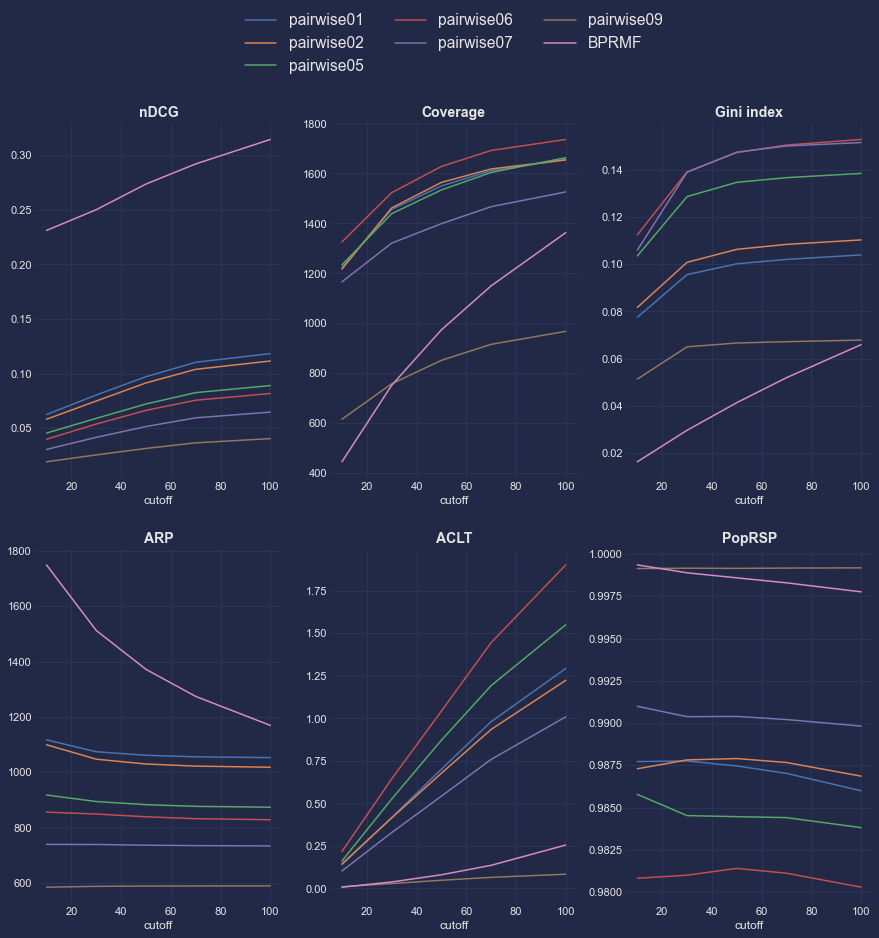
\includegraphics[width=\linewidth]{pairwise.png}
	\caption{Αλγόριθμος pairwise\_reg και σύγκριση με τον BPRMF}
	\label{fig:pair}
\end{figure}

